% !Mode:: "TeX:UTF-8"
% !TEX encoding = UTF-8 Unicode

%----------------------------------------------------------------------------------------
% 机器翻译:统计建模与深度学习方法
% Machine Translation: Statistical Modeling and Deep Learning Methods
%
% Copyright 2020
% 肖桐(xiaotong@mail.neu.edu.cn) 朱靖波 (zhujingbo@mail.neu.edu.cn)
%----------------------------------------------------------------------------------------

%----------------------------------------------------------------------------------------
%    CONFIGURATIONS configurations
%----------------------------------------------------------------------------------------
\renewcommand\figurename{图}%将figure改为图
\renewcommand\tablename{表}%将figure改为图
\chapterimage{fig-NEU-5.jpg} % Chapter heading image

%----------------------------------------------------------------------------------------
%	CHAPTER 4
%----------------------------------------------------------------------------------------

\chapter{基于短语和句法的机器翻译模型}

\parinterval 机器翻译的一个问题是要定义翻译的基本单元是什么。比如,可以像第三章介绍的那样,以单词为单位进行翻译,即把句子的翻译看作是单词之间对应关系的一种组合。基于单词的模型是符合人类对翻译问题的认知的,因为单词本身就是人类加工语言的一种基本单元。另一方面,在进行翻译时也可以使用一些更``复杂''的知识。比如,很多词语间的搭配需要根据语境的变化进行调整,而且对于句子结构的翻译往往需要更上层的知识,如句法知识。因此,在对单词翻译进行建模的基础上,需要探索其他类型的翻译知识,使得搭配和结构翻译等问题可以更好地被建模。

\parinterval 本章会介绍基于短语和基于句法的翻译模型。在过去二十年中,它们一直是机器翻译的主流方法。相比于基于单词的翻译模型,基于短语和基于句法的模型可以更好地对单词之间的依赖关系进行描述,同时可以对句子的上层结构进行有效的表示。这些方法也在相当长的一段时期内占据着机器翻译的统治地位。虽然近些年随着神经机器翻译的崛起,基于短语和基于句法的统计翻译模型有些``降温'',但是它仍然是机器翻译的主要框架之一,其中的思想和很多技术手段对今天的机器翻译研究仍然有很好的借鉴意义。

%----------------------------------------------------------------------------------------
%    NEW SECTION
%----------------------------------------------------------------------------------------

\section{翻译中的结构信息}

\parinterval 首先,回顾一下基于单词的统计翻译模型是如何完成翻译的。图\ref{fig:4-1}展示了一个实例。其中,左侧是一个单词的``翻译表'',它记录了源语言(中文)单词和目标语言(英文)单词之间的对应关系,以及这种对应的可能性大小(用P表示)。在翻译时,会使用这些单词一级的对应,生成目标语言译文。比如,图\ref{fig:4-1}右侧就展示了一个基于词的模型生成的翻译结果,其中$\mathbf{s}$和$\mathbf{t}$分别表示源语言和目标语言句子,单词之间的连线表示两个句子中单词一级的对应。

%----------------------------------------------
\begin{figure}[htp]
\centering
\begin{tabular}{l r}
\subfigure{%%%------------------------------------------------------------------------------------------------------------
%%% 基于单词的模型的问题


{\small
\begin{tabular}{l | l}
单词翻译表 & P \\ \hline
我 $\to$ I & 0.6 \\
喜欢 $\to$ like & 0.3 \\
绿 $\to$ green & 0.9 \\
茶 $\to$ tea & 0.8 \\
\end{tabular}
}

} & \subfigure{\begin{minipage}[c]{0.35\linewidth}
\begin{tikzpicture}

\begin{scope}
{\small
\node [anchor=west] (s1) at (0,0) {我};
\node [anchor=west] (s2) at ([xshift=1.0em]s1.east) {喜欢};
\node [anchor=west] (s3) at ([xshift=1.0em]s2.east) {{\color{ugreen} 绿}};
\node [anchor=west] (s4) at ([xshift=1.07em]s3.east) {茶};
\node [anchor=east] (s) at (s1.west) {$\textbf{s}=$};
}
\end{scope}

{
\begin{scope}[yshift=-2.0em]
{\small
\node [anchor=west] (t1) at (0.35em,0) {I};
\node [anchor=west] (t2) at ([xshift=0.8em,yshift=-0.0em]t1.east) {like};
\node [anchor=west] (t3) at ([xshift=1.0em,yshift=-0.2em]t2.east) {green};
\node [anchor=west] (t4) at ([xshift=0.78em,yshift=0.1em]t3.east) {tea};
\node [anchor=east] (t) at ([xshift=-0.3em]t1.west) {$\textbf{t}=$};
}
\end{scope}

\draw [-] (s1.south) -- (t1.north);
\draw [-] (s2.south) ..controls +(south:0.5em) and +(north:0.5em).. (t2.north);
\draw [-] (s3.south) ..controls +(south:0.5em) and +(north:0.5em).. (t3.north);
\draw [-] (s4.south) -- (t4.north);
}%visible<2->

\end{tikzpicture}
\end{minipage}} \\
\end{tabular}
\caption{基于单词的翻译实例}
\label{fig:4-1}
\end{figure}
%-------------------------------------------

\parinterval 图\ref{fig:4-1}体现的是一个典型的基于单词对应关系的翻译方法。它非常适合{\small\bfnew{组合性翻译}}\index{组合性翻译}(Compositional Translation)\index{Compositional Translation}的情况,也就是通常说的直译。不过,自然语言作为人类创造的高级智能的载体,远比想象的复杂。比如,即使是同一个单词,词义也会根据不同的语境产生变化。

%----------------------------------------------
\begin{figure}[htp]
\centering
\begin{tabular}{l r}
\subfigure{%%%------------------------------------------------------------------------------------------------------------
%%% 基于单词的模型的问题
{\small
\begin{tabular}{l | l}
单词翻译表 & P \\ \hline
我 $\to$ I & 0.6 \\
喜欢 $\to$ like & 0.3 \\
红 $\to$ red & 0.8 \\
红 $\to$ black & 0.1 \\
茶 $\to$ tea & 0.8\\
\end{tabular}
}

} & \subfigure{%%%------------------------------------------------------------------------------------------------------------
%%% 基于单词的模型的问题
\begin{minipage}[c]{0.35\linewidth}
\vspace{1em}
\begin{tikzpicture}

\begin{scope}
{\small
\node [anchor=west] (s1) at (0,0) {我};
\node [anchor=west] (s2) at ([xshift=1.0em]s1.east) {喜欢};
\node [anchor=west] (s3) at ([xshift=1.0em]s2.east) {\red{红}};
\node [anchor=west] (s4) at ([xshift=1.0em]s3.east) {茶};
\node [anchor=east] (s) at (s1.west) {$\textbf{s}=$};
}
\end{scope}

{
\begin{scope}[yshift=-2.0em]
{\small
\node [anchor=west] (t1) at (0.35em,0) {I};
\node [anchor=west] (t2) at ([xshift=0.8em,yshift=-0.0em]t1.east) {like};
\node [anchor=west] (t3) at ([xshift=1.0em,yshift=-0.0em]t2.east) {red};
\node [anchor=west] (t4) at ([xshift=1.0em,yshift=-0.1em]t3.east) {tea};
\node [anchor=east] (t) at ([xshift=-0.3em]t1.west) {$\textbf{t}=$};
}
\end{scope}

\draw [-] (s1.south) -- (t1.north);
\draw [-] (s2.south) ..controls +(south:0.5em) and +(north:0.5em).. (t2.north);
\draw [-] (s3.south) ..controls +(south:0.5em) and +(north:0.5em).. (t3.north);
\draw [-] (s4.south) ..controls +(south:0.5em) and +(north:0.5em).. (t4.north);
}%visible<4->

\begin{pgfonlayer}{background}
{
\node [rectangle,draw,thick,inner sep=0.2em,fill=white,drop shadow] [fit = (t3) (t4)] (problemphrase) {};
\node [anchor=north,text width=8em,align=left] (problemlabel) at (problemphrase.south) {\begin{spacing}{0.8}\scriptsize{``红 茶''为一种搭配,应该翻译为``black tea''}\end{spacing}};
}
\end{pgfonlayer}

\end{tikzpicture}
\end{minipage}
}
\end{tabular}
\caption{基于单词的模型对搭配``红\ 茶''进行翻译}
\label{fig:4-2}
\end{figure}
%-------------------------------------------


\parinterval 图\ref{fig:4-2}给出了一个新的例子。如果同样使用概率化的单词翻译对问题进行建模,对于输入的句子``我\ 喜欢\ 红\ 茶'',翻译概率最大的译文是``I like red tea''。显然,``red tea''并不是英文中``红\ 茶''的说法,正确的译文应该是``black tea''。

\parinterval 这里的问题在于,``black tea''不能通过``红''和``茶''这两个单词直译的结果组合而成,也就是,把``红''翻译为``red''并不符合``红\ 茶''这种特殊的搭配的翻译。即使在训练数据中``红''有很高的概率被翻译为``red'',在这个例子中,应该选择概率更低的译文``black''。那如何做到这一点呢?如果让人来做,这个事不难,因为所有人学习英语的时候都知道``红''和``茶''放在一起构成了一个短语,或者说一种搭配,这种搭配的译文是固定的,记住就好。同理,如果机器翻译系统也能学习并记住这样的搭配,显然可以做得更好。这也就形成了基于短语和句法的机器翻译建模的基本思路。

%----------------------------------------------------------------------------------------
%    NEW SUB-SECTION
%----------------------------------------------------------------------------------------

\subsection{更大粒度的翻译单元}

\parinterval 既然仅仅使用单词的直译不能覆盖所有的翻译现象,那就可以考虑在翻译中使用更大颗粒度的单元,这样能够对更大范围的搭配和依赖关系进行建模。一种非常简单的方法是把单词扩展为$n$-gram(这里视为{\small\bfnew{短语}}\index{短语})。也就是,翻译的基本单元是一个个连续的词串,而非一个个相互独立的单词。

%----------------------------------------------
\begin{figure}[htp]
\centering
\begin{tabular}{l r}
\subfigure{%%%------------------------------------------------------------------------------------------------------------
%%% 引入短语翻译
{\small
\begin{tabular}{l | l}
{\red{词串}}翻译表 & P \\ \hline
我 $\to$ I & 0.6 \\
喜欢 $\to$ like & 0.3 \\
红 $\to$ red & 0.8 \\
红 $\to$ black & 0.1 \\
茶 $\to$ tea & 0.8\\
我 喜欢 $\to$ I like & 0.3\\
我 喜欢 $\to$ I liked & 0.2\\
绿 茶 $\to$ green tea & 0.5\\
绿 茶 $\to$ the green tea & 0.1\\
红 茶 $\to$ black tea & 0.6\\
... & 
\end{tabular}
}
} & \subfigure{%%%------------------------------------------------------------------------------------------------------------
%%% 引入短语翻译
\begin{minipage}[c]{0.48\linewidth}
\vspace{1em}
\begin{center}
\begin{tikzpicture}

\begin{scope}
\begin{scope}
{\footnotesize
\node [anchor=west] (s1) at (0,0) {我};
\node [anchor=west] (s2) at ([xshift=1.0em]s1.east) {喜欢};
\node [anchor=west] (s3) at ([xshift=1.0em]s2.east) {\red{红}};
\node [anchor=west] (s4) at ([xshift=1.0em]s3.east) {茶};
\node [anchor=east] (s) at (s1.west) {$\textbf{s}=$};
}
\end{scope}

\begin{scope}[yshift=-3.0em]
{\small
\node [anchor=west] (t1) at (0.25em,0) {I};
\node [anchor=west] (t2) at ([xshift=0.8em,yshift=-0.0em]t1.east) {like};
\node [anchor=west] (t3) at ([xshift=0.6em,yshift=-0.0em]t2.east) {red};
\node [anchor=west] (t4) at ([xshift=1.15em,yshift=-0.1em]t3.east) {tea};
\node [anchor=east] (t) at ([xshift=-0.2em]t1.west) {$\textbf{t}=$};
}
\end{scope}


\draw [-] (s1.south) -- (t1.north);
\draw [-] (s2.south) ..controls +(south:1.0em) and +(north:1.0em).. (t2.north);
\draw [-] (s3.south) ..controls +(south:1.0em) and +(north:1.0em).. (t3.north);
\draw [-] (s4.south) -- (t4.north);

\node [anchor=center,draw=ublue,circle,thick,fill=white,inner sep=2pt,circular drop shadow={shadow xshift=0.1em,shadow yshift=-0.1em}] (head1) at ([xshift=2.5em,yshift=-0.5em]s4.south east) {{\color{red} \small{\textbf{No}}}};

\end{scope}

{
\begin{scope}[yshift=-5.0em]
\begin{scope}
{\footnotesize
\node [anchor=west] (s1) at (0,0) {我};
\node [anchor=west] (s2) at ([xshift=1.0em]s1.east) {喜欢};
\node [anchor=west] (s3) at ([xshift=1.0em]s2.east) {\red{红}};
\node [anchor=west] (s4) at ([xshift=1.0em]s3.east) {茶};
\node [anchor=east] (s) at (s1.west) {$\textbf{s}=$};
}
\end{scope}

\begin{scope}[yshift=-3.0em]
{\small
\node [anchor=west] (t1) at (0.25em,0) {I};
\node [anchor=west] (t2) at ([xshift=0.8em,yshift=-0.0em]t1.east) {like};
\node [anchor=west] (t3) at ([xshift=0.6em,yshift=-0.0em]t2.east) {black};
\node [anchor=west] (t4) at ([xshift=1.0em,yshift=-0.1em]t3.east) {tea};
\node [anchor=east] (t) at ([xshift=-0.2em]t1.west) {$\textbf{t}=$};
}
\end{scope}

\begin{pgfonlayer}{background}
{
\node [rectangle,draw=black,thick,inner sep=0.0em,fill=white] [fit = (s3) (s4)] (sphrase1) {};
\node [rectangle,draw=black,thick,inner sep=0.0em,fill=white] [fit = (t3) (t4)] (tphrase1) {};
}
\end{pgfonlayer}

\draw [-] (s1.south) -- (t1.north);
\draw [-] (s2.south) ..controls +(south:1.0em) and +(north:1.0em).. (t2.north);
\draw [-] (sphrase1.south) ..controls +(south:1.0em) and +(north:1.0em).. ([xshift=-1em]tphrase1.north);

\node [anchor=center,draw=ublue,circle,thick,fill=white,inner sep=1pt,circular drop shadow={shadow xshift=0.1em,shadow yshift=-0.1em}] (head1) at ([xshift=2.5em,yshift=-0.5em]s4.south east) {{\color{ugreen} \small{\textbf{Yes}}}};

\end{scope}
}

\end{tikzpicture}
\end{center}
\end{minipage}
} \\
\end{tabular}
\caption{基于短语($n$-gram)的翻译的实例}
\label{fig:4-3}
\end{figure}
%-------------------------------------------

\parinterval 图\ref{fig:4-3}展示了一个引入短语之后的翻译结果。其中的翻译表不仅包含源语言和目标语言单词之间的对应,同时也包括短语($n$-gram)的翻译。这样,``红\ 茶''可以作为一个短语包含在翻译表中,它所对应译文是``black tea''。对于待翻译句子,可以使用单词翻译的组合得到``红\ 茶''的译文``red tea'',也可以直接使用短语翻译得到``black tea''。由于短语翻译``红\ 茶 $\to$ black tea''的概率更高,因此最终会输出正确的译文``black tea''。

\parinterval 一般来说,统计机器翻译的建模对应着一个两阶段的过程:首先,得到每个翻译单元所有可能的译文;然后,通过对这些译文的组合得到可能的句子翻译结果,并选择最佳的目标语言句子输出。如果基本的翻译单元被定义下来,机器翻译系统可以学习这些单元翻译所对应的翻译知识(对应训练过程),之后运用这些知识对新的句子进行翻译(对应解码过程)。

%----------------------------------------------
\begin{figure}[htp]
\centering
%%%------------------------------------------------------------------------------------------------------------
%%% 回顾基于词的翻译模型
\begin{tikzpicture}

\begin{scope}

\node [anchor=west] (s1) at (0,0) {\textbf{我}};
\node [anchor=west] (s2) at ([xshift=2em]s1.east) {\textbf{对}};
\node [anchor=west] (s3) at ([xshift=2em]s2.east) {\textbf{你}};
\node [anchor=west] (s4) at ([xshift=2em]s3.east) {\textbf{表示}};
\node [anchor=west] (s5) at ([xshift=2em]s4.east) {\textbf{满意}};

\node [anchor=south west] (sentlabel) at ([yshift=-0.5em]s1.north west) {\scriptsize{\textbf{待翻译句子(已经分词):}}};

\draw [->,very thick,ublue] (s1.south) -- ([yshift=-0.7em]s1.south);
\draw [->,very thick,ublue] (s2.south) -- ([yshift=-0.7em]s2.south);
\draw [->,very thick,ublue] (s3.south) -- ([yshift=-0.7em]s3.south);
\draw [->,very thick,ublue] (s4.south) -- ([yshift=-0.7em]s4.south);
\draw [->,very thick,ublue] (s5.south) -- ([yshift=-0.7em]s5.south);

{\small
\node [anchor=north,inner sep=2pt,fill=red!20,minimum height=1.5em,minimum width=2.5em] (t11) at ([yshift=-1em]s1.south) {I};
\node [anchor=north,inner sep=2pt,fill=red!20,minimum height=1.5em,minimum width=2.5em] (t12) at ([yshift=-0.2em]t11.south) {me};
\node [anchor=north,inner sep=2pt,fill=red!20,minimum height=1.5em,minimum width=2.5em] (t13) at ([yshift=-0.2em]t12.south) {I'm};
\node [anchor=north west,inner sep=1pt,fill=black] (tl11) at (t11.north west) {\tiny{{\color{white} \textbf{1}}}};
\node [anchor=north west,inner sep=1pt,fill=black] (tl12) at (t12.north west) {\tiny{{\color{white} \textbf{1}}}};
\node [anchor=north west,inner sep=1pt,fill=black] (tl13) at (t13.north west) {\tiny{{\color{white} \textbf{1}}}};

\node [anchor=north,inner sep=2pt,fill=green!20,minimum height=1.5em,minimum width=2.5em] (t21) at ([yshift=-1em]s2.south) {to};
\node [anchor=north,inner sep=2pt,fill=green!20,minimum height=1.5em,minimum width=2.5em] (t22) at ([yshift=-0.2em]t21.south) {with};
\node [anchor=north,inner sep=2pt,fill=green!20,minimum height=1.5em,minimum width=2.5em] (t23) at ([yshift=-0.2em]t22.south) {for};
\node [anchor=north west,inner sep=1pt,fill=black] (tl21) at (t21.north west) {\tiny{{\color{white} \textbf{2}}}};
\node [anchor=north west,inner sep=1pt,fill=black] (tl22) at (t22.north west) {\tiny{{\color{white} \textbf{2}}}};
\node [anchor=north west,inner sep=1pt,fill=black] (tl23) at (t23.north west) {\tiny{{\color{white} \textbf{2}}}};

\node [anchor=north,inner sep=2pt,fill=blue!20,minimum height=1.5em,minimum width=2.5em] (t31) at ([yshift=-1em]s3.south) {you};
\node [anchor=north west,inner sep=1pt,fill=black] (tl31) at (t31.north west) {\tiny{{\color{white} \textbf{3}}}};

\node [anchor=north,inner sep=2pt,fill=orange!20,minimum height=1.5em,minimum width=3em] (t41) at ([yshift=-1em]s4.south) {$\phi$};
\node [anchor=north,inner sep=2pt,fill=orange!20,minimum height=1.5em,minimum width=3em] (t42) at ([yshift=-0.2em]t41.south) {show};
\node [anchor=north west,inner sep=1pt,fill=black] (tl41) at (t41.north west) {\tiny{{\color{white} \textbf{4}}}};
\node [anchor=north west,inner sep=1pt,fill=black] (tl42) at (t42.north west) {\tiny{{\color{white} \textbf{4}}}};

\node [anchor=north,inner sep=2pt,fill=purple!20,minimum height=1.5em,minimum width=4.5em] (t51) at ([yshift=-1em]s5.south) {satisfy};
\node [anchor=north,inner sep=2pt,fill=purple!20,minimum height=1.5em,minimum width=4.5em] (t52) at ([yshift=-0.2em]t51.south) {satisfied};
\node [anchor=north,inner sep=2pt,fill=purple!20,minimum height=1.5em,minimum width=4.5em] (t53) at ([yshift=-0.2em]t52.south) {satisfies};
\node [anchor=north west,inner sep=1pt,fill=black] (tl51) at (t51.north west) {\tiny{{\color{white} \textbf{5}}}};
\node [anchor=north west,inner sep=1pt,fill=black] (tl52) at (t52.north west) {\tiny{{\color{white} \textbf{5}}}};
\node [anchor=north west,inner sep=1pt,fill=black] (tl53) at (t53.north west) {\tiny{{\color{white} \textbf{5}}}};

}

{\tiny

\node [anchor=north,rotate=90,inner sep=1pt,minimum width=2.55em,fill=black] (pt11) at (t11.east) {{\color{white} \textbf{P=.4}}};
\node [anchor=north,rotate=90,inner sep=1pt,minimum width=2.55em,fill=black] (pt12) at (t12.east) {{\color{white} \textbf{P=.2}}};
\node [anchor=north,rotate=90,inner sep=1pt,minimum width=2.55em,fill=black] (pt13) at (t13.east) {{\color{white} \textbf{P=.4}}};

\node [anchor=north,rotate=90,inner sep=1pt,minimum width=2.55em,fill=black] (pt21) at (t21.east) {{\color{white} \textbf{P=.4}}};
\node [anchor=north,rotate=90,inner sep=1pt,minimum width=2.55em,fill=black] (pt22) at (t22.east) {{\color{white} \textbf{P=.3}}};
\node [anchor=north,rotate=90,inner sep=1pt,minimum width=2.55em,fill=black] (pt23) at (t23.east) {{\color{white} \textbf{P=.3}}};

\node [anchor=north,rotate=90,inner sep=1pt,minimum width=2.55em,fill=black] (pt31) at (t31.east) {{\color{white} \textbf{P=1}}};

\node [anchor=north,rotate=90,inner sep=1pt,minimum width=2.55em,fill=black] (pt41) at (t41.east) {{\color{white} \textbf{P=.5}}};
\node [anchor=north,rotate=90,inner sep=1pt,minimum width=2.55em,fill=black] (pt42) at (t42.east) {{\color{white} \textbf{P=.5}}};

\node [anchor=north,rotate=90,inner sep=1pt,minimum width=2.55em,fill=black] (pt51) at (t51.east) {{\color{white} \textbf{P=.5}}};
\node [anchor=north,rotate=90,inner sep=1pt,minimum width=2.55em,fill=black] (pt52) at (t52.east) {{\color{white} \textbf{P=.4}}};
\node [anchor=north,rotate=90,inner sep=1pt,minimum width=2.55em,fill=black] (pt53) at (t53.east) {{\color{white} \textbf{P=.1}}};

}

\draw[decorate,thick,decoration={brace,amplitude=5pt,mirror}] ([yshift=0em,xshift=-0.5em]t11.north west) -- ([xshift=-0.5em]t13.south west) node [pos=0.5,left,xshift=1.0em,yshift=0.0em,text width=5em,align=left] (label2) {\footnotesize{\textbf{单词翻译}}};

\end{scope}

\begin{scope}
{\small

}
\end{scope}

\begin{scope}

{
\draw [->,ultra thick,red,line width=2pt,opacity=0.7] ([xshift=-0.5em]t13.west) -- ([xshift=0.8em]t13.east) -- ([xshift=-0.2em]t22.west) -- ([xshift=0.8em]t22.east) -- ([xshift=-0.2em]t31.west) -- ([xshift=0.8em]t31.east) -- ([xshift=-0.2em]t41.west) -- ([xshift=0.8em]t41.east) -- ([xshift=-0.2em]t52.west) -- ([xshift=1.2em]t52.east);
}

\end{scope}

\end{tikzpicture}
\caption{基于单词的翻译被看作是一条``路径''}
\label{fig:4-4}
\end{figure}
%-------------------------------------------

\parinterval 图\ref{fig:4-4}给出了基于单词的机器翻译过程的一个示例。首先,每个单词的候选译文都被列举出来,而机器翻译系统就是要找到覆盖所有源语言单词的一条路径,它所对应的译文概率是最高的。比如,图中的红色折线就代表了一条翻译路径,也就是一个单词译文的序列\footnote[1]{为了简化问题,这里没有描述单词译文的调序。对于调序的建模,可以把它当作是对目标语单词串的排列,这个排列的好坏需要用额外的调序模型进行描述。详细内容见\ref{subsection-4.2.4}节。}。

\parinterval 在引入短语翻译之后,并不需要对上述过程进行太大的修改。仍然可以把翻译当作是一条贯穿源语言所有单词译文的路径,只是这条路径中会包含短语,而非一个个单词。图\ref{fig:4-5}给出了一个实例,其中的蓝色折线表示包含短语的翻译路径。

%----------------------------------------------
\begin{figure}[htp]
\centering
%%%------------------------------------------------------------------------------------------------------------
%%% 回顾基于词的翻译模型
\begin{tikzpicture}

\begin{scope}

\node [anchor=west] (s1) at (0,0) {\textbf{我}};
\node [anchor=west] (s2) at ([xshift=2em]s1.east) {\textbf{对}};
\node [anchor=west] (s3) at ([xshift=2em]s2.east) {\textbf{你}};
\node [anchor=west] (s4) at ([xshift=2em]s3.east) {\textbf{表示}};
\node [anchor=west] (s5) at ([xshift=2em]s4.east) {\textbf{满意}};

\node [anchor=south west] (sentlabel) at ([yshift=-0.5em]s1.north west) {\scriptsize{\textbf{待翻译句子(已经分词):}}};

\draw [->,very thick,ublue] (s1.south) -- ([yshift=-0.7em]s1.south);
\draw [->,very thick,ublue] (s2.south) -- ([yshift=-0.7em]s2.south);
\draw [->,very thick,ublue] (s3.south) -- ([yshift=-0.7em]s3.south);
\draw [->,very thick,ublue] (s4.south) -- ([yshift=-0.7em]s4.south);
\draw [->,very thick,ublue] (s5.south) -- ([yshift=-0.7em]s5.south);

{\small
\node [anchor=north,inner sep=2pt,fill=red!20,minimum height=1.5em,minimum width=2.5em] (t11) at ([yshift=-1em]s1.south) {I};
\node [anchor=north,inner sep=2pt,fill=red!20,minimum height=1.5em,minimum width=2.5em] (t12) at ([yshift=-0.2em]t11.south) {me};
\node [anchor=north,inner sep=2pt,fill=red!20,minimum height=1.5em,minimum width=2.5em] (t13) at ([yshift=-0.2em]t12.south) {I'm};
\node [anchor=north west,inner sep=1pt,fill=black] (tl11) at (t11.north west) {\tiny{{\color{white} \textbf{1}}}};
\node [anchor=north west,inner sep=1pt,fill=black] (tl12) at (t12.north west) {\tiny{{\color{white} \textbf{1}}}};
\node [anchor=north west,inner sep=1pt,fill=black] (tl13) at (t13.north west) {\tiny{{\color{white} \textbf{1}}}};

{
\node [anchor=north west,inner sep=2pt,fill=red!20,minimum height=1.5em,minimum width=6.55em] (t14) at ([yshift=-0.2em]t13.south west) {I'm};
\node [anchor=north west,inner sep=2pt,fill=red!20,minimum height=1.5em,minimum width=6.55em] (t15) at ([yshift=-0.2em]t14.south west) {I};
\node [anchor=north west,inner sep=1pt,fill=black] (tl14) at (t14.north west) {\tiny{{\color{white} \textbf{1-2}}}};
\node [anchor=north west,inner sep=1pt,fill=black] (tl15) at (t15.north west) {\tiny{{\color{white} \textbf{1-2}}}};
}

\node [anchor=north,inner sep=2pt,fill=green!20,minimum height=1.5em,minimum width=2.5em] (t21) at ([yshift=-1em]s2.south) {to};
\node [anchor=north,inner sep=2pt,fill=green!20,minimum height=1.5em,minimum width=2.5em] (t22) at ([yshift=-0.2em]t21.south) {with};
\node [anchor=north,inner sep=2pt,fill=green!20,minimum height=1.5em,minimum width=2.5em] (t23) at ([yshift=-0.2em]t22.south) {for};
\node [anchor=north west,inner sep=1pt,fill=black] (tl21) at (t21.north west) {\tiny{{\color{white} \textbf{2}}}};
\node [anchor=north west,inner sep=1pt,fill=black] (tl22) at (t22.north west) {\tiny{{\color{white} \textbf{2}}}};
\node [anchor=north west,inner sep=1pt,fill=black] (tl23) at (t23.north west) {\tiny{{\color{white} \textbf{2}}}};

{
\node [anchor=north west,inner sep=2pt,fill=green!20,minimum height=1.5em,minimum width=6.55em] (t24) at ([yshift=-0.2em,xshift=-2.6em]t15.south east) {for you};
\node [anchor=north west,inner sep=2pt,fill=green!20,minimum height=1.5em,minimum width=6.55em] (t25) at ([yshift=-0.2em]t24.south west) {with you};
\node [anchor=north west,inner sep=1pt,fill=black] (tl24) at (t24.north west) {\tiny{{\color{white} \textbf{2-3}}}};
\node [anchor=north west,inner sep=1pt,fill=black] (tl25) at (t25.north west) {\tiny{{\color{white} \textbf{2-3}}}};
}

\node [anchor=north,inner sep=2pt,fill=blue!20,minimum height=1.5em,minimum width=2.5em] (t31) at ([yshift=-1em]s3.south) {you};
\node [anchor=north west,inner sep=1pt,fill=black] (tl31) at (t31.north west) {\tiny{{\color{white} \textbf{3}}}};

{
\node [anchor=west,inner sep=2pt,fill=blue!20,minimum height=1.5em,minimum width=13.35em] (t32) at ([xshift=1.4em]t14.east) {you are satisfied};
\node [anchor=north west,inner sep=2pt,fill=blue!20,minimum height=1.5em,minimum width=7.45em] (t33) at ([yshift=-0.2em]t32.south west) {$\phi$};
\node [anchor=north west,inner sep=1pt,fill=black] (tl32) at (t32.north west) {\tiny{{\color{white} \textbf{3-5}}}};
\node [anchor=north west,inner sep=1pt,fill=black] (tl33) at (t33.north west) {\tiny{{\color{white} \textbf{3-4}}}};
}

\node [anchor=north,inner sep=2pt,fill=orange!20,minimum height=1.5em,minimum width=3em] (t41) at ([yshift=-1em]s4.south) {$\phi$};
\node [anchor=north,inner sep=2pt,fill=orange!20,minimum height=1.5em,minimum width=3em] (t42) at ([yshift=-0.2em]t41.south) {show};
\node [anchor=north west,inner sep=1pt,fill=black] (tl41) at (t41.north west) {\tiny{{\color{white} \textbf{4}}}};
\node [anchor=north west,inner sep=1pt,fill=black] (tl42) at (t42.north west) {\tiny{{\color{white} \textbf{4}}}};

{
\node [anchor=west,inner sep=2pt,fill=red!20,minimum height=1.5em,minimum width=9.00em] (t43) at ([xshift=1.75em]t24.east) {satisfied};
\node [anchor=north west,inner sep=2pt,fill=red!20,minimum height=1.5em,minimum width=9.00em] (t44) at ([yshift=-0.2em]t43.south west) {satisfactory};
\node [anchor=north west,inner sep=1pt,fill=black] (tl43) at (t43.north west) {\tiny{{\color{white} \textbf{4-5}}}};
\node [anchor=north west,inner sep=1pt,fill=black] (tl44) at (t44.north west) {\tiny{{\color{white} \textbf{4-5}}}};
}

\node [anchor=north,inner sep=2pt,fill=purple!20,minimum height=1.5em,minimum width=4.5em] (t51) at ([yshift=-1em]s5.south) {satisfy};
\node [anchor=north,inner sep=2pt,fill=purple!20,minimum height=1.5em,minimum width=4.5em] (t52) at ([yshift=-0.2em]t51.south) {satisfied};
\node [anchor=north,inner sep=2pt,fill=purple!20,minimum height=1.5em,minimum width=4.5em] (t53) at ([yshift=-0.2em]t52.south) {satisfies};
\node [anchor=north west,inner sep=1pt,fill=black] (tl51) at (t51.north west) {\tiny{{\color{white} \textbf{5}}}};
\node [anchor=north west,inner sep=1pt,fill=black] (tl52) at (t52.north west) {\tiny{{\color{white} \textbf{5}}}};
\node [anchor=north west,inner sep=1pt,fill=black] (tl53) at (t53.north west) {\tiny{{\color{white} \textbf{5}}}};

}

{\tiny

\node [anchor=north,rotate=90,inner sep=1pt,minimum width=2.55em,fill=black] (pt11) at (t11.east) {{\color{white} \textbf{P=.4}}};
\node [anchor=north,rotate=90,inner sep=1pt,minimum width=2.55em,fill=black] (pt12) at (t12.east) {{\color{white} \textbf{P=.2}}};
\node [anchor=north,rotate=90,inner sep=1pt,minimum width=2.55em,fill=black] (pt13) at (t13.east) {{\color{white} \textbf{P=.4}}};
{
\node [anchor=north,rotate=90,inner sep=1pt,minimum width=2.55em,fill=black] (pt14) at (t14.east) {{\color{white} \textbf{P=.1}}};
\node [anchor=north,rotate=90,inner sep=1pt,minimum width=2.55em,fill=black] (pt15) at (t15.east) {{\color{white} \textbf{P=.2}}};
}

\node [anchor=north,rotate=90,inner sep=1pt,minimum width=2.55em,fill=black] (pt21) at (t21.east) {{\color{white} \textbf{P=.4}}};
\node [anchor=north,rotate=90,inner sep=1pt,minimum width=2.55em,fill=black] (pt22) at (t22.east) {{\color{white} \textbf{P=.3}}};
\node [anchor=north,rotate=90,inner sep=1pt,minimum width=2.55em,fill=black] (pt23) at (t23.east) {{\color{white} \textbf{P=.3}}};
{
\node [anchor=north,rotate=90,inner sep=1pt,minimum width=2.55em,fill=black] (pt24) at (t24.east) {{\color{white} \textbf{P=.2}}};
\node [anchor=north,rotate=90,inner sep=1pt,minimum width=2.55em,fill=black] (pt25) at (t25.east) {{\color{white} \textbf{P=.1}}};
}

\node [anchor=north,rotate=90,inner sep=1pt,minimum width=2.55em,fill=black] (pt31) at (t31.east) {{\color{white} \textbf{P=1}}};
{
\node [anchor=north,rotate=90,inner sep=1pt,minimum width=2.55em,fill=black] (pt33) at (t32.east) {{\color{white} \textbf{P=.4}}};
\node [anchor=north,rotate=90,inner sep=1pt,minimum width=2.55em,fill=black] (pt33) at (t33.east) {{\color{white} \textbf{P=.3}}};
}

\node [anchor=north,rotate=90,inner sep=1pt,minimum width=2.55em,fill=black] (pt41) at (t41.east) {{\color{white} \textbf{P=.5}}};
\node [anchor=north,rotate=90,inner sep=1pt,minimum width=2.55em,fill=black] (pt42) at (t42.east) {{\color{white} \textbf{P=.5}}};
{
\node [anchor=north,rotate=90,inner sep=1pt,minimum width=2.55em,fill=black] (pt43) at (t43.east) {{\color{white} \textbf{P=.3}}};
\node [anchor=north,rotate=90,inner sep=1pt,minimum width=2.55em,fill=black] (pt44) at (t44.east) {{\color{white} \textbf{P=.2}}};
}

\node [anchor=north,rotate=90,inner sep=1pt,minimum width=2.55em,fill=black] (pt51) at (t51.east) {{\color{white} \textbf{P=.5}}};
\node [anchor=north,rotate=90,inner sep=1pt,minimum width=2.55em,fill=black] (pt52) at (t52.east) {{\color{white} \textbf{P=.4}}};
\node [anchor=north,rotate=90,inner sep=1pt,minimum width=2.55em,fill=black] (pt53) at (t53.east) {{\color{white} \textbf{P=.1}}};

}

\end{scope}

\begin{scope}
{\small

}
\end{scope}

\begin{scope}


\draw[decorate,thick,decoration={brace,amplitude=5pt,mirror}] ([yshift=0em,xshift=-0.5em]t11.north west) -- ([xshift=-0.5em]t13.south west) node [pos=0.5,left,xshift=1.0em,yshift=0.0em,text width=5em,align=left] (label2) {\footnotesize{\textbf{单词翻译}}};

{
\draw [->,ultra thick,red,line width=2pt,opacity=0.7] ([xshift=-0.5em]t13.west) -- ([xshift=0.8em]t13.east) -- ([xshift=-0.2em]t22.west) -- ([xshift=0.8em]t22.east) -- ([xshift=-0.2em]t31.west) -- ([xshift=0.8em]t31.east) -- ([xshift=-0.2em]t41.west) -- ([xshift=0.8em]t41.east) -- ([xshift=-0.2em]t52.west) -- ([xshift=1.2em]t52.east);
}

{
\draw [->,ultra thick,ublue,line width=2pt,opacity=0.7] ([xshift=-0.5em]t15.west) -- ([xshift=0.8em]t15.east) -- ([xshift=-0.2em]t32.west) -- ([xshift=1.2em]t32.east);

\draw [->,ultra thick,ublue,line width=2pt,opacity=0.7] ([xshift=-0.5em,yshift=0.1em]t13.west) -- ([xshift=0.8em,yshift=0.1em]t13.east) -- ([xshift=-0.2em]t25.west) -- ([xshift=0.8em]t25.east) -- ([xshift=-0.2em,yshift=0.1em]t41.west) -- ([xshift=0.8em,yshift=0.1em]t41.east) -- ([xshift=-0.2em,yshift=0.1em]t52.west) -- ([xshift=1.2em,yshift=0.1em]t52.east);
}

{
\draw[decorate,thick,decoration={brace,amplitude=5pt,mirror}] ([yshift=-0.2em,xshift=-0.5em]t13.south west) -- ([yshift=-6.3em,xshift=-0.5em]t13.south west) node [pos=0.5,left,xshift=1.0em,yshift=0.0em,text width=5em,align=left] (label3) {\footnotesize{\textbf{短语翻译}}};
}

{
\node [anchor=north west] (wtranslabel) at ([yshift=-4em]t15.south west) {\scriptsize{翻译路径(仅含有单词):}};
\draw [->,ultra thick,red,line width=1.5pt,opacity=0.7] (wtranslabel.east) -- ([xshift=1em]wtranslabel.east);
}

{
\node [anchor=north west] (ptranslabel) at ([yshift=-5.5em]t15.south west) {\scriptsize{翻译路径(含有短语):}};
\draw [->,ultra thick,ublue,line width=1.5pt,opacity=0.7] ([xshift=0.65em]ptranslabel.east) -- ([xshift=1.65em]ptranslabel.east);
}

\end{scope}

\end{tikzpicture}
\caption{翻译被看作是由单词和短语组成的``路径''}
\label{fig:4-5}
\end{figure}
%-------------------------------------------

\parinterval 实际上,单词本身也是一种短语。从这个角度说,基于单词的翻译模型是包含在基于短语的翻译模型中的。而这里的所说的短语包括多个连续的单词,可以直接捕捉翻译中的一些局部依赖。而且,由于引入了更多样翻译单元,可选择的翻译路径数量也大大增加。本质上,引入更大颗粒度的翻译单元给建模增加了灵活性,同时增大了翻译假设空间。如果建模合理,更多的翻译路径会增加找到高质量译文的机会。在\ref{section-4.2}节还将看到,基于短语的模型会从多个角度对翻译问题进行描述,包括基础数学建模、调序等等。

%----------------------------------------------------------------------------------------
%    NEW SUB-SECTION
%----------------------------------------------------------------------------------------

\subsection{句子的结构信息}

\parinterval 使用短语的优点在于可以捕捉具有完整意思的连续词串,因此能够对局部上下文信息进行建模。当单词之间的搭配和依赖关系出现在连续词串中时,短语可以很好地对其进行描述。但是,当单词之间距离很远时,使用短语的``效率''很低。同$n$-gram语言模型一样,当短语长度变长时,数据会变得非常稀疏。比如,很多实验已经证明,测试数据中超过5个的连续单词在训练数据中往往是很低频的现象,更长的短语甚至都很难在训练数据中找到。

%----------------------------------------------
\begin{figure}[htp]
\centering
%%%------------------------------------------------------------------------------------------------------------
%%% 短语 -> 句法
\begin{tikzpicture}

\node[anchor=west, fill=blue!30, inner sep=0.05cm] (sp1) at (0, 0) {进口\ \ };
\node[anchor=west] (sp2) at (2.5em, 0) {在\ 过去\ 的\ 五\ 到\ 十\ 年\ 间};
\node[anchor=west, fill=red!30, inner sep=0.05cm] (sp3) at (14em, 0) {有了\ 大幅度\ 下降};
\draw[->] (sp1) edge [out=15, in=170] (sp3);

\node[anchor=west, fill=blue!30, inner sep=0.05cm] (tp1) at (0, -1.2) {The imports};
\node[anchor=west, fill=red!30, inner sep=0.05cm] (tp2) at (5.3em, -1.2) {drastically fell};
\node[anchor=west] (tp3) at (11.3em, -1.2) {in the past five to ten years};
\path[->] (tp1) edge [out=30, in=150] (tp2);

\end{tikzpicture}
\caption{汉英翻译中的长距离依赖}
\label{fig:4-6}
\end{figure}
%-------------------------------------------

\parinterval 当然,可以使用平滑算法对长短语的概率进行估计,但是使用过长的短语在实际系统研发中仍然不现实。图\ref{fig:4-6}展示了一个汉语到英语的翻译实例。源语言的两个短语(蓝色和红色高亮)在译文中产生了调序。但是,这两个短语在源语言句子中横跨11个单词。如果直接使用这个11个单词构成的短语进行翻译,显然会有非常严重的数据稀疏问题,因为很难期望在训练数据中见到一模一样的短语。

\parinterval 如果仅仅使用连续词串不能处理所有的翻译问题,根本的原因在于句子的表层串很难描述片段之间大范围的依赖。一个新的思路是使用句子的结构信息进行建模。第二章已经介绍了句子的句法表示形式。对于每个句子,都可以用句法树描述它的结构。

%----------------------------------------------
\begin{figure}[htp]
\centering
%%%------------------------------------------------------------------------------------------------------------
%%% 短语 -> 句法
\begin{center}
\begin{tikzpicture}

\begin{scope}[scale=1.0, sibling distance=5pt, level distance=30pt, yshift=-1.4in]
\Tree[. S
        [.NP
            [.NP
                [.DT the ]
                [.NN import ]
            ]
            [.IN in ]
            [.NP \edge[roof]; {North Korea} ]
        ]
        [.VP
            [.VBZ have ]
            [.ADVP
                [.RB drastically ]
                [.VBN fallen ]
            ]
        ]
     ]
\end{scope}

\end{tikzpicture}
\end{center}
\caption{一个英文句法树(短语结构树)}
\label{fig:4-7}
\end{figure}
%-------------------------------------------

\parinterval 图\ref{fig:4-7}就展示了一棵英文句法树(短语结构树)。句法树描述了一种递归的结构,每个句法结构都可以用一个子树来描述,子树之间的组合可以构成更大的子树,最终完成整个句子的表示。相比线性的序列模型,树结构更容易处理大片段之间的关系。比如,两个在序列中距离``很远''的单词,在树结构中可能会``很近''。

%----------------------------------------------
\begin{figure}[htp]
\centering
%%%------------------------------------------------------------------------------------------------------------
%%% 基于句法的模型
\begin{center}
\begin{tikzpicture}

%% example
\begin{scope}[xshift=-0.1in,yshift=-1.5in]

{\scriptsize

\node[anchor=west] (ref) at (0,0) {{\sffamily\bfseries{人工翻译:}} {\red{After}} North Korea demanded concessions from U.S. again before the start of a new round of six-nation talks ...};

\node[anchor=north west] (hifst) at ([yshift=-0.3em]ref.south west) {{\sffamily\bfseries{机器翻译:}} \blue{In}\black{} the new round of six-nation talks on North Korea again demanded that U.S. in the former promise ...};

{
\node[anchor=north west] (synhifst) at ([yshift=-0.3em]hifst.south west) {\sffamily\bfseries{更好?:}};

\node[anchor=west, fill=red!20!white, inner sep=0.3em] (synhifstpart1) at ([xshift=-0.5em]synhifst.east) {After};

\node[anchor=west, fill=blue!20!white, inner sep=0.25em] (synhifstpart2) at ([xshift=0.1em,yshift=-0.05em]synhifstpart1.east) {North Korea again demanded that U.S. promised concessions before the new round of six-nation talks};

\node[anchor=west] (synhifstpart3) at ([xshift=-0.2em]synhifstpart2.east) {...};
}

\node [anchor=west] (inputlabel) at ([yshift=-0.4in]synhifst.west) {\sffamily\bfseries{输入:}};

\node [anchor=west,minimum height=12pt] (inputseg1) at (inputlabel.east) {在$_1$ };
\node [anchor=west,minimum height=12pt] (inputseg2) at ([xshift=0.2em]inputseg1.east) {北韩$_2$ 再度$_3$ 要求$_4$ 美国$_5$ 于$_6$ 新$_7$ 回合$_8$ 六$_9$ 国$_{10}$ 会谈$_{11}$ 前$_{12}$ 承诺$_{13}$ 让步$_{14}$};
\node [anchor=west,minimum height=12pt] (inputseg3) at ([xshift=0.2em]inputseg2.east) {后$_{15}$};
\node [anchor=west,minimum height=12pt] (inputseg4) at ([xshift=0.2em]inputseg3.east) {,$_{16}$};
\node [anchor=west,minimum height=12pt] (inputseg5) at ([xshift=0.2em]inputseg4.east) {...};

{
\node [anchor=north,inner sep=2pt] (synlabel1) at ([yshift=-0.34in]inputseg2.south) {\scriptsize{PP}};
\node [anchor=north,inner sep=2pt] (synlabel2) at ([yshift=-0.34in]inputseg4.south) {\scriptsize{PU}};
\node [anchor=north,inner sep=2pt] (synlabel3) at ([yshift=-0.34in]inputseg5.south) {\scriptsize{VP}};
\node [anchor=north,inner sep=2pt] (synlabel4) at ([xshift=1.6in,yshift=-0.35in]synlabel1.south) {\scriptsize{VP}};

\draw [-] (inputseg1.south west) -- (inputseg3.south east) -- (synlabel1.north) -- cycle;
\draw [-] (inputseg4.south) -- (synlabel2.north);
\draw [-] (inputseg5.south) -- (synlabel3.north);
\draw [-] (synlabel1.south) -- (synlabel4.north);
\draw [-] (synlabel2.south) -- (synlabel4.north);
\draw [-] (synlabel3.south) -- (synlabel4.north);
}

{
\node [anchor=north east,align=left] (nolimitlabel) at (synlabel1.south west) {\tiny{短语结构树很容易捕捉}\\\tiny{这种介词短语结构}};
}

{
\node [anchor=west,minimum height=12pt,fill=red!20] (inputseg1) at (inputlabel.east) {在$_1$ };
\node [anchor=west,minimum height=12pt,fill=blue!20] (inputseg2) at ([xshift=0.2em]inputseg1.east) {北韩$_2$ 再度$_3$ 要求$_4$ 美国$_5$ 于$_6$ 新$_7$ 回合$_8$ 六$_9$ 国$_{10}$ 会谈$_{11}$ 前$_{12}$ 承诺$_{13}$ 让步$_{14}$};
\node [anchor=west,minimum height=12pt,fill=red!20] (inputseg3) at ([xshift=0.2em]inputseg2.east) {后$_{15}$};

\path [draw,->,dashed] (inputseg1.north) .. controls +(north:0.2) and +(south:0.3) ..  ([xshift=1em]synhifstpart1.south);
\path [draw,->,dashed] (inputseg3.north) .. controls +(north:0.2) and +(south:0.6) ..  ([xshift=1em]synhifstpart1.south);
\path [draw,->,dashed] ([xshift=-0.5in]inputseg2.north) --  ([xshift=-0.6in]synhifstpart2.south);
}

}

\end{scope}
%% end of example

\end{tikzpicture}
\end{center}
\caption{使用句法结构进行机器翻译的实例}
\label{fig:4-8}
\end{figure}
%-------------------------------------------

\parinterval 句法树结构可以赋予机器翻译一种对语言进一步抽象的能力,这样,并不需要使用连续词串,而是通过句法结构来对大范围的译文生成和调序进行建模。图\ref{fig:4-8}是一个在翻译中融入源语言(中文)句法信息的实例。这个例子中,介词短语包含15个单词,因此,使用短语很难涵盖``在 $...$ 后''这样的片段。这时,系统会把``在 $...$ 后''错误的翻译为``In $...$''。通过句法树,可以知道``在 $...$ 后''对应着一个完整的子树结构PP(介词短语)。因此也很容易知道介词短语中``在 $...$ 后''是一个模板(红色),而``在''和``后''之间的部分构成从句部分(蓝色)。最终得到正确的译文``After $...$''。

\parinterval 使用句法信息在机器翻译中不新鲜。在基于规则和模板的翻译模型中,就大量地使用了句法等结构信息。只是由于早期句法分析技术不成熟,系统的整体效果并不突出。在统计机器翻译时代,句法可以很好地融合在统计建模中。通过概率化的文法设计,可以对翻译过程进行很好的描述。在本章的\ref{section-4.3}节和\ref{section-4.4}节中将会详细讨论句法信息在统计机器翻译中的应用。

%----------------------------------------------------------------------------------------
%    NEW SECTION
%----------------------------------------------------------------------------------------

\sectionnewpage
\section{基于短语的翻译模型}\label{section-4.2}

\parinterval 基于短语的翻译模型是统计机器翻译最具代表性的模型之一\cite{koehn2003statistical,chiang2007hierarchical}。这类模型易于实现,而且性能突出。统计机器翻译中很多经典的方法都出自基于短语的模型,比如:统计调序模型、最小错误率训练等等。下面就来了解一下基于短语的机器翻译是如何工作的。

%----------------------------------------------------------------------------------------
%    NEW SUB-SECTION
%----------------------------------------------------------------------------------------

\subsection{机器翻译中的短语}

\parinterval 基于短语的机器翻译的基本假设是:双语句子的生成可以用短语之间的对应关系进行表示。图\ref{fig:4-9}展示了一个基于短语的翻译实例。可以看到,这里的翻译单元是连续的词串。比如,``进口''的译文``The imports have''就包含了三个单词,而``下降\ 了''也是一个包含两个单词的源语言片段。

%----------------------------------------------
\begin{figure}[htp]
\centering
%%%------------------------------------------------------------------------------------------------------------
%%% 什么是短语
\begin{center}
\begin{tikzpicture}

\begin{scope}[minimum height = 18pt]
{\small

\node[anchor=north,fill=green!20] (s1) at (0,0) {进口};
\node [anchor=north,fill=red!20] (s2) at ([xshift=4em,yshift=0em]s1.north) {大幅度};
\node[anchor=north,fill=blue!20] (s3) at ([xshift=4.5em,yshift=0em]s2.north) {下降 了};

\node[anchor=west,fill=green!20] (t1) at ([xshift=0em,yshift=-4em]s1.west) {The imports have};
\node[anchor=north,fill=red!20] (t2) at ([xshift=8em,yshift=0em]t1.north) {drastically};
\node[anchor=north,fill=blue!20] (t3) at ([xshift=5.7em,yshift=0em]t2.north) {fallen};

\path[<->, thick] (s1.south) edge (t1.north);
\path[<->, thick] (s2.south) edge (t2.north);
\path[<->, thick] (s3.south) edge (t3.north);
}

\node[anchor=south] (s0) at ([xshift=-3em,yshift=0em]s1.south) {源语言:};
\node[anchor=east] (t0) at ([xshift=0em,yshift=-3.5em]s0.east) {目标语言:};
\end{scope}

\end{tikzpicture}
\end{center}
\caption{基于短语的汉英翻译实例}
\label{fig:4-9}
\end{figure}
%-------------------------------------------

\parinterval 不过,这里所说的短语并不是语言学上的短语,本身也没有任何语言学句法的结构约束。在基于短语的模型中,可以把短语简单地理解为一个词串。具体来说,有如下定义。

%-------------------------------------------
\begin{definition} 短语

{\small
对于一个句子$\mathbf{w} = w_1...w_n$,任意子串$w_i...w_j$($i\leq j$且$0\leq i,j\leq n$)都是句子$\mathbf{w}$的一个{\small\bfnew{短语}}。
}
\end{definition}
%-------------------------------------------

\parinterval 根据这个定义,对于一个由$n$个单词构成的句子,可以包含$\frac{n(n-1)}{2}$个短语(子串)。进一步,可以把每个句子看作是由一系列短语构成的序列。组成这个句子的短语序列也可以被看作是句子的一个{\small\bfnew{短语切分}}\index{短语切分}(Phrasal Segmentation)\index{Phrasal Segmentation}。

%-------------------------------------------
\vspace{0.5em}
\begin{definition} 句子的短语切分

{\small
如果一个句子$\mathbf{w} = w_1...w_n$可以被切分为$m$个子串,则称$\mathbf{w}$由$m$个短语组成,记为$\mathbf{w} = p_1...p_m$,其中$p_i$是$\mathbf{w}$的一个短语,$p_1...p_m$也被称作句子$\mathbf{w}$的一个{\small\bfnew{短语切分}}。
}
\end{definition}
%-------------------------------------------

\parinterval 比如,对于一个句子,``$\text{机器}\ \text{翻译}\ \text{是}\ \text{一}\ \text{项}\ \text{很}\ \text{有}\ \text{挑战}\ \text{的}\ \text{问题}$'',一种可能的短语切分为:
\begin{eqnarray}
p_1 &=& \text{机器}\ \text{翻译} \nonumber \\
p_2 &=& \text{是}\ \text{一}\ \text{项} \nonumber \\
p_3 &=& \text{很有}\ \text{挑战}\ \text{的} \nonumber \\
p_4 &=& \text{问题}\nonumber
\end{eqnarray}

\parinterval 进一步,把单语短语的概念推广到双语的情况:

%-------------------------------------------
\vspace{0.5em}
\begin{definition} 双语短语(或短语对)

{\small
对于源语和目标语句对($\mathbf{s}$,$\mathbf{t}$),$\mathbf{s}$中的一个短语$\bar{s}_i$和$\mathbf{t}$中的一个短语$\bar{t}_j$可以构成一个双语短语对($\bar{s}_i,\bar{t}_j$),简称{\small\bfnew{短语对}}\index{短语对}($\bar{s}_i,\bar{t}_j$)。
}
\end{definition}
%-------------------------------------------

\parinterval 也就是说,源语言句子中任意的短语和目标语言句子中任意的短语都构成一个双语短语。这里用$\leftrightarrow$表示互译关系。对于一个双语句对``进口\ 大幅度\ 下降\ 了 $\leftrightarrow$ the imports have drastically fallen'',可以得到很多双语短语,比如:
\begin{eqnarray}
&&\text{大幅度}\ \leftrightarrow\ \textrm{drastically} \nonumber \\
&&\text{大幅度}\ \ \text{下降}\ \leftrightarrow\ \textrm{have}\ \textrm{drastically}\ \textrm{fallen} \nonumber \\
&&\text{进口}\ \ \text{大幅度}\ \leftrightarrow\ \textrm{imports}\ \textrm{have}\ \textrm{drastically} \nonumber \\
&&\text{大幅度}\ \ \text{下降}\ \ \text{了}\ \leftrightarrow\ \textrm{drastically}\ \textrm{fallen} \nonumber \\
&&\text{了}\ \leftrightarrow\ \textrm{have}\ \textrm{drastically} \nonumber \\
&&... \nonumber
\end{eqnarray}

\parinterval 接下来的问题是,如何使用双语短语描述双语句子的生成,即句子翻译的建模问题。在基于词的翻译模型里,可以用词对齐来描述双语句子的对应关系。类似的,也可以使用双语短语描述句子的翻译。这里,借用形式文法中{\small\bfnew{推导}}\index{推导}(Derivation)\index{Derivation}的概念。把生成双语句对的过程定义为一个基于短语的翻译推导:

%-------------------------------------------
\vspace{0.5em}
\begin{definition} 基于短语的翻译推导

{\small
对于源语言和目标语言句对($\mathbf{s}, \mathbf{t}$),分别有短语切分$\{\bar{s}_i\}$和$\{\bar{t}_j\}$,且$\{\bar{s}_i\}$和$\{\bar{t}_j\}$之间存在一一对应的关系。令$\{\bar{a}_j\}$表示$\{\bar{t}_j\}$ 中每个短语对应到源语言短语的编号,则称短语对$\{(\bar{s}_{\bar{a}_j},\bar{t}_j)\}$构成了$\mathbf{s}$到$\mathbf{t}$的{\small\bfnew{基于短语的翻译推导}}(简称推导),记为$d(\{(\bar{s}_{\bar{a}_j},\bar{t}_j)\},\mathbf{s},\mathbf{t})$(简记为$d(\{(\bar{s}_{\bar{a}_j},\bar{t}_j)\})$或$d$)。
}
\end{definition}
%-------------------------------------------

\parinterval 基于短语的翻译推导定义了一种从源语言短语序列到目标语言短语序列的对应,其中源语言短语序列是源语言句子的一种切分,同样的,目标语言短语序列是目标语言句子的一种切分。翻译推导提供了一种描述翻译过程的手段:对于一个源语言句子,可以找到从它出发的翻译推导,推导中短语的目标语部分就构成了译文。也就是,每个源语言句子$\mathbf{s}$上的一个推导$d$都蕴含着一个目标语句子$\mathbf{t}$。

%----------------------------------------------
\begin{figure}[htp]
\centering
%%%------------------------------------------------------------------------------------------------------------
%%% 融合用双语短语描述翻译
\begin{center}
\begin{tikzpicture}

\begin{scope}[minimum height = 18pt]
{\small

\node[anchor=north,fill=green!20] (s1) at (0,0) {进口};
\node [anchor=north,fill=red!20] (s2) at ([xshift=4em,yshift=0em]s1.north) {大幅度};
\node[anchor=north,fill=blue!20] (s3) at ([xshift=4.5em,yshift=0em]s2.north) {下降 了};

\node[anchor=west,fill=green!20] (t1) at ([xshift=0em,yshift=-4em]s1.west) {The imports have};
\node[anchor=north,fill=red!20] (t2) at ([xshift=8em,yshift=0em]t1.north) {drastically};
\node[anchor=north,fill=blue!20] (t3) at ([xshift=5.7em,yshift=0em]t2.north) {fallen};

\path[<->, thick] (s1.south) edge (t1.north);
\path[<->, thick] (s2.south) edge (t2.north);
\path[<->, thick] (s3.south) edge (t3.north);
}

\node[anchor=south] (s0) at ([xshift=-2em,yshift=0em]s1.south) {\textbf{s:}};
\node[anchor=east] (t0) at ([xshift=0em,yshift=-3.5em]s0.east) {\textbf{t:}};

\node[anchor=south,inner sep=0pt,yshift=-0.3em] (sp1) at (s1.north) {\footnotesize{$\bar{s}_{a_1 = 1}$}};
\node[anchor=south,inner sep=0pt,yshift=-0.3em] (sp2) at (s2.north) {\footnotesize{$\bar{s}_{a_2 = 2}$}};
\node[anchor=south,inner sep=0pt,yshift=-0.3em] (sp3) at (s3.north) {\footnotesize{$\bar{s}_{a_3 = 3}$}};
\node[anchor=north,inner sep=0pt,yshift=0.3em] (tp1) at (t1.south) {\footnotesize{$\bar{t}_1$}};
\node[anchor=north,inner sep=0pt,yshift=0.3em] (tp2) at (t2.south) {\footnotesize{$\bar{t}_2$}};
\node[anchor=north,inner sep=0pt,yshift=0.3em] (tp3) at (t3.south) {\footnotesize{$\bar{t}_3$}};

\end{scope}
\end{tikzpicture}
\end{center}
\caption{三个双语短语$\{(\bar{s}_{\bar{a}_1},\bar{t}_1),(\bar{s}_{\bar{a}_2},\bar{t}_2),(\bar{s}_{\bar{a}_3},\bar{t}_3)\}$构成的翻译推导}
\label{fig:4-10}
\end{figure}
%-------------------------------------------

\parinterval 图\ref{fig:4-10}给出了一个由三个双语短语$\{(\bar{s}_{\bar{a}_1},\bar{t}_1),(\bar{s}_{\bar{a}_2},\bar{t}_2),(\bar{s}_{\bar{a}_3},\bar{t}_3)\}$ 构成的汉英互译句对,其中短语对齐信息为$\bar{a}_1 = 1$,$\bar{a}_2 = 2$,$\bar{a}_3 = 3$。这里,可以把这三个短语对的组合看作是翻译推导,形式化表示为如下公式。其中,${} \circ $表示短语的组合\footnote[2]{短语的组合是指将两个短语a和b进行拼接,形成新的短语ab。在机器翻译中,可以把双语短语的组合看作是对目标语短语的组合。比如,对于两个双语短语$(\bar{s}_{\bar{a}_1},\bar{t}_1),(\bar{s}_{\bar{a}_2},\bar{t}_2)$,短语的组合表示将$\bar{t}_1$和$\bar{t}_2$进行组合,而源语言端作为输入已经给定,因此直接匹配源语言句子中相应的部分即可。根据两个短语在源语言中位置的不同,通常又分为顺序翻译、反序翻译、不连续翻译。关于这部分内容将会在后面\ref{subsection-4.2.4}节调序模型的部分进行介绍。}。
\begin{eqnarray}
d = {(\bar{s}_{\bar{a}_1},\bar{t}_1)} \circ {(\bar{s}_{\bar{a}_2},\bar{t}_2)} \circ {(\bar{s}_{\bar{a}_3},\bar{t}_3)}
\label{eq:4-1}
\end{eqnarray}

\parinterval 到此为止,就得到了一个基于短语的翻译模型。对于每个双语句对($\mathbf{s}, \mathbf{t}$),每个翻译推导$d$都对应了一个基于短语的翻译过程。而基于短语的机器翻译的目标就是对$d$进行描述。有四个基本问题:

\begin{itemize}
\vspace{0.5em}
\item 如何用统计模型描述每个翻译推导的好坏\ \dash \ 即翻译的统计建模问题;
\vspace{0.5em}
\item 如何获得可使用的双语短语对\ \dash \ 即短语翻译获取问题;
\vspace{0.5em}
\item 如何对翻译中的调序问题进行建模\ \dash \ 即调序问题;
\vspace{0.5em}
\item 如何找到输入句子$\mathbf{s}$的最佳译文\ \dash \ 即解码问题。
\vspace{0.5em}
\end{itemize}

\parinterval 这四个问题也构成了基于短语的翻译模型的核心,下面对其逐一展开讨论。

%----------------------------------------------------------------------------------------
%    NEW SUB-SECTION
%----------------------------------------------------------------------------------------

\subsection{数学建模及判别式模型}\label{subsection-4.2.2}

\parinterval 对于统计机器翻译,其目的是找到输入句子的可能性最大的译文:
\begin{eqnarray}
\hat{\mathbf{t}} = \argmax_{\mathbf{t}} \textrm{P}(\mathbf{t}|\mathbf{s})
\label{eq:4-2}
\end{eqnarray}

\parinterval 公式\ref{eq:4-2}中,$\mathbf{s}$是输入的源语言句子,$\mathbf{t}$是一个目标语译文。$\textrm{P}(\mathbf{t}|\mathbf{s})$被称为翻译模型,它描述了把$\mathbf{s}$翻译为$\mathbf{t}$的可能性。通过$\argmax \textrm{P}(\mathbf{t}|\mathbf{s})$可以找到使$\textrm{P}(\mathbf{t}|\mathbf{s})$达到最大的$\mathbf{t}$。

\parinterval 这里的第一个问题是如何定义$\textrm{P}(\mathbf{t}|\mathbf{s})$。直接描述$\textrm{P}(\mathbf{t}|\mathbf{s})$是非常困难的,因为$\mathbf{s}$和$\mathbf{t}$分别对应了巨大的样本空间,而在训练数据中能观测到的只是空间中的一小部分样本。直接用有限的训练数据描述这两个空间中样本的对应关系会面临着严重的数据稀疏问题。对于这个问题,常用的解决办法是把复杂的问题转化为容易计算的简单问题。

%----------------------------------------------------------------------------------------
%    NEW SUBSUB-SECTION
%----------------------------------------------------------------------------------------

\subsubsection{基于翻译推导的建模}

\parinterval 基于短语的翻译模型假设$\mathbf{s}$到$\mathbf{t}$的翻译可以用翻译推导进行描述,这些翻译推导都是由双语短语组成。于是,两个句子之间的映射就可以被看作是一个个短语的映射。显然短语翻译的建模要比整个句子翻译的建模简单得多。从模型上看,可以把翻译推导$d$当作是从$\mathbf{s}$到$\mathbf{t}$翻译的一种隐含结构。这种结构定义了对问题的一种描述,即翻译由一系列短语组成。根据这个假设,可以把句子的翻译概率定义为:
\begin{eqnarray}
\textrm{P}(\mathbf{t}|\mathbf{s}) = \sum_{d} \textrm{P}(d,\mathbf{t}|\mathbf{s})
\label{eq:4-3}
\end{eqnarray}


\parinterval 公式\ref{eq:4-3}中,$\textrm{P}(d,\mathbf{t}|\mathbf{s})$表示翻译推导的概率。公式\ref{eq:4-3}把翻译问题转化为翻译推导的生成问题。但是,由于翻译推导的数量十分巨大\footnote[3]{如果把推导看作是一种树结构,推导的数量与词串的长度成指数关系。},公式\ref{eq:4-3}的右端需要对所有可能的推导进行枚举并求和,这几乎是无法计算的。

\parinterval 对于这个问题,常用的解决办法是利用一个化简的模型来近似完整的模型。如果把翻译推导的全体看作一个空间$D$,可以从$D$中选取一部分样本参与计算,而不是对整个$D$进行计算。比如,可以用最好的$n$个翻译推导来代表整个空间$D$。令$D_{n\textrm{-best}}$表示最好的$n$个翻译推导所构成的空间,于是可以定义:
\begin{eqnarray}
\textrm{P}(\mathbf{t}|\mathbf{s}) \approx \sum_{d \in D_{n\textrm{-best}}} \textrm{P}(d,\mathbf{t}|\mathbf{s})
\label{eq:4-4}
\end{eqnarray}

\parinterval 进一步,把公式\ref{eq:4-4}带入公式\ref{eq:4-2},可以得到翻译的目标为:
\begin{eqnarray}
\hat{\mathbf{t}} = \arg\max_{\mathbf{t}} \sum_{d \in D_{n\textrm{-best}}} \textrm{P}(d,\mathbf{t}|\mathbf{s})
\label{eq:4-5}
\end{eqnarray}

\parinterval 另一种常用的方法是直接用$\textrm{P}(d,\mathbf{t}|\mathbf{s})$的最大值代表整个翻译推导的概率和。这种方法假设翻译概率是非常尖锐的,``最好''的推导会占有概率的主要部分。它被形式化为:
\begin{eqnarray}
\textrm{P}(\mathbf{t}|\mathbf{s}) \approx \max \textrm{P}(d,\mathbf{t}|\mathbf{s})
\label{eq:4-6}
\end{eqnarray}

\parinterval 于是,翻译的目标可以被重新定义:
\begin{eqnarray}
\hat{\mathbf{t}} = \arg\max_{\mathbf{t}} (\max \textrm{P}(d,\mathbf{t}|\mathbf{s}))
\label{eq:4-7}
\end{eqnarray}

\parinterval 值得注意的是,翻译推导中蕴含着译文的信息,因此每个翻译推导都与一个译文对应。因此可以把公式\ref{eq:4-7}所描述的问题重新定义为:
\begin{eqnarray}
\hat{d} = \arg\max_{d} \textrm{P}(d,\mathbf{t}|\mathbf{s})
\label{eq:4-8}
\end{eqnarray}

\parinterval 也就是,给定一个输入句子$\mathbf{s}$,找到从它出发的最优翻译推导$\hat{d}$,把这个翻译推导所对应的目标语词串看作最优的译文。假设函数$t(\cdot)$可以返回一个推导的目标语词串,则最优译文也可以被看作是:
\begin{eqnarray}
\hat{\mathbf{t}} = t(\hat{d})
\label{eq:4-9}
\end{eqnarray}

\parinterval 注意,公式\ref{eq:4-8}-\ref{eq:4-9}和公式\ref{eq:4-7}本质上是一样的。它们也构成了统计机器翻译中最常用的方法\ \dash \ Viterbi方法\cite{DBLP:journals/tit/Viterbi67}。在后面机器翻译的解码中还会看到它们的应用。而公式\ref{eq:4-5}也被称作$n$-best方法,常常作为Viterbi方法的一种改进。

%----------------------------------------------------------------------------------------
%    NEW SUBSUB-SECTION
%----------------------------------------------------------------------------------------

\subsubsection{对数线性模型}

\parinterval 对于如何定义$\textrm{P}(d,\mathbf{t}|\mathbf{s})$有很多种思路,比如,可以把$d$拆解为若干步骤,然后对这些步骤分别建模,最后形成描述$d$的{\small\bfnew{生成式模型}}\index{生成式模型}(Generative Model)\index{Generative Model}。这种方法在第三章的IBM模型中也大量使用。但是,生成式模型的每一步推导需要有严格的概率解释,这也限制了研究人员从更多的角度对$d$进行描述。这里,可以使用另外一种方法\ \dash \ {\small\bfnew{判别式模型}}\index{判别式模型}(Discriminative Model)\index{Discriminative Model}来对$\textrm{P}(d,\mathbf{t}|\mathbf{s})$进行描述\cite{DBLP:conf/acl/OchN02}。其模型形式如下:
\begin{eqnarray}
\textrm{P}(d,\mathbf{t}|\mathbf{s}) &=& \frac{\textrm{exp}(\textrm{score}(d,\mathbf{t},\mathbf{s}))}{\sum_{d',\mathbf{t}'} \textrm{exp}(\textrm{score}(d',\mathbf{t}',\mathbf{s}))} \label{eqa4.10} \\
\textrm{score}(d,\mathbf{t},\mathbf{s}) &=& \sum_{i=1}^{M} \lambda_i \cdot h_i (d,\mathbf{t},\mathbf{s})
\label{eq:4-11}
\end{eqnarray}

\parinterval 公式\ref{eq:4-11}是一种典型的{\small\bfnew{对数线性模型}}\index{对数线性模型}(Log-linear Model)\index{Log-linear Model}。所谓``对数线性''体现在对多个量求和后进行指数运算($\textrm{exp}(\cdot)$),这相当于对多个因素进行乘法。公式\ref{eqa4.10}的右端是一种归一化操作。分子部分可以被看作是一种对翻译推导$d$的对数线性建模。具体来说,对于每个$d$,用$M$个特征对其进行描述,每个特征用函数$h_i (d,\mathbf{t},\mathbf{s})$表示。每个特征都对应一个权重$\lambda_i$,表示特征$i$的重要性。$\sum_{i=1}^{M} \lambda_i \cdot h_i (d,\mathbf{t},\mathbf{s})$表示了对这些特征的线性加权和,值越大表示模型得分越高,相应的$d$和$\mathbf{t}$的质量越高。公式\ref{eqa4.10}的分母部分实际上不需要计算,因为其值与求解最佳推导的过程无关。把公式\ref{eqa4.10}带入公式\ref{eq:4-8}得到:
\begin{eqnarray}
\hat{d} &=& \arg\max_{d} \frac{\textrm{exp}(\textrm{score}(d,\mathbf{t},\mathbf{s}))}{\sum_{d',\mathbf{t}'} \textrm{exp}(\textrm{score}(d',\mathbf{t}',\mathbf{s}))} \nonumber \\
&=& \arg\max_{d}\ \textrm{exp}(\textrm{score}(d,\mathbf{t},\mathbf{s}))
\label{eq:4-12}
\end{eqnarray}

\parinterval 公式\ref{eq:4-12}中,$\ \textrm{exp}(\textrm{score}(d,\mathbf{t},\mathbf{s}))$表示指数化的模型得分,记为$\textrm{mscore}(d,\mathbf{t},\mathbf{s}) = \textrm{exp}(\textrm{score}(d,\mathbf{t},\mathbf{s}))$。于是,翻译问题就可以被描述为找到使函数$\textrm{mscore}(d,\mathbf{t},\mathbf{s})$达到最大的$d$。由于,$\textrm{exp}(\textrm{score}(d,\mathbf{t},\mathbf{s}))$和$\textrm{score}(d,\mathbf{t},\mathbf{s})$是单调一致的,因此有时也直接把$\textrm{score}(d,\mathbf{t},\mathbf{s})$当做模型得分。

\parinterval 判别式模型最大的好处在于它可以更灵活地引入特征。系统开发者可以设计任意的特征来描述翻译,特征的设计甚至都不需要统计上的解释,比如0-1特征、计数特征等。此外,判别式模型并不需要像生成式模型那样对问题进行具有统计学意义的``分解'',更不需要对每个步骤进行严格的数学推导。相反,它直接对问题的后验概率进行建模。由于不像生成式模型那样需要引入假设来对每个生成步骤进行化简,判别式模型对问题的刻画更加直接,因此也受到自然语言处理研究者的青睐。

%----------------------------------------------------------------------------------------
%    NEW SUBSUB-SECTION
%----------------------------------------------------------------------------------------

\subsubsection{搭建模型的基本流程}

\parinterval 对于翻译的判别式建模,需要回答两个问题:

\begin{itemize}
\vspace{0.5em}
\item 如何设计特征函数$\{h_i(d,\mathbf{t}|\mathbf{s})\}$?
\vspace{0.5em}
\item 如何获得最好的特征权重$\{\lambda_i\}$?
\vspace{0.5em}
\end{itemize}

在基于短语的翻译模型中,通常包含三类特征:短语翻译特征、调序特征、语言模型相关的特征。这些特征都需要从训练数据中学习。

%----------------------------------------------
\begin{figure}[htp]
\centering
%%%------------------------------------------------------------------------------------------------------------
%%%  短语系统的架构
\begin{center}
\begin{tikzpicture}
\begin{scope}

\tikzstyle{datanode} = [minimum width=7em,minimum height=1.7em,fill=red!20,rounded corners=0.3em];
\tikzstyle{modelnode} = [minimum width=7em,minimum height=1.7em,fill=blue!20,rounded corners=0.3em];
\tikzstyle{decodingnode} = [minimum width=7em,minimum height=1.7em,fill=green!20,rounded corners=0.3em];

\node [datanode,anchor=north west,minimum height=1.7em,minimum width=8em] (bitext) at (0,0) {{ \small{训练用双语数据}}};
\node [modelnode,anchor=north,minimum height=1.7em,minimum width=8em] (phrase) at ([yshift=-1.5em]bitext.south) {{ \small{短语抽取及打分}}};
\node [modelnode,anchor=west,minimum height=1.7em,minimum width=8em] (reorder) at ([xshift=1.5em]phrase.east) {{ \small{调序建模}}};
\node [modelnode,anchor=west,minimum height=1.7em,minimum width=8em] (lm) at ([xshift=1.5em]reorder.east) {{ \small{语言建模}}};
\node [datanode,anchor=south,minimum height=1.7em,minimum width=8em] (monotext) at ([yshift=1.5em]lm.north) {{ \small{目标语单语数据}}};

\node [datanode,anchor=north,minimum height=1.7em,minimum width=8em] (phrasetable) at ([yshift=-1.5em]phrase.south) {{ \small{短语表}}};
\node [datanode,anchor=north,minimum height=1.7em,minimum width=8em] (reordertable) at ([yshift=-1.5em]reorder.south) {{ \small{调序模型}}};
\node [datanode,anchor=north,minimum height=1.7em,minimum width=8em] (lmtable) at ([yshift=-1.5em]lm.south) {{ \small{语言模型}}};

\node [decodingnode,anchor=north,minimum height=1.7em,minimum width=8em] (decoding) at ([yshift=-2em]reordertable.south) {{ \small{解码器}}};

\draw [->,very thick] ([yshift=-0.1em]bitext.south) -- ([yshift=0.1em]phrase.north);
\draw [->,very thick] (bitext.south east) -- ([yshift=0.1em]reorder.north west);
\draw [->,very thick] ([yshift=-0.1em]monotext.south) -- ([yshift=0.1em]lm.north);
\draw [->,very thick] ([yshift=-0.1em]phrase.south) -- ([yshift=0.1em]phrasetable.north);
\draw [->,very thick] ([yshift=-0.1em]reorder.south) -- ([yshift=0.1em]reordertable.north);
\draw [->,very thick] ([yshift=-0.1em]lm.south) -- ([yshift=0.1em]lmtable.north);

\draw [->,very thick] ([yshift=-0.1em]phrasetable.south east) -- ([yshift=0.1em,xshift=-3em]decoding.north);
\draw [->,very thick] ([yshift=-0.1em]reordertable.south) -- ([yshift=0.1em,xshift=0em]decoding.north);
\draw [->,very thick] ([yshift=-0.1em]lmtable.south west) -- ([yshift=0.1em,xshift=3em]decoding.north);

\end{scope}
\end{tikzpicture}
\end{center}
\caption{基于短语的机器翻译的系统流程}
\label{fig:4-11}
\end{figure}
%-------------------------------------------

\parinterval 图\ref{fig:4-11}展示了一个基于短语的机器翻译模型的搭建流程。其中的训练数据包括双语平行语料和目标语言单语语料。首先,需要从双语平行数据中学习短语的翻译,并形成一个短语翻译表;然后,再从双语平行数据中学习调序模型;最后,从目标语单语数据中学习语言模型。短语翻译表、调序模型、语言模型都会作为特征被送入判别式模型,由解码器完成对新句子的翻译。而这些特征的权重可以在额外的开发集上进行调优。关于短语翻译、调序模型和特征权重的学习,会在本章的\ref{subsection-4.2.3}-\ref{subsection-4.2.6}节进行介绍。

%----------------------------------------------------------------------------------------
%    NEW SUB-SECTION
%----------------------------------------------------------------------------------------

\subsection{短语抽取}\label{subsection-4.2.3}

\parinterval 在基于短语的模型中,学习短语翻译是重要的步骤之一。获得短语翻译的方法有很多种,最常用的方法是从双语平行语料中进行{\small\bfnew{短语抽取}}\index{短语抽取}(Phrase Extraction)\index{Phrase Extraction}。前面已经介绍过短语的概念,句子中任意的连续子串都被称为短语。例如在图\ref{fig:4-12}中,用点阵的形式来表示双语之间的对应关系,那么图中任意一个矩形框都可以构成一个双语短语(或短语对),例如``什么\ 都\ 没''对应``learned nothing ?''。

%----------------------------------------------
\begin{figure}[htp]
\centering
%%%------------------------------------------------------------------------------------------------------------
%%% 短语获取
\begin{center}
\begin{tikzpicture}

\tikzstyle{elementnode} = [rectangle,text=white,anchor=center]
\tikzstyle{srcnode} = [rotate=45,font=\small,anchor=south west]
\tikzstyle{tgtnode} = [left,font=\small,anchor=north east]
\tikzstyle{alignmentnode} = [rectangle,draw,minimum height=3.6*1.0cm,minimum width=0.36*1.0cm]
\tikzstyle{probnode} = [fill=blue!30,minimum width=0.4*1.0cm]
\tikzstyle{labelnode} = [above]

% alignment matrix
\begin{scope}[scale=0.85,yshift=0.12in]
\foreach \i / \j / \c in
    {0/7/0.15, 1/7/0.15, 2/7/0.15, 3/7/0.15, 4/7/0.15, 5/7/0.15,
    0/6/0.15, 1/6/0.15, 2/6/0.15, 3/6/0.15, 4/6/0.15, 5/6/0.15,
    0/5/0.15, 1/5/0.15, 2/5/0.15, 3/5/0.15, 4/5/0.15, 5/5/0.15,
    0/4/0.15, 1/4/0.15, 2/4/0.15, 3/4/0.15, 4/4/0.15, 5/4/0.15,
    0/3/0.15, 1/3/0.15, 2/3/0.15, 3/3/0.15, 4/3/0.15, 5/3/0.15,
    0/2/0.15, 1/2/0.15, 2/2/0.15, 3/2/0.15, 4/2/0.15, 5/2/0.15,
    0/1/0.15, 1/1/0.15, 2/1/0.15, 3/1/0.15, 4/1/0.15, 5/1/0.15,
    0/0/0.15, 1/0/0.15, 2/0/0.15, 3/0/0.15, 4/0/0.15, 5/0/0.15}
    \node[elementnode,minimum size=0.6*1.0cm*\c,inner sep=0.1pt,fill=blue] (a\i\j) at (0.5*1.0cm*\i-5.4*0.5*1.0cm,0.5*1.0cm*\j-1.05*1.0cm) {};

% source
\node[srcnode] (src1) at (-5.4*0.5*1.0cm,-1.05*1.0cm+7.5*0.5*1.0cm) {\scriptsize{Have}};
\node[srcnode] (src2) at ([xshift=0.5*1.0cm]src1.south west) {\scriptsize{you}};
\node[srcnode] (src3) at ([xshift=0.5*1.0cm]src2.south west) {\scriptsize{learned}};
\node[srcnode] (src4) at ([xshift=0.5*1.0cm]src3.south west) {\scriptsize{nothing}};
\node[srcnode] (src5) at ([xshift=0.5*1.0cm]src4.south west) {\scriptsize{?}};
\node[srcnode] (src6) at ([xshift=0.5*1.0cm]src5.south west) {\scriptsize{EOS}};

% target
\node[tgtnode] (tgt1) at (-6.0*0.5*1.0cm,-1.05*1.0cm+7.5*0.5*1.0cm) {\scriptsize{你}};
\node[tgtnode] (tgt2) at ([yshift=-0.5*1.0cm]tgt1.north east) {\scriptsize{什么}};
\node[tgtnode] (tgt3) at ([yshift=-0.5*1.0cm]tgt2.north east) {\scriptsize{都}};
\node[tgtnode] (tgt4) at ([yshift=-0.5*1.0cm]tgt3.north east) {\scriptsize{没}};
\node[tgtnode] (tgt5) at ([yshift=-0.5*1.0cm]tgt4.north east) {\scriptsize{学}};
\node[tgtnode] (tgt6) at ([yshift=-0.5*1.0cm]tgt5.north east) {\scriptsize{到}};
\node[tgtnode] (tgt7) at ([yshift=-0.5*1.0cm]tgt6.north east) {\scriptsize{?}};
\node[tgtnode] (tgt8) at ([yshift=-0.5*1.0cm]tgt7.north east) {\scriptsize{EOS}};

\node [anchor=west] (p1line1) at ([xshift=4em,yshift=1em]a57.east) {\footnotesize{$\bar{s}_i$: 什么\ \ \ 都\ \ \ 没}};
\node [anchor=north west] (p1line2) at ([xshift=0]p1line1.south west) {\footnotesize{$\bar{t}_i$: learned\ \ \ nothing\ \ \ ? \ \ \ \ \ \ \ \ \ \ \ \ }};

\node [anchor=west] (p2line1) at ([xshift=4em]a53.east) {\footnotesize{$\bar{s}_j$: 到\ \ \ ?}};
\node [anchor=north west] (p2line2) at ([xshift=0]p2line1.south west) {\footnotesize{$\bar{t}_j$: Have\ \ \ you\ \ \ learned\ \ \ nothing}};

\node [anchor=east] (p1line3) at ([xshift=0em,yshift=2.9cm]p2line2.east) {};
\begin{pgfonlayer}{background}
\node [rectangle,draw=red,thick,inner sep=0.2em,fill=white,drop shadow] [fit = (a26) (a44)] (phrase1) {};
\node [rectangle,draw=ugreen,thick,inner sep=0.2em,fill=white,drop shadow] [fit = (a01) (a32)] (phrase2) {};
\node [rectangle,inner sep=0.2em,fill=red!10] [fit = (p1line1) (p1line2) (p1line3)] (box1) {};
\node [rectangle,inner sep=0.2em,fill=green!10] [fit = (p2line1) (p2line2)] (box2) {};
\end{pgfonlayer}

\draw [->,thick,dotted] ([yshift=-0.8em]phrase1.east) .. controls +(east:1.5) and +(west:1) ..  (box1.west);
\draw [->,thick,dotted] ([yshift=-0.0em]phrase2.east) .. controls +(east:2.0) and +(west:1) ..  ([yshift=1em]box2.west);

\end{scope}

\end{tikzpicture}
\end{center}
\caption{无限制的短语抽取}
\label{fig:4-12}
\end{figure}
%-------------------------------------------

\parinterval 按照上述抽取短语的方式可以找到所有可能的双语短语,但是这种不加限制的抽取是非常十分低效的。一是可抽取的短语数量爆炸,二是抽取得到的大部分短语是没有意义的,如上面的例子中抽取到``到\ ?''对应``Have you learned nothing?''这样的短语对在翻译中并没有什么意义。对于这个问题,一种解决方法是基于词对齐进行短语抽取,或者是抽取与词对齐相一致的短语。

%----------------------------------------------------------------------------------------
%    NEW SUBSUB-SECTION
%----------------------------------------------------------------------------------------

\subsubsection{与词对齐一致的短语}

%----------------------------------------------
\begin{figure}[htp]
\centering
%%------------------------------------------------------------------------------------------------------------
%% 与词对齐的兼容性
\begin{center}
\begin{tikzpicture}

\tikzstyle{elementnode} = [rectangle,text=white,anchor=center]
\tikzstyle{srcnode} = [rotate=45,font=\small,anchor=south west]
\tikzstyle{tgtnode} = [left,font=\small,anchor=north east]
\tikzstyle{alignmentnode} = [rectangle,draw,minimum height=3.6*1.1cm,minimum width=0.36*1.1cm]
\tikzstyle{probnode} = [fill=blue!30,minimum width=0.4*1.1cm]
\tikzstyle{labelnode} = [above]

 alignment matrix
\begin{scope}[scale=0.85,yshift=0.12in]
\foreach \i / \j / \c in
    {0/5/0.15, 1/5/0.15, 2/5/0.15, 3/5/0.15, 4/5/0.15, 5/5/0.15, 6/5/0.15, 7/5/0.15,
    0/4/0.15, 1/4/0.15, 2/4/0.15, 3/4/0.15, 4/4/0.15, 5/4/0.15, 6/4/0.15, 7/4/0.15,
    0/3/0.15, 1/3/0.15, 2/3/0.15, 3/3/0.15, 4/3/0.15, 5/3/0.15, 6/3/0.15, 7/3/0.15,
    0/2/0.15, 1/2/0.15, 2/2/0.15, 3/2/0.15, 4/2/0.15, 5/2/0.15, 6/2/0.15, 7/2/0.15,
    0/1/0.15, 1/1/0.15, 2/1/0.15, 3/1/0.15, 4/1/0.15, 5/1/0.15, 6/1/0.15, 7/1/0.15,
    0/0/0.15, 1/0/0.15, 2/0/0.15, 3/0/0.15, 4/0/0.15, 5/0/0.15, 6/0/0.15, 7/0/0.15}
    \node[elementnode,minimum size=0.6*1.1cm*\c,inner sep=0.1pt,fill=blue] (a\i\j) at (0.5*1.1cm*\i-5.4*0.5*1.1cm,0.5*1.1cm*\j-0.05*1.1cm) {};

 source
\node[srcnode] (src1) at (-5.4*0.5*1.1cm,-1.05*1.1cm+7.5*0.5*1.1cm) {\scriptsize{The}};
\node[srcnode] (src2) at ([xshift=0.5*1.1cm]src1.south west) {\scriptsize{weather}};
\node[srcnode] (src3) at ([xshift=0.5*1.1cm]src2.south west) {\scriptsize{is}};
\node[srcnode] (src4) at ([xshift=0.5*1.1cm]src3.south west) {\scriptsize{very}};
\node[srcnode] (src5) at ([xshift=0.5*1.1cm]src4.south west) {\scriptsize{good}};
\node[srcnode] (src6) at ([xshift=0.5*1.1cm]src5.south west) {\scriptsize{today}};
\node[srcnode] (src7) at ([xshift=0.5*1.1cm]src6.south west) {\scriptsize{.}};
\node[srcnode] (src8) at ([xshift=0.5*1.1cm]src7.south west) {\scriptsize{EOS}};

 target
\node[tgtnode] (tgt1) at (-6.0*0.5*1.1cm,-1.05*1.1cm+7.5*0.5*1.1cm) {\scriptsize{今天}};
\node[tgtnode] (tgt2) at ([yshift=-0.5*1.1cm]tgt1.north east) {\scriptsize{天气}};
\node[tgtnode] (tgt3) at ([yshift=-0.5*1.1cm]tgt2.north east) {\scriptsize{真}};
\node[tgtnode] (tgt4) at ([yshift=-0.5*1.1cm]tgt3.north east) {\scriptsize{好}};
\node[tgtnode] (tgt5) at ([yshift=-0.5*1.1cm]tgt4.north east) {\scriptsize{。}};
\node[tgtnode] (tgt6) at ([yshift=-0.5*1.1cm]tgt5.north east) {\scriptsize{EOS}};

 word alignment
\node[align=center,elementnode,minimum size=0.3cm,inner sep=0.1pt,fill=blue!50] (l04) at (a04) {};
\node[align=center,elementnode,minimum size=0.3cm,inner sep=0.1pt,fill=blue!50] (l14) at (a14) {};
\node[align=center,elementnode,minimum size=0.3cm,inner sep=0.1pt,fill=blue!50] (l55) at (a55) {};
\node[align=center,elementnode,minimum size=0.3cm,inner sep=0.1pt,fill=blue!50] (l33) at (a33) {};
\node[align=center,elementnode,minimum size=0.3cm,inner sep=0.1pt,fill=blue!50] (l42) at (a42) {};
\node[align=center,elementnode,minimum size=0.3cm,inner sep=0.1pt,fill=blue!50] (l61) at (a61) {};
\node[align=center,elementnode,minimum size=0.3cm,inner sep=0.1pt,fill=blue!50] (l70) at (a70) {};


{
\node [anchor=west] (p1line1) at ([xshift=4em,yshift=1em]a75.east) {\footnotesize{$\bar{s}_i$: 天气\ \ \ \ \ \ }};
\node [anchor=north west] (p1line2) at ([xshift=0]p1line1.south west) {\footnotesize{$\bar{t}_i$: The\ \ \ weather\ \ \ \ \ }};

\node [anchor=west] (p2line1) at ([xshift=4em]a72.east) {\footnotesize{$\bar{s}_j$: 真\ \ \ 好 \ \ }};
\node [anchor=north west] (p2line2) at ([xshift=0]p2line1.south west) {\footnotesize{$\bar{t}_j$: very\ \ \ good\ \ \ \ \ \ \ \ }};

\node [anchor=east] (p2line3) at ([xshift=0em,yshift=-4em]p1line2.east) {};
\begin{pgfonlayer}{background}
{
\node [rectangle,draw=red,thick,inner sep=0.4em,fill=white,drop shadow] [fit = (a04) (a14)] (phrase1) {};
\node [rectangle,draw=ugreen,thick,inner sep=0.4em,fill=white,drop shadow] [fit = (a33) (a42)] (phrase2) {};
\node [rectangle,inner sep=0.2em,fill=red!10] [fit = (p1line1) (p1line2)] (box1) {};
\node [rectangle,inner sep=0.2em,fill=green!10] [fit = (p2line1) (p2line2) (p2line3)] (box2) {};
}
\end{pgfonlayer}

\draw [->,thick,dotted] ([yshift=0.3em]phrase1.east) .. controls +(east:3.5) and +(west:1) ..  (box1.west);
\draw [->,thick,dotted] ([yshift=-0.0em]phrase2.east) .. controls +(east:2.0) and +(west:1) ..  ([yshift=1em]box2.west);
}
\end{scope}

\end{tikzpicture}
\end{center}
\caption{与词对齐一致的短语抽取}
\label{fig:4-13}
\end{figure}
%-------------------------------------------

\parinterval 图\ref{fig:4-13}中大蓝色方块代表词对齐。通过词对齐信息,可以很容易地获得双语短语``天气 $\leftrightarrow$ The weather''。这里称其为与词对齐一致(兼容)的双语短语。具体定义如下:

%-------------------------------------------
\vspace{0.5em}
\begin{definition} 与词对齐一致(兼容)的双语短语

{\small
对于源语言句子$\mathbf{s}$和目标语句子$\mathbf{t}$,存在$\mathbf{s}$和$\mathbf{t}$之间的词对齐。如果有$(\mathbf{s},\mathbf{t})$中的双语短语$(\bar{s},\bar{t})$,且$\bar{s}$中所有单词仅对齐到$\bar{t}$中的单词,同时$\bar{t}$中所有单词仅对齐到$\bar{s}$中的单词,那么称$(\bar{s},\bar{t})$与是与词对齐一致的(兼容的)双语短语。
}
\end{definition}
%-------------------------------------------

%----------------------------------------------
\begin{figure}[htp]
\centering
%%------------------------------------------------------------------------------------------------------------
%% 短语抽取方法
\begin{center}
\begin{tikzpicture}

\tikzstyle{elementnode} = [rectangle,text=white,anchor=center]
\tikzstyle{srcnode} = [font=\small,anchor=south west]
\tikzstyle{tgtnode} = [left,font=\small,anchor=north east]
\tikzstyle{alignmentnode} = [rectangle,draw,minimum height=3.6*1.1cm,minimum width=0.36*1.1cm]
\tikzstyle{probnode} = [fill=blue!30,minimum width=0.4*1.1cm]
\tikzstyle{labelnode} = [above]

 alignment matrix1
\begin{scope}[scale=1,yshift=0.12in]
\foreach \i / \j / \c in
    {0/3/0.15, 1/3/0.15, 2/3/0.15, 3/3/0.15,
    0/2/0.15, 1/2/0.15, 2/2/0.15, 3/2/0.15,
    0/1/0.15, 1/1/0.15, 2/1/0.15, 3/1/0.15,
    0/0/0.15, 1/0/0.15, 2/0/0.15, 3/0/0.15}
    \node[elementnode,minimum size=0.6*1.1cm*\c,inner sep=0.1pt,fill=blue] (a\i\j) at (0.5*1.1cm*\i-5.4*0.5*1.1cm,0.5*1.1cm*\j-1.05*1.1cm) {};



 source
\node[srcnode] (src01) at (-5.9*0.5*1.1cm,-1.05*1.1cm+3.4*0.5*1.1cm) {\scriptsize{$t_1$}};
\node[srcnode] (src02) at ([xshift=0.5*1.1cm]src01.south west) {\scriptsize{$t_2$}};
\node[srcnode] (src03) at ([xshift=0.5*1.1cm]src02.south west) {\scriptsize{$t_3$}};
\node[srcnode] (src04) at ([xshift=0.5*1.1cm]src03.south west) {\scriptsize{$t_4$}};

 target
\node[tgtnode] (tgt01) at (-6.0*0.5*1.1cm,-1.05*1.1cm+3.3*0.5*1.1cm) {\scriptsize{$s_1$}};
\node[tgtnode] (tgt02) at ([yshift=-0.5*1.1cm]tgt01.north east) {\scriptsize{$s_2$}};
\node[tgtnode] (tgt03) at ([yshift=-0.5*1.1cm]tgt02.north east) {\scriptsize{$s_3$}};
\node[tgtnode] (tgt04) at ([yshift=-0.5*1.1cm]tgt03.north east) {\scriptsize{$s_4$}};

 alignment matrix2
\foreach \i / \j / \c in
    {0/3/0.15, 1/3/0.15, 2/3/0.15, 3/3/0.15,
    0/2/0.15, 1/2/0.15, 2/2/0.15, 3/2/0.15,
    0/1/0.15, 1/1/0.15, 2/1/0.15, 3/1/0.15,
    0/0/0.15, 1/0/0.15, 2/0/0.15, 3/0/0.15}
    \node[elementnode,minimum size=0.6*1.1cm*\c,inner sep=0.1pt,fill=blue] (b\i\j) at (0.5*1.1cm*\i+0.6*0.5*1.1cm,0.5*1.1cm*\j-1.05*1.1cm) {};

 source
\node[srcnode] (src11) at (0.1*0.5*1.1cm,-1.05*1.1cm+3.4*0.5*1.1cm) {\scriptsize{$t_1$}};
\node[srcnode] (src12) at ([xshift=0.5*1.1cm]src11.south west) {\scriptsize{$t_2$}};
\node[srcnode] (src13) at ([xshift=0.5*1.1cm]src12.south west) {\scriptsize{$t_3$}};
\node[srcnode] (src14) at ([xshift=0.5*1.1cm]src13.south west) {\scriptsize{$t_4$}};

 target
\node[tgtnode] (tgt11) at (0.2*0.5*1.1cm,-1.05*1.1cm+3.3*0.5*1.1cm) {\scriptsize{$s_1$}};
\node[tgtnode] (tgt12) at ([yshift=-0.5*1.1cm]tgt11.north east) {\scriptsize{$s_2$}};
\node[tgtnode] (tgt13) at ([yshift=-0.5*1.1cm]tgt12.north east) {\scriptsize{$s_3$}};
\node[tgtnode] (tgt14) at ([yshift=-0.5*1.1cm]tgt13.north east) {\scriptsize{$s_4$}};

 alignment matrix3
\foreach \i / \j / \c in
    {0/3/0.15, 1/3/0.15, 2/3/0.15, 3/3/0.15,
    0/2/0.15, 1/2/0.15, 2/2/0.15, 3/2/0.15,
    0/1/0.15, 1/1/0.15, 2/1/0.15, 3/1/0.15,
    0/0/0.15, 1/0/0.15, 2/0/0.15, 3/0/0.15}
    \node[elementnode,minimum size=0.6*1.1cm*\c,inner sep=0.1pt,fill=blue] (c\i\j) at (0.5*1.1cm*\i+6.6*0.5*1.1cm,0.5*1.1cm*\j-1.05*1.1cm) {};

 source
\node[srcnode] (src21) at (6.1*0.5*1.1cm,-1.05*1.1cm+3.4*0.5*1.1cm) {\scriptsize{$t_1$}};
\node[srcnode] (src22) at ([xshift=0.5*1.1cm]src21.south west) {\scriptsize{$t_2$}};
\node[srcnode] (src23) at ([xshift=0.5*1.1cm]src22.south west) {\scriptsize{$t_3$}};
\node[srcnode] (src24) at ([xshift=0.5*1.1cm]src23.south west) {\scriptsize{$t_4$}};

 target
\node[tgtnode] (tgt21) at (6.2*0.5*1.1cm,-1.05*1.1cm+3.3*0.5*1.1cm) {\scriptsize{$s_1$}};
\node[tgtnode] (tgt22) at ([yshift=-0.5*1.1cm]tgt21.north east) {\scriptsize{$s_2$}};
\node[tgtnode] (tgt23) at ([yshift=-0.5*1.1cm]tgt22.north east) {\scriptsize{$s_3$}};
\node[tgtnode] (tgt24) at ([yshift=-0.5*1.1cm]tgt23.north east) {\scriptsize{$s_4$}};

 word alignment
\node[align=center,elementnode,minimum size=0.3cm,inner sep=0.1pt,fill=blue!50] (la1) at (a03) {};
\node[align=center,elementnode,minimum size=0.3cm,inner sep=0.1pt,fill=blue!50] (la2) at (a12) {};
\node[align=center,elementnode,minimum size=0.3cm,inner sep=0.1pt,fill=blue!50] (la3) at (a11) {};

\node[align=center,elementnode,minimum size=0.3cm,inner sep=0.1pt,fill=blue!50] (lb1) at (b03) {};
\node[align=center,elementnode,minimum size=0.3cm,inner sep=0.1pt,fill=blue!50] (lb2) at (b12) {};
\node[align=center,elementnode,minimum size=0.3cm,inner sep=0.1pt,fill=red!50] (lb3) at (b11) {};

\node[align=center,elementnode,minimum size=0.3cm,inner sep=0.1pt,fill=blue!50] (lc1) at (c03) {};
\node[align=center,elementnode,minimum size=0.3cm,inner sep=0.1pt,fill=blue!50] (lc2) at (c12) {};
\node[align=center,elementnode,minimum size=0.3cm,inner sep=0.1pt,fill=blue!50] (lc3) at (c11) {};

\begin{pgfonlayer}{background}
\node [rectangle,draw=ugreen,thick,inner sep=0.4em,fill=white,drop shadow] [fit = (a03) (a11)] (phrase1) {};
\node [rectangle,draw=red,thick,inner sep=0.4em,fill=white,drop shadow] [fit = (b03) (b12)] (phrase2) {};
\node [rectangle,draw=ugreen,thick,inner sep=0.4em,fill=white,drop shadow] [fit = (c03) (c21)] (phrase3) {};
\end{pgfonlayer}
\end{scope}

\end{tikzpicture}
\end{center}
\caption{词对齐一致性}
\label{fig:4-14}
\end{figure}
%-------------------------------------------

\parinterval 如图\ref{fig:4-14}所示,左边的例子中的$t_1$和$t_2$严格地对应到$s_1$、$s_2$、$s_3$,所以短语是与词对齐相一致的;中间的例子中的$t_2$对应到短语$s_1$和$s_2$的外面,所以短语是与词对齐不一致的;类似的,右边的例子也是与词对齐相一致的短语。

\parinterval 图\ref{fig:4-15}展示了与词对齐一致的短语抽取过程,首先判断抽取得到的双语短语是否与词对齐保持一致,若一致,则抽取出来。在实际抽取过程中,通常需要对短语的最大长度进行限制,以免抽取过多的无用短语。比如,在实际系统中,最大短语长度一般是5-7个词。

%----------------------------------------------
\begin{figure}[htp]
\centering
%%%------------------------------------------------------------------------------------------------------------
%%% 短语抽取方法
\begin{center}
\begin{tikzpicture}

\tikzstyle{elementnode} = [rectangle,text=white,anchor=center]
\tikzstyle{srcnode} = [rotate=45,font=\small,anchor=south west]
\tikzstyle{tgtnode} = [left,font=\small,anchor=north east]
\tikzstyle{alignmentnode} = [rectangle,draw,minimum height=3.6*1.1cm,minimum width=0.36*1.1cm]
\tikzstyle{probnode} = [fill=blue!30,minimum width=0.4*1.1cm]
\tikzstyle{labelnode} = [above]

% alignment matrix
\begin{scope}[scale=0.85,yshift=0.12in]
\foreach \i / \j / \c in
    {0/5/0.15, 1/5/0.15, 2/5/0.15, 3/5/0.15, 4/5/0.15, 5/5/0.15, 6/5/0.15, 7/5/0.15,
    0/4/0.15, 1/4/0.15, 2/4/0.15, 3/4/0.15, 4/4/0.15, 5/4/0.15, 6/4/0.15, 7/4/0.15,
    0/3/0.15, 1/3/0.15, 2/3/0.15, 3/3/0.15, 4/3/0.15, 5/3/0.15, 6/3/0.15, 7/3/0.15,
    0/2/0.15, 1/2/0.15, 2/2/0.15, 3/2/0.15, 4/2/0.15, 5/2/0.15, 6/2/0.15, 7/2/0.15,
    0/1/0.15, 1/1/0.15, 2/1/0.15, 3/1/0.15, 4/1/0.15, 5/1/0.15, 6/1/0.15, 7/1/0.15,
    0/0/0.15, 1/0/0.15, 2/0/0.15, 3/0/0.15, 4/0/0.15, 5/0/0.15, 6/0/0.15, 7/0/0.15}
    \node[elementnode,minimum size=0.6*1.1cm*\c,inner sep=0.1pt,fill=blue] (a\i\j) at (0.5*1.1cm*\i-5.4*0.5*1.1cm,0.5*1.1cm*\j-0.05*1.1cm) {};

% source
\node[srcnode] (src1) at (-5.4*0.5*1.1cm,-1.05*1.1cm+7.5*0.5*1.1cm) {\scriptsize{The}};
\node[srcnode] (src2) at ([xshift=0.5*1.1cm]src1.south west) {\scriptsize{weather}};
\node[srcnode] (src3) at ([xshift=0.5*1.1cm]src2.south west) {\scriptsize{is}};
\node[srcnode] (src4) at ([xshift=0.5*1.1cm]src3.south west) {\scriptsize{very}};
\node[srcnode] (src5) at ([xshift=0.5*1.1cm]src4.south west) {\scriptsize{good}};
\node[srcnode] (src6) at ([xshift=0.5*1.1cm]src5.south west) {\scriptsize{today}};
\node[srcnode] (src7) at ([xshift=0.5*1.1cm]src6.south west) {\scriptsize{.}};
\node[srcnode] (src8) at ([xshift=0.5*1.1cm]src7.south west) {\scriptsize{EOS}};

% target
\node[tgtnode] (tgt1) at (-6.0*0.5*1.1cm,-1.05*1.1cm+7.5*0.5*1.1cm) {\scriptsize{今天}};
\node[tgtnode] (tgt2) at ([yshift=-0.5*1.1cm]tgt1.north east) {\scriptsize{天气}};
\node[tgtnode] (tgt3) at ([yshift=-0.5*1.1cm]tgt2.north east) {\scriptsize{真}};
\node[tgtnode] (tgt4) at ([yshift=-0.5*1.1cm]tgt3.north east) {\scriptsize{好}};
\node[tgtnode] (tgt5) at ([yshift=-0.5*1.1cm]tgt4.north east) {\scriptsize{。}};
\node[tgtnode] (tgt6) at ([yshift=-0.5*1.1cm]tgt5.north east) {\scriptsize{EOS}};

% word alignment
\node[align=center,elementnode,minimum size=0.3cm,inner sep=0.1pt,fill=blue!50] (l14) at (a14) {};
\node[align=center,elementnode,minimum size=0.3cm,inner sep=0.1pt,fill=blue!50] (l55) at (a55) {};
\node[align=center,elementnode,minimum size=0.3cm,inner sep=0.1pt,fill=blue!50] (l33) at (a33) {};
\node[align=center,elementnode,minimum size=0.3cm,inner sep=0.1pt,fill=blue!50] (l42) at (a42) {};
\node[align=center,elementnode,minimum size=0.3cm,inner sep=0.1pt,fill=blue!50] (l61) at (a61) {};
\node[align=center,elementnode,minimum size=0.3cm,inner sep=0.1pt,fill=blue!50] (l70) at (a70) {};

\node [anchor=north west,fill=blue!30,minimum width=1.3in,minimum height=1.5em] (alig) at ([xshift=3em,yshift=-1.5em]tgt6.south west) {\footnotesize{与词对齐保持一致?}};

{
\begin{pgfonlayer}{background}
{
\node [rectangle,draw=red,thick,inner sep=0.4em,fill=white,drop shadow] [fit = (a04) (a14) (a24) (a33) (a42)] (phrase4) {};
}
\end{pgfonlayer}
\draw [->,thick,dotted] ([xshift=0.5em,yshift=-0.1em]phrase4.south) .. controls +(south:2.0) and +(north:1.2) ..  ([yshift=0.1em]alig.north);
}

\end{scope}

\begin{scope}[xshift = 1.5in, yshift = 1.3in]
{\scriptsize
\node (rules) {\textbf{抽取得到的短语:}};
\draw[-] (rules.south west)--([xshift=2.0in]rules.south west);

{
\node[anchor=north west] (r1) at ([yshift=-0.3em]rules.south west) {天气\ $\leftrightarrow$\ The weather};
}

{
\node[anchor=north west] (r2) at ([yshift=-0.4em]r1.south west) {天气\ $\leftrightarrow$\ The weather is};
}

{
\node[anchor=north west] (r3) at ([yshift=-0.4em]r2.south west) {天气\ 真\ $\leftrightarrow$\ The weather is very};
}

{
\node[anchor=north west] (r4) at ([yshift=-0.4em]r3.south west) {天气\ 真\ 好\ $\leftrightarrow$\ The weather is very good};
}

{
\begin{pgfonlayer}{background}
{
\node [rectangle,thick,inner sep=0.1em,fill=green!20] [fit = (r4)] (p4) {};
}
\end{pgfonlayer}
\draw [->,thick,dotted] ([xshift=0.1em]alig.east) .. controls +(east:2) and +(west:1.5) ..  ([xshift=-0.1em]p4.west);
}

}
\end{scope}

\end{tikzpicture}
\end{center}
\caption{与词对齐一致的短语抽取}
\label{fig:4-15}
\end{figure}
%-------------------------------------------

%----------------------------------------------------------------------------------------
%    NEW SUBSUB-SECTION
%----------------------------------------------------------------------------------------

\subsubsection{获取词对齐}

\parinterval 如何获得词对齐呢?上一章介绍的IBM模型本身就是一个词对齐模型,因此一种常用的方法是直接使用IBM模型生成词对齐。IBM模型约定每个源语言单词必须对应、也只能对应到一个目标语单词。因此,IBM 模型得到的词对齐结果是不对称的。正常情况下词对齐可以是一个源语言单词对应多个目标语言单词,或者多对一,甚至多对多的情况。为了获得对称的词对齐,一种简单的方法是,分别进行正向翻译和反向翻译的词对齐,然后利用启发性方法生成对称的词对齐,例如,双向词对齐取交集、并集等。

%----------------------------------------------
\begin{figure}[htp]
\centering
%%%------------------------------------------------------------------------------------------------------------
%%% 词对齐系统
\begin{center}
\begin{tikzpicture}

\tikzstyle{elementnode} = [rectangle,text=white,anchor=center]
\tikzstyle{srcnode} = [font=\small,anchor=south west]
\tikzstyle{tgtnode} = [left,font=\small,anchor=north east]
\tikzstyle{alignmentnode} = [rectangle,draw,minimum height=3.6*1.1cm,minimum width=0.36*1.1cm]
\tikzstyle{probnode} = [fill=blue!30,minimum width=0.4*1.1cm]
\tikzstyle{labelnode} = [above]

% alignment matrix1
\begin{scope}[scale=0.9,yshift=0.12in]
\foreach \i / \j / \c in
    {0/3/0.15, 1/3/0.15, 2/3/0.15, 3/3/0.15,
    0/2/0.15, 1/2/0.15, 2/2/0.15, 3/2/0.15,
    0/1/0.15, 1/1/0.15, 2/1/0.15, 3/1/0.15,
    0/0/0.15, 1/0/0.15, 2/0/0.15, 3/0/0.15}
    \node[elementnode,minimum size=0.6*1.1cm*\c,inner sep=0.1pt,fill=blue] (a\i\j) at (0.5*1.1cm*\i-5.4*0.5*1.1cm,0.5*1.1cm*\j-1.05*1.1cm) {};

% source
\node[srcnode] (src01) at (-5.9*0.5*1.1cm,-1.05*1.1cm+3.4*0.5*1.1cm) {\scriptsize{$t_1$}};
\node[srcnode] (src02) at ([xshift=0.5*1.1cm]src01.south west) {\scriptsize{$t_2$}};
\node[srcnode] (src03) at ([xshift=0.5*1.1cm]src02.south west) {\scriptsize{$t_3$}};
\node[srcnode] (src04) at ([xshift=0.5*1.1cm]src03.south west) {\scriptsize{$t_4$}};

% target
\node[tgtnode] (tgt01) at (-6.0*0.5*1.1cm,-1.05*1.1cm+3.3*0.5*1.1cm) {\scriptsize{$s_1$}};
\node[tgtnode] (tgt02) at ([yshift=-0.5*1.1cm]tgt01.north east) {\scriptsize{$s_2$}};
\node[tgtnode] (tgt03) at ([yshift=-0.5*1.1cm]tgt02.north east) {\scriptsize{$s_3$}};
\node[tgtnode] (tgt04) at ([yshift=-0.5*1.1cm]tgt03.north east) {\scriptsize{$s_4$}};

% alignment matrix2
\foreach \i / \j / \c in
    {0/3/0.15, 1/3/0.15, 2/3/0.15, 3/3/0.15,
    0/2/0.15, 1/2/0.15, 2/2/0.15, 3/2/0.15,
    0/1/0.15, 1/1/0.15, 2/1/0.15, 3/1/0.15,
    0/0/0.15, 1/0/0.15, 2/0/0.15, 3/0/0.15}
    \node[elementnode,minimum size=0.6*1.1cm*\c,inner sep=0.1pt,fill=blue] (b\i\j) at (0.5*1.1cm*\i+0.6*0.5*1.1cm,0.5*1.1cm*\j-1.05*1.1cm) {};

% source
\node[srcnode] (src11) at (0.1*0.5*1.1cm,-1.05*1.1cm+3.4*0.5*1.1cm) {\scriptsize{$t_1$}};
\node[srcnode] (src12) at ([xshift=0.5*1.1cm]src11.south west) {\scriptsize{$t_2$}};
\node[srcnode] (src13) at ([xshift=0.5*1.1cm]src12.south west) {\scriptsize{$t_3$}};
\node[srcnode] (src14) at ([xshift=0.5*1.1cm]src13.south west) {\scriptsize{$t_4$}};

% target
\node[tgtnode] (tgt11) at (0.2*0.5*1.1cm,-1.05*1.1cm+3.3*0.5*1.1cm) {\scriptsize{$s_1$}};
\node[tgtnode] (tgt12) at ([yshift=-0.5*1.1cm]tgt11.north east) {\scriptsize{$s_2$}};
\node[tgtnode] (tgt13) at ([yshift=-0.5*1.1cm]tgt12.north east) {\scriptsize{$s_3$}};
\node[tgtnode] (tgt14) at ([yshift=-0.5*1.1cm]tgt13.north east) {\scriptsize{$s_4$}};

% alignment matrix3
\foreach \i / \j / \c in
    {0/3/0.15, 1/3/0.15, 2/3/0.15, 3/3/0.15,
    0/2/0.15, 1/2/0.15, 2/2/0.15, 3/2/0.15,
    0/1/0.15, 1/1/0.15, 2/1/0.15, 3/1/0.15,
    0/0/0.15, 1/0/0.15, 2/0/0.15, 3/0/0.15}
    \node[elementnode,minimum size=0.6*1.1cm*\c,inner sep=0.1pt,fill=blue] (c\i\j) at (0.5*1.1cm*\i+6.6*0.5*1.1cm,0.5*1.1cm*\j-1.05*1.1cm) {};

% source
\node[srcnode] (src21) at (6.1*0.5*1.1cm,-1.05*1.1cm+3.4*0.5*1.1cm) {\scriptsize{$t_1$}};
\node[srcnode] (src22) at ([xshift=0.5*1.1cm]src21.south west) {\scriptsize{$t_2$}};
\node[srcnode] (src23) at ([xshift=0.5*1.1cm]src22.south west) {\scriptsize{$t_3$}};
\node[srcnode] (src24) at ([xshift=0.5*1.1cm]src23.south west) {\scriptsize{$t_4$}};

% target
\node[tgtnode] (tgt21) at (6.2*0.5*1.1cm,-1.05*1.1cm+3.3*0.5*1.1cm) {\scriptsize{$s_1$}};
\node[tgtnode] (tgt22) at ([yshift=-0.5*1.1cm]tgt21.north east) {\scriptsize{$s_2$}};
\node[tgtnode] (tgt23) at ([yshift=-0.5*1.1cm]tgt22.north east) {\scriptsize{$s_3$}};
\node[tgtnode] (tgt24) at ([yshift=-0.5*1.1cm]tgt23.north east) {\scriptsize{$s_4$}};

% word alignment
\node[align=center,elementnode,minimum size=0.3cm,inner sep=0.1pt,fill=blue!50] (la1) at (a03) {};
\node[align=center,elementnode,minimum size=0.3cm,inner sep=0.1pt,fill=blue!50] (la2) at (a12) {};
\node[align=center,elementnode,minimum size=0.3cm,inner sep=0.1pt,fill=blue!50] (la3) at (a22) {};
\node[align=center,elementnode,minimum size=0.3cm,inner sep=0.1pt,fill=blue!50] (la4) at (a30) {};

\node[align=center,elementnode,minimum size=0.3cm,inner sep=0.1pt,fill=blue!50] (lb1) at (b03) {};
\node[align=center,elementnode,minimum size=0.3cm,inner sep=0.1pt,fill=blue!50] (lb2) at (b12) {};
\node[align=center,elementnode,minimum size=0.3cm,inner sep=0.1pt,fill=blue!50] (lb3) at (b11) {};
\node[align=center,elementnode,minimum size=0.3cm,inner sep=0.1pt,fill=blue!50] (lb4) at (b30) {};

\node[align=center,elementnode,minimum size=0.3cm,inner sep=0.1pt,fill=blue!50] (lc1) at (c03) {};
\node[align=center,elementnode,minimum size=0.3cm,inner sep=0.1pt,fill=blue!50] (lc2) at (c12) {};
\node[align=center,elementnode,minimum size=0.3cm,inner sep=0.1pt,fill=red!50] (lc3) at (c11) {};
\node[align=center,elementnode,minimum size=0.3cm,inner sep=0.1pt,fill=red!50] (lc4) at (c22) {};
\node[align=center,elementnode,minimum size=0.3cm,inner sep=0.1pt,fill=blue!50] (lc5) at (c30) {};

\node[anchor=north] (l1) at ([xshift=0.5em,yshift=-0.5em]a10.south) {\footnotesize{S - T}};
\node[anchor=north] (l2) at ([xshift=0.5em,yshift=-0.5em]b10.south) {\footnotesize{T - S}};
\node[anchor=north] (l3) at ([xshift=0.5em,yshift=-0.5em]c10.south) {\footnotesize{交集/并集}};

\end{scope}

\end{tikzpicture}
\end{center}
\caption{词对齐的获取}
\label{fig:4-16}
\end{figure}
%-------------------------------------------

\parinterval 如图\ref{fig:4-16}中,左边两个图就是正向和反向两种词对齐的结果。右边的图是融合双向词对齐的结果,取交集是蓝色的方框,取并集是红色的方框。当然,还可以设计更多的启发性规则生成词对齐\cite{koehn2000estimating,koehn2007factored}。

\parinterval 除此之外,一些外部工具也可以用来获取词对齐,如Fastalign\cite{dyer2013a}、Berkeley Word Aligner\cite{taskar2005a}等。词对齐的质量通常使用词对齐错误率(AER)来评价\cite{DBLP:conf/coling/OchN00}。但是词对齐并不是一个独立的系统,它一般会服务于其他任务。因此,也可以使用下游任务来评价词对齐的好坏。比如,改进词对齐后观察机器翻译系统性能的变化。

%----------------------------------------------------------------------------------------
%    NEW SUBSUB-SECTION
%----------------------------------------------------------------------------------------

\subsubsection{度量双语短语质量}

\parinterval 抽取双语短语之后,需要对每个双语短语的质量进行评价。这样,在使用这些双语短语时,可以更有效地估计整个句子翻译的好坏。在统计机器翻译中,一般用双语短语出现的可能性大小来度量双语短语的好坏。这里,使用相对频度估计对短语的翻译条件概率进行计算,公式如下:
\begin{eqnarray}
\textrm{P}(\bar{t}|\bar{s}) = \frac{\textrm{count}(\bar{s},\bar{t})}{\textrm{count}(\bar{s})}
\label{eq:4-13}
\end{eqnarray}

\parinterval 给定一个双语句对$(\mathbf{s},\mathbf{t})$,$\textrm{count}(\bar{s})$表示短语$\bar{s}$在$\mathbf{s}$中出现的次数,$\textrm{count}(\bar{s},\bar{t})$表示双语短语$(\bar{s},\bar{t})$在$(\mathbf{s},\mathbf{t})$中被抽取出来的次数。对于一个包含多个句子的语料库,$\textrm{count}(\bar{s})$和$\textrm{count}(\bar{s},\bar{t})$可以按句子进行累加。类似的,也可以用同样的方法,计算$\bar{t}$到$\bar{s}$的翻译概率,即$\textrm{P}(\bar{s}|\bar{t})$。一般会同时使用$\textrm{P}(\bar{t}|\bar{s})$和$\textrm{P}(\bar{s}|\bar{t})$度量一个双语短语的好与坏。

\parinterval 当遇到低频短语时,短语翻译概率的估计可能会不准确。例如,短语$\bar{s}$和$\bar{t}$在语料中只出现了一次,且在一个句子中共现,那么$\bar{s}$到$\bar{t}$的翻译概率为$\textrm{P}(\bar{t}|\bar{s})=1$,这显然是不合理的,因为$\bar{s}$和$\bar{t}$的出现完全可能是偶然事件。既然直接度量双语短语的好坏会面临数据稀疏问题,一个自然的想法就是把短语拆解成单词,利用双语短语中单词翻译的好坏间接度量双语短语的好坏。为了达到这个目的,可以使用{\small\bfnew{词汇化翻译概率}}\index{词汇化翻译概率}(Lexical Translation Probability)\index{Lexical Translation Probability}。前面借助词对齐信息完成了双语短语的抽取,因此,词对齐信息本身就包含了短语内部单词之间的对应关系。因此同样可以借助词对齐来计算词汇翻译概率,公式如下:
\begin{eqnarray}
\textrm{$\textrm{P}_{\textrm{lex}}$}(\bar{t}|\bar{s}) = \prod_{j=1}^{|\bar{s}|} \frac{1}{|\{j|a(j,i) = 1\}|} \sum_{\forall(j,i):a(j,i) = 1} w(t_i|s_j)
\label{eq:4-14}
\end{eqnarray}

\parinterval 它表达的意思是短语$\bar{s}$和$\bar{t}$存在词汇级的对应关系,其中$w$表示词汇翻译概率用来度量两个单词之间翻译的可能性大小(见第三章),作为两个词之间对应的强度。

%----------------------------------------------
\begin{figure}[htp]
\centering
%%%------------------------------------------------------------------------------------------------------------
%%% 如何度量短语的好坏
\begin{center}
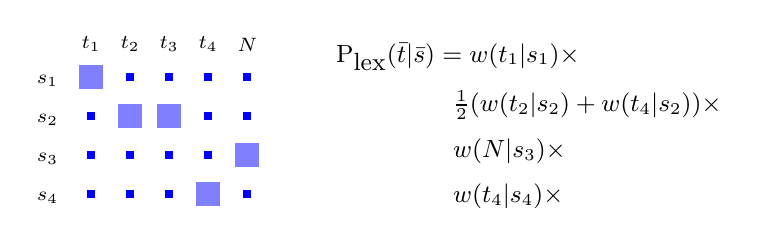
\begin{tikzpicture}

\tikzstyle{elementnode} = [rectangle,text=white,anchor=center]
\tikzstyle{srcnode} = [font=\small,anchor=south west]
\tikzstyle{tgtnode} = [left,font=\small,anchor=north east]
\tikzstyle{alignmentnode} = [rectangle,draw,minimum height=3.6*1.1cm,minimum width=0.36*1.1cm]
\tikzstyle{probnode} = [fill=blue!30,minimum width=0.4*1.1cm]
\tikzstyle{labelnode} = [above]

% alignment matrix1
\begin{scope}[scale=0.9,yshift=0.12in]
\foreach \i / \j / \c in
    {0/3/0.15, 1/3/0.15, 2/3/0.15, 3/3/0.15, 4/3/0.15,
    0/2/0.15, 1/2/0.15, 2/2/0.15, 3/2/0.15, 4/2/0.15,
    0/1/0.15, 1/1/0.15, 2/1/0.15, 3/1/0.15, 4/1/0.15,
    0/0/0.15, 1/0/0.15, 2/0/0.15, 3/0/0.15, 4/0/0.15}
    \node[elementnode,minimum size=0.6*1.1cm*\c,inner sep=0.1pt,fill=blue] (a\i\j) at (0.5*1.1cm*\i-5.4*0.5*1.1cm,0.5*1.1cm*\j-1.05*1.1cm) {};

% source
\node[srcnode] (tgt01) at (-5.9*0.5*1.1cm,-1.05*1.1cm+3.4*0.5*1.1cm) {\scriptsize{$t_1$}};
\node[srcnode] (tgt02) at ([xshift=0.5*1.1cm]tgt01.south west) {\scriptsize{$t_2$}};
\node[srcnode] (tgt03) at ([xshift=0.5*1.1cm]tgt02.south west) {\scriptsize{$t_3$}};
\node[srcnode] (tgt04) at ([xshift=0.5*1.1cm]tgt03.south west) {\scriptsize{$t_4$}};
\node[srcnode] (tgt05) at ([xshift=0.5*1.1cm]tgt04.south west) {\scriptsize{$N$}};

% target
\node[tgtnode] (src01) at (-6.0*0.5*1.1cm,-1.05*1.1cm+3.3*0.5*1.1cm) {\scriptsize{$s_1$}};
\node[tgtnode] (src02) at ([yshift=-0.5*1.1cm]src01.north east) {\scriptsize{$s_2$}};
\node[tgtnode] (src03) at ([yshift=-0.5*1.1cm]src02.north east) {\scriptsize{$s_3$}};
\node[tgtnode] (src04) at ([yshift=-0.5*1.1cm]src03.north east) {\scriptsize{$s_4$}};

% word alignment
\node[align=center,elementnode,minimum size=0.3cm,inner sep=0.1pt,fill=blue!50] (la1) at (a03) {};
\node[align=center,elementnode,minimum size=0.3cm,inner sep=0.1pt,fill=blue!50] (la2) at (a12) {};
\node[align=center,elementnode,minimum size=0.3cm,inner sep=0.1pt,fill=blue!50] (la3) at (a22) {};
\node[align=center,elementnode,minimum size=0.3cm,inner sep=0.1pt,fill=blue!50] (la4) at (a41) {};
\node[align=center,elementnode,minimum size=0.3cm,inner sep=0.1pt,fill=blue!50] (la5) at (a30) {};

\node[anchor=west] (f1) at ([xshift=3em,yshift=0.8em]a43.east) {\small{$\textrm{P}_{\textrm{lex}}(\bar{t}|\bar{s})=w(t_1|s_1)\times$}};
\node[anchor=north] (f2) at ([xshift=5.2em]f1.south) {\small{$\frac{1}{2}(w(t_2|s_2)+w(t_4|s_2))\times$}};
\node[anchor=north west] (f3) at (f2.south west) {\small{$w(N|s_3)\times$}};
\node[anchor=north west] (f4) at (f3.south west) {\small{$w(t_4|s_4)\times$}};

\end{scope}

\end{tikzpicture}
\end{center}
\caption{词汇翻译概率实例}
\label{fig:4-17}
\end{figure}
%-------------------------------------------

\parinterval 下面来看一个具体的例子,如图\ref{fig:4-17}所示。对于一个双语短语,将它们的词对齐关系代入到上面的公式就会得到短语的词汇翻译概率。对于词汇翻译概率,可以使用IBM 模型中的单词翻译表,也可以通过统计获得\cite{koehn2002learning}。如果一个单词的词对齐为空,则用$N$表示它翻译为空的概率。和短语翻译概率一样,可以使用双向的词汇化翻译概率来评价双语短语的好坏。

%----------------------------------------------
\begin{figure}[htp]
\centering
%%%------------------------------------------------------------------------------------------------------------
%%% 展示短语表的内容
\begin{center}
\begin{tikzpicture}
\node [anchor=west] (s1) at (0,0) {\small{报告 认为 $\vert\vert\vert$ report holds that $\vert\vert\vert$ -2.62 -5.81 -0.91 -2.85 1 0 $\vert\vert\vert$ 4 $\vert\vert\vert$ 0-0 1-1 1-2}};
\node [anchor=west] (s2) at ([yshift=-1.2em]s1.west) {\small{,悲伤 $\vert\vert\vert$ , sadness $\vert\vert\vert$ -1.946 -3.659 0 -3.709 1 0 $\vert\vert\vert$ 1 $\vert\vert\vert$ 0-0 1-1}};
\node [anchor=west] (s3) at ([yshift=-1.2em]s2.west) {\small{,北京 等 $\vert\vert\vert$ , beijing , and other $\vert\vert\vert$ 0 -7.98 0 -3.84 1 0 $\vert\vert\vert$ 2 $\vert\vert\vert$ 0-0 1-1 2-2 2-3 2-4}};
\node [anchor=west] (s4) at ([yshift=-1.2em]s3.west) {\small{,北京 及 $\vert\vert\vert$ , beijing , and $\vert\vert\vert$ -0.69 -1.45 -0.92 -4.80 1 0  $\vert\vert\vert$ 2 $\vert\vert\vert$ 0-0 1-1 2-2}};
\node [anchor=west] (s5) at ([yshift=-1.2em]s4.west) {\small{一个 中国 $\vert\vert\vert$ one china $\vert\vert\vert$ 0 -1.725 0 -1.636 1 0 $\vert\vert\vert$ 2 $\vert\vert\vert$ 1-1 2-2}};
\node [anchor=west] (s7) at ([yshift=-1.1em]s5.west) {\small{...}};
\node [anchor=west] (s6) at ([yshift=1.0em]s1.west) {\small{...}};
\begin{pgfonlayer}{background}
\node [rectangle,inner sep=0.3em,fill=red!10] [fit = (s1) (s3) (s4) (s6) (s7)] (box1) {};
\end{pgfonlayer}
\end{tikzpicture}
\end{center}
\caption{短语表实例}
\label{fig:4-18}
\end{figure}
%-------------------------------------------

\parinterval 经过上面的介绍,可以从双语平行语料中把双语短语抽取出来,同时得到相应的翻译概率(即特征),组成{\small\bfnew{短语表}}\index{短语表}(Phrase Table)\index{Phrase Table}。图\ref{fig:4-18}展示了一个真实短语表的片段。其中包括源语言短语和目标语言短语,用|||进行分割。每个双语对应的得分,包括正向和反向的词汇翻译概率以及短语翻译概率,还包括词对齐信息(0-0、1-1)等其他信息。

%----------------------------------------------------------------------------------------
%    NEW SUB-SECTION
%----------------------------------------------------------------------------------------

\subsection{调序}\label{subsection-4.2.4}

\parinterval 尽管已经知道了如何将一个源语言短语翻译成目标语言短语,但是想要获得一个高质量的译文,仅有互译的双语短语是远远不够的。

%----------------------------------------------
\begin{figure}[htp]
\centering
%%%------------------------------------------------------------------------------------------------------------
%%% 调序模型1:基于距离的调序
\begin{center}
\begin{tikzpicture}

\begin{scope}[minimum height = 20pt]

\node[anchor=east] (s0) at (-0.5em, 0) {$\textbf{s}$:};
\node[anchor=west,fill=green!20] (s1) at (0, 0) {\footnotesize{在 桌子 上 的}};
\node[anchor=west,fill=red!20] (s2) at ([xshift=1em]s1.east) {\footnotesize{苹果}};

\node[anchor=east] (t0) at (-0.5em, -1.5) {$\textbf{t}$:};
\node[anchor=west,fill=red!20] (t1) at (0, -1.5) {\footnotesize{the apple}};
\node[anchor=west,fill=green!20] (t2) at ([xshift=1em]t1.east) {\footnotesize{on the table}};

\path[<->, thick] (s1.south) edge (t2.north);
\path[<->, thick] (s2.south) edge (t1.north);

\end{scope}
\end{tikzpicture}
\end{center}
\caption{基于短语翻译的调序}
\label{fig:4-19}
\end{figure}
%-------------------------------------------

\parinterval 如图\ref{fig:4-19}所示,按照从左到右的顺序对一个句子``在\ \ 桌子\ \ 上\ \ 的\ \ 苹果''进行翻译,得到的译文``on the table the apple''的语序是不对的。虽然可以使用$n$-gram语言模型对语序进行建模,但是此处仍然需要用更加准确的方式描述目标语短语间的次序。一般,把这个问题称为短语调序,或者简称{\small\bfnew{调序}}\index{调序}(Reordering)\index{Reordering}。通常,基于短语的调序模型会作为判别式模型的特征参与到翻译过程中来。接下来,会介绍3 种不同的调序方法,分别是基于距离的调序、基于方向的调序(MSD模型)以及基于分类的调序。

%----------------------------------------------------------------------------------------
%    NEW SUBSUB-SECTION
%----------------------------------------------------------------------------------------

\subsubsection{基于距离的调序}

\parinterval 基于距离的调序是最简单的一种调序模型。很多时候,语言的翻译基本上都是顺序的,也就是,译文单词出现的顺序和源语言单词的顺序基本上是一致的。反过来说,如果译文和源语言单词(或短语)的顺序差别很大,就认为出现了调序。

\parinterval 基于距离的调序方法的核心思想就是度量当前翻译结果与顺序翻译之间的差距。对于译文中的第$i$个短语,令$start_i$表示它所对应的源语言短语中第一个词所在的位置,$end_i$表示它所对应的源语言短语中最后一个词所在的位置。于是,这个短语(相对于前一个短语)的调序距离为:
\begin{eqnarray}
dr = start_i-end_{i-1}-1
\label{eq:4-15}
\end{eqnarray}

\parinterval 在图\ref{fig:4-20}的例子中,``the apple''所对应的调序距离为4,``on the table''所对应的调序距离为-5。显然,如果两个源语短语按顺序翻译,则$start_i = end_{i-1} + 1$,这时调序距离为0。

%----------------------------------------------
\begin{figure}[htp]
\centering
%%%------------------------------------------------------------------------------------------------------------
%%% 调序模型1:基于距离的调序
\begin{center}
\begin{tikzpicture}

\begin{scope}[minimum height = 20pt]

\node[anchor=east] (s0) at (-0.5em, 0) {$\textbf{s}$:};
\node[anchor=west,fill=green!20] (s1) at (0, 0) {\small{在\ \ 桌子\ \ 上\ \ \;的}};
\node[anchor=south] (n1) at ([xshift=-2.5em,yshift=-0.5em]s1.north) {\small{1}};
\node[anchor=south] (n2) at ([xshift=-0.7em,yshift=-0.5em]s1.north) {\small{2}};
\node[anchor=south] (n3) at ([xshift=1.2em,yshift=-0.5em]s1.north) {\small{3}};
\node[anchor=south] (n4) at ([xshift=2.7em,yshift=-0.5em]s1.north) {\small{4}};
\node[anchor=west,fill=red!20] (s2) at ([xshift=1em]s1.east) {\small{苹果}};
\node[anchor=south] (n5) at ([yshift=-0.5em]s2.north) {\small{5}};

\node[anchor=east] (t0) at (-0.5em, -1.5) {$\textbf{t}$:};
\node[anchor=west,fill=red!20] (t1) at (0, -1.5) {\small{the apple}};
\node[anchor=west,fill=green!20] (t2) at ([xshift=1.3em]t1.east) {\small{on the table}};

\path[<->, thick] (s1.south) edge (t2.north);
\path[<->, thick] (s2.south) edge (t1.north);

\node[anchor=west] (target) at ([xshift=2em,yshift=2.3em]n5.east) {\small{目标短语位置}};
\node[anchor=west] (source) at ([xshift=0.3em]target.east) {\small{源短语位置}};
\node[anchor=west] (distance) at ([xshift=1.5em]source.east) {\small{距离}};

\node[anchor=north] (t1) at ([xshift=0em,yshift=-0.1em]target.south) {1};
\node[anchor=north] (t2) at ([yshift=-1.8em]t1.south) {2};

\node[anchor=north] (so1) at ([yshift=-0.1em]source.south) {5};
\node[anchor=north] (so2) at ([yshift=-1.8em]so1.south) {1-4};

\node[anchor=north] (d1) at ([xshift=-0.1em,yshift=-0.1em]distance.south) {+4};
\node[anchor=north] (d2) at ([yshift=-1.8em]d1.south) {-5};

\node[anchor=north west,fill=blue!20] (m1) at ([xshift=-1em,yshift=-0.0em]t1.south west) {\small{$start_1\ \ -\ \ end_{0}\ \ -\ \ 1$\quad =\quad 5\ -\ 0\ -\ 1}};
\node[anchor=north west,fill=blue!20] (m2) at ([xshift=-1em,yshift=-0.0em]t2.south west) {\small{$start_2\ \ -\ \  end_{1}\ \ -\ \ 1$\quad =\quad 1\ -\ 5\ -\ 1}};

\draw[-] ([xshift=0.08in]target.south west)--([xshift=2.4in]target.south west);

\draw[-,thick] (s1.north west)--([yshift=0.3in]s1.north west);
\draw[->,densely dotted,thick] ([yshift=0.3in]s1.north west)--([xshift=0.3in,yshift=0.3in]s1.north west);

\draw[-,thick] (s2.north west)--([yshift=0.3in]s2.north west);
\draw[->,densely dotted,thick] ([yshift=0.3in]s2.north west)--([xshift=-0.3in,yshift=0.3in]s2.north west);

\node[anchor=south] (ld1) at ([xshift=-0.5em,yshift=0.4em]n1.north) {\small{$dr= -5$}};
\node[anchor=south] (ld2) at ([xshift=6.5em,yshift=0.4em]n1.north) {\small{$dr= +4$}};


\end{scope}
\end{tikzpicture}
\end{center}
\caption{基于距离的调序}
\label{fig:4-20}
\end{figure}
%-------------------------------------------

\parinterval 如果把调序距离作为特征,一般会使用指数函数$f(dr) = a^{|dr|}$作为特征函数(或者调序代价的函数),其中$a$是一个参数,控制调序距离对整个特征值的影响。调序距离$dr$的绝对值越大,调序代价越高。基于距离的调序模型比较适用于像法–英翻译这样的任务,因为两种语言的语序基本上是一致的。但是,对于汉–日翻译,由于句子结构存在很大差异(日语是谓词后置,而汉语中谓词放在宾语前),使用基于距离的调序会带来一些问题。因此,具体应用时应该根据语言之间的差异性有选择的使用该模型。

%----------------------------------------------------------------------------------------
%    NEW SUBSUB-SECTION
%----------------------------------------------------------------------------------------

\subsubsection{基于方向的调序}

\parinterval 基于方向的调序模型是另一种常用的调序模型。该模型是一种典型的词汇化调序模型,因此调序的结果会根据不同短语有所不同。简单来说,在目标语言端连续的情况下,该模型会判断两个双语短语在源语言端的调序情况,包含三种调序类型:顺序的单调翻译(M)、与前一个短语交换位置(S)、非连续翻译(D)。因此,这个模型也被称作MSD调序模型\cite{Gros2008MSD}。

%----------------------------------------------
\begin{figure}[htp]
\centering
%%%------------------------------------------------------------------------------------------------------------
%%% 调序模型2:MSD模型
\begin{center}
\begin{tikzpicture}

\tikzstyle{elementnode} = [rectangle,text=white,anchor=center]
\tikzstyle{srcnode} = [left,font=\small,anchor=south west]
\tikzstyle{tgtnode} = [left,font=\small,anchor=north east]
\tikzstyle{alignmentnode} = [rectangle,draw,minimum height=3.6*1.1cm,minimum width=0.36*1.1cm]
\tikzstyle{probnode} = [fill=blue!30,minimum width=0.4*1.1cm]
\tikzstyle{labelnode} = [above]

 alignment matrix
\begin{scope}[scale=0.92,yshift=0.12in]
\foreach \i / \j / \c in
    {0/5/0.15, 1/5/0.15, 2/5/0.15, 3/5/0.15, 4/5/0.15, 5/5/0.15, 6/5/0.15, 7/5/0.15,
    0/4/0.15, 1/4/0.15, 2/4/0.15, 3/4/0.15, 4/4/0.15, 5/4/0.15, 6/4/0.15, 7/4/0.15,
    0/3/0.15, 1/3/0.15, 2/3/0.15, 3/3/0.15, 4/3/0.15, 5/3/0.15, 6/3/0.15, 7/3/0.15,
    0/2/0.15, 1/2/0.15, 2/2/0.15, 3/2/0.15, 4/2/0.15, 5/2/0.15, 6/2/0.15, 7/2/0.15,
    0/1/0.15, 1/1/0.15, 2/1/0.15, 3/1/0.15, 4/1/0.15, 5/1/0.15, 6/1/0.15, 7/1/0.15,
    0/0/0.15, 1/0/0.15, 2/0/0.15, 3/0/0.15, 4/0/0.15, 5/0/0.15, 6/0/0.15, 7/0/0.15}
    \node[elementnode,minimum size=0.6*1.1cm*\c,inner sep=0.1pt,fill=blue] (a\i\j) at (0.5*1.1cm*\i-5.4*0.5*1.1cm,0.5*1.1cm*\j-0.05*1.1cm) {};

 source
\node[srcnode] (src1) at (-5.9*0.5*1.1cm,-1.05*1.1cm+7.5*0.5*1.1cm) {\scriptsize{$t_1$}};
\node[srcnode] (src2) at ([xshift=0.5*1.1cm]src1.south west) {\scriptsize{$t_2$}};
\node[srcnode] (src3) at ([xshift=0.5*1.1cm]src2.south west) {\scriptsize{$t_3$}};
\node[srcnode] (src4) at ([xshift=0.5*1.1cm]src3.south west) {\scriptsize{$t_4$}};
\node[srcnode] (src5) at ([xshift=0.5*1.1cm]src4.south west) {\scriptsize{$t_5$}};
\node[srcnode] (src6) at ([xshift=0.5*1.1cm]src5.south west) {\scriptsize{$t_6$}};
\node[srcnode] (src7) at ([xshift=0.5*1.1cm]src6.south west) {\scriptsize{$t_7$}};
\node[srcnode] (src8) at ([xshift=0.5*1.1cm]src7.south west) {\scriptsize{$t_8$}};

 target
\node[tgtnode] (tgt1) at (-6.0*0.5*1.1cm,-1.05*1.1cm+7.5*0.5*1.1cm) {\scriptsize{$s_1$}};
\node[tgtnode] (tgt2) at ([yshift=-0.5*1.1cm]tgt1.north east) {\scriptsize{$s_2$}};
\node[tgtnode] (tgt3) at ([yshift=-0.5*1.1cm]tgt2.north east) {\scriptsize{$s_3$}};
\node[tgtnode] (tgt4) at ([yshift=-0.5*1.1cm]tgt3.north east) {\scriptsize{$s_4$}};
\node[tgtnode] (tgt5) at ([yshift=-0.5*1.1cm]tgt4.north east) {\scriptsize{$s_5$}};
\node[tgtnode] (tgt6) at ([yshift=-0.5*1.1cm]tgt5.north east) {\scriptsize{$s_6$}};

 word alignment
\node[align=center,elementnode,minimum size=0.3cm,inner sep=0.1pt,fill=blue!50] (l05) at (a05) {};
\node[align=center,elementnode,minimum size=0.3cm,inner sep=0.1pt,fill=blue!50] (l14) at (a14) {};
\node[align=center,elementnode,minimum size=0.3cm,inner sep=0.1pt,fill=blue!50] (l24) at (a24) {};
\node[align=center,elementnode,minimum size=0.3cm,inner sep=0.1pt,fill=blue!50] (l31) at (a31) {};
\node[align=center,elementnode,minimum size=0.3cm,inner sep=0.1pt,fill=blue!50] (l32) at (a32) {};
\node[align=center,elementnode,minimum size=0.3cm,inner sep=0.1pt,fill=blue!50] (l43) at (a43) {};
\node[align=center,elementnode,minimum size=0.3cm,inner sep=0.1pt,fill=blue!50] (l53) at (a53) {};
\node[align=center,elementnode,minimum size=0.3cm,inner sep=0.1pt,fill=blue!50] (l63) at (a63) {};
\node[align=center,elementnode,minimum size=0.3cm,inner sep=0.1pt,fill=blue!50] (l70) at (a70) {};


{
\node [anchor=west] (p1line1) at ([xshift=3.5em,yshift=0.5em]a75.east) {\footnotesize{M(monotone):单调调序}};
\node [anchor=north west] (p1line2) at ([xshift=0,yshift=-1em]p1line1.south west) {\footnotesize{S(swap): 与前面一个短语}};
\node [anchor=north west] (p1line3) at ([xshift=3.5em]p1line2.south west) {\footnotesize{位置进行交换}};
\node [anchor=north west] (p1line4) at ([xshift=-3.5em,yshift=-1em]p1line3.south west) {\footnotesize{D(discontinuous):非连续调序}};

\node [anchor=east] (p1line5) at ([xshift=0em,yshift=3em]p1line4.east) {};
\node [anchor=east] (p1line6) at ([xshift=0em,yshift=7em]p1line4.east) {};

%\node [anchor=west] (p2line1) at ([xshift=4em]a73.east) {\footnotesize{$\bar{s}_j$: 真\ \ \ 好 \ \ }};
%\node [anchor=north west] (p2line2) at ([xshift=0]p2line1.south west) {\footnotesize{$\bar{t}_j$: very\ \ \ good\ \ \ \ \ \ \ \ }};

\begin{pgfonlayer}{background}
{
\node [rectangle,thick,inner sep=0.3em,fill=blue!40,drop shadow,fill opacity=0.85] [fit = (a05)] (phrase1) {};
\node [rectangle,thick,inner sep=0.3em,fill=blue!40,drop shadow,fill opacity=0.85] [fit = (a14) (a24)] (phrase2) {};
\node [rectangle,thick,inner sep=0.3em,fill=blue!40,drop shadow,fill opacity=0.85] [fit = (a31) (a32)] (phrase3) {};
\node [rectangle,thick,inner sep=0.3em,fill=blue!40,drop shadow,fill opacity=0.85] [fit = (a43) (a63)] (phrase4) {};
\node [rectangle,thick,inner sep=0.3em,fill=blue!40,drop shadow,fill opacity=0.85] [fit = (a70)] (phrase5) {};
\node [rectangle,inner sep=0.2em,fill=red!10] [fit = (p1line1) (p1line6)] (box1) {};
\node [rectangle,inner sep=0.2em,fill=ugreen!10] [fit = (p1line2) (p1line3) (p1line5)] (box2) {};
\node [rectangle,inner sep=0.2em,fill=orange!10] [fit = (p1line4)] (box3) {};
}
\end{pgfonlayer}

\node [circle,draw,anchor=south,inner sep=1pt,fill=red!20] (c1) at ([xshift=-0.5em]a05.north) {\scriptsize{m}};
\node [circle,draw,anchor=south,inner sep=1pt,fill=red!20] (c2) at ([xshift=-0.5em]a14.north) {\scriptsize{m}};
\node [circle,draw,anchor=north,inner sep=1pt,fill=orange!20] (c3) at ([xshift=0.1em]a24.south) {\scriptsize{d}};
\node [circle,draw,anchor=south,inner sep=2pt,fill=ugreen!20] (c4) at ([xshift=0.5em]a32.north) {\scriptsize{s}};
\node [circle,draw,anchor=north,inner sep=1pt,fill=orange!20] (c5) at ([xshift=0.5em]a63.south) {\scriptsize{d}};


\draw [->,thick] (a05.south east) -- (c1.315);
\draw [->,thick] ([xshift=-0.5em]a24.west) -- (c2.315);
\draw [->,thick] ([yshift=-0.7em]a32.south) .. controls +(west:1.3) and +(east:1.3) .. (c3.340);
\draw [->,thick] (a53.center) -- (c4.15);
\draw [->,thick] (a70.center) .. controls +(west:1.3) and +(east:1.3) .. (c5.340);
}
\end{scope}

\end{tikzpicture}
\end{center}
\caption{词汇化调序模型的三种调序类型}
\label{fig:4-21}
\end{figure}
%-------------------------------------------

\parinterval 图\ref{fig:4-21}展示了这三种调序类型,当两个短语对在源语言和目标语言中都是按顺序排列时,它们就是单调的(如:从左边数前两个短语);如果对应的短语顺序在目标语中是反过来的,属于交换调序(如:从左边数第三和第四个短语);如果两个短语之间还有其他的短语,就是非连续翻译(如:从右边数的前两个短语)。

\parinterval 对于每种调序类型,都可以定义一个调序概率,如下:
\begin{eqnarray}
\textrm{P}(\mathbf{o}|\mathbf{s},\mathbf{t},\mathbf{a}) = \prod_{i=1}^{K} \textrm{P}(o_i| \bar{s}_{a_i}, \bar{t}_i, a_{i-1}, a_i)
\label{eq:4-16}
\end{eqnarray}

\noindent 其中,$o_i$表示(目标语言)第$i$个短语的调序方向,$\mathbf{o}=\{o_i\}$表示短语序列的调序方向,$K$表示短语的数量。短语之间的调序概率是由双语短语以及短语对齐决定的,$o$表示调序的种类,可以取M、S、D 中的任意一种。而整个句子调序的好坏就是把相邻的短语之间的调序概率相乘(对应取log后的加法)。这样,公式\ref{eq:4-16}把调序的好坏定义为新的特征,对于M、S、D总共就有三个特征。除了当前短语和前一个短语的调序特征,还可以定义当前短语和后一个短语的调序特征,即将上述公式中的$a_{i-1}$换成$a_{i+1}$。 于是,又可以得到三个特征。因此在MSD调序中总共可以有6个特征。

%----------------------------------------------
\begin{figure}[htp]
\centering
%------------------------------------------------------------------------------------------------------------
%%% 调序模型2:MSD模型
\begin{center}
\begin{tikzpicture}
\tikzstyle{elementnode} = [rectangle,anchor=center]
\tikzstyle{srcnode} = [font=\small,anchor=south west]
\tikzstyle{tgtnode} = [left,font=\small,anchor=north east]
\tikzstyle{alignmentnode} = [rectangle,draw,minimum height=3.6*1.1cm,minimum width=0.36*1.1cm]
\tikzstyle{probnode} = [fill=blue!30,minimum width=0.4*1.1cm]
\tikzstyle{labelnode} = [above]

% alignment matrix1
\begin{scope}[scale=0.9,yshift=0.12in]
\foreach \i / \j / \c in
    {0/5/0.15, 1/5/0.15, 2/5/0.15, 3/5/0.15, 4/5/0.15, 5/5/0.15,
    0/4/0.15, 1/4/0.15, 2/4/0.15, 3/4/0.15, 4/4/0.15, 5/4/0.15,
    0/3/0.15, 1/3/0.15, 2/3/0.15, 3/3/0.15, 4/3/0.15, 5/3/0.15,
    0/2/0.15, 1/2/0.15, 2/2/0.15, 3/2/0.15, 4/2/0.15, 5/2/0.15,
    0/1/0.15, 1/1/0.15, 2/1/0.15, 3/1/0.15, 4/1/0.15, 5/1/0.15,
    0/0/0.15, 1/0/0.15, 2/0/0.15, 3/0/0.15, 4/0/0.15, 5/0/0.15}
    \node[elementnode,minimum size=0.6*1.1cm*\c,inner sep=0.1pt,fill=blue] (a\i\j) at (0.5*1.1cm*\i-5.4*0.5*1.1cm,0.5*1.1cm*\j-1.05*1.1cm) {};

% source
\node[srcnode] (src01) at (-5.9*0.5*1.1cm,-1.05*1.1cm+5.4*0.5*1.1cm) {\scriptsize{$t_1$}};
\node[srcnode] (src02) at ([xshift=0.5*1.1cm]src01.south west) {\scriptsize{$t_2$}};
\node[srcnode] (src03) at ([xshift=0.5*1.1cm]src02.south west) {\scriptsize{$t_3$}};
\node[srcnode] (src04) at ([xshift=0.5*1.1cm]src03.south west) {\scriptsize{$t_4$}};
\node[srcnode] (src05) at ([xshift=0.5*1.1cm]src04.south west) {\scriptsize{$t_5$}};
\node[srcnode] (src06) at ([xshift=0.5*1.1cm]src05.south west) {\scriptsize{$t_6$}};

% target
\node[tgtnode] (tgt01) at (-6.0*0.5*1.1cm,-1.05*1.1cm+5.4*0.5*1.1cm) {\scriptsize{$s_1$}};
\node[tgtnode] (tgt02) at ([yshift=-0.5*1.1cm]tgt01.north east) {\scriptsize{$s_2$}};
\node[tgtnode] (tgt03) at ([yshift=-0.5*1.1cm]tgt02.north east) {\scriptsize{$s_3$}};
\node[tgtnode] (tgt04) at ([yshift=-0.5*1.1cm]tgt03.north east) {\scriptsize{$s_4$}};
\node[tgtnode] (tgt05) at ([yshift=-0.5*1.1cm]tgt04.north east) {\scriptsize{$s_5$}};
\node[tgtnode] (tgt06) at ([yshift=-0.5*1.1cm]tgt05.north east) {\scriptsize{$s_6$}};

%% alignment matrix2
\foreach \i / \j / \c in
    {0/5/0.15, 1/5/0.15, 2/5/0.15, 3/5/0.15, 4/5/0.15, 5/5/0.15,
    0/4/0.15, 1/4/0.15, 2/4/0.15, 3/4/0.15, 4/4/0.15, 5/4/0.15,
    0/3/0.15, 1/3/0.15, 2/3/0.15, 3/3/0.15, 4/3/0.15, 5/3/0.15,
    0/2/0.15, 1/2/0.15, 2/2/0.15, 3/2/0.15, 4/2/0.15, 5/2/0.15,
    0/1/0.15, 1/1/0.15, 2/1/0.15, 3/1/0.15, 4/1/0.15, 5/1/0.15,
    0/0/0.15, 1/0/0.15, 2/0/0.15, 3/0/0.15, 4/0/0.15, 5/0/0.15}
    \node[elementnode,minimum size=0.6*1.1cm*\c,inner sep=0.1pt,fill=blue] (b\i\j) at (0.5*1.1cm*\i+4*0.5*1.1cm,0.5*1.1cm*\j-1.05*1.1cm) {};

% source
\node[srcnode] (src11) at (3.5*0.5*1.1cm,-1.05*1.1cm+5.4*0.5*1.1cm) {\scriptsize{$t_1$}};
\node[srcnode] (src12) at ([xshift=0.5*1.1cm]src11.south west) {\scriptsize{$t_2$}};
\node[srcnode] (src13) at ([xshift=0.5*1.1cm]src12.south west) {\scriptsize{$t_3$}};
\node[srcnode] (src14) at ([xshift=0.5*1.1cm]src13.south west) {\scriptsize{$t_4$}};
\node[srcnode] (src15) at ([xshift=0.5*1.1cm]src14.south west) {\scriptsize{$t_5$}};
\node[srcnode] (src16) at ([xshift=0.5*1.1cm]src15.south west) {\scriptsize{$t_6$}};

% target
\node[tgtnode] (tgt11) at (3.4*0.5*1.1cm,-1.05*1.1cm+5.4*0.5*1.1cm) {\scriptsize{$s_1$}};
\node[tgtnode] (tgt12) at ([yshift=-0.5*1.1cm]tgt11.north east) {\scriptsize{$s_2$}};
\node[tgtnode] (tgt13) at ([yshift=-0.5*1.1cm]tgt12.north east) {\scriptsize{$s_3$}};
\node[tgtnode] (tgt14) at ([yshift=-0.5*1.1cm]tgt13.north east) {\scriptsize{$s_4$}};
\node[tgtnode] (tgt15) at ([yshift=-0.5*1.1cm]tgt14.north east) {\scriptsize{$s_5$}};
\node[tgtnode] (tgt16) at ([yshift=-0.5*1.1cm]tgt15.north east) {\scriptsize{$s_6$}};


% word alignment
\node[align=center,elementnode,minimum size=0.3cm,inner sep=0.1pt,fill=blue!50] (la1) at (a23) {};
\node[align=center,elementnode,minimum size=0.3cm,inner sep=0.1pt,fill=blue!50] (la2) at (a22) {};
\node[align=center,elementnode,minimum size=0.3cm,inner sep=0.1pt,fill=blue!50] (la3) at (a31) {};
{
\node[align=center,elementnode,minimum size=0.5cm,inner sep=0.1pt,fill=red!50] (la4) at (a14) {M};
}

{
\node[align=center,elementnode,minimum size=0.5cm,inner sep=0.1pt,fill=ugreen!50] (la5) at (a44) {S};
}

\node[align=center,elementnode,minimum size=0.3cm,inner sep=0.1pt,fill=blue!50] (lb1) at (b23) {};
\node[align=center,elementnode,minimum size=0.3cm,inner sep=0.1pt,fill=blue!50] (lb2) at (b22) {};
\node[align=center,elementnode,minimum size=0.3cm,inner sep=0.1pt,fill=blue!50] (lb3) at (b31) {};
{
\node[align=center,elementnode,minimum size=0.3cm,inner sep=0.1pt,fill=red!50] (lb4) at (b05) {};
\node[align=center,elementnode,minimum size=0.3cm,inner sep=0.1pt,fill=red!50] (lb5) at (b14) {};
}
{
\node[align=center,elementnode,minimum size=0.3cm,inner sep=0.1pt,fill=ugreen!50] (lb6) at (b45) {};
\node[align=center,elementnode,minimum size=0.3cm,inner sep=0.1pt,fill=ugreen!50] (lb7) at (b54) {};
}

\begin{pgfonlayer}{background}
\node [rectangle,thick,inner sep=0.4em,fill=blue!40,drop shadow,fill opacity=0.85] [fit = (a23) (a31)] (phrase1) {};
\node [rectangle,thick,inner sep=0.4em,fill=blue!40,drop shadow,fill opacity=0.85] [fit = (b23) (b31)] (phrase2) {};
{
\node [rectangle,thick,inner sep=0.4em,fill=red!40,drop shadow,fill opacity=0.85] [fit = (b05) (b14)] (phrase3) {};
}
{
\node [rectangle,thick,inner sep=0.4em,fill=ugreen!40,drop shadow,fill opacity=0.85] [fit = (b45) (b54)] (phrase4) {};
}
\end{pgfonlayer}

{
\node[anchor=north] (s1) at ([xshift=0.6em,yshift=0.1em]b45.east) {S};
}
{
\node[anchor=north] (m1) at ([xshift=0.6em,yshift=0.1em]b05.east) {M};
}

\node[anchor=north] (l1) at ([xshift=1.8em,yshift=-0.5em]a10.south) {\scriptsize{基于词}};
\node[anchor=north] (l2) at ([xshift=2.2em,yshift=-0.5em]b10.south) {\scriptsize{基于短语}};

\end{scope}

\end{tikzpicture}
\end{center}
\caption{调序类型的判断}
\label{fig:4-22}
\end{figure}
%-------------------------------------------

\parinterval 具体实现时,通常使用词对齐对两个短语间的调序关系进行判断。图\ref{fig:4-22}展示了这个过程。先判断短语的左上角和右上角是否存在词对齐,再根据其位置对调序类型进行划分。每个短语对应的调序概率都可以用相对频率估计进行计算。而MSD调序模型也相当于在短语表中的每个双语短语后添加6个特征。不过,调序模型一般并不会和短语表一起存储,因此在系统中通常会看到两个独立的模型文件,分别保存短语表和调序模型。

%----------------------------------------------------------------------------------------
%    NEW SUBSUB-SECTION
%----------------------------------------------------------------------------------------

\subsubsection{基于分类的调序}

\parinterval 在MSD调序中,双语短语所对应的调序概率$\textrm{P}(o_i| \bar{s}_{a_i}, \bar{t}_i, a_{i-1}, a_i)$是用极大似然估计方法进行计算的。但是,这种方法也会面临数据稀疏问题,同时对调序产生影响的细致特征也没有考虑进来。另一种有效的方法是直接用统计分类模型对调序进行建模,比如,可以使用最大熵、SVM等分类器输出调序概率或者得分\cite{xiong2006maximum,DBLP:journals/coling/OchN04,DBLP:conf/naacl/KumarB05}。对于基于分类的调序模型,有两方面问题需要考虑:

\begin{itemize}
\vspace{0.5em}
\item 训练样本的生成。可以把M、S、D看作是类别标签,把所对应的短语及短语对齐信息看作是输入。这样就得到了大量分类器训练所需的样本;
\vspace{0.5em}
\item 分类特征设计。这部分是传统统计机器学习中的重要组成部分,好的特征会对分类结果产生很大影响。在调序模型中,一般直接使用单词作为特征,比如用短语的第一个单词和最后一个单词作为特征就可以达到很好的效果。
\vspace{0.5em}
\end{itemize}

\parinterval 随着神经网络方法的兴起,也可以考虑使用多层神经网络构建调序模型\cite{li-etal-2014-neural}。这时,可以把短语直接送入一个神经网络,之后由神经网络完成对特征的抽取和表示,并输出最终的调序模型得分。

%----------------------------------------------------------------------------------------
%    NEW SUB-SECTION
%----------------------------------------------------------------------------------------

\subsection{特征}

\parinterval 基于短语的模型使用判别式模型对翻译推导进行建模,给定双语句对$(\mathbf{s},\mathbf{t})$,每个翻译推导$d$都有一个模型得分,由$M$个特征线性加权得到,记为$\textrm{score}(d,\mathbf{t},\mathbf{s}) = \sum_{i=1}^{M} \lambda_i \cdot h_i (d,\mathbf{t},\mathbf{s})$,其中$\lambda_i$表示特征权重,$h_i (d,\mathbf{t},\mathbf{s})$表示特征函数(简记为$h_i (d)$)。这些特征包含刚刚介绍过的短语翻译概率、调序模型得分等,除此之外,还包含语言模型等其他特征,它们共同组成了特征集合。这里列出了基于短语的模型中常用的特征:

\begin{itemize}
\vspace{0.5em}
\item 短语翻译概率(取对数),包含正向翻译概率$\textrm{log}(\textrm{P}(\bar{t}|\bar{s}))$和反向翻译概率$\textrm{log}(\textrm{P}(\bar{s}$\\$|\bar{t}))$,它们是基于短语的模型中最主要的特征;
\vspace{0.5em}
\item 词汇化翻译概率(取对数),同样包含正向词汇化翻译概率$\textrm{log(P}_{\textrm{lex}}(\bar{t}|\bar{s}\textrm{))}$和反向词汇化翻译概率$\textrm{log(P}_{\textrm{lex}}(\bar{s}|\bar{t}\textrm{))}$,它们用来描述双语短语中单词间对应的好坏;
\vspace{0.5em}
\item $n$-gram语言模型,用来度量译文的流畅程度,可以通过大规模目标端单语数据得到;
\vspace{0.5em}
\item 译文长度,避免模型倾向于短译文,同时让系统自动学习对译文长度的偏好;
\vspace{0.5em}
\item 翻译规则数量,为了避免模型仅使用少量特征构成翻译推导(规则数量少,短语翻译概率相乘的因子也会少,得分一般会大一些),同时让系统自动学习对规则数量的偏好;
\vspace{0.5em}
\item 被翻译为空的源语言单词数量。注意,空翻译规则有时也被称作evil feature,这类特征在一些数据上对BLEU有很好的提升作用,但会造成人工评价结果的下降,需要谨慎使用;
\vspace{0.5em}
\item 基于MSD的调序模型,包括与前一个短语的调序模型$f_{\textrm{M-pre}}(d)$\ 、$f_{\textrm{S-pre}}(d)$\ 、$f_{\textrm{D-pre}}(d)$和与后一个短语的调序模型$f_{\textrm{M-fol}}(d)$\ 、$f_{\textrm{S-fol}}(d)$\ 、$f_{\textrm{D-fol}}(d)$,共6个特征。
\vspace{0.5em}
\end{itemize}

%----------------------------------------------------------------------------------------
%    NEW SUB-SECTION
%----------------------------------------------------------------------------------------

\subsection{最小错误率训练}\label{subsection-4.2.6}

\parinterval 除了特征设计,统计机器翻译也需要找到每个特征所对应的最优权重$\lambda_i$。这也就是机器学习中所说的模型训练问题。不过,需要指出的是,统计机器翻译关于模型训练的定义与传统机器学习稍有不同。在统计机器翻译中,短语抽取和翻译概率的估计被看作是{\small\bfnew{模型训练}}\index{模型训练}(Model Training)\index{Model Training},也就是说这里的模型训练是指特征函数的学习;而特征权重的训练,一般被称作{\small\bfnew{权重调优}}\index{权重调优}(Weight Tuning)\index{Weight Tuning},而这个过程才真正对应了传统机器学习(如分类任务)中的模型训练过程。在本章中,如果没有特殊说明,权重调优就是指特征权重的学习,模型训练是指短语抽取和特征函数的学习。

\parinterval 想要得到最优的特征权重,最简单的方法是枚举所有的特征权重可能的取值,然后评价每组权重所对应的翻译性能,最后选择最优的特征权重作为调优的结果。但是特征权重是一个实数值,因此可以考虑把实数权重进行量化,即把权重看作是在固定间隔上的取值,比如,每隔0.01取值。即使是这样,同时枚举多个特征的权重也是非常耗时的工作,当特征数量增多时这种方法的效率仍然很低。

\parinterval 这里介绍一种更加高效的特征权重调优方法$\ \dash \ ${\small\bfnew{最小错误率训练}}\index{最小错误率训练}(Minimum Error Rate Training\index{Minimum Error Rate Training},MERT)。最小错误率训练是统计机器翻译发展中代表性工作,也是从机器翻译中原创的重要技术方法之一\cite{och2003minimum}。最小错误率训练假设:翻译结果相对于标准答案的错误是可度量的,进而可以通过降低错误数量的方式来找到最优的特征权重。假设有样本集合$S = \{(s_1,\mathbf{r}_1),...,(s_N,\mathbf{r}_N)\}$,$s_i$为样本中第$i$个源语言句子,$\mathbf{r}_i$为相应的参考译文。注意,$\mathbf{r}_i$可以包含多个参考译文。$S$通常被称为{\small\bfnew{调优集合}}\index{调优集合}(Tuning Set)\index{Tuning Set}。对于$S$中的每个源语句子$s_i$,机器翻译模型会解码出$n$-best推导$d_{i}^{\ast} = \{\mathbf{d}_{ij}^{\ast}\}$,其中$d_{ij}^{\ast}$表示翻译源语言句子$s_i$时得到的第$j$个最好的推导。$\{d_{ij}^{\ast}\}$可以被定义如下:
\begin{eqnarray}
\{d_{ij}^{\ast}\} = \arg\max_{\{d_{ij}\}} \sum_{i=1}^{M} \lambda_i \cdot h_i (d,\mathbf{t},\mathbf{s})
\label{eq:4-17}
\end{eqnarray}

\parinterval 对于每个样本都可以得到$n$-best推导集合,整个数据集上的推导集合被记为$\mathbf{D}^{\ast} = \{\mathbf{d}_{1}^{\ast},...,\mathbf{d}_{s}^{\ast}\}$。进一步,令所有样本的参考译文集合为$\mathbf{R} = \{\mathbf{r}_1,...,\mathbf{r}_N\}$。最小错误率训练的目标就是降低$\mathbf{D}^{\ast}$相对于$\mathbf{R}$的错误。也就是,通过调整不同特征的权重$\lambda = \{ \lambda_i \}$,让错误率最小,形式化描述为:
\begin{eqnarray}
\lambda^{\ast} = \arg\min_{\lambda} \textrm{Error}(\mathbf{D}^{\ast},\mathbf{R})
\label{eq:4-18}
\end{eqnarray}
%公式--------------------------------------------------------------------

\noindent 其中\textrm{Error}$(\cdot)$是错误率函数。\textrm{Error}$(\cdot)$的定义方式有很多,一般来说\textrm{Error}$(\cdot)$会与机器翻译的评价指标相关,例如,词错误率(WER)、位置错误率(PER)、BLEU 值、NIST值等都可以用于\textrm{Error}$(\cdot)$的定义。这里使用1-BLEU作为错误率函数,即$\textrm{Error}(\mathbf{D}^{\ast},\mathbf{R}) = 1 - \textrm{BLEU}(\mathbf{D}^{\ast},\mathbf{R})$。则公式\ref{eq:4-18}可改写为:
%公式--------------------------------------------------------------------
\begin{eqnarray}
\lambda^{\ast} &=& \arg\min_{\lambda}\ 1 - \textrm{BLEU}(\mathbf{D}^{\ast},\mathbf{R})   \nonumber \\
&=& \arg\max_{\lambda} \textrm{BLEU}(\mathbf{D}^{\ast},\mathbf{R})
\label{eq:4-19}
\end{eqnarray}
%公式--------------------------------------------------------------------

\parinterval 需要注意的是, BLEU本身是一个不可微分函数。因此,无法使用梯度下降等方法对式\ref{eq:4-19}进行求解。那么如何能快速得到最优解?这里会使用一种特殊的优化方法,称作{\small\bfnew{线搜索}}\index{线搜索}(Line Search)\index{Line Search},它是Powell搜索的一种形式\cite{powell1964an}。这种方法也构成了最小错误率训练的核心。

\parinterval 首先,重新看一下特征权重的搜索空间。按照前面的介绍,如果要进行暴力搜索,需要把特征权重的取值按小的间隔进行划分。这样,所有特征权重的取值可以用图\ref{fig:4-23}的网格来表示。

%----------------------------------------------
\begin{figure}[htp]
\centering
\begin{tabular}{l l l}
& \subfigure{\begin{tikzpicture}
\begin{scope}[scale=0.55] 
{\tiny
\draw[step=1,help lines,color=black] grid (4,4); 

\node[anchor=north] (y2) at ([xshift=-3.3em,yshift=0em]n1.north) {0.01};
\node[anchor=north] (y1) at ([xshift=0em,yshift=-3.3em]y2.south) {0.00};
\node[anchor=north] (y3) at ([xshift=0em,yshift=4.5em]y2.north) {0.02};
\node[anchor=north] (y4) at ([xshift=0em,yshift=6.6em]y3.north) {$\vdots$};
\node[anchor=north] (y5) at ([xshift=0em,yshift=2em]y4.north) {1.00};

\node[anchor=north] (x1) at ([xshift=2em,yshift=-3em]n1.south) {$\lambda_1$};
\node[anchor=north] (x2) at ([xshift=4.5em,yshift=0em]x1.north) {$\lambda_2$};
\node[anchor=north] (x3) at ([xshift=4em,yshift=-1em]x2.north) {$...$};
\node[anchor=north] (x4) at ([xshift=5em,yshift=1em]x3.north) {$\lambda_{M-1}$};
\node[anchor=north] (x5) at ([xshift=5em,yshift=0em]x4.north) {$\lambda_M$};

\draw [-](n1) (0,4) -- (0,4.4);
\draw [-](n2) (1,4) -- (1,4.4);
\draw [-](n3) (2,4) -- (2,4.4);
\draw [-](n4) (3,4) -- (3,4.4);
\draw [-](n5) (4,4) -- (4,4.4);

\draw[decorate,decoration={brace}](0,4.7) --(4,4.7) node [xshift=-4em,yshift=1.5em,align=center](label1) {M dimensions};	

\draw[decorate,decoration={brace}](4.5,4.3) --(4.5,0) node [xshift=2.3em,yshift=5.8em,align=center](label2) {Values};	
}
\end{scope}
\end{tikzpicture}} \subfigure{\begin{tikzpicture}
\begin{scope}[scale=0.55] 
{\tiny
\draw[step=1,help lines,color=black] grid (4,4); 

\node[anchor=north] (y2) at ([xshift=-3.3em,yshift=0em]n1.north) {0.01};
\node[anchor=north] (y1) at ([xshift=0em,yshift=-3.3em]y2.south) {0.00};
\node[anchor=north] (y3) at ([xshift=0em,yshift=4.5em]y2.north) {0.02};
\node[anchor=north] (y4) at ([xshift=0em,yshift=6.6em]y3.north) {$\vdots$};
\node[anchor=north] (y5) at ([xshift=0em,yshift=2em]y4.north) {1.00};

\node[anchor=north] (x1) at ([xshift=2em,yshift=-3em]n1.south) {$\lambda_1$};
\node[anchor=north] (x2) at ([xshift=4.5em,yshift=0em]x1.north) {$\lambda_2$};
\node[anchor=north] (x3) at ([xshift=4em,yshift=-1em]x2.north) {$...$};
\node[anchor=north] (x4) at ([xshift=5em,yshift=1em]x3.north) {$\lambda_{M-1}$};
\node[anchor=north] (x5) at ([xshift=5em,yshift=0em]x4.north) {$\lambda_M$};

\draw [-](n1) (0,4) -- (0,4.4);
\draw [-](n2) (1,4) -- (1,4.4);
\draw [-](n3) (2,4) -- (2,4.4);
\draw [-](n4) (3,4) -- (3,4.4);
\draw [-](n5) (4,4) -- (4,4.4);

\node [anchor=center,draw,circle,inner sep=1.5pt,blue!30,fill=blue!30] (r11) at (0,1) {};
\node [anchor=center,draw,circle,inner sep=1.5pt,blue!30,fill=blue!30] (r12) at (1,2) {};
\node [anchor=center,draw,circle,inner sep=1.5pt,blue!30,fill=blue!30] (r13) at (2,1) {};
\node [anchor=center,draw,circle,inner sep=1.5pt,blue!30,fill=blue!30] (r14) at (3,2) {};
\node [anchor=center,draw,circle,inner sep=1.5pt,blue!30,fill=blue!30] (r15) at (4,4) {};

\draw [-,very thick,blue!50] (0,1) -- (1,2) -- (2,1) -- (3,2) -- (4,4);

\node[anchor=north] (p1) at ([xshift=5em,yshift=13em]n5.north) {\scriptsize{$\leftarrow$ \textbf{path}:}};

\node[anchor=north] (e1) at ([xshift=0,yshift=-0.4em]p1.south) {$w_1 = 0.01$};
\node[anchor=north] (e2) at ([xshift=0,yshift=-0.8em]e1.south) {$w_2 = 0.02$};
\node[anchor=north] (e3) at ([xshift=0,yshift=0.4em]e2.south) {$\vdots$};
\node[anchor=north] (e4) at ([xshift=0,yshift=-0.2em]e3.south) {$w_M = 1.00$};
}
\end{scope}
\end{tikzpicture}} \subfigure{\begin{tikzpicture}
\begin{scope}[scale=0.55] 
{\tiny
\draw[step=1,help lines,color=black] grid (4,4); 

\node[anchor=north] (y2) at ([xshift=-3.3em,yshift=0em]n1.north) {0.01};
\node[anchor=north] (y1) at ([xshift=0em,yshift=-3.3em]y2.south) {0.00};
\node[anchor=north] (y3) at ([xshift=0em,yshift=4.5em]y2.north) {0.02};
\node[anchor=north] (y4) at ([xshift=0em,yshift=6.6em]y3.north) {$\vdots$};
\node[anchor=north] (y5) at ([xshift=0em,yshift=2em]y4.north) {1.00};

\node[anchor=north] (x1) at ([xshift=2em,yshift=-3em]n1.south) {$\lambda_1$};
\node[anchor=north] (x2) at ([xshift=4.5em,yshift=0em]x1.north) {$\lambda_2$};
\node[anchor=north] (x3) at ([xshift=4em,yshift=-1em]x2.north) {$...$};
\node[anchor=north] (x4) at ([xshift=5em,yshift=1em]x3.north) {$\lambda_{M-1}$};
\node[anchor=north] (x5) at ([xshift=5em,yshift=0em]x4.north) {$\lambda_M$};

\draw [-](n1) (0,4) -- (0,4.4);
\draw [-](n2) (1,4) -- (1,4.4);
\draw [-](n3) (2,4) -- (2,4.4);
\draw [-](n4) (3,4) -- (3,4.4);
\draw [-](n5) (4,4) -- (4,4.4);

\node [anchor=center,draw,circle,inner sep=1.5pt,blue!30,fill=blue!30] (r11) at (0,1) {};
\node [anchor=center,draw,circle,inner sep=1.5pt,blue!30,fill=blue!30] (r12) at (1,2) {};
\node [anchor=center,draw,circle,inner sep=1.5pt,blue!30,fill=blue!30] (r13) at (2,1) {};
\node [anchor=center,draw,circle,inner sep=1.5pt,blue!30,fill=blue!30] (r14) at (3,2) {};
\node [anchor=center,draw,circle,inner sep=1.5pt,blue!30,fill=blue!30] (r15) at (4,4) {};

\node [anchor=center,draw,circle,inner sep=1.5pt,ugreen!30,fill=ugreen!30] (r21) at (0,2) {};
\node [anchor=center,draw,circle,inner sep=1.5pt,ugreen!30,fill=ugreen!30] (r22) at (1,3) {};
\node [anchor=center,draw,circle,inner sep=1.5pt,ugreen!30,fill=ugreen!30] (r23) at (2,4) {};
\node [anchor=center,draw,circle,inner sep=1.5pt,ugreen!30,fill=ugreen!30] (r24) at (3,0) {};
\node [anchor=center,draw,circle,inner sep=1.5pt,ugreen!30,fill=ugreen!30] (r25) at (4,2) {};

\node [anchor=center,draw,circle,inner sep=1.5pt,red!30,fill=red!30] (r31) at (0,4) {};
\node [anchor=center,draw,circle,inner sep=1.5pt,red!30,fill=red!30] (r32) at (1,3) {};
\node [anchor=center,draw,circle,inner sep=1.5pt,red!30,fill=red!30] (r33) at (2,2) {};
\node [anchor=center,draw,circle,inner sep=1.5pt,red!30,fill=red!30] (r34) at (3,3) {};
\node [anchor=center,draw,circle,inner sep=1.5pt,red!30,fill=red!30] (r35) at (4,1) {};

\draw [-,very thick,blue!50] (0,1) -- (1,2) -- (2,1) -- (3,2) -- (4,4);
\draw [-,very thick,ugreen!50] (0,2) -- (1,3) -- (2,4) -- (3,0) -- (4,2);
\draw [-,very thick,red!50] (0,4) -- (1,3) -- (2,2) -- (3,3) -- (4,1);

\draw[decorate,decoration={brace}](4.5,4.3) --(4.5,0) node [xshift=2.3em,yshift=7.5em,align=center](label1) {$M^V$};	
\node[anchor=north] (label2) at ([xshift=0em,yshift=-2.5em]label1.north) {pathes};
}
\end{scope}
\end{tikzpicture}} &  \\
\end{tabular}
\caption{特征权重的搜索空间表示}
\label{fig:4-23}
\end{figure}
%-------------------------------------------

\parinterval 其中横坐标为所有的$M$个特征函数,纵坐标为权重可能的取值。假设每个特征都有$V$种取值,那么遍历所有特征权重取值的组合有$M^V$种。每组$\lambda = \{\lambda_i\}$的取值实际上就是一个贯穿所有特征权重的折线,如图\ref{fig:4-23}中间红线所展示的路径。当然,可以通过枚举得到很多这样的折线(图\ref{fig:4-23}右)。假设计算BLEU的时间开销为$B$,那么遍历所有的路径的时间复杂度为$\textrm{O}(M^V \cdot B)$,由于$V$可能很大,而且$B$往往也无法忽略,因此这种计算方式的时间成本是极高的。

\parinterval 对全搜索的一种改进是使用局部搜索。循环处理每个特征,每一次只调整一个特征权重的值,找到使BLEU达到最大的权重。反复执行该过程,直到模型达到稳定状态(例如BLEU不再降低)。

%----------------------------------------------
\begin{figure}[htp]
\centering
\begin{tabular}{l l}
\subfigure{\begin{tikzpicture}
\begin{scope}[scale=0.62] 
{\tiny
\draw[step=1,help lines,color=black] (0,0) grid (4,4); 

\node[anchor=north] (y2) at ([xshift=-3.3em,yshift=0em]n1.north) {0.01};
\node[anchor=north] (y1) at ([xshift=0em,yshift=-3.3em]y2.south) {0.00};
\node[anchor=north] (y3) at ([xshift=0em,yshift=4.5em]y2.north) {0.02};
\node[anchor=north] (y4) at ([xshift=0em,yshift=6.6em]y3.north) {$\vdots$};
\node[anchor=north] (y5) at ([xshift=0em,yshift=2em]y4.north) {1.00};

\node[anchor=north] (x1) at ([xshift=2em,yshift=-3em]n1.south) {$\lambda_1$};
\node[anchor=north] (x2) at ([xshift=4.5em,yshift=0em]x1.north) {$\lambda_2$};
\node[anchor=north] (x3) at ([xshift=4em,yshift=-1em]x2.north) {$...$};
\node[anchor=north] (x4) at ([xshift=5em,yshift=1em]x3.north) {$\lambda_{M-1}$};
\node[anchor=north] (x5) at ([xshift=5em,yshift=0em]x4.north) {$\lambda_M$};

\draw [-](n1) (0,4) -- (0,4.4);
\draw [-](n2) (1,4) -- (1,4.4);
\draw [-](n3) (2,4) -- (2,4.4);
\draw [-](n4) (3,4) -- (3,4.4);
\draw [-](n5) (4,4) -- (4,4.4);

\node [anchor=center,draw,circle,inner sep=1.5pt,red!30,fill=red!30] (r31) at (2,4) {};
\node [anchor=center,draw,circle,inner sep=1.5pt,red!30,fill=red!30] (r32) at (2,0) {};
\node [anchor=center,draw,circle,inner sep=1.5pt,red!30,fill=red!30] (r33) at (2,2) {};
\node [anchor=center,draw,circle,inner sep=1.5pt,red!30,fill=red!30] (r34) at (2,3) {};
\node [anchor=center,draw,circle,inner sep=1.5pt,red!30,fill=red!30] (r35) at (2,1) {};

\node [anchor=center,draw,circle,inner sep=1.5pt,blue!30,fill=blue!30] (f11) at ([xshift=0em,yshift=23em]y2.north) {};
\node[anchor=south] (f12) at ([xshift=5em,yshift=-0.5em]f11.south) {\scriptsize{fixed}};
\node [anchor=center,draw,circle,inner sep=1.5pt,ugreen!50,fill=ugreen!50] (f21) at ([xshift=0em,yshift=-4em]f11.north) {};
\node[anchor=south] (f22) at ([xshift=8.5em,yshift=-0.5em]f21.south) {\scriptsize{valid choices}};
\node [anchor=center,draw,circle,inner sep=1.5pt,red!30,fill=red!30] (f31) at ([xshift=0em,yshift=-4em]f21.north) {};
\node[anchor=south] (f32) at ([xshift=9.5em,yshift=-0.5em]f31.south) {\scriptsize{invalid choices}};

\draw [-,very thick,red!50, dashed] (1,2) -- (2,4) -- (3,2) -- (2,3) -- (1,2) -- (3,2) -- (2,1) -- (1,2) -- (2,0) -- (3,2);
\draw [-,very thick,blue!50] (0,1) -- (1,2);
\draw [-,very thick,blue!50] (3,2) -- (4,4);

\node [anchor=center,draw,circle,inner sep=1.5pt,blue!30,fill=blue!30] (r11) at (0,1) {};
\node [anchor=center,draw,circle,inner sep=1.5pt,blue!30,fill=blue!30] (r12) at (1,2) {};
\node [anchor=center,draw,circle,inner sep=1.5pt,blue!30,fill=blue!30] (r14) at (3,2) {};
\node [anchor=center,draw,circle,inner sep=1.5pt,blue!30,fill=blue!30] (r15) at (4,4) {};
}
\end{scope}
\end{tikzpicture}} &  \subfigure{\begin{tikzpicture}
\begin{scope}[scale=0.62] 
{\tiny
\draw[step=1,help lines,color=black] (0,0) grid (4,4); 

\node[anchor=north] (y2) at ([xshift=-3.3em,yshift=0em]n1.north) {0.01};
\node[anchor=north] (y1) at ([xshift=0em,yshift=-3.3em]y2.south) {0.00};
\node[anchor=north] (y3) at ([xshift=0em,yshift=4.5em]y2.north) {0.02};
\node[anchor=north] (y4) at ([xshift=0em,yshift=6.6em]y3.north) {$\vdots$};
\node[anchor=north] (y5) at ([xshift=0em,yshift=2em]y4.north) {1.00};

\node[anchor=north] (x1) at ([xshift=2em,yshift=-3em]n1.south) {$\lambda_1$};
\node[anchor=north] (x2) at ([xshift=4.5em,yshift=0em]x1.north) {$\lambda_2$};
\node[anchor=north] (x3) at ([xshift=4em,yshift=-1em]x2.north) {$...$};
\node[anchor=north] (x4) at ([xshift=5em,yshift=1em]x3.north) {$\lambda_{M-1}$};
\node[anchor=north] (x5) at ([xshift=5em,yshift=0em]x4.north) {$\lambda_M$};

\draw [-](n1) (0,4) -- (0,4.4);
\draw [-](n2) (1,4) -- (1,4.4);
\draw [-](n3) (2,4) -- (2,4.4);
\draw [-](n4) (3,4) -- (3,4.4);
\draw [-](n5) (4,4) -- (4,4.4);

\node [anchor=center,draw,circle,inner sep=1.5pt,red!30,fill=red!30] (r31) at (2,4) {};
\node [anchor=center,draw,circle,inner sep=1.5pt,red!30,fill=red!30] (r32) at (2,0) {};
\node [anchor=center,draw,circle,inner sep=1.5pt,red!30,fill=red!30] (r33) at (2,2) {};
\node [anchor=center,draw,circle,inner sep=1.5pt,red!30,fill=red!30] (r35) at (2,1) {};

\node [anchor=center,draw,circle,inner sep=1.5pt,ugreen!50,fill=ugreen!50] (r34) at (2,3) {};

\draw [-,very thick,red!50, dashed] (1,2) -- (2,4) -- (3,2) -- (2,3) -- (1,2) -- (3,2) -- (2,1) -- (1,2) -- (2,0) -- (3,2);
\draw [-,very thick,blue!50] (0,1) -- (1,2);
\draw [-,very thick,blue!50] (3,2) -- (4,4);
\draw [-,very thick,ugreen!50, dashed] (1,2) -- (2,3) -- (3,2);

\node [anchor=center,draw,circle,inner sep=1.5pt,blue!30,fill=blue!30] (r11) at (0,1) {};
\node [anchor=center,draw,circle,inner sep=1.5pt,blue!30,fill=blue!30] (r12) at (1,2) {};
\node [anchor=center,draw,circle,inner sep=1.5pt,blue!30,fill=blue!30] (r14) at (3,2) {};
\node [anchor=center,draw,circle,inner sep=1.5pt,blue!30,fill=blue!30] (r15) at (4,4) {};
}
\end{scope}
\end{tikzpicture}} \\
\end{tabular}
\caption{格搜索(左侧:所有点都访问(蓝色);右侧:避开无效点(绿色))}
\label{fig:4-24}
\end{figure}
%-------------------------------------------

\parinterval 图\ref{fig:4-24}左侧展示了这种方法。其中红色部分为固定住的权重,相应的虚线部分为当前权重所有可能的取值,这样搜索一个特征权重的时间复杂度为$\textrm{O}(V \cdot B)$。而整个算法的时间复杂度为$\textrm{O}(L \cdot V \cdot B)$,其中$L$为循环访问特征的总次数。这种方法也被称作{\small\bfnew{格搜索}}\index{格搜索}(Grid Search)\index{Grid Search}。

\parinterval 格搜索的问题在于,每个特征都要访问$V$个点,且不说$V$个点无法对连续的特征权重进行表示,里面也会存在大量的无用访问。也就是说,这$V$个点中绝大多数点根本``不可能''成为最优的权重。可以把这样的点称为无效取值点。

\parinterval 能否避开这些无效的权重取值点呢?再重新看一下优化的目标BLEU。实际上,当一个特征权重发生变化时,BLEU的变化只会产生在系统1-best译文发生变化的时候。那么,可以只关注使1-best译文发生变化的取值点,而其他的取值点都不会对优化的目标函数产生变化。这也就构成了线搜索的思想。

\parinterval 假设对于每个输入的句子,翻译模型生成了两个推导$\mathbf{d} = \{d_1,d_2\}$,每个推导$d$的得分score($d$)可以表示成关于第$i$个特征的权重$\lambda_i$的线性函数:
\begin{eqnarray}
\textrm{score}(d) &=& \sum_{k=1} \lambda_k \cdot h_k (d) \nonumber \\
&=& h_i (d) \cdot \lambda_i + \sum_{k \neq i} \lambda_k \cdot h_k (d) \nonumber \\
&=& a \cdot \lambda_i + b
\label{eq:4-20}
\end{eqnarray}

\parinterval 这里,$a = h_i(d)$是直线的斜率,$b = \sum_{k \neq i}^{M} \lambda_k \cdot h_k (d)$是截距。有了关于权重$\lambda_i$的直线表示,可以将$d_1$和$d_2$分别画成两条直线,如图\ref{fig:4-25}所示。在两条直线交叉点的左侧,$d_2$是最优的翻译结果;在交叉点右侧,$d_1$是最优的翻译结果。也就是说,只需知道交叉点左侧和右侧谁的BLEU 值高,$\lambda_i$的最优值就应该落在相应的范围,比如,这个例子中交叉点右侧(即$d_2$)所对应的BLEU值更高,因此最优特征权重应该在交叉点右侧($\lambda_x \sim \lambda_i$任意取值都可以)。

%----------------------------------------------
\begin{figure}[htp]
\centering
\begin{tabular}{l l}
\subfigure{%%%------------------------------------------------------------------------------------------------------------
%%% 特征权重调优
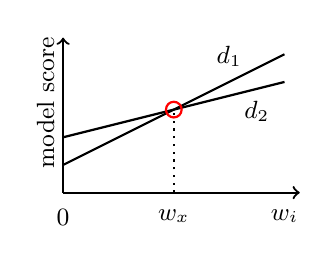
\begin{tikzpicture}
\begin{scope}
\node[anchor=west] (x0) at (0, 0) {};

\draw[->,thick] (x0.center) -- ([xshift=8.2em]x0.east);
\draw[->,thick] (x0.center) -- ([yshift=5.6em]x0.center);

{
\draw[thick] ([yshift=1em]x0.center) -- ([xshift=8em,yshift=5em]x0.center);
\draw[thick] ([yshift=2em]x0.center) -- ([xshift=8em,yshift=4em]x0.center);
\node[anchor=north] (e1) at ([xshift=6em,yshift=6em]x0.south) {\small{$d_1$}};
\node[anchor=north] (e2) at ([xshift=7em,yshift=4em]x0.south) {\small{$d_2$}};
\node[anchor=north,rotate=90] (e2) at ([xshift=-1.3em,yshift=3.6em]x0.south) {\small{model score}};
}

{
\node [anchor=center,draw=red,circle,inner sep=2pt,thick] (x1) at ([xshift=4em,yshift=3em]x0.center) {};
\draw[thick,dotted] ([xshift=4em]x0.center) -- ([xshift=4em,yshift=3em]x0.center);
}
\node[anchor=north] (zero) at ([yshift=0.1em]x0.south) {\small{0}};
\node[anchor=north] (wx) at ([xshift=4em,yshift=0.1em]x0.south) {\small{$w_x$}};
\node[anchor=north] (wi) at ([xshift=8em,yshift=0.1em]x0.south) {\small{$w_i$}};


\end{scope}
\end{tikzpicture}
} &  \subfigure{%%%------------------------------------------------------------------------------------------------------------
%%% 特征权重调优
\begin{tikzpicture}
\begin{scope}
\node[anchor=west] (x0) at (0, 0) {};

\draw[->,thick] (x0.center) -- ([xshift=8.2em]x0.east);
\draw[->,thick] (x0.center) -- ([yshift=5.6em]x0.center);

\node[anchor=north] (zero) at ([yshift=0.1em]x0.south) {\small{0}};
\node[anchor=north] (wx) at ([xshift=4em,yshift=0.1em]x0.south) {\small{$w_x$}};
\node[anchor=north] (wi) at ([xshift=8em,yshift=0.1em]x0.south) {\small{$w_i$}};

{
\draw[thick] ([yshift=2em]x0.center) -- ([xshift=4em,yshift=2em]x0.center);
\draw[thick] ([xshift=4em,yshift=4em]x0.center) -- ([xshift=8em,yshift=4em]x0.center);

\draw[thick,dotted] ([xshift=4em]x0.center) -- ([xshift=4em,yshift=5.5em]x0.center);

\node[anchor=north] (e1) at ([xshift=2em,yshift=3em]x0.north) {\small{$d^*=d_1$}};
\node[anchor=north] (e2) at ([xshift=6.2em,yshift=5em]x0.north) {\small{$d^*=d_2$}};

\node[anchor=north,rotate=90] (e2) at ([xshift=-1.3em,yshift=3.6em]x0.south) {\small{BLEU}};
\draw[decorate,decoration={brace,amplitude=0.4em},red,thick] ([xshift=4em,yshift=0.5em]x0.south) -- ([xshift=8.2em,yshift=0.5em]x0.south);
\node[anchor=north] (wi) at ([xshift=6.1em,yshift=2.1em]x0.south) {\footnotesize{\red{挑选$w_i$}}};
}
\end{scope}
\end{tikzpicture}
} \\
\end{tabular}
\caption{推导得分关于权重的函数以及对应的BLEU值变化}
\label{fig:4-25}
\end{figure}
%-------------------------------------------

\parinterval 这样,最优权重搜索的问题就被转化为找到最优推导BLEU值发生变化的点的问题。理论上,对于$n$-best翻译,交叉点计算最多需要$\frac{n(n-1)}{2}$次。由于$n$一般不会过大,这个时间成本完全是可以接受的。此外,在实现时还有一些技巧,比如,并不需要在每个交叉点处对整个数据集进行BLEU计算,可以只对BLEU产生变化的部分(比如$n$-gram匹配的数量)进行调整,因此搜索的整体效率会进一步得到提高。相比于格搜索,线搜索可以确保在单个特征维度上的最优值,同时保证搜索的效率。

\parinterval 还有一些经验性的技巧用来完善基于线搜索的MERT。例如:

\begin{itemize}
\vspace{0.5em}
\item 随机生成特征权重的起始点;
\vspace{0.5em}
\item 搜索中,给权重加入一些微小的扰动,避免陷入局部最优;
\vspace{0.5em}
\item 随机选择特征优化的顺序;
\vspace{0.5em}
\item 使用先验知识来指导MERT(对权重的取值范围进行约束);
\vspace{0.5em}
\item 使用多轮迭代训练,最终对权重进行平均。
\vspace{0.5em}
\end{itemize}

\parinterval MERT最大的优点在于可以用于目标函数不可微、甚至不连续的情况。对于优化线性模型, MERT是一种很好的选择。但是,也有研究发现,简单使用MERT无法处理特征数量过多的情况。比如,用MERT优化10000个稀疏特征的权重时,优化效果可能会不理想,而且收敛速度慢。这时也可以考虑使用在线学习等技术对大量特征的权重进行调优,比较有代表性的方法包括MIRA\cite{DBLP:conf/emnlp/ChiangMR08}和PRO\cite{Hopkins2011Tuning}。由于篇幅所限,这里不对这些方法做深入讨论,感兴趣的读者可以参考\ref{section-4.5}节的内容,对相关文献进行查阅。

%----------------------------------------------------------------------------------------
%    NEW SUB-SECTION
%----------------------------------------------------------------------------------------

\subsection{栈解码}

\parinterval 解码的目的是根据模型以及输入,找到模型得分最高的推导,即:
\begin{eqnarray}
\hat{d} = \arg\max_{d} \textrm{score}(d,\mathbf{t},\mathbf{s})
\label{eq:4-21}
\end{eqnarray}

\parinterval 然而想要找到得分最高的翻译推导并不是一件简单的事情。对于每一句源语言句子,可能的翻译结果是指数级的。而机器翻译解码也已经被证明是一个NP难问题\cite{knight1999decoding}。简单的暴力搜索显然不现实。因此,在机器翻译中会使用特殊的解码策略来确保搜索的效率。本节将介绍基于栈的自左向右解码方法。它是基于短语的模型中的经典解码方法,非常适于处理语言生成的各种任务。

%----------------------------------------------
\begin{figure}[htp]
\centering
%%%------------------------------------------------------------------------------------------------------------
%%% 什么是解码
\begin{tikzpicture}

\begin{scope}[minimum height = 18pt]

\node[anchor=east] (s0) at (-0.5em, 0) {$\textbf{s}$:};
\node[anchor=west,fill=gray!20] (s1) at (0, 0) {\footnotesize{桌子 上}};
\node[anchor=west,fill=gray!20] (s2) at ([xshift=1em]s1.east) {\footnotesize{有}};
\node[anchor=west,fill=gray!20] (s3) at ([xshift=1em]s2.east) {\footnotesize{一个 苹果}};

\node[anchor=east] (t0) at (-0.5em, -1.5) {$\textbf{t}$:};

\node[anchor=north] (l) at ([xshift=7em,yshift=-0.5em]t0.south) {\footnotesize{(a)\ }};
\end{scope}



\begin{scope}[xshift=15em,minimum height = 18pt]

\node[anchor=east] (s0) at (-0.5em, 0) {$\textbf{s}$:};
\node[anchor=west,fill=gray!20] (s1) at (0, 0) {\footnotesize{桌子 上}};
\node[anchor=west,fill=red!20] (s2) at ([xshift=1em]s1.east) {\footnotesize{有}};
\node[anchor=west,fill=gray!20] (s3) at ([xshift=1em]s2.east) {\footnotesize{一个 苹果}};

\node[anchor=east] (t0) at (-0.5em, -1.5) {$\textbf{t}$:};
{
\node[anchor=west,fill=red!20] (t1) at (0, -1.5) {\footnotesize{There is}};
\path[<->, thick] (s2.south) edge (t1.north);
}

\node[anchor=north] (l) at ([xshift=7em,yshift=-0.5em]t0.south) {\footnotesize{(b)\ }};
\end{scope}



\begin{scope}[yshift=-9.5em,minimum height = 18pt]

\node[anchor=east] (s0) at (-0.5em, 0) {$\textbf{s}$:};
\node[anchor=west,fill=gray!20] (s1) at (0, 0) {\footnotesize{桌子 上}};
\node[anchor=west,fill=gray!20] (s2) at ([xshift=1em]s1.east) {\footnotesize{有}};
\node[anchor=west,fill=red!20] (s3) at ([xshift=1em]s2.east) {\footnotesize{一个 苹果}};

\node[anchor=east] (t0) at (-0.5em, -1.5) {$\textbf{t}$:};
{
\node[anchor=west,fill=gray!20] (t1) at (0, -1.5) {\footnotesize{There is}};
\path[<->, thick] (s2.south) edge (t1.north);
}
{
\node[anchor=west,fill=red!20] (t2) at ([xshift=1em]t1.east) {\footnotesize{an apple}};
\path[<->, thick] (s3.south) edge (t2.north);
}
\node[anchor=north] (l) at ([xshift=7em,yshift=-0.5em]t0.south) {\footnotesize{(c)\ }};
\end{scope}




\begin{scope}[xshift=15em,yshift=-9.5em,minimum height = 18pt]%[scale=0.5]

\node[anchor=east] (s0) at (-0.5em, 0) {$\textbf{s}$:};
\node[anchor=west,fill=red!20] (s1) at (0, 0) {\footnotesize{桌子 上}};
\node[anchor=west,fill=gray!20] (s2) at ([xshift=1em]s1.east) {\footnotesize{有}};
\node[anchor=west,fill=gray!20] (s3) at ([xshift=1em]s2.east) {\footnotesize{一个 苹果}};

\node[anchor=east] (t0) at (-0.5em, -1.5) {$\textbf{t}$:};
{
\node[anchor=west,fill=gray!20] (t1) at (0, -1.5) {\footnotesize{There is}};
\path[<->, thick] (s2.south) edge (t1.north);
}
{
\node[anchor=west,fill=gray!20] (t2) at ([xshift=1em]t1.east) {\footnotesize{an apple}};
\path[<->, thick] (s3.south) edge (t2.north);
}
{
\node[anchor=west,fill=red!20] (t3) at ([xshift=1em]t2.east) {\footnotesize{on the table}};
\path[<->, thick] (s1.south) edge (t3.north);
}
\node[anchor=north] (l) at ([xshift=7em,yshift=-0.5em]t0.south) {\footnotesize{(d)\ }};
\end{scope}
\end{tikzpicture}
\caption{翻译的基本流程}
\label{fig:4-26}
\end{figure}
%-------------------------------------------

\parinterval 首先,看一下翻译一个句子的基本流程。如图\ref{fig:4-26}所示,首先需要得到译文句子的第一个单词。在基于短语的模型中,可以从源语言端找出生成句首译文的短语,之后把译文放到目标语言端,例如,源语言的``有''对应的译文是``There is''。这个过程可以重复执行,直到生成完整句子的译文。但是,有两点需要注意:

\begin{itemize}
\vspace{0.5em}
\item 源语言的每个单词(短语)只能被翻译一次;
\vspace{0.5em}
\item 译文的生成需自左向右连续进行。
\vspace{0.5em}
\end{itemize}

\parinterval 前者对应了一种{\small\bfnew{覆盖度模型}}\index{覆盖度模型}(Coverage Model)\index{Coverage Model};后者定义了解码的方向,这样可以确保$n$-gram语言模型的计算是准确的。这样,就得到了一个简单的基于短语的机器翻译解码框架。每次从源语言句子中找到一个短语,作为译文最右侧的部分,重复执行直到整个译文被生成出来。

%----------------------------------------------------------------------------------------
%    NEW SUBSUB-SECTION
%----------------------------------------------------------------------------------------

\subsubsection{翻译候选匹配}

\parinterval 在解码时,首先要知道每个源语言短语可能的译文都是什么。对于一个源语言短语,每个可能的译文也被称作{\small\bfnew{翻译候选}}\index{翻译候选}(Translation Candidate)\index{Translation Candidate}。实现翻译候选的匹配很简单。只需要遍历输入的源语言句子中所有可能的短语,之后在短语表中找到相应的翻译即可。比如,图\ref{fig:4-27}展示了句子``桌子\ 上\ 有\ 一个\ 苹果''的翻译候选匹配结果。可以看到,不同的短语会对应若干翻译候选。这些翻译候选会保存在所对应的跨度中。比如,``upon the table''是短语``桌子 上 有''的翻译候选,即对应源语言跨度[0,3]。

%----------------------------------------------
\begin{figure}[t]
\centering
%%%------------------------------------------------------------------------------------------------------------
%%% 什么是解码
\begin{center}
\begin{tikzpicture}
\begin{scope}[minimum height = 16pt]

\node[anchor=east] (s0) at (-0.8em, 0) {$\textbf{s}$:};
\node[anchor=west] (s1) at (0, 0) {桌子};
\node[anchor=west] (s2) at ([xshift=2em]s1.east) {上};
\node[anchor=west] (s3) at ([xshift=2.3em]s2.east) {有};
\node[anchor=west] (s4) at ([xshift=2em]s3.east) {一个};
\node[anchor=west] (s5) at ([xshift=1.6em]s4.east) {苹果};

\node [anchor=north,inner sep=2pt,fill=red!20,minimum height=1.5em,minimum width=3em] (t11) at ([yshift=-0.5em]s1.south) {table};
\node [anchor=north,inner sep=2pt,fill=red!20,minimum height=1.5em,minimum width=3em] (t12) at ([yshift=-0.2em]t11.south) {desk};

\node [anchor=north,inner sep=2pt,fill=green!20,minimum height=1.5em,minimum width=3em] (t21) at ([yshift=-0.5em]s2.south) {on};
\node [anchor=north,inner sep=2pt,fill=green!20,minimum height=1.5em,minimum width=3em] (t22) at ([yshift=-0.2em]t21.south) {up};

\node [anchor=north,inner sep=2pt,fill=blue!20,minimum height=1.5em,minimum width=3.4em] (t31) at ([yshift=-0.5em]s3.south) {have};
\node [anchor=north,inner sep=2pt,fill=blue!20,minimum height=1.5em,minimum width=3.4em] (t32) at ([yshift=-0.2em]t31.south) {there is};

\node [anchor=north,inner sep=2pt,fill=orange!20,minimum height=1.5em,minimum width=3em] (t41) at ([yshift=-0.5em]s4.south) {one};
\node [anchor=north,inner sep=2pt,fill=orange!20,minimum height=1.5em,minimum width=3em] (t42) at ([yshift=-0.2em]t41.south) {an};

\node [anchor=north,inner sep=2pt,fill=purple!20,minimum height=1.5em,minimum width=3em] (t51) at ([yshift=-0.5em]s5.south) {apple};
\node [anchor=north,inner sep=2pt,fill=purple!20,minimum height=1.5em,minimum width=3em] (t52) at ([yshift=-0.2em]t51.south) {apples};

\node [anchor=north west,inner sep=2pt,fill=red!20,minimum height=1.5em,minimum width=7.2em] (t13) at ([yshift=-3.7em]t12.south west) {on table};
\node [anchor=north west,inner sep=2pt,fill=red!20,minimum height=1.5em,minimum width=7.2em] (t14) at ([yshift=-0.2em]t13.south west) {on the table};

\node [anchor=north west,inner sep=2pt,fill=orange!20,minimum height=1.5em,minimum width=7.35em] (t43) at ([yshift=-0.2em]t42.south west) {one apple};
\node [anchor=north west,inner sep=2pt,fill=orange!20,minimum height=1.5em,minimum width=7.35em] (t44) at ([yshift=-0.2em]t43.south west) {an apple};

\node [anchor=north west,inner sep=2pt,fill=green!20,minimum height=1.5em,minimum width=7.25em] (t23) at ([yshift=-0.2em]t22.south west) {upon there};

\node [anchor=north west,inner sep=2pt,fill=red!20,minimum height=1.5em,minimum width=11.5em] (t15) at ([yshift=-1.95em]t12.south west) {upon the table};

\node [anchor=north west,inner sep=2pt,fill=blue!20,minimum height=1.5em,minimum width=11.8em] (t33) at ([yshift=-3.7em]t32.south west) {there is an apple};
\node [anchor=north west,inner sep=2pt,fill=blue!20,minimum height=1.5em,minimum width=11.8em] (t34) at ([yshift=-0.2em]t33.south west) {have an apple...};

\end{scope}
\end{tikzpicture}
\end{center}
\caption{一个句子匹配的短语翻译候选}
\label{fig:4-27}
\end{figure}
%-------------------------------------------

%----------------------------------------------------------------------------------------
%    NEW SUBSUB-SECTION
%----------------------------------------------------------------------------------------

\subsubsection{翻译假设扩展}

\parinterval 下一步,需要使用这些翻译候选生成完整的译文。在机器翻译中,一个很重要的概念是{\small\bfnew{翻译假设}}\index{翻译假设}(Translation Hypothesis)\index{Translation Hypothesis}。 它可以被当作是一个局部译文所对应的短语翻译推导。在解码开始时,只有一个空假设,也就是任何译文单词都没有被生成出来。接着,可以挑选翻译选项来扩展当前的翻译假设。

%----------------------------------------------
\begin{figure}[htp]
\centering
%%%------------------------------------------------------------------------------------------------------------
%%% 什么是解码
\begin{center}
\begin{tikzpicture}
\begin{scope}
{
\node [anchor=north,inner sep=2pt,fill=red!20,minimum height=2em,minimum width=3.5em] (h0) at (0,0) {\small{null}};
\node [anchor=north west,inner sep=1.5pt,fill=black] (hl0) at (h0.north west) {\scriptsize{{\color{white} \textbf{0}}}};
\node [anchor=north,rotate=90,inner sep=1pt,minimum width=2em,fill=black] (pt0) at (h0.east) {\footnotesize{{\color{white} \textbf{P=1}}}};
}

{
\node [anchor=west,inner sep=2pt,fill=red!20,minimum height=2em,minimum width=3.5em] (h1) at ([xshift=3em]h0.east) {\small{on}};
\node [anchor=west,inner sep=2pt,fill=red!20,minimum height=2em,minimum width=3.5em] (h2) at ([xshift=3em,yshift=3em]h0.east) {\small{table}};
\node [anchor=west,inner sep=2pt,fill=red!20,minimum height=2em,minimum width=3.5em] (h3) at ([xshift=3em,yshift=-3em]h0.east) {\small{there is}};
\node [anchor=north west,inner sep=1.5pt,fill=black] (hl1) at (h1.north west) {\scriptsize{{\color{white} \textbf{2}}}};
\node [anchor=north west,inner sep=1.5pt,fill=black] (hl2) at (h2.north west) {\scriptsize{{\color{white} \textbf{1}}}};
\node [anchor=north west,inner sep=1.5pt,fill=black] (hl3) at (h3.north west) {\scriptsize{{\color{white} \textbf{3}}}};
\node [anchor=north,rotate=90,inner sep=1pt,minimum width=2em,fill=black] (pt1) at (h1.east) {\footnotesize{{\color{white} \textbf{P=.2}}}};
\node [anchor=north,rotate=90,inner sep=1pt,minimum width=2em,fill=black] (pt2) at (h2.east) {\footnotesize{{\color{white} \textbf{P=.3}}}};
\node [anchor=north,rotate=90,inner sep=1pt,minimum width=2em,fill=black] (pt3) at (h3.east) {\footnotesize{{\color{white} \textbf{P=.5}}}};

\draw [->,very thick,ublue] ([xshift=0.1em]pt0.south) -- ([xshift=-0.1em]h1.west);
\draw [->,very thick,ublue] ([xshift=0.1em]pt0.south) -- ([xshift=-0.1em]h2.west);
\draw [->,very thick,ublue] ([xshift=0.1em]pt0.south) -- ([xshift=-0.1em]h3.west);
}

{
\node [anchor=west,inner sep=2pt,fill=red!20,minimum height=2em,minimum width=3.5em] (h4) at ([xshift=3em,yshift=-1.8em]h3.east) {\small{one}};
\node [anchor=west,inner sep=2pt,fill=red!20,minimum height=2em,minimum width=3.5em] (h5) at ([xshift=3em,yshift=1.2em]h3.east) {\small{an apple}};
\node [anchor=west,inner sep=2pt,fill=red!20,minimum height=2em,minimum width=3.5em] (h6) at ([xshift=3em,yshift=1.2em]h1.east) {\small{table}};
\node [anchor=west,inner sep=2pt,fill=red!20,minimum height=2em,minimum width=4em] (h7) at ([xshift=3em,yshift=1.2em]h5.east) {\small{on the table}};
\node [anchor=west,inner sep=2pt,fill=red!20,minimum height=2em,minimum width=4.6em] (h8) at ([xshift=3em,yshift=-2em]h5.east) {\small{\ \;apple}};

\node [anchor=north west,inner sep=1.5pt,fill=black] (hl4) at (h4.north west) {\scriptsize{{\color{white} \textbf{4}}}};
\node [anchor=north west,inner sep=1.5pt,fill=black] (hl5) at (h5.north west) {\scriptsize{{\color{white} \textbf{4-5}}}};
\node [anchor=north west,inner sep=1.5pt,fill=black] (hl6) at (h6.north west) {\scriptsize{{\color{white} \textbf{1}}}};
\node [anchor=north west,inner sep=1.5pt,fill=black] (hl7) at (h7.north west) {\scriptsize{{\color{white} \textbf{1-2}}}};
\node [anchor=north west,inner sep=1.5pt,fill=black] (hl8) at (h8.north west) {\scriptsize{{\color{white} \textbf{5}}}};

\node [anchor=north,rotate=90,inner sep=1pt,minimum width=2em,fill=black] (pt4) at (h4.east) {\footnotesize{{\color{white} \textbf{P=.1}}}};
\node [anchor=north,rotate=90,inner sep=1pt,minimum width=2em,fill=black] (pt5) at (h5.east) {\footnotesize{{\color{white} \textbf{P=.4}}}};
\node [anchor=north,rotate=90,inner sep=1pt,minimum width=2em,fill=black] (pt6) at (h6.east) {\footnotesize{{\color{white} \textbf{P=.3}}}};
\node [anchor=north,rotate=90,inner sep=1pt,minimum width=2em,fill=black] (pt7) at (h7.east) {\footnotesize{{\color{white} \textbf{P=.4}}}};
\node [anchor=north,rotate=90,inner sep=1pt,minimum width=2em,fill=black] (pt8) at (h8.east) {\footnotesize{{\color{white} \textbf{P=.2}}}};

\draw [->,very thick,ublue] ([xshift=0.1em]pt1.south) -- ([xshift=1em,yshift=0.7em]pt1.south);

\draw [->,very thick,ublue] ([xshift=0.1em]pt2.south) -- ([xshift=1em,yshift=-0.7em]pt2.south);
\draw [->,very thick,ublue] ([xshift=0.1em]pt2.south) -- ([xshift=1em,yshift=0.7em]pt2.south);

\draw [->,very thick,ublue] ([xshift=0.1em]pt6.south) -- ([xshift=1em,yshift=-0.7em]pt6.south);
\draw [->,very thick,ublue] ([xshift=0.1em]pt6.south) -- ([xshift=1em,yshift=0.7em]pt6.south);

\draw [->,very thick,ublue] ([xshift=0.1em]pt3.south) -- ([xshift=-0.1em]h4.west);
\draw [->,very thick,ublue] ([xshift=0.1em]pt3.south) -- ([xshift=-0.1em]h5.west);
\draw [->,very thick,ublue] ([xshift=0.1em]pt3.south) -- ([xshift=-0.1em]h6.west);

\draw [->,very thick,ublue] ([xshift=0.1em]pt5.south) -- ([xshift=-0.1em]h7.west);
\draw [->,very thick,ublue] ([xshift=0.1em]pt5.south) -- ([xshift=1em,yshift=-0.7em]pt5.south);

\draw [->,very thick,ublue] ([xshift=0.1em]pt4.south) -- ([xshift=-0.1em]h8.west);
\draw [->,very thick,ublue] ([xshift=0.1em]pt4.south) -- ([xshift=1em,yshift=-0.7em]pt4.south);
}

{
\draw [->,ultra thick,red,line width=2pt,opacity=0.7] ([xshift=-0.5em]h0.west) -- ([xshift=0.7em]h0.east) -- ([xshift=-0.2em]h3.west) -- ([xshift=0.8em]h3.east) -- ([xshift=-0.2em]h5.west) -- ([xshift=0.8em]h5.east) -- ([xshift=-0.2em]h7.west) -- ([xshift=1.5em]h7.east);
\node [anchor=north west] (wtranslabel) at ([yshift=-3em]h0.south west) {\small{翻译路径:}};
\draw [->,ultra thick,red,line width=1.5pt,opacity=0.7] (wtranslabel.east) -- ([xshift=1.5em]wtranslabel.east);
}
\end{scope}
\end{tikzpicture}
\end{center}
\caption{翻译假设扩展}
\label{fig:4-28}
\end{figure}
%-------------------------------------------

\parinterval 图\ref{fig:4-28}展示了翻译假设扩展的过程。在翻译假设扩展时,需要保证新加入的翻译候选放置在旧翻译假设译文的右侧,也就是要确保翻译自左向右的连续性。而且,同一个翻译假设可以使用不同的翻译候选进行扩展。例如,扩展第一个翻译假设时,可以选择``桌子''的翻译候选``table'';也可以选择``有''的翻译候选``There is''。扩展完之后需要记录输入句子中已翻译的短语,同时计算当前所有翻译假设的模型得分。这个过程相当于生成了一个图的结构,每个节点代表了一个翻译假设。当翻译假设覆盖了输入句子所有的短语,不能被继续扩展时,就生成了一个完整的翻译假设(译文)。最后需要找到得分最高的完整翻译假设,它对应了搜索图中的最优路径。

%----------------------------------------------------------------------------------------
%    NEW SUBSUB-SECTION
%----------------------------------------------------------------------------------------

\subsubsection{剪枝}

\parinterval 假设扩展建立了解码算法的基本框架。但是,当句子变长时,这种方法还是面临着搜索空间爆炸的问题。对于这个问题,常用的解决办法是{\small\bfnew{剪枝}}\index{剪枝}(Pruning)\index{Pruning},也就是在搜索图中排除掉一些节点。比如,可以使用{\small\bfnew{束剪枝}}\index{束剪枝}(Beam Pruning)\index{Beam Pruning},确保每次翻译扩展时,最多生成$k$个新的翻译假设。这里$k$可以被看做是束的宽度。通过控制$k$的大小,可以在解码精度和速度之间进行平衡。这种基于束宽度进行剪枝的方法也被称作{\small\bfnew{直方图剪枝}}\index{直方图剪枝}(Histogram Pruning)\index{Histogram Pruning}。另一种思路是,每次扩展时只保留与最优翻译假设得分相差在$\delta$之内的翻译假设。$\delta$可以被看作是一种与最优翻译假设之间距离的阈值,超过这个阈值就被剪枝。这种方法也被称作{\small\bfnew{阈值剪枝}}\index{阈值剪枝}(Threshold Pruning)\index{Threshold Pruning}。

\parinterval 不过,即使引入束剪枝,解码过程中仍然会有很多冗余的翻译假设。有两种方法可以进一步加速解码:

\begin{itemize}
\vspace{0.5em}
\item 对相同译文的翻译假设进行重新组合;
\vspace{0.5em}
\item 对低质量的翻译假设进行裁剪。
\vspace{0.5em}
\end{itemize}

\parinterval 对翻译假设进行重新组合又被称作{\small\bfnew{假设重组}}\index{假设重组}(Hypothesis Recombination)\index{Hypothesis Recombination}。其核心思想是,把代表同一个译文的不同翻译假设融合为一个翻译假设。如图29所示,对于给定的输入短语``一个\ \ 苹果'',系统可能将两个单词``一个''、``苹果''分别翻译成``an''和``apple'',也可能将这两个单词作为一个短语直接翻译成``an apple''。虽然这两个翻译假设得到的译文相同,并且覆盖了相同的源语言短语,但是却是两个不同的翻译假设,模型给它们的打分也是不一样的。这时,可以舍弃两个翻译假设中分数较低的那个,因为分数较低的翻译假设永远不可能成为最优路径的一部分。这也就相当于把两个翻译假设重组为一个假设。

%----------------------------------------------
\begin{figure}[htp]
\centering
%%%------------------------------------------------------------------------------------------------------------
%%% 假设重组
\begin{tikzpicture}
\begin{scope}
{
\node [anchor=north,inner sep=2pt,fill=red!20,minimum height=2em,minimum width=3em] (h0) at (0,0) {\small{null}};
\node [anchor=north west,inner sep=1.0pt,fill=black] (hl0) at (h0.north west) {\scriptsize{{\color{white} \textbf{0}}}};
\node [anchor=north,rotate=90,inner sep=1pt,minimum width=2em,fill=black] (pt0) at (h0.east) {\footnotesize{{\color{white} \textbf{P=1}}}};

\node [anchor=west,inner sep=2pt,fill=red!20,minimum height=2em,minimum width=3em] (h2) at ([xshift=2.2em,yshift=3.5em]h0.east) {\small{an}};
\node [anchor=west,inner sep=2pt,fill=red!20,minimum height=2em,minimum width=3em] (h3) at ([xshift=2.2em]h2.east) {\small{apple}};

\node [anchor=north west,inner sep=1.0pt,fill=black] (hl2) at (h2.north west) {\scriptsize{{\color{white} \textbf{1}}}};
\node [anchor=north west,inner sep=1.0pt,fill=black] (hl3) at (h3.north west) {\scriptsize{{\color{white} \textbf{2}}}};

\node [anchor=north,rotate=90,inner sep=1pt,minimum width=2em,fill=black] (pt2) at (h2.east) {\footnotesize{{\color{white} \textbf{P=.3}}}};
\node [anchor=north,rotate=90,inner sep=1pt,minimum width=2em,fill=black] (pt3) at (h3.east) {\footnotesize{{\color{white} \textbf{P=.5}}}};

\draw [->,very thick,ublue] ([xshift=0.1em]pt0.south) -- ([xshift=-0.1em]h2.west);
\draw [->,very thick,ublue] ([xshift=0.1em]pt2.south) -- ([xshift=-0.1em]h3.west);

{
\node [anchor=west,inner sep=2pt,fill=red!20,minimum height=2em,minimum width=3em] (h1) at ([xshift=7em]h0.east) {\small{an apple}};
\node [anchor=north west,inner sep=1.0pt,fill=black] (hl1) at (h1.north west) {\scriptsize{{\color{white} \textbf{1-2}}}};
\node [anchor=north,rotate=90,inner sep=1pt,minimum width=2em,fill=black] (pt1) at (h1.east) {\footnotesize{{\color{white} \textbf{P=.5}}}};
\draw [->,very thick,ublue] ([xshift=0.1em]pt0.south) -- ([xshift=-0.1em]h1.west);
}
}
{
\node [anchor=north west,inner sep=2pt,fill=red!20,minimum height=2em,minimum width=3em] (h4) at ([yshift=-7em]h0.south west) {\small{null}};
\node [anchor=west,inner sep=2pt,fill=red!20,minimum height=2em,minimum width=3em] (h5) at ([xshift=2.2em]h4.east) {\small{he}};
\node [anchor=west,inner sep=2pt,fill=red!20,minimum height=2em,minimum width=3em] (h6) at ([xshift=2.2em,yshift=3.5em]h4.east) {\small{it}};
\node [anchor=west,inner sep=2pt,fill=red!20,minimum height=2em,minimum width=3em] (h8) at ([xshift=2.2em]h6.east) {\small{is not}};

\node [anchor=north west,inner sep=1.0pt,fill=black] (hl4) at (h4.north west) {\scriptsize{{\color{white} \textbf{0}}}};
\node [anchor=north west,inner sep=1.0pt,fill=black] (hl5) at (h5.north west) {\scriptsize{{\color{white} \textbf{1}}}};
\node [anchor=north west,inner sep=1.0pt,fill=black] (hl5) at (h6.north west) {\scriptsize{{\color{white} \textbf{1}}}};

\node [anchor=north west,inner sep=1.0pt,fill=black] (hl5) at (h8.north west) {\scriptsize{{\color{white} \textbf{2}}}};
\node [anchor=north,rotate=90,inner sep=1pt,minimum width=2em,fill=black] (pt4) at (h4.east) {\footnotesize{{\color{white} \textbf{P=1}}}};
\node [anchor=north,rotate=90,inner sep=1pt,minimum width=2em,fill=black] (pt5) at (h5.east) {\footnotesize{{\color{white} \textbf{P=.3}}}};
\node [anchor=north,rotate=90,inner sep=1pt,minimum width=2em,fill=black] (pt6) at (h6.east) {\footnotesize{{\color{white} \textbf{P=.4}}}};
\node [anchor=north,rotate=90,inner sep=1pt,minimum width=2em,fill=black] (pt8) at (h8.east) {\footnotesize{{\color{white} \textbf{P=.2}}}};

\draw [->,very thick,ublue] ([xshift=0.1em]pt4.south) -- ([xshift=-0.1em]h5.west);
\draw [->,very thick,ublue] ([xshift=0.1em]pt4.south) -- ([xshift=-0.1em]h6.west);
\draw [->,very thick,ublue] ([xshift=0.1em]pt6.south) -- ([xshift=-0.1em]h8.west);

{
\node [anchor=west,inner sep=2pt,fill=red!20,minimum height=2em,minimum width=3em] (h7) at ([xshift=2.2em]h5.east) {\small{is not}};
\node [anchor=north,rotate=90,inner sep=1pt,minimum width=2em,fill=black] (pt7) at (h7.east) {\footnotesize{{\color{white} \textbf{P=.2}}}};
\node [anchor=north west,inner sep=1.0pt,fill=black] (hl5) at (h7.north west) {\scriptsize{{\color{white} \textbf{2}}}};
\draw [->,very thick,ublue] ([xshift=0.1em]pt5.south) -- ([xshift=-0.1em]h7.west);
}
}

\node[anchor=north] (l1) at ([xshift=6em,yshift=-1em]h0.south) {\scriptsize{(a)\ 原假设(译文相同时)}};
\node[anchor=north] (l2) at ([xshift=6em,yshift=-1em]h4.south) {\scriptsize{(c)\ 原假设(译文不同时)}};
%\node [anchor=west,inner sep=2pt,fill=red!20,minimum height=2em,minimum width=3em,opacity=0.7] (h1) at ([xshift=-1em,yshift=2em]h2.north) {原假设};

\end{scope}





\begin{scope}[xshift = 16em, yshift = 0em]
{
\node [anchor=north,inner sep=2pt,fill=red!20,minimum height=2em,minimum width=3em] (h0) at (0,0) {\small{null}};
\node [anchor=north west,inner sep=1.0pt,fill=black] (hl0) at (h0.north west) {\scriptsize{{\color{white} \textbf{0}}}};
\node [anchor=north,rotate=90,inner sep=1pt,minimum width=2em,fill=black] (pt0) at (h0.east) {\footnotesize{{\color{white} \textbf{P=1}}}};

\node [anchor=west,inner sep=2pt,fill=red!20,minimum height=2em,minimum width=3em] (h2) at ([xshift=2.2em,yshift=3.5em]h0.east) {\small{an}};
\node [anchor=west,inner sep=2pt,fill=red!20,minimum height=2em,minimum width=3em] (h3) at ([xshift=2.2em]h2.east) {\small{apple}};

\node [anchor=north west,inner sep=1.0pt,fill=black] (hl2) at (h2.north west) {\scriptsize{{\color{white} \textbf{1}}}};
\node [anchor=north west,inner sep=1.0pt,fill=black] (hl3) at (h3.north west) {\scriptsize{{\color{white} \textbf{2}}}};

\node [anchor=north,rotate=90,inner sep=1pt,minimum width=2em,fill=black] (pt2) at (h2.east) {\footnotesize{{\color{white} \textbf{P=.3}}}};
\node [anchor=north,rotate=90,inner sep=1pt,minimum width=2em,fill=black] (pt3) at (h3.east) {\footnotesize{{\color{white} \textbf{P=.5}}}};

\draw [->,very thick,ublue] ([xshift=0.1em]pt0.south) -- ([xshift=-0.1em]h2.west);
\draw [->,very thick,ublue] ([xshift=0.1em]pt2.south) -- ([xshift=-0.1em]h3.west);

{
\draw [->,ultra thick,red,line width=2pt,opacity=0.7] ([xshift=0.1em]pt0.south) -- ([xshift=-1em,yshift=-0.1em]h3.south);
}
}
{
\node [anchor=north west,inner sep=2pt,fill=red!20,minimum height=2em,minimum width=3em] (h4) at ([yshift=-7em]h0.south west) {\small{null}};
\node [anchor=west,inner sep=2pt,fill=red!20,minimum height=2em,minimum width=3em] (h5) at ([xshift=2.2em]h4.east) {\small{he}};
\node [anchor=west,inner sep=2pt,fill=red!20,minimum height=2em,minimum width=3em] (h6) at ([xshift=2.2em,yshift=3.5em]h4.east) {\small{it}};
\node [anchor=west,inner sep=2pt,fill=red!20,minimum height=2em,minimum width=3em] (h8) at ([xshift=2.2em]h6.east) {\small{is not}};

\node [anchor=north west,inner sep=1.0pt,fill=black] (hl4) at (h4.north west) {\scriptsize{{\color{white} \textbf{0}}}};
\node [anchor=north west,inner sep=1.0pt,fill=black] (hl5) at (h5.north west) {\scriptsize{{\color{white} \textbf{1}}}};
\node [anchor=north west,inner sep=1.0pt,fill=black] (hl5) at (h6.north west) {\scriptsize{{\color{white} \textbf{1}}}};

\node [anchor=north west,inner sep=1.0pt,fill=black] (hl5) at (h8.north west) {\scriptsize{{\color{white} \textbf{2}}}};
\node [anchor=north,rotate=90,inner sep=1pt,minimum width=2em,fill=black] (pt4) at (h4.east) {\footnotesize{{\color{white} \textbf{P=1}}}};
\node [anchor=north,rotate=90,inner sep=1pt,minimum width=2em,fill=black] (pt5) at (h5.east) {\footnotesize{{\color{white} \textbf{P=.3}}}};
\node [anchor=north,rotate=90,inner sep=1pt,minimum width=2em,fill=black] (pt6) at (h6.east) {\footnotesize{{\color{white} \textbf{P=.4}}}};
\node [anchor=north,rotate=90,inner sep=1pt,minimum width=2em,fill=black] (pt8) at (h8.east) {\footnotesize{{\color{white} \textbf{P=.2}}}};

\draw [->,very thick,ublue] ([xshift=0.1em]pt4.south) -- ([xshift=-0.1em]h5.west);
\draw [->,very thick,ublue] ([xshift=0.1em]pt4.south) -- ([xshift=-0.1em]h6.west);
\draw [->,very thick,ublue] ([xshift=0.1em]pt6.south) -- ([xshift=-0.1em]h8.west);

{
\draw [->,ultra thick,red,line width=2pt,opacity=0.7] ([xshift=0.1em]pt5.south) -- ([xshift=-1em,yshift=-0.1em]h8.south);
}
}



{
{
\node [anchor=west,inner sep=2pt,fill=red!20,minimum height=2em,minimum width=3em,opacity=0.3] (h1) at ([xshift=7em]h0.east) {\small{an apple}};
\node [anchor=north west,inner sep=1.0pt,fill=black,opacity=0.3] (hl1) at (h1.north west) {\scriptsize{{\color{white} \textbf{1-2}}}};
\node [anchor=north,rotate=90,inner sep=1pt,minimum width=2em,fill=black,opacity=0.3] (pt1) at (h1.east) {\footnotesize{{\color{white} \textbf{P=.5}}}};
}
{
\node [anchor=west,inner sep=2pt,fill=red!20,minimum height=2em,minimum width=3em,opacity=0.3] (h7) at ([xshift=2.2em]h5.east) {\small{is not}};
\node [anchor=north,rotate=90,inner sep=1pt,minimum width=2em,fill=black,opacity=0.3] (pt7) at (h7.east) {\footnotesize{{\color{white} \textbf{P=.2}}}};
\node [anchor=north west,inner sep=1.0pt,fill=black,opacity=0.3] (hl5) at (h7.north west) {\scriptsize{{\color{white} \textbf{2}}}};
}
}

\node [anchor=west] (l1) at ([xshift=1em, yshift=0.5em]h1.east) {\footnotesize{舍弃概率}};
\node [anchor=west] (l11) at ([xshift=0em, yshift=-1em]l1.west) {\footnotesize{较低假设}};
\node [anchor=west] (l2) at ([xshift=1em, yshift=0.5em]h7.east) {\footnotesize{舍弃概率}};
\node [anchor=west] (l21) at ([xshift=0em, yshift=-1em]l2.west) {\footnotesize{较低假设}};

%\node [anchor=west,inner sep=2pt,fill=red!20,minimum height=2em,minimum width=3em,opacity=0.7] (h1) at ([xshift=-1em,yshift=2em]h2.north) {重组假设};
\node[anchor=north] (l1) at ([xshift=6em,yshift=-1em]h0.south) {\scriptsize{(c)\ 重组假设(译文相同时)}};
\node[anchor=north] (l2) at ([xshift=6em,yshift=-1em]h4.south) {\scriptsize{(d)\ 重组假设(译文不同时)}};

\end{scope}




\end{tikzpicture}
\caption{假设重组示例}
\label{fig:4-29}
\end{figure}
%-------------------------------------------

\parinterval 即使翻译假设对应的译文不同也可以进行假设重组。图\ref{fig:4-29}的下半部分给出了一个这样的实例。在两个翻译假设中,第一个单词分别被翻译成了``it''和``he'',紧接着它们后面的部分都被翻译成了``is not''。这两个翻译假设是非常相似的,因为它们译文的最后两个单词是相同的,而且翻译假设都覆盖了相同的源语言部分。这时,也可以对这两个翻译假设进行假设重组:如果得分较低的翻译假设和得分较高的翻译假设都使用相同的翻译候选进行扩展,且两个翻译假设都覆盖相同的源语言单词,分数低的翻译假设可以被剪枝掉。此外,还有两点需要注意:

\begin{itemize}
\vspace{0.5em}
\item $n$-gram语言模型将前$n-1$单词作为历史信息,所以当两个假设最后$n-1$个单词不相同时,不能进行假设重组,因为后续的扩展可能会得到不同的语言模型得分,并影响最终的模型得分;
\vspace{0.5em}
\item 调序模型通常是用来判断当前输入的短语与前一个输入短语之间的调序代价。因此当两个翻译假设对应短语在源语言中的顺序不同时,也不能被重新组合。
\vspace{0.5em}
\end{itemize}

\parinterval 然而在实际处理中,并不需要``删掉''分数低的翻译假设,而是将它们与分数高的翻译假设连在了一起。对于搜索最优翻译,这些连接可能并没有什么作用,但是如果需要分数最高的前两个或前三个翻译,就可能需要用到这些连接。

\parinterval 翻译假设的重组有效地减少了解码过程中相同或者相似翻译假设带来的冗余。因此这些方法在机器翻译中被广泛使用。包括本章后面将要介绍的基于句法的翻译模型解码中,也可以使用假设重组进行系统加速。

%----------------------------------------------------------------------------------------
%    NEW SUBSUB-SECTION
%----------------------------------------------------------------------------------------

\subsubsection{解码中的栈结构}

\parinterval 当质量较差的翻译假设在扩展早期出现时,这些翻译假设需要被剪枝掉,这样可以忽略所有从它扩展出来的翻译假设,进而有效地减小搜索空间。但是这样做也存在着一定的问题,首先,删除的翻译假设可能会在后续的扩展过程中被重新搜索出来。其次,过早地删除某些翻译假设可能会导致无法搜索到最优的翻译假设。所以最好的情况是尽早删除质量差的翻译假设,同时又不会对整个搜索结果产生过大影响。但是这个``质量''从哪个方面来衡量,也是一个需要思考的问题。理想的情况就是从早期的翻译假设中,挑选一些可比的翻译假设进行筛选。

\parinterval 目前比较通用的做法是将翻译假设进行整理,放进一种栈结构中。这里所说的``栈''是为了描述方便的一种说法。它实际上就是保存多个翻译假设的一种数据结构\footnote[4]{虽然被称作栈,实际上使用一个堆进行实现。这样可以根据模型得分对翻译假设进行排序。}。当放入栈的翻译假设超过一定阈值时(比如200),可以删除掉模型得分低的翻译假设。一般,会使用多个栈来保存翻译假设,每个栈代表覆盖源语言单词数量相同的翻译假设。

\parinterval 比如,第一个堆栈包含了覆盖一个源语言单词的翻译假设,第二个堆栈包含了覆盖两个源语言单词的翻译假设,以此类推。利用覆盖源语言单词数进行栈的划分的原因在于:翻译相同数量的单词所对应的翻译假设一般是``可比的'',因此在同一个栈里对它们进行剪枝带来的风险较小。

\parinterval 在基于栈的解码中,每次都会从所有的栈中弹出一个翻译假设,并选择一个或者若干个翻译假设进行扩展,之后把新得到的翻译假设重新压入解码栈中。这个过程不断执行,并可以配合束剪枝、假设重组等技术。最后在覆盖所有源语言单词的栈中得到整个句子的译文。图\ref{fig:4-30}展示了一个简单的栈解码过程。第一个栈(0号栈)用来存放空翻译假设。之后通过假设扩展,不断将翻译假设填入对应的栈中。

%----------------------------------------------
\begin{figure}[htp]
\centering
%%%------------------------------------------------------------------------------------------------------------
%%% 栈解码
\begin{center}
\begin{tikzpicture}
\begin{scope}
{
\node [anchor=north,inner sep=2pt,fill=red!20,minimum height=2em,minimum width=3em] (h0) at (0,0) {\scriptsize{null}};
\node [anchor=north west,inner sep=1.5pt,fill=black] (hl0) at (h0.north west) {\scriptsize{{\color{white} \textbf{0}}}};
\node [anchor=north,rotate=90,inner sep=1pt,minimum width=2em,fill=black] (pt0) at (h0.east) {\scriptsize{{\color{white} \textbf{P=1}}}};
}
{
\node [anchor=west,inner sep=2pt,fill=red!20,minimum height=2em,minimum width=3em] (h13) at ([xshift=2.1em,yshift=6em]h0.east) {\scriptsize{there is}};
\node [anchor=west,inner sep=2pt,minimum height=2em,minimum width=3em] (h12) at ([xshift=2.1em,yshift=3.5em]h0.east) {\small{\textbf{...}}};
\node [anchor=west,inner sep=2pt,fill=red!20,minimum height=2em,minimum width=3em] (h1) at ([xshift=2.1em]h0.east) {\scriptsize{tabel}};

\node [anchor=north west,inner sep=1.0pt,fill=black] (hl1) at (h1.north west) {\scriptsize{{\color{white} \textbf{1}}}};
\node [anchor=north west,inner sep=1.0pt,fill=black] (hl3) at (h13.north west) {\scriptsize{{\color{white} \textbf{3}}}};


\node [anchor=north,rotate=90,inner sep=1pt,minimum width=2em,fill=black] (pt1) at (h1.east) {\scriptsize{{\color{white} \textbf{P=.2}}}};
\node [anchor=north,rotate=90,inner sep=1pt,minimum width=2em,fill=black] (pt3) at (h13.east) {\scriptsize{{\color{white} \textbf{P=.5}}}};

\node [anchor=west,inner sep=2pt,fill=red!20,minimum height=2em,minimum width=3em] (h2) at ([xshift=2.1em]h1.east) {\scriptsize{have}};
\node [anchor=west,inner sep=2pt,minimum height=2em,minimum width=3em] (h22) at ([xshift=2.1em]h12.east) {\small{\textbf{...}}};
\node [anchor=west,inner sep=2pt,fill=red!20,minimum height=2em,minimum width=3em] (h23) at ([xshift=2.1em]h13.east) {\scriptsize{an}};
\node [anchor=west,inner sep=2pt,fill=red!20,minimum height=2em,minimum width=3em] (h3) at ([xshift=2.1em]h2.east) {\scriptsize{there is}};
\node [anchor=west,inner sep=2pt,minimum height=2em,minimum width=3em] (h32) at ([xshift=2.1em]h22.east) {\small{\textbf{...}}};
\node [anchor=west,inner sep=2pt,fill=red!20,minimum height=2em,minimum width=3em] (h33) at ([xshift=2.1em]h23.east) {\scriptsize{an apple}};

\node [anchor=north west,inner sep=1.0pt,fill=black] (hl2) at (h2.north west) {\scriptsize{{\color{white} \textbf{3}}}};
\node [anchor=north west,inner sep=1.0pt,fill=black] (hl23) at (h23.north west) {\scriptsize{{\color{white} \textbf{4}}}};
\node [anchor=north west,inner sep=1.0pt,fill=black] (hl3) at (h3.north west) {\scriptsize{{\color{white} \textbf{2}}}};
\node [anchor=north west,inner sep=1.0pt,fill=black] (hl33) at (h33.north west) {\scriptsize{{\color{white} \textbf{4-5}}}};

\node [anchor=north,rotate=90,inner sep=1pt,minimum width=2em,fill=black] (pt2) at (h2.east) {\scriptsize{{\color{white} \textbf{P=.5}}}};
\node [anchor=north,rotate=90,inner sep=1pt,minimum width=2em,fill=black] (pt23) at (h23.east) {\scriptsize{{\color{white} \textbf{P=.5}}}};
\node [anchor=north,rotate=90,inner sep=1pt,minimum width=2em,fill=black] (pt3) at (h3.east) {\scriptsize{{\color{white} \textbf{P=.5}}}};
\node [anchor=north,rotate=90,inner sep=1pt,minimum width=2em,fill=black] (pt33) at (h33.east) {\scriptsize{{\color{white} \textbf{P=.5}}}};
}
\node [anchor=north] (l0) at ([xshift=0.2em,yshift=-0.7em]h0.south) {\small{\textbf{未译词}}};
\node [anchor=north] (l1) at ([xshift=0.3em,yshift=-0.7em]h1.south) {\small{\textbf{已译1词}}};
\node [anchor=north] (l2) at ([xshift=0.3em,yshift=-0.7em]h2.south) {\small{\textbf{已译2词}}};
\node [anchor=north] (l3) at ([xshift=0.3em,yshift=-0.7em]h3.south) {\small{\textbf{已译3词}}};

\begin{pgfonlayer}{background}
\node [rectangle,inner sep=0.3em,fill=blue!10] [fit = (h0) (pt0)] (box0) {};
\node [rectangle,inner sep=0.3em,fill=blue!10] [fit = (h1) (pt1) (h13)] (box1) {};
\node [rectangle,inner sep=0.3em,fill=blue!10] [fit = (h2) (pt2) (h23)] (box2) {};
\node [rectangle,inner sep=0.3em,fill=blue!10] [fit = (h3) (pt3) (h33)] (box3) {};
\end{pgfonlayer}

{
\draw [->,thick,red] (h13.north).. controls +(60:0.5) and +(120:0.5) .. (h23.north);
\draw [->,thick,red] (h13.north).. controls +(58:0.8) and +(122:0.8) .. (h33.north);
\draw [->,thick,red] (h1.north).. controls +(60:0.5) and +(120:0.5) .. (h2.north);
\draw [->,thick,red] (h2.north).. controls +(60:0.5) and +(120:0.5) .. (h3.north);
}
\node [anchor=south east] (wtranslabel) at ([xshift=-1.5em,yshift=-2.2em]h0.south west) {\small{\textbf{:假设堆栈}}};
\node [anchor=east,inner sep=2pt,fill=blue!10,minimum height=1em,minimum width=2em] (stacklabel) at ([xshift=-0.1em]wtranslabel.west) {};
{
\node [anchor=east] (line1) at ([xshift=-1.0em,yshift=0.4em]h0.west) {\small{0号栈包含空假设}};
}
{
\node [anchor=east] (line2) at ([xshift=-2.3em,yshift=0.5em]h13.west) {\small{通过假设扩展产生新的假设}};
\node [anchor=north west] (line3) at ([yshift=0.1em]line2.south west) {\small{并不断的被存入假设堆栈中}};
}
\begin{pgfonlayer}{background}
{
\node [rectangle,inner sep=0.1em,fill=ugreen!10] [fit = (line1)] (box1) {};
}
{
\node [rectangle,inner sep=0.1em,fill=red!10] [fit = (line2) (line3)] (box2) {};
}
\end{pgfonlayer}

\end{scope}
\end{tikzpicture}
\end{center}
\caption{栈解码示例}
\label{fig:4-30}
\end{figure}
%-------------------------------------------

%----------------------------------------------------------------------------------------
%    NEW SECTION
%----------------------------------------------------------------------------------------

\sectionnewpage
\section{基于层次短语的模型}\label{section-4.3}

\parinterval 在机器翻译中,如果翻译需要局部上下文的信息,把短语作为翻译单元是一种理想的方案。但是,单词之间的关系并不总是``局部''的,很多时候需要距离更远一些的搭配。比较典型的例子是含有从句的情况。比如:
\begin{eqnarray}
\qquad \textrm{{\small\bfnew{我}}\ \ 在\ \ 今天\ \ 早上\ \ 没有\ \ 吃\ \ 早\ \ 饭\ \ 的\ \ 情况\ \ 下\ \ 还是\ \ 正常\ \ {\small\bfnew{去}}\ \ {\small\bfnew{上班}}\ \ 了。} \nonumber
\end{eqnarray}

\parinterval 这句话的主语``我''和谓语``去\ 上班''构成了主谓搭配,而二者之间的部分是状语。显然,用短语去捕捉这个搭配需要覆盖很长的词串,也就是整个``我 $...$ 去 上班''的部分。如果把这样的短语考虑到建模中,会面临非常严重的数据稀疏问题,因为无法保证这么长的词串在训练数据中能够出现。

%----------------------------------------------
\begin{table}[htp]{
\begin{center}
\caption{不同短语在训练数据中出现的频次}
\label{tab:4-1}
\begin{tabular}{p{12em} | r}
短语(中文) & 训练数据中出现的频次 \\
\hline

包含 & 3341\\
包含\ 多个 & 213\\
包含\ 多个\ 词 & 12\\
包含\ 多个\ 词\ 的 & 8\\
包含\ 多个\ 词\ 的\ 短语 & 0\\
包含\ 多个\ 词\ 的\ 短语\ 太多 & 0\\
\end{tabular}
\end{center}
}\end{table}
%-------------------------------------------

\parinterval 实际上,随着短语长度变长,短语在数据中会变得越来越低频,相关的统计特征也会越来越不可靠。表\ref{tab:4-1}就展示了不同长度的短语在训练数据中出现的频次。可以看到,长度超过3的短语已经非常低频了,更长的短语甚至在训练数据中一次也没有出现过。

\parinterval 显然,利用过长的短语来处理长距离的依赖并不是一种十分有效的方法。过于低频的长短语无法提供可靠的信息,而且使用长短语会导致模型体积急剧增加。

\parinterval 再来看一个翻译实例\cite{Chiang2012Hope},图\ref{fig:4-31}是一个基于短语的机器翻译系统的翻译结果。这个例子中的调序有一些复杂,比如,``少数\ 国家\ 之一''和``与\ 北韩\ 有\ 邦交''的英文翻译都需要进行调序,分别是``one of the few countries''和``have diplomatic relations with North Korea''。基于短语的系统可以很好地处理这些调序问题,因为它们仅仅使用了局部的信息。但是,系统却无法在这两个短语(1和2)之间进行正确的调序。

%----------------------------------------------
\begin{figure}[htp]
\centering
%%%------------------------------------------------------------------------------------------------------------
%%%  短语系统的问题 - 一个实例
\begin{center}
\begin{tikzpicture}
\begin{scope}
\node [anchor=east] (shead) at (0,0) {源语:};
\node [anchor=west] (swords) at (shead.east) {澳洲\ \ 是\ \ 与\ \ 北韩\ \ 有\ \ 邦交\ \ 的\ \ 少数\ \ 国家\ \ 之一};
\node [anchor=north east] (thead) at ([yshift=-0.8em]shead.south east) {短语系统:};
\node [anchor=west] (twords) at (thead.east) {Australia is diplomatic relations with North Korea};
\node [anchor=north west] (twords2) at ([yshift=-0.2em]twords.south west) {is one of the few countries};
\node [anchor=north east] (rhead) at ([yshift=-2.2em]thead.south east) {参考译文:};
\node [anchor=west] (rwords) at (rhead.east) {Australia is one of the few countries that have};
\node [anchor=north west] (rwords2) at ([yshift=-0.2em]rwords.south west) {diplomatic relations with North Korea};

\begin{pgfonlayer}{background}
{
\draw[fill=red!20,draw=white] ([xshift=-5.4em]twords.north) rectangle ([xshift=10.8em]twords.south);
\draw[fill=blue!20,draw=white] ([xshift=-4.6em]twords2.north) rectangle ([xshift=6.1em]twords2.south);
\node [anchor=south east,inner sep=1pt,fill=black] (l1) at ([xshift=10.8em]twords.south) {\tiny{{\color{white} 1}}};
\node [anchor=south east,inner sep=1pt,fill=black] (l2) at ([xshift=6.1em]twords2.south) {\tiny{{\color{white} 2}}};
}
\end{pgfonlayer}

\end{scope}
\end{tikzpicture}
\end{center}



\caption{基于短语的机器翻译实例\cite{Chiang2012Hope}}
\label{fig:4-31}
\end{figure}
%-------------------------------------------

\parinterval 这个例子也在一定程度上说明了长距离的调序需要额外的机制才能得到更好地被处理。实际上,两个短语(1和2)之间的调序现象本身对应了一种结构,或者说模板。也就是汉语中的:
\begin{eqnarray}
\text{与}\ \ \text{[什么东西]}\ \ \text{有}\ \ \text{[什么事]} \quad \nonumber
\end{eqnarray}

\parinterval 可以翻译成:
\begin{eqnarray}
\textrm{have}\ \ \text{[什么事]}\ \ \textrm{with}\ \ \text{[什么东西]} \nonumber
\end{eqnarray}

\parinterval 这里[什么东西]和[什么事]表示模板中的变量,可以被其他词序列替换。通常,可以把这个模板形式化描述为:
\begin{eqnarray}
\langle \ \text{与}\ \textrm{X}_1\ \text{有}\ \textrm{X}_2,\quad \textrm{have}\ \textrm{X}_2\ \textrm{with}\ \textrm{X}_1\ \rangle \nonumber
\end{eqnarray}

\noindent 其中,逗号分隔了源语言和目标语言部分,$\textrm{X}_1$和$\textrm{X}_2$表示模板中需要替换的内容,或者说变量。源语言中的变量和目标语言中的变量是一一对应的,比如,源语言中的$\textrm{X}_1$ 和目标语言中的$\textrm{X}_1$代表这两个变量可以``同时''被替换。假设给定短语对:
\begin{eqnarray}
\langle \ \text{北韩},\quad \textrm{North Korea} \ \rangle \qquad\ \quad\quad\ \  \nonumber \\
\langle \ \text{邦交},\quad \textrm{diplomatic relations} \ \rangle\quad\ \ \ \nonumber
\end{eqnarray}

\parinterval 可以使用第一个短语替换模板中的变量$\textrm{X}_1$,得到:
\begin{eqnarray}
\langle \ \text{与}\ \text{[北韩]}\ \text{有}\ \textrm{X}_2,\quad \textrm{have}\ \textrm{X}_2\ \textrm{with}\ \textrm{[North Korea]} \ \rangle \nonumber
\end{eqnarray}

\noindent 其中,$[\cdot]$表示被替换的部分。可以看到,在源语言和目标语言中,$\textrm{X}_1$被同时替换为相应的短语。进一步,可以用第二个短语替换$\textrm{X}_2$,得到:
\begin{eqnarray}
\quad\langle \ \text{与}\ \text{北韩}\ \text{有}\ \text{[邦交]},\quad \textrm{have}\ \textrm{[diplomatic relations]}\ \textrm{with}\ \textrm{North Korea} \ \rangle \nonumber
\end{eqnarray}

\parinterval 至此,就得到了一个完整词串的译文。类似的,还可以写出其他的翻译模板,如下:
\begin{eqnarray}
\langle \ \textrm{X}_1\ \text{是}\ \textrm{X}_2,\quad \textrm{X}_1\ \textrm{is}\ \textrm{X}_2 \ \rangle \qquad\qquad\ \nonumber \\
\langle \ \textrm{X}_1\ \text{之一},\quad \textrm{one}\ \textrm{of}\ \textrm{X}_1 \ \rangle \qquad\qquad\ \nonumber \\
\langle \ \textrm{X}_1\ \text{的}\ \textrm{X}_2,\quad \textrm{X}_2\ \textrm{that}\ \textrm{have}\ \textrm{X}_1\ \rangle\quad\ \nonumber
\end{eqnarray}

\parinterval 使用上面这种变量替换的方式,就可以得到一个完整句子的翻译。

%----------------------------------------------
\begin{figure}[htp]
\centering
%------------------------------------------------------------------------------------------------------------
%%%  使用翻译规则
\begin{center}
\begin{tikzpicture}
\begin{scope}

{
% rule 1 (source)
\node [anchor=west] (rule1s1) at (0,0) {与};
\node [anchor=west,inner sep=2pt,fill=black] (rule1s2) at ([xshift=0.5em]rule1s1.east) {\scriptsize{{\color{white} $\textrm{X}_1$}}};
\node [anchor=west] (rule1s3) at ([xshift=0.5em]rule1s2.east) {有};
\node [anchor=west,inner sep=2pt,fill=black] (rule1s4) at ([xshift=0.5em]rule1s3.east) {\scriptsize{{\color{white} $\textrm{X}_2$}}};

% rule 1 (target)
\node [anchor=west] (rule1t1) at ([xshift=0.8in]rule1s4.east) {have};
\node [anchor=west,inner sep=2pt,fill=black] (rule1t2) at ([xshift=0.5em]rule1t1.east) {\scriptsize{{\color{white} $\textrm{X}_2$}}};
\node [anchor=west] (rule1t3) at ([xshift=0.5em]rule1t2.east) {with};
\node [anchor=west,inner sep=2pt,fill=black] (rule1t4) at ([xshift=0.5em]rule1t3.east) {\scriptsize{{\color{white} $\textrm{X}_1$}}};
}

{
% phrase 1 (source and target)
\node [anchor=north] (phrase1s1) at ([yshift=-1em]rule1s2.south) {\footnotesize{北韩}};
\node [anchor=north] (phrase1t1) at ([yshift=-1em]rule1t4.south) {\footnotesize{North Korea}};
}

{
% phrase 2 (source and target)
\node [anchor=north] (phrase2s1) at ([yshift=-3em]rule1s4.south) {\footnotesize{邦交}};
\node [anchor=north] (phrase2t1) at ([yshift=-3em]rule1t2.south) {\footnotesize{diplomatic relations}};
}

\begin{pgfonlayer}{background}
{
\node [rectangle,draw=red,inner sep=1pt,thick,fill=white,drop shadow] [fit = (rule1s1) (rule1s4)] (rule1s) {};
\node [rectangle,draw=red,inner sep=2pt,thick,fill=white,drop shadow] [fit = (rule1t1) (rule1t4)] (rule1t) {};
\draw [<->,dotted,thick,red] ([xshift=0.1em]rule1s.east) -- ([xshift=-0.1em]rule1t.west);
}
\end{pgfonlayer}

{
% edges (phrases 1-2 to rule1)
\draw [->] (phrase1s1.north) -- ([yshift=-0.1em]rule1s2.south);
\draw [->] (phrase1t1.north) -- ([yshift=-0.1em]rule1t4.south);
\draw [->] (phrase2s1.north) -- ([yshift=-0.1em]rule1s4.south);
\draw [->] (phrase2t1.north) -- ([yshift=-0.1em]rule1t2.south);
}

{
% rule 2 (source)
\node [anchor=west,inner sep=2pt,fill=black] (rule2s1) at ([yshift=3.5em,xshift=-0.5em]rule1s1.north west) {\scriptsize{{\color{white} $\textrm{X}_1$}}};
\node [anchor=west] (rule2s2) at ([xshift=0.5em]rule2s1.east) {的};
\node [anchor=west,inner sep=2pt,fill=black] (rule2s3) at ([xshift=0.5em]rule2s2.east) {\scriptsize{{\color{white} $\textrm{X}_2$}}};

% rule 2 (target)
\node [anchor=west,inner sep=2pt,fill=black] (rule2t1) at ([xshift=1.8in]rule2s3.east) {\scriptsize{{\color{white} $\textrm{X}_2$}}};
\node [anchor=west] (rule2t2) at ([xshift=0.5em]rule2t1.east) {that};
\node [anchor=west,inner sep=2pt,fill=black] (rule2t3) at ([xshift=0.5em]rule2t2.east) {\scriptsize{{\color{white} $\textrm{X}_1$}}};

% phrase 3 (source and target)
\node [anchor=north] (phrase3s1) at ([yshift=-0.8em]rule2s3.south) {\footnotesize{少数 国家}};
\node [anchor=north] (phrase3t1) at ([yshift=-0.8em]rule2t1.south) {\footnotesize{the few countries}};

% edges (phrase 3 to rule 2 and rule1 to rule2)
\draw [->] (phrase3s1.north) -- ([yshift=-0.1em]rule2s3.south);
\draw [->] (phrase3t1.north) -- ([yshift=-0.1em]rule2t1.south);
\draw [->] ([xshift=2em]rule1s.north west) ..controls +(north:1.5em) and +(south:1.5em).. ([yshift=-0.1em]rule2s1.south);
\draw [->] ([xshift=-2em]rule1t.north east) ..controls +(north:1.5em) and +(south:1.5em).. ([yshift=-0.1em]rule2t3.south);
}

\begin{pgfonlayer}{background}
{
\node [rectangle,draw=blue,inner sep=4pt,thick,fill=white,drop shadow] [fit = (rule2s1) (rule2s3)] (rule2s) {};
\node [rectangle,draw=blue,inner sep=4pt,thick,fill=white,drop shadow] [fit = (rule2t1) (rule2t3)] (rule2t) {};
\draw [<->,dotted,thick,blue] ([xshift=0.1em]rule2s.east) -- ([xshift=-0.1em]rule2t.west);
}
\end{pgfonlayer}

{
% rule 3 (source)
\node [anchor=west,inner sep=2pt,fill=black] (rule3s1) at ([yshift=2.5em,xshift=4em]rule2s1.north west) {\scriptsize{{\color{white} $\textrm{X}_1$}}};
\node [anchor=west] (rule3s2) at ([xshift=0.5em]rule3s1.east) {之一};

% rule 3 (target)
\node [anchor=west] (rule3t1) at ([xshift=1.0in]rule3s2.east) {one of};
\node [anchor=west,inner sep=2pt,fill=black] (rule3t2) at ([xshift=0.5em]rule3t1.east) {\scriptsize{{\color{white} $\textrm{X}_1$}}};

% edges: rule 2 to rule 3
\draw [->] ([xshift=-1em]rule2s.north) ..controls +(north:1.2em) and +(south:1.2em).. ([yshift=-0.1em]rule3s1.south);
\draw [->] ([xshift=1em]rule2t.north) ..controls +(north:1.2em) and +(south:1.2em).. ([yshift=-0.1em]rule3t2.south);
}

\begin{pgfonlayer}{background}
{
\node [rectangle,draw=ugreen,inner sep=1pt,thick,fill=white,drop shadow] [fit = (rule3s1) (rule3s2)] (rule3s) {};
\node [rectangle,draw=ugreen,inner sep=2pt,thick,fill=white,drop shadow] [fit = (rule3t1) (rule3t2)] (rule3t) {};
\draw [<->,dotted,thick,ugreen] ([xshift=0.1em]rule3s.east) -- ([xshift=-0.1em]rule3t.west);
}
\end{pgfonlayer}

{
% rule 4 (source)
\node [anchor=west,inner sep=2pt,fill=black] (rule4s1) at ([yshift=3.5em,xshift=-3.5em]rule3s1.north west) {\scriptsize{{\color{white} $\textrm{X}_1$}}};
\node [anchor=west] (rule4s2) at ([xshift=0.5em]rule4s1.east) {是};
\node [anchor=west,inner sep=2pt,fill=black] (rule4s3) at ([xshift=0.5em]rule4s2.east) {\scriptsize{{\color{white} $\textrm{X}_2$}}};

% rule 2 (target)
\node [anchor=west,inner sep=2pt,fill=black] (rule4t1) at ([xshift=2.0in]rule4s2.east) {\scriptsize{{\color{white} $\textrm{X}_1$}}};
\node [anchor=west] (rule4t2) at ([xshift=0.5em]rule4t1.east) {is};
\node [anchor=west,inner sep=2pt,fill=black] (rule4t3) at ([xshift=0.5em]rule4t2.east) {\scriptsize{{\color{white} $\textrm{X}_2$}}};

% phrase 4 (source and target)
\node [anchor=north] (phrase4s1) at ([yshift=-0.8em]rule4s1.south) {\footnotesize{澳洲}};
\node [anchor=north] (phrase4t1) at ([yshift=-0.8em]rule4t1.south) {\footnotesize{Australia}};

% edges (phrase 4 to rule 4 and rule3 to rule4)
\draw [->] (phrase4s1.north) -- ([yshift=-0.1em]rule4s1.south);
\draw [->] (phrase4t1.north) -- ([yshift=-0.1em]rule4t1.south);
\draw [->] ([xshift=1em]rule3s.north) ..controls +(north:1.5em) and +(south:1.5em).. ([yshift=-0.1em]rule4s3.south);
\draw [->] ([xshift=-1em]rule3t.north east) ..controls +(north:1.5em) and +(south:1.5em).. ([yshift=-0.1em]rule4t3.south);
}

\begin{pgfonlayer}{background}
{
\node [rectangle,draw=orange,inner sep=4pt,thick,fill=white,drop shadow] [fit = (rule4s1) (rule4s3)] (rule4s) {};
\node [rectangle,draw=orange,inner sep=4pt,thick,fill=white,drop shadow] [fit = (rule4t1) (rule4t3)] (rule4t) {};
\draw [<->,dotted,thick,orange] ([xshift=0.1em]rule4s.east) -- ([xshift=-0.1em]rule4t.west);
}
\end{pgfonlayer}

\end{scope}
\end{tikzpicture}
\end{center}
\caption{使用短语和翻译模板进行双语句子的同步生成}
\label{fig:4-32}
\end{figure}
%-------------------------------------------

\parinterval 这个过程如图\ref{fig:4-32}所示。其中,左右相连接的方框表示翻译模版的源语言和目标语言部分。可以看到,模版中两种语言中的变量会被同步替换,替换的内容可以是其他模版生成的结果。这也就对应了一种层次结构,或者说互译的句对可以被双语的层次结构同步生成出来。

\parinterval 实际上,在翻译中使用这样的模版就构成了层次短语模型的基本思想。下面就一起看看如何对翻译模版进行建模,以及如何自动学习并使用这些模版。

%----------------------------------------------------------------------------------------
%    NEW SUB-SECTION
%----------------------------------------------------------------------------------------

\subsection{同步上下文无关文法}

\parinterval {\small\bfnew{基于层次短语的模型}}\index{基于层次短语的模型}(Hierarchical Phrase-based Model)\index{Hierarchical Phrase-based Model}是David Chiang于2005提出的统计机器翻译模型\cite{chiang2005a,chiang2007hierarchical}。这个模型可以很好地解决短语系统对翻译中长距离调序建模不足的问题。基于层次短语的系统也在多项机器翻译比赛中取得了很好的成绩。这项工作也获得了自然处理领域顶级会议ACL2015的最佳论文奖。

\parinterval 层次短语模型的核心是把翻译问题归结为两种语言词串的同步生成问题。实际上,词串的生成问题是自然语言处理中的经典问题,早期的研究更多的是关注单语句子的生成,比如,如何使用句法树描述一个句子的生成过程。层次短语模型的创新之处是把传统单语词串的生成推广到双语词串的同步生成上。这使得机器翻译可以使用类似句法分析的方法进行求解。

%----------------------------------------------------------------------------------------
%    NEW SUBSUB-SECTION
%----------------------------------------------------------------------------------------

\subsubsection{文法定义}

\parinterval 层次短语模型中一个重要的概念是{\small\bfnew{同步上下文无关文法}}\index{同步上下文无关文法}(Synchronous Context-free Grammar\index{Synchronous Context-free Grammar},简称SCFG)。SCFG可以被看作是对源语言和目标语言上下文无关文法的融合,它要求源语言和目标语言的产生式及产生式中的变量具有对应关系。具体定义如下:

%-------------------------------------------
\vspace{0.5em}
\begin{definition} 同步上下文无关文法

{\small
一个同步上下文无关文法由五部分构成$(N, T_s, T_t, I, R)$,其中:
\begin{enumerate}
\item $N$是非终结符集合。
\item $T_s$和$T_t$分别是源语言和目标语言的终结符集合。
\item $I \subseteq N$起始非终结符集合。
\item $R$是规则集合,每条规则$r \in R$有如下形式:
\end{enumerate}
\begin{displaymath}
\textrm{LHS} \to <\alpha, \beta, \sim>
\end{displaymath}
其中,$\textrm{LHS} \in N$表示规则的左部,它是一个非终结符;规则的右部由三部分组成,$\alpha \in (N \bigcup T_s)^{*}$表示由源语言终结符和非终结符组成的串;$\beta \in (N \bigcup T_t)^{*}$ 表示由目标语言终结符和非终结符组成的串;$\sim$表示$\alpha$和$\beta$中非终结符的1-1对应关系。
}
\end{definition}
%-------------------------------------------

\parinterval 根据这个定义,源语言和目标语言有不同的终结符集合(单词),但是它们会共享同一个非终结符集合(变量)。每个产生式包括源语言和目标语言两个部分,分别表示由规则左部生成的源语言和目标语言符号串。由于产生式会同时生成两种语言的符号串,因此这是一种``同步''生成,可以很好地描述翻译中两个词串之间的对应。\\

\parinterval 下面是一个简单的SCFG实例:
\begin{eqnarray}
\textrm{S}\ &\to\ &\langle \ \textrm{NP}_1\ \text{希望}\ \textrm{VP}_2,\quad \textrm{NP}_1\ \textrm{wish}\ \textrm{to}\ \textrm{VP}_2\ \rangle \nonumber \\
\textrm{VP}\ &\to\ &\langle \ \text{对}\ \textrm{NP}_1\ \text{感到}\ \textrm{VP}_2,\quad \textrm{be}\ \textrm{VP}_2\ \textrm{wish}\ \textrm{NP}_1\ \rangle \nonumber \\
\textrm{NN}\ &\to\ &\langle \ \text{强大},\quad \textrm{strong}\ \rangle \nonumber
\end{eqnarray}

\parinterval 这里的S、NP、VP等符号可以被看作是具有句法功能的标记,因此这个文法和传统句法分析中的CFG很像,只是CFG是单语文法,而SCFG是双语同步文法。当然,复杂的句法功能标记并不是必须的。比如,也可以使用更简单的文法形式:
\begin{eqnarray}
\textrm{X}\ &\to\ &\langle \ \textrm{X}_1\ \text{希望}\ \textrm{X}_2,\quad \textrm{X}_1\ \textrm{wish}\ \textrm{to}\ \textrm{X}_2\ \rangle \nonumber \\
\textrm{X}\ &\to\ &\langle \ \text{对}\ \textrm{X}_1\ \text{感到}\ \textrm{X}_2,\quad \textrm{be}\ \textrm{X}_2\ \textrm{wish}\ \textrm{X}_1\ \rangle \nonumber \\
\textrm{X}\ &\to\ &\langle \ \text{强大},\quad \textrm{strong}\ \rangle \nonumber
\end{eqnarray}

\parinterval 这个文法只有一种非终结符X,因此所有的变量都可以使用任意的产生式进行推导。这就给翻译提供了更大的自由度,也就是说,规则可以被任意使用,进行自由组合。这也符合基于短语的模型中对短语进行灵活拼接的思想。基于此,层次短语系统中也使用这种并不依赖语言学句法标记的文法。在本章的内容中,如果没有特殊说明,本章中把这种没有语言学句法标记的文法称作{\small\bfnew{基于层次短语的文法}}\index{基于层次短语的文法}(Hierarchical Phrase-based Grammar)\index{Hierarchical Phrase-based Grammar},或简称层次短语文法。

%----------------------------------------------------------------------------------------
%    NEW SUBSUB-SECTION
%----------------------------------------------------------------------------------------

\subsubsection{推导}

\parinterval 下面是一个完整的层次短语文法:
\begin{eqnarray}
r_1:\quad \textrm{X}\ &\to\ &\langle \ \text{进口}\ \textrm{X}_1,\quad \textrm{The}\ \textrm{imports}\ \textrm{X}_1\ \rangle \nonumber \\
r_2:\quad \textrm{X}\ &\to\ &\langle \ \textrm{X}_1\ \text{下降}\ \textrm{X}_2,\quad \textrm{X}_2\ \textrm{X}_1\ \textrm{fallen}\ \rangle \nonumber \\
r_3:\quad \textrm{X}\ &\to\ &\langle \ \text{大幅度},\quad \textrm{drastically}\ \rangle \nonumber \\
r_4:\quad \textrm{X}\ &\to\ &\langle \ \text{了},\quad \textrm{have}\ \rangle \nonumber
\end{eqnarray}

\noindent 其中,规则$r_1$和$r_2$是含有变量的规则,这些变量可以被其他规则的右部替换;规则$r_2$是调序规则;规则$r_3$和$r_4$是纯词汇化规则,表示单词或者短语的翻译。

\parinterval 对于一个双语句对:
\begin{eqnarray}
&\text{{\small\bfnew{源语}}:}\ \ \ &\text{进口}\ \text{大幅度}\ \text{下降}\ \text{了} \nonumber \\
&\text{{\small\bfnew{目标语}}:}&\textrm{The}\ \textrm{imports}\ \textrm{have}\ \textrm{drastically}\ \textrm{fallen} \nonumber
\end{eqnarray}

\parinterval 可以进行如下的推导(假设起始符号是X):
\begin{eqnarray}
& & \langle\ \textrm{X}_1, \textrm{X}_1\ \rangle \nonumber \\
& \xrightarrow[]{r_1} & \langle\ {\red{\textrm{进口}\ \textrm{X}_2}},\ {\red{\textrm{The imports}\ \textrm{X}_2}}\ \rangle \nonumber \\
& \xrightarrow[]{r_2} & \langle\ \textrm{进口}\ {\red{\textrm{X}_3\ \textrm{下降}\ \textrm{X}_4}},\ \textrm{The imports}\ {\red{\textrm{X}_4\ \textrm{X}_3\ \textrm{fallen}}}\ \rangle \nonumber \\
& \xrightarrow[]{r_3} & \langle\ \textrm{进口}\ {\red{\textrm{大幅度}}}\ \textrm{下降}\ \textrm{X}_4, \nonumber \\
& & \ \textrm{The imports}\ \textrm{X}_4\ {\red{\textrm{drastically}}}\ \textrm{fallen}\ \rangle \nonumber \\
& \xrightarrow[]{r_4} & \langle\ \textrm{进口}\ \textrm{大幅度}\ \textrm{下降}\ {\red{\textrm{了}}}, \nonumber \\
& & \ \textrm{The imports}\ {\red{\textrm{have}}}\ \textrm{drastically}\ \textrm{fallen}\ \rangle \nonumber
\end{eqnarray}

\noindent 其中,每使用一次规则就会同步替换源语言和目标语言符号串中的一个非终结符。通常,可以把上面这个过程称作翻译{\small\bfnew{推导}}\index{推导}(Derivation)\index{Derivation},记为:
\begin{eqnarray}
d = {r_1} \circ {r_2} \circ {r_3} \circ {r_4}
\label{eq:4-22}
\end{eqnarray}

\parinterval 在层次短语模型中,每个翻译推导都唯一的对应一个目标语译文。因此,可以用推导的概率$\textrm{P}(d)$描述翻译的好坏。同基于短语的模型是一样的(见\ref{subsection-4.2.2}节),层次短语翻译的目标是:求概率最高的翻译推导$\hat{d}=\arg\max\textrm{P}(d)$。值得注意的是,基于推导的方法在句法分析中也十分常用。层次短语翻译实质上也是通过生成翻译规则的推导来对问题的表示空间进行建模。在\ref{section-4.4} 节还将看到,这种方法可以被扩展到语言学上基于句法的翻译模型中。而且这些模型都可以用一种被称作超图的结构来进行建模。从某种意义上讲,基于规则推导的方法将句法分析和机器翻译进行了形式上的统一。因此机器翻译也借用了很多句法分析的思想。

%----------------------------------------------------------------------------------------
%    NEW SUBSUB-SECTION
%----------------------------------------------------------------------------------------

\subsubsection{胶水规则}

\parinterval 由于翻译现象非常复杂,在实际系统中往往需要把两个局部翻译线性拼接到一起。在层次短语模型中,这个问题通过引入{\small\bfnew{胶水规则}}\index{胶水规则}(Glue Rule)\index{Glue Rule}来处理,形式如下:
\begin{eqnarray}
\textrm{S} & \to & \langle\ \textrm{S}_1\ \textrm{X}_2,\ \textrm{S}_1\ \textrm{X}_2\ \rangle \nonumber \\
\textrm{S} & \to & \langle\ \textrm{X}_1,\ \textrm{X}_1\ \rangle \nonumber
\end{eqnarray}

\parinterval 胶水规则引入了一个新的非终结符S,S只能和X进行顺序拼接,或者S由X生成。如果把S看作文法的起始符,使用胶水规则后,相当于把句子划分为若干个部分,每个部分都被归纳为X。之后,顺序地把这些X拼接到一起,得到最终的译文。比如,最极端的情况,整个句子会生成一个X,之后再归纳为S,这时并不需要进行胶水规则的顺序拼接;另一种极端的情况,每个单词都是独立的被翻译,被归纳为X,之后先把最左边的X归纳为S,再依次把剩下的X依次拼到一起。这样的推导形式如下:
\begin{eqnarray}
\textrm{S} & \to & \langle\ \textrm{S}_1\ \textrm{X}_2,\ \textrm{S}_1\ \textrm{X}_2\ \rangle \nonumber \\
                & \to & \langle\ \textrm{S}_3\ \textrm{X}_4\ \textrm{X}_2,\ \textrm{S}_3\ \textrm{X}_4\ \textrm{X}_2\ \rangle \nonumber \\
                & \to & ... \nonumber \\
                & \to & \langle\ \textrm{X}_n\ ...\ \textrm{X}_4\ \textrm{X}_2,\ \textrm{X}_n\ ...\ \textrm{X}_4\ \textrm{X}_2\ \rangle \nonumber
\end{eqnarray}

\parinterval 实际上,胶水规则在很大程度上模拟了基于短语的系统中对字符串顺序翻译的操作,而且在实践中发现,这个步骤是十分必要的。特别是对法-英翻译这样的任务,由于语言的结构基本上是顺序翻译的,因此引入顺序拼接的操作符合翻译的整体规律。同时,这种拼接给翻译增加了灵活性,系统会更加健壮。

\parinterval 需要说明的是,使用同步文法进行翻译时由于单词的顺序是内嵌在翻译规则内的,因此这种模型并不依赖额外的调序模型。一旦文法确定下来,系统就可以进行翻译。

%----------------------------------------------------------------------------------------
%    NEW SUBSUB-SECTION
%----------------------------------------------------------------------------------------

\subsubsection{处理流程}

\parinterval 层次短语系统的流程如图\ref{fig:4-33}所示。其核心是从双语数据中学习同步翻译文法,并进行翻译特征的学习,形成翻译模型(即规则+特征)。同时,要从目标语言数据中学习语言模型。最终,把翻译模型和语言模型一起送入解码器,在特征权重调优后,完成对新输入句子的翻译。

%----------------------------------------------
\begin{figure}[htp]
\centering
%------------------------------------------------------------------------------------------------------------
%%%  文法驱动的统计机器翻译流程
\begin{center}
\begin{tikzpicture}
\begin{scope}

\tikzstyle{datanode} = [minimum width=7em,minimum height=1.7em,fill=blue!20,rounded corners=0.3em];
\tikzstyle{modelnode} = [minimum width=7em,minimum height=1.7em,fill=red!20,rounded corners=0.3em];
\tikzstyle{decodingnode} = [minimum width=7em,minimum height=1.7em,fill=green!20,rounded corners=0.3em];

\node [datanode,anchor=north west,minimum height=1.7em,minimum width=8em] (bitext) at (0,0) {{ \small{训练用双语数据}}};
\node [modelnode, anchor=north west,minimum height=1.7em,minimum width=8em] (gi) at ([xshift=2em,yshift=-0.2em]bitext.south east) {{ \small{文法(规则)抽取}}};
\node [datanode,anchor=north east,minimum height=1.7em,minimum width=8em] (birules) at ([xshift=-2em,yshift=-0.2em]gi.south west) {{ \small{同步翻译文法}}};
\node [modelnode, anchor=north west,minimum height=1.7em,minimum width=8em] (training) at ([xshift=2em,yshift=-0.2em]birules.south east) {{ \small{特征值学习}}};
\node [datanode,anchor=north east,minimum height=1.7em,minimum width=8em] (model) at ([xshift=-2em,yshift=-0.2em]training.south west) {{ \small{翻译模型}}};
\node [decodingnode, anchor=north west,minimum height=1.7em,minimum width=8em] (tuning) at ([xshift=2em,yshift=-0.2em]model.south east) {{ \small{特征权重调优}}};
\node [datanode,anchor=north east,minimum height=1.7em,minimum width=8em] (tuningdata) at ([xshift=-2em,yshift=-0.2em]tuning.south west) {{ \small{调优用双语数据}}};
\node [decodingnode, anchor=north west,minimum height=1.7em,minimum width=8em] (decoding) at ([xshift=2em,yshift=-0.2em]tuningdata.south east) {{ \small{解码新句子}}};

\node [datanode,anchor=south west,minimum height=1.7em,minimum width=8em] (monotext) at ([xshift=2em,yshift=0.2em]training.north east) {{ \small{目标语数据}}};
\node [modelnode,anchor=south west,minimum height=1.7em,minimum width=8em] (lm) at ([xshift=2em,yshift=0.2em]tuning.north east) {{ \small{$n$-gram语言建模}}};
\node [datanode,anchor=south west,minimum height=1.7em,minimum width=8em] (lmmodel) at ([xshift=2em,yshift=0.2em]decoding.north east) {{ \small{语言模型}}};

\draw [->,very thick] ([yshift=-0.3em,xshift=0.1em]bitext.east) -- ([yshift=0.1em]gi.north west);
\draw [->,very thick] ([yshift=-0.1em]gi.south west) -- ([yshift=0.3em,xshift=0.1em]birules.east);
\draw [->,very thick] ([yshift=-0.3em,xshift=0.1em]birules.east) -- ([yshift=0.1em]training.north west);
\draw [->,very thick] ([yshift=-0.1em]training.south west) -- ([yshift=0.3em,xshift=0.1em]model.east);
\draw [->,very thick] ([yshift=-0.3em,xshift=0.1em]model.east) -- ([yshift=0.1em]tuning.north west);
\draw [->,very thick] ([yshift=-0.1em]tuning.south) -- ([yshift=0.1em]decoding.north);
\draw [->,very thick] ([yshift=0.3em,xshift=0.1em]tuningdata.east) -- ([yshift=-0.1em]tuning.south west);

\draw [->,very thick] ([yshift=-0.1em]monotext.south) -- ([yshift=0.1em]lm.north);
\draw [->,very thick] ([yshift=-0.1em]lm.south) -- ([yshift=0.1em]lmmodel.north);
\draw [->,very thick] ([yshift=0.3em,xshift=-0.1em]lmmodel.west) -- ([yshift=-0.1em]tuning.south east);
\draw [->,very thick] ([yshift=-0.3em,xshift=-0.1em]lmmodel.west) -- ([yshift=0.1em]decoding.north east);
\end{scope}
\end{tikzpicture}
\end{center}

\caption{层次短语系统的处理流程}
\label{fig:4-33}
\end{figure}
%-------------------------------------------

%----------------------------------------------------------------------------------------
%    NEW SUB-SECTION
%----------------------------------------------------------------------------------------

\subsection{层次短语规则抽取}

\parinterval 层次短语系统所使用的文法包括两部分:1)不含变量的层次短语规则(短语翻译);2)含有变量的层次短语规则。短语翻译的抽取直接复用基于短语的系统即可。此处重点讨论如何抽取含有变量的层次短语规则。

\parinterval 在\ref{subsection-4.2.3}节已经介绍了短语与词对齐相兼容的概念。这里,所有层次短语规则也是与词对齐相兼容(一致)的。

%-------------------------------------------
\vspace{0.5em}
\begin{definition} 与词对齐相兼容的层次短语规则

{\small
对于句对$(\mathbf{s},\mathbf{t})$和它们之间的词对齐$\mathbf{a}$,令$N$表示在句对$(\mathbf{s},\mathbf{t})$上与$\mathbf{a}$相兼容的双语短语集合。则:
\begin{enumerate}
\item 	如果$(x,y)\in N$,则$\textrm{X} \to \langle x,y,\phi \rangle$是与词对齐相兼容的层次短语规则。
\item 	对于$(x,y)\in N$,存在$m$个双语短语$(x_i,y_j)\in N$,同时存在(1,$...$,$m$)上面的一个排序$\sim = {\pi_1 , ... ,\pi_m}$,且:
\end{enumerate}
\vspace{-1.5em}
\begin{eqnarray}
x&=&\alpha_0 x_1 \alpha_1 x_2 ... \alpha_{m-1} x_m \alpha_m \label{eqa4.23}\\
y&=&\beta_0 y_{\pi_1} \beta_1 y_{\pi_2} ... \beta_{m-1} y_{\pi_m} \beta_m
\label{eq:4-24}
\end{eqnarray}
其中,${\alpha_0, ... ,\alpha_m}$和${\beta_0, ... ,\beta_m}$表示源语言和目标语言的若干个词串(包含空串)。则$\textrm{X} \to \langle x,y,\sim \rangle$是与词对齐相兼容的层次短语规则。这条规则包含$m$个变量,变量的对齐信息是$\sim$。
}
\end{definition}
%-------------------------------------------

\parinterval 这个定义中,所有规则都是由双语短语生成。如果规则中含有变量,则变量部分也需要满足与词对齐相兼容的定义。按上述定义实现层次短语规则抽取也很简单。只需要对短语抽取系统进行改造:对于一个短语,可以通过挖``槽''的方式生成含有变量的规则。每个``槽''就代表一个变量。

%----------------------------------------------
\begin{figure}[htp]
\centering
%------------------------------------------------------------------------------------------------------------
%%%  翻译规则抽取
% 还是David Chiang的论文
\begin{center}
\begin{tikzpicture}
\tikzstyle{elementnode} = [rectangle,text=white,anchor=center]
\tikzstyle{srcnode} = [rotate=45,font=\small,anchor=south west]
\tikzstyle{tgtnode} = [left,font=\small,anchor=north east]
\tikzstyle{alignmentnode} = [rectangle,draw,minimum height=3.6*1.1cm,minimum width=0.36*1.1cm]
\tikzstyle{probnode} = [fill=blue!30,minimum width=0.4*1.1cm]
\tikzstyle{labelnode} = [above]

% alignment matrix
\begin{scope}[scale=1.0,yshift=0.12in]
\foreach \i / \j / \c in
    {0/5/0.15, 1/5/0.15, 2/5/0.15, 3/5/0.15, 4/5/0.15, 5/5/0.15, 6/5/0.15, 7/5/0.15,
    0/4/0.15, 1/4/0.15, 2/4/0.15, 3/4/0.15, 4/4/0.15, 5/4/0.15, 6/4/0.15, 7/4/0.15,
    0/3/0.15, 1/3/0.15, 2/3/0.15, 3/3/0.15, 4/3/0.15, 5/3/0.15, 6/3/0.15, 7/3/0.15,
    0/2/0.15, 1/2/0.15, 2/2/0.15, 3/2/0.15, 4/2/0.15, 5/2/0.15, 6/2/0.15, 7/2/0.15,
    0/1/0.15, 1/1/0.15, 2/1/0.15, 3/1/0.15, 4/1/0.15, 5/1/0.15, 6/1/0.15, 7/1/0.15,
    0/0/0.15, 1/0/0.15, 2/0/0.15, 3/0/0.15, 4/0/0.15, 5/0/0.15, 6/0/0.15, 7/0/0.15}
    \node[elementnode,minimum size=0.6*1.1cm*\c,inner sep=0.1pt,fill=blue] (a\i\j) at (0.5*1.1cm*\i-5.4*0.5*1.1cm,0.5*1.1cm*\j-0.05*1.1cm) {};

% source
\node[srcnode] (src1) at (-5.4*0.5*1.1cm,-1.05*1.1cm+7.5*0.5*1.1cm) {\scriptsize{The}};
\node[srcnode] (src2) at ([xshift=0.5*1.1cm]src1.south west) {\scriptsize{weather}};
\node[srcnode] (src3) at ([xshift=0.5*1.1cm]src2.south west) {\scriptsize{is}};
\node[srcnode] (src4) at ([xshift=0.5*1.1cm]src3.south west) {\scriptsize{very}};
\node[srcnode] (src5) at ([xshift=0.5*1.1cm]src4.south west) {\scriptsize{good}};
\node[srcnode] (src6) at ([xshift=0.5*1.1cm]src5.south west) {\scriptsize{today}};
\node[srcnode] (src7) at ([xshift=0.5*1.1cm]src6.south west) {\scriptsize{.}};
\node[srcnode] (src8) at ([xshift=0.5*1.1cm]src7.south west) {\scriptsize{EOS}};

% target
\node[tgtnode] (tgt1) at (-6.0*0.5*1.1cm,-1.05*1.1cm+7.5*0.5*1.1cm) {\scriptsize{今天}};
\node[tgtnode] (tgt2) at ([yshift=-0.5*1.1cm]tgt1.north east) {\scriptsize{天气}};
\node[tgtnode] (tgt3) at ([yshift=-0.5*1.1cm]tgt2.north east) {\scriptsize{真}};
\node[tgtnode] (tgt4) at ([yshift=-0.5*1.1cm]tgt3.north east) {\scriptsize{好}};
\node[tgtnode] (tgt5) at ([yshift=-0.5*1.1cm]tgt4.north east) {\scriptsize{。}};
\node[tgtnode] (tgt6) at ([yshift=-0.5*1.1cm]tgt5.north east) {\scriptsize{EOS}};

% word alignment
\node[align=center,elementnode,minimum size=0.3cm,inner sep=0.1pt,fill=blue!50] (l04) at (a04) {};
\node[align=center,elementnode,minimum size=0.3cm,inner sep=0.1pt,fill=blue!50] (l14) at (a14) {};
\node[align=center,elementnode,minimum size=0.3cm,inner sep=0.1pt,fill=blue!50] (l55) at (a55) {};
\node[align=center,elementnode,minimum size=0.3cm,inner sep=0.1pt,fill=blue!50] (l33) at (a33) {};
\node[align=center,elementnode,minimum size=0.3cm,inner sep=0.1pt,fill=blue!50] (l42) at (a42) {};
\node[align=center,elementnode,minimum size=0.3cm,inner sep=0.1pt,fill=blue!50] (l61) at (a61) {};
\node[align=center,elementnode,minimum size=0.3cm,inner sep=0.1pt,fill=blue!50] (l70) at (a70) {};

\begin{pgfonlayer}{background}
{
\node [rectangle,draw=red,thick,inner sep=0.6em,fill=white,drop shadow] [fit = (a04) (a14) (a24) (a33) (a42)] (phrase1) {};
}
{
\node [rectangle,draw=ugreen,thick,inner sep=0.4em,fill=white,drop shadow] [fit = (a04) (a14)] (phrase2) {};
}
\end{pgfonlayer}

\end{scope}

\begin{scope}[xshift = 1.3in, yshift = 1.8in]
{\scriptsize
\node (phrase) {\textbf{抽取得到的短语:}};
\draw[-] (phrase.south west)--([xshift=1.9in]phrase.south west);
\node[anchor=north west] (rules) at ([yshift=-7.5em]phrase.south west) {\textbf{抽取得到的规则:}};
\draw[-] (rules.south west)--([xshift=1.9in]rules.south west);

{
\node[anchor=north west] (p1) at ([yshift=-0.3em]phrase.south west) {天气\ \ 真好 -- The weather is very good};
}

{
\node[anchor=north west] (r1) at ([yshift=-0.3em]rules.south west) {$\mathrm{X_1}$\ \ 真好 -- $\mathrm{X_1}$ is very good};

\node[anchor=east] (r2) at ([yshift=-2.65cm]p1.east) {};
}

\begin{pgfonlayer}{background}
{
\node [rectangle,thick,inner sep=0.1em,fill=red!20] [fit = (p1)] (pb1) {};
}

{
\node [rectangle,thick,inner sep=0.1em,fill=ugreen!20] [fit = (r1)] (rb1) {};
\draw [->,thick,dotted] ([xshift=0.1em]phrase1.east) .. controls +(east:2) and +(west:1.5) ..  ([xshift=-0.1em]r1.west);
}

{
\node [rectangle,thick,inner sep=0.1em,fill=red!20] [fit = (p1)] (pb2) {};
\node [rectangle,thick,inner sep=0.1em,fill=ugreen!20] [fit = (r1) (r2)] (rb2) {};
}
\end{pgfonlayer}

}
\end{scope}
\end{tikzpicture}
\end{center}
\caption{通过双语短语抽取层次短语规则}
\label{fig:4-34}
\end{figure}
%-------------------------------------------

\parinterval 图\ref{fig:4-34}展示了一个层次短语抽取的示意图。可以看到,在获取一个`` 大''短语的基础上(红色),直接在其内部挖掉另一个``小''短语(绿色),这样就生成了一个层次短语规则。

\parinterval 这种方式可以抽取出大量的层次短语规则。但是,不加限制的抽取,会带来规则集合的过度膨胀,对解码系统造成很大负担。比如,如果考虑任意长度的短语会使得层次短语规则过大,一方面这些规则很难在测试数据上被匹配,另一方面抽取这样的``长''规则会使得抽取算法变慢,而且规则数量猛增之后难以存储。还有,如果一个层次短语规则中含有过多的变量,也会导致解码算法变得更加复杂,不利于系统实现和调试。针对这些问题,在标准的层次短语系统中会考虑一些限制,包括:

\begin{itemize}
\vspace{0.5em}
\item 抽取的规则最多可以跨越10个词;
\vspace{0.5em}
\item 规则的(源语言端)变量个数不能超过2;
\vspace{0.5em}
\item 规则的(源语言端)变量不能连续出现。
\vspace{0.5em}
\end{itemize}
\parinterval 在具体实现时还会考虑其他的限制,比如,限定规则的源语言端终结符数量的上限等。

%----------------------------------------------------------------------------------------
%    NEW SUB-SECTION
%----------------------------------------------------------------------------------------

\subsection{翻译模型及特征}

\parinterval 在层次短语模型中,每个翻译推导都有一个模型得分$\textrm{score}(d,\mathbf{s},\mathbf{t})$。$\textrm{score}(d,\mathbf{s},\mathbf{t})$是若干特征的线性加权之和:$\textrm{score}(d,\mathbf{t},\mathbf{s})=\sum_{i=1}^M\lambda_i\cdot h_i (d,\mathbf{t},\mathbf{s})$,其中$\lambda_i$是特征权重,$h_i (d,\mathbf{t},\mathbf{s})$是特征函数。层次短语模型的特征包括与规则相关的特征和语言模型特征,如下:

\parinterval 对于每一条翻译规则LHS$\to \langle \alpha, \beta ,\sim \rangle$,有:

\begin{itemize}
\vspace{0.5em}
\item 	(h1-2)短语翻译概率(取对数),即$\textrm{log}(\textrm{P}(\alpha \mid \beta))$和$\textrm{log}(\textrm{P}(\beta \mid \alpha))$,特征的计算与基于短语的模型完全一样;
\vspace{0.5em}
\item 	(h3-4)词汇化翻译概率(取对数),即$\textrm{log}(\textrm{P}_{\textrm{lex}}(\alpha \mid \beta))$和$\textrm{log}(\textrm{P}(\beta \mid \alpha))$,特征的计算与基于短语的模型完全一样;
\vspace{0.5em}
\item (h5)翻译规则数量,让模型自动学习对规则数量的偏好,同时避免使用过少规则造成分数偏高的现象;
\vspace{0.5em}
\item (h6)胶水规则数量,让模型自动学习使用胶水规则的偏好;
\vspace{0.5em}
\item (h7)短语规则数量,让模型自动学习使用纯短语规则的偏好。
\vspace{0.5em}
\end{itemize}

\parinterval 这些特征可以被具体描述为:
\begin{eqnarray}
h_i (d,\mathbf{t},\mathbf{s})=\sum_{r \in d}h_i (r)
\label{eq:4-25}
\end{eqnarray}

\parinterval 公式\ref{eq:4-25}中,$r$表示推导$d$中的一条规则,$h_i (r)$表示规则$r$上的第$i$个特征。可以看出,推导$d$的特征值就是所有包含在$d$中规则的特征值的和。进一步,可以定义
\begin{eqnarray}
\textrm{rscore}(d,\mathbf{t},\mathbf{s})=\sum_{i=1}^7 \lambda_i \cdot h_i (d,\mathbf{t},\mathbf{s})
\label{eq:4-26}
\end{eqnarray}

\parinterval 最终,模型得分被定义为:
\begin{eqnarray}
\textrm{score}(d,\mathbf{t},\mathbf{s})=\textrm{rscore}(d,\mathbf{t},\mathbf{s})+ \lambda_8 \textrm{log}⁡(\textrm{P}_{\textrm{lm}}(\mathbf{t}))+\lambda_9 \mid \mathbf{t} \mid
\label{eq:4-27}
\end{eqnarray}

\noindent 其中:

\begin{itemize}
\vspace{0.5em}
\item $\textrm{log}⁡(\textrm{P}_{\textrm{lm}}(\textrm{t}))$表示语言模型得分;
\vspace{0.5em}
\item $\mid \textrm{t} \mid$表示译文的长度。
\vspace{0.5em}
\end{itemize}

\parinterval 在定义特征函数之后,特征权重$\{ \lambda_i \}$可以通过最小错误率训练在开发集上进行调优。关于最小错误率训练可以参考\ref{subsection-4.2.6}节的内容。

%----------------------------------------------------------------------------------------
%    NEW SUB-SECTION
%----------------------------------------------------------------------------------------

\subsection{CKY解码}\label{subsection-4.3.4}

\parinterval 层次短语模型解码的目标是找到模型得分最高的推导,即:
\begin{eqnarray}
\hat{d} = \arg\max_{d} \textrm{score}(d,\mathbf{s},\mathbf{t})
\label{eq:4-28}
\end{eqnarray}

\parinterval $\hat{d}$的目标语部分即最佳译文$\hat{\mathbf{t}}$。令函数$t(\cdot)$返回翻译推导的目标语词串,于是有:
\begin{eqnarray}
\hat{\mathbf{t}}=t(\hat{d})
\label{eq:4-29}
\end{eqnarray}

\parinterval 由于层次短语规则本质上就是CFG规则,因此公式\ref{eq:4-28}代表了一个典型的句法分析过程。需要做的是,用模型源语言端的CFG对输入句子进行分析,同时用模型目标语言端的CFG生成译文。基于CFG的句法分析是自然语言处理中的经典问题。一种广泛使用的方法是:首先把CFG转化为$\varepsilon$-free的{\small\bfnew{乔姆斯基范式}}\index{乔姆斯基范式}(Chomsky Normal Form)\index{Chomsky Normal Form}\footnote[5]{能够证明任意的CFG都可以被转换为乔姆斯基范式,即文法只包含形如A$\to$BC或A$\to$a的规则。这里,假设文法中不包含空串产生式A$\to\varepsilon$,其中$\varepsilon$表示空字符串。},之后采用CKY方法进行分析。

\parinterval CKY是形式语言中一种常用的句法分析方法\cite{cocke1969programming,younger1967recognition,kasami1966efficient}。它主要用于分析符合乔姆斯基范式的句子。由于乔姆斯基范式中每个规则最多包含两叉(或者说两个变量),因此CKY方法也可以被看作是基于二叉规则的一种分析方法。对于一个待分析的字符串,CKY方法从小的``范围''开始,不断扩大分析的``范围'',最终完成对整个字符串的分析。在CKY方法中,一个重要的概念是{\small\bfnew{跨度}}\index{跨度}(Span)\index{Span},所谓跨度表示了一个符号串的范围。这里可以把跨度简单的理解为从一个起始位置到一个结束位置中间的部分。

%----------------------------------------------
\begin{figure}[htp]
\centering
%------------------------------------------------------------------------------------------------------------
%%%  基于树的解码方法 - chart-based decoding
\begin{center}
\begin{tikzpicture}
\begin{scope}
\node [anchor=north west] (w1) at (0, 0) {猫};
\node [anchor=west] (w2) at ([xshift=0.3em]w1.east) {喜欢};
\node [anchor=west] (w3) at ([xshift=0.3em]w2.east) {吃};
\node [anchor=west] (w4) at ([xshift=0.3em]w3.east) {鱼};
\node [anchor=north east] (p0) at ([xshift=0.3em]w1.south west) {\blue{0}};
\node [anchor=north east] (p1) at ([xshift=0.3em]w2.south west) {\blue{1}};
\node [anchor=north east] (p2) at ([xshift=0.3em]w3.south west) {\blue{2}};
\node [anchor=north east] (p3) at ([xshift=0.3em]w4.south west) {\blue{3}};
\node [anchor=north west] (p4) at ([xshift=-0.4em]w4.south east) {\blue{4}};
\end{scope}
\end{tikzpicture}
\end{center}

\caption{一个单词串及位置索引}
\label{fig:4-35}
\end{figure}
%-------------------------------------------

比如,如图\ref{fig:4-35} 所示,每个单词左右都有一个数字来表示序号。可以用序号的范围来表示跨度,例如:
\begin{eqnarray}
span\textrm{[0,1]}&=&\textrm{``猫''} \nonumber \\
span\textrm{[2,4]}&=&\textrm{``吃} \quad \textrm{鱼''} \nonumber \\
span\textrm{[0,4]}&=&\textrm{``猫} \quad \textrm{喜欢} \quad \textrm{吃} \quad \textrm{鱼''} \nonumber
\end{eqnarray}

\parinterval CKY方法是按跨度由小到大的次序执行的,这也对应了一种{\small\bfnew{自下而上的分析}}\index{自下而上的分析}(Top-down Parsing)\index{Top-down Parsing}过程。对于每个跨度,检查:

\begin{itemize}
\vspace{0.5em}
\item 	是否有形如A$\to$a的规则可以匹配;
\vspace{0.5em}
\item 	是否有形如A$\to$BC的规则可以匹配。
\vspace{0.5em}
\end{itemize}

\parinterval 对于第一种情况,简单匹配字符串即可;对于第二种情况,需要把当前的跨度进一步分割为两部分,并检查左半部分是否已经被归纳为B,右半部分是否已经被归纳为C。如果可以匹配,会在这个跨度上保存匹配结果。后面,可以访问这个结果(也就是A)来生成更大跨度上的分析结果。

%----------------------------------------------
\begin{figure}[htp]
\centering
%------------------------------------------------------------------------------------------------------------
%%%  CKY解码
% 看NiuTrans Manual
\begin{center}
\begin{tikzpicture}
\tikzstyle{alignmentnode} = [rectangle,fill=blue!30,minimum size=0.45em,text=white,inner sep=0.1pt]
\tikzstyle{selectnode} = [rectangle,fill=green!20,minimum height=1.5em,minimum width=1.5em,inner sep=1.2pt]
\tikzstyle{srcnode} = [anchor=south west]
\begin{scope}[scale=0.85]

\node[srcnode] (c1) at (0,0) {\normalsize{\textbf{Function} CKY-Algorithm($\textbf{s},G$)}};
\node[srcnode,anchor=north west] (c21) at ([xshift=1.5em,yshift=0.4em]c1.south west) {\normalsize{\textbf{for} $j=0$ to $ J - 1$}};
\node[srcnode,anchor=north west] (c22) at ([xshift=1.5em,yshift=0.4em]c21.south west) {\normalsize{$span[j,j+1 ]$.Add($A \to a \in G$)}};
\node[srcnode,anchor=north west] (c3) at ([xshift=-1.5em,yshift=0.4em]c22.south west) {\normalsize{\textbf{for} $l$ = 1 to $J$}};
\node[srcnode,anchor=west] (c31) at ([xshift=6em]c3.east) {\normalsize{// length of span}};
\node[srcnode,anchor=north west] (c4) at ([xshift=1.5em,yshift=0.4em]c3.south west) {\normalsize{\textbf{for} $j$ = 0 to $J-l$}};
\node[srcnode,anchor=north west] (c41) at ([yshift=0.4em]c31.south west) {\normalsize{// beginning of span}};
\node[srcnode,anchor=north west] (c5) at ([xshift=1.5em,yshift=0.4em]c4.south west) {\normalsize{\textbf{for} $k$ = $j$ to $j+l$}};
\node[srcnode,anchor=north west] (c51) at ([yshift=0.4em]c41.south west) {\normalsize{// partition of span}};
\node[srcnode,anchor=north west] (c6) at ([xshift=1.5em,yshift=0.4em]c5.south west) {\normalsize{$hypos$ = Compose($span[j, k], span[k, j+l]$)}};
\node[srcnode,anchor=north west] (c7) at ([yshift=0.4em]c6.south west) {\normalsize{$span[j, j+l]$.Update($hypos$)}};
\node[srcnode,anchor=north west] (c8) at ([xshift=-4.5em,yshift=0.4em]c7.south west) {\normalsize{\textbf{return} $span[0, J]$}};

\node[anchor=west] (c9) at ([xshift=-3.2em,yshift=1.7em]c1.west) {\small{\textrm{参数:}\textbf{s}为输入字符串。$G$为输入CFG。$J$为待分析字符串长度。}};
\node[anchor=west] (c10) at ([xshift=0em,yshift=1.3em]c9.west) {\small{\textrm{输出:字符串全部可能的语法分析结果}}};
\node[anchor=west] (c11) at ([xshift=0em,yshift=1.3em]c10.west) {\small{\textrm{输入:符合乔姆斯基范式的待分析字符串和一个上下文无关文法(CFG)}}};



\begin{pgfonlayer}{background}
\node [rectangle,inner sep=0.2em,rounded corners=1pt,fill=blue!10!white] [fit = (c1) (c21) (c3) (c6) (c7) (c8) (c11)] (gl1) {};
\end{pgfonlayer}

\end{scope}

\end{tikzpicture}
\end{center}


\caption{CKY算法}
\label{fig:4-36}
\end{figure}
%-------------------------------------------

\parinterval CKY算法的伪代码如图\ref{fig:4-36}所示。整个算法的执行顺序是按跨度的长度($l$)组织的。对于每个$span[j,j + l]$,会在位置$k$进行切割。之后,判断$span[j,k]$和$span[k,j +l]$是否可以形成一个规则的右部。也就是判断$span[j,k]$是否生成了B,同时判断$span[k,j + l]$是否生成了C,如果文法中有规则A$\to$BC,则把这个规则放入$span[j,j+l]$。这个过程由Compose函数完成。如果$span[j,j + l]$可以匹配多条规则,所有生成的推导都会被记录在$span[j,j + l]$所对应的一个列表里\footnote[6]{通常,这个列表会用优先队列实现。这样可以对推导按模型得分进行排序,方便后续的剪枝操作。}。

%----------------------------------------------
\begin{figure}[t]
\centering
%------------------------------------------------------------------------------------------------------------
%%%  基于树的解码方法 - chart-based decoding
\begin{center}
\begin{tikzpicture}\footnotesize
\begin{scope}[scale=0.2]
\node[anchor=south east] (g1) at (0,0) {\small{$\textrm{S} \to \textrm{AB}\ \ \ \textrm{A} \to \textrm{CD}\  \vert \  \textrm{CF}\ \ \ \textrm{B} \to \textrm{c}\  \vert \  \textrm{BE}$}};
\node[anchor=north west] (g2) at ([yshift=0.3em]g1.south west) {\small{$\textrm{C} \to \textrm{a}\ \ \ \  \textrm{D} \to \textrm{b}\ \ \ \ \textrm{E} \to \textrm{c}\ \ \ \ \textrm{F} \to \textrm{AD}$}};

\begin{pgfonlayer}{background}
\node [rectangle,inner sep=0.1em,rounded corners=1pt,fill=green!10,drop shadow,draw=ugreen] [fit = (g1) (g2)] (gl1) {};
\end{pgfonlayer}
\end{scope}
\end{tikzpicture}
\end{center}

%------------------------------------------------------------------------------------------------------------
%%%  CYK解码
\begin{tikzpicture}\scriptsize
\tikzstyle{alignmentnode} = [rectangle,fill=blue!20,minimum size=0.5em,text=white,inner sep=0.1pt]
\tikzstyle{selectnode} = [rectangle,fill=green!20,minimum height=1.5em,minimum width=1.5em,inner sep=1.2pt]
\tikzstyle{srcnode} = [anchor=south west]
\tikzstyle{chartnode}=[rectangle,minimum size=1.3em,draw]
%图1
\begin{scope}[scale=0.5]

\node [anchor=east] (s1) at (0,0) {a};
\node [anchor=north west] (s2) at ([yshift=-2.5em]s1.south west) {a};
\node [anchor=north west] (s3) at ([yshift=-2.4em]s2.south west) {b};
\node [anchor=north west] (s4) at ([yshift=-2.3em]s3.south west) {b};
\node [anchor=north west] (s5) at ([yshift=-2.2em]s4.south west) {c};

\node [alignmentnode,anchor=west] (cell11) at ([xshift=1.9em]s1.east) {};
\node [alignmentnode,anchor=west] (cell21) at ([xshift=1.9em]s2.east) {};
\node [alignmentnode,anchor=west] (cell22) at ([xshift=3.5em]cell21.east) {};
\node [alignmentnode,anchor=west] (cell31) at ([xshift=2em]s3.east) {};
\node [alignmentnode,anchor=west] (cell32) at ([xshift=3.5em]cell31.east) {};
\node [alignmentnode,anchor=west] (cell33) at ([xshift=3.5em]cell32.east) {};
\node [alignmentnode,anchor=west] (cell41) at ([xshift=1.9em]s4.east) {};
\node [alignmentnode,anchor=west] (cell42) at ([xshift=3.5em]cell41.east) {};
\node [alignmentnode,anchor=west] (cell43) at ([xshift=3.5em]cell42.east) {};
\node [alignmentnode,anchor=west] (cell44) at ([xshift=3.5em]cell43.east) {};
\node [alignmentnode,anchor=west] (cell51) at ([xshift=1.9em]s5.east) {};
\node [alignmentnode,anchor=west] (cell52) at ([xshift=3.5em]cell51.east) {};
\node [alignmentnode,anchor=west] (cell53) at ([xshift=3.5em]cell52.east) {};
\node [alignmentnode,anchor=west] (cell54) at ([xshift=3.5em]cell53.east) {};
\node [alignmentnode,anchor=west] (cell55) at ([xshift=3.5em]cell54.east) {};

\node [anchor=north] (l1) at ([yshift=-1em]cell51.south) {\tiny{$l$=1}};
\node [anchor=north] (l2) at ([yshift=-1em]cell52.south) {\tiny{$l$=2}};
\node [anchor=north] (l3) at ([yshift=-1em]cell53.south) {\tiny{$l$=3}};
\node [anchor=north] (l4) at ([yshift=-1em]cell54.south) {\tiny{$l$=4}};
\node [anchor=north] (l5) at ([yshift=-1em]cell55.south) {\tiny{$l$=5}};
\node [anchor=north] (caption1) at ([xshift=0.0em,yshift=0.0em]l5.south) {(a)};

\node [anchor=center] (y1) at ([xshift=-2.1em,yshift=2em]cell11.center) {\tiny{\blue 0}};
\node [anchor=center] (y2) at ([xshift=-2.1em,yshift=2em]cell21.center) {\tiny{\blue 1}};
\node [anchor=center] (y3) at ([xshift=-2.1em,yshift=2em]cell31.center) {\tiny{\blue 2}};
\node [anchor=center] (y4) at ([xshift=-2.1em,yshift=2em]cell41.center) {\tiny{\blue 3}};
\node [anchor=center] (y5) at ([xshift=-2.1em,yshift=2em]cell51.center) {\tiny{\blue 4}};
\node [anchor=center] (y6) at ([xshift=-2.1em,yshift=-2em]cell51.center) {\tiny{\blue 5}};

\node [anchor=west] (num) at ([xshift=22.3em,yshift=2em]s1.east) {\scriptsize{序号}};
\node [anchor=west] (kua) at ([xshift=0em]num.east) {\scriptsize{跨度}};
\node [anchor=west] (tui) at ([xshift=0.4em]kua.east) {\scriptsize{推导}};

\draw[-] ([yshift=-0.1em]num.south west)--([xshift=17em,yshift=-0.1em]num.south west);

{
\node [anchor=west] (n1) at ([xshift=1.4em,yshift=-1.5em]num.south west) {\scriptsize{1}};
\node [anchor=west] (k1) at ([yshift=-1.8em]kua.south west) {\scriptsize{[{\blue 0},{\blue 1}]}};
\node [anchor=west] (t1) at ([xshift=-0.8em,yshift=-1.5em]tui.south west) {\scriptsize{C $\to$ a}};
\node [anchor=center,selectnode,fill=red!20] (alig11) at (cell11.center) {\tiny{C}};
}
\end{scope}

%图2
\begin{scope}[xshift=22.5em,scale=0.5]

\node [anchor=east] (s1) at (0,0) {a};
\node [anchor=north west] (s2) at ([yshift=-2.5em]s1.south west) {a};
\node [anchor=north west] (s3) at ([yshift=-2.4em]s2.south west) {b};
\node [anchor=north west] (s4) at ([yshift=-2.3em]s3.south west) {b};
\node [anchor=north west] (s5) at ([yshift=-2.2em]s4.south west) {c};

\node [alignmentnode,anchor=west] (cell11) at ([xshift=1.9em]s1.east) {};
\node [alignmentnode,anchor=west] (cell21) at ([xshift=1.9em]s2.east) {};
\node [alignmentnode,anchor=west] (cell22) at ([xshift=3.5em]cell21.east) {};
\node [alignmentnode,anchor=west] (cell31) at ([xshift=2em]s3.east) {};
\node [alignmentnode,anchor=west] (cell32) at ([xshift=3.5em]cell31.east) {};
\node [alignmentnode,anchor=west] (cell33) at ([xshift=3.5em]cell32.east) {};
\node [alignmentnode,anchor=west] (cell41) at ([xshift=1.9em]s4.east) {};
\node [alignmentnode,anchor=west] (cell42) at ([xshift=3.5em]cell41.east) {};
\node [alignmentnode,anchor=west] (cell43) at ([xshift=3.5em]cell42.east) {};
\node [alignmentnode,anchor=west] (cell44) at ([xshift=3.5em]cell43.east) {};
\node [alignmentnode,anchor=west] (cell51) at ([xshift=1.9em]s5.east) {};
\node [alignmentnode,anchor=west] (cell52) at ([xshift=3.5em]cell51.east) {};
\node [alignmentnode,anchor=west] (cell53) at ([xshift=3.5em]cell52.east) {};
\node [alignmentnode,anchor=west] (cell54) at ([xshift=3.5em]cell53.east) {};
\node [alignmentnode,anchor=west] (cell55) at ([xshift=3.5em]cell54.east) {};

\node [anchor=north] (l1) at ([yshift=-1em]cell51.south) {\tiny{$l$=1}};
\node [anchor=north] (l2) at ([yshift=-1em]cell52.south) {\tiny{$l$=2}};
\node [anchor=north] (l3) at ([yshift=-1em]cell53.south) {\tiny{$l$=3}};
\node [anchor=north] (l4) at ([yshift=-1em]cell54.south) {\tiny{$l$=4}};
\node [anchor=north] (l5) at ([yshift=-1em]cell55.south) {\tiny{$l$=5}};
\node [anchor=north] (caption2) at ([xshift=0.0em,yshift=0.0em]l5.south) {(b)};

\node [anchor=center] (y1) at ([xshift=-2.1em,yshift=2em]cell11.center) {\tiny{\blue 0}};
\node [anchor=center] (y2) at ([xshift=-2.1em,yshift=2em]cell21.center) {\tiny{\blue 1}};
\node [anchor=center] (y3) at ([xshift=-2.1em,yshift=2em]cell31.center) {\tiny{\blue 2}};
\node [anchor=center] (y4) at ([xshift=-2.1em,yshift=2em]cell41.center) {\tiny{\blue 3}};
\node [anchor=center] (y5) at ([xshift=-2.1em,yshift=2em]cell51.center) {\tiny{\blue 4}};
\node [anchor=center] (y6) at ([xshift=-2.1em,yshift=-2em]cell51.center) {\tiny{\blue 5}};

\node [anchor=west] (num) at ([xshift=22.3em,yshift=2em]s1.east) {\scriptsize{序号}};
\node [anchor=west] (kua) at ([xshift=0em]num.east) {\scriptsize{跨度}};
\node [anchor=west] (tui) at ([xshift=0.4em]kua.east) {\scriptsize{推导}};

\draw[-] ([yshift=-0.1em]num.south west)--([xshift=17em,yshift=-0.1em]num.south west);

{
\node [anchor=west] (n1) at ([xshift=1.4em,yshift=-1.5em]num.south west) {\scriptsize{1}};
\node [anchor=west] (k1) at ([yshift=-1.8em]kua.south west) {\scriptsize{[{\blue 0},{\blue 1}]}};
\node [anchor=west] (t1) at ([xshift=-0.8em,yshift=-1.5em]tui.south west) {\scriptsize{C $\to$ a}};
\node [anchor=center,selectnode,fill=red!20] (alig11) at (cell11.center) {\tiny{C}};
}

{
\node [anchor=center] (n2) at ([yshift=-2.2em]n1.center) {\scriptsize{2}};
\node [anchor=center] (k2) at ([yshift=-2.2em]k1.center) {\scriptsize{[{\blue 1},{\blue 2}]}};
\node [anchor=west] (t2) at ([yshift=-2.2em]t1.west) {\scriptsize{C $\to$ a}};
\node [anchor=center,selectnode,fill=red!20] (alig21) at (cell21.center) {\tiny{C}};
}

{
\node [anchor=center] (n3) at ([yshift=-2.2em]n2.center) {\scriptsize{3}};
\node [anchor=center] (k3) at ([yshift=-2.2em]k2.center) {\scriptsize{[{\blue 2},{\blue 3}]}};
\node [anchor=west] (t3) at ([yshift=-2.2em]t2.west) {\scriptsize{D $\to$ b}};
\node [anchor=center,selectnode,fill=red!20] (alig31) at (cell31.center) {\tiny{D}};
}

{
\node [anchor=center] (n4) at ([yshift=-2.2em]n3.center) {\scriptsize{4}};
\node [anchor=center] (k4) at ([yshift=-2.2em]k3.center) {\scriptsize{[{\blue 3},{\blue 4}]}};
\node [anchor=west] (t4) at ([yshift=-2.2em]t3.west) {\scriptsize{D $\to$ b}};
\node [anchor=center,selectnode,fill=red!20] (alig41) at (cell41.center) {\tiny{D}};
}

{
\node [anchor=center] (n5) at ([yshift=-2.2em]n4.center) {\scriptsize{5}};
\node [anchor=center] (k5) at ([yshift=-2.2em]k4.center) {\scriptsize{[{\blue 4},{\blue 5}]}};
\node [anchor=west] (t5) at ([yshift=-2.2em]t4.west) {\scriptsize{B $\to$ c , }};
\node [anchor=east] (t52) at ([xshift=-1em,yshift=-2em]t5.east) {\scriptsize{E $\to$ c}};
\node [anchor=center,selectnode,fill=red!20] (alig51) at (cell51.center) {\tiny{B,E}};
}
\end{scope}

%图3
\begin{scope}[yshift=-16.0em,scale=0.5]

\node [anchor=east] (s1) at (0,0) {a};
\node [anchor=north west] (s2) at ([yshift=-2.5em]s1.south west) {a};
\node [anchor=north west] (s3) at ([yshift=-2.4em]s2.south west) {b};
\node [anchor=north west] (s4) at ([yshift=-2.3em]s3.south west) {b};
\node [anchor=north west] (s5) at ([yshift=-2.2em]s4.south west) {c};

\node [alignmentnode,anchor=west] (cell11) at ([xshift=1.9em]s1.east) {};
\node [alignmentnode,anchor=west] (cell21) at ([xshift=1.9em]s2.east) {};
\node [alignmentnode,anchor=west] (cell22) at ([xshift=3.5em]cell21.east) {};
\node [alignmentnode,anchor=west] (cell31) at ([xshift=2em]s3.east) {};
\node [alignmentnode,anchor=west] (cell32) at ([xshift=3.5em]cell31.east) {};
\node [alignmentnode,anchor=west] (cell33) at ([xshift=3.5em]cell32.east) {};
\node [alignmentnode,anchor=west] (cell41) at ([xshift=1.9em]s4.east) {};
\node [alignmentnode,anchor=west] (cell42) at ([xshift=3.5em]cell41.east) {};
\node [alignmentnode,anchor=west] (cell43) at ([xshift=3.5em]cell42.east) {};
\node [alignmentnode,anchor=west] (cell44) at ([xshift=3.5em]cell43.east) {};
\node [alignmentnode,anchor=west] (cell51) at ([xshift=1.9em]s5.east) {};
\node [alignmentnode,anchor=west] (cell52) at ([xshift=3.5em]cell51.east) {};
\node [alignmentnode,anchor=west] (cell53) at ([xshift=3.5em]cell52.east) {};
\node [alignmentnode,anchor=west] (cell54) at ([xshift=3.5em]cell53.east) {};
\node [alignmentnode,anchor=west] (cell55) at ([xshift=3.5em]cell54.east) {};

\node [anchor=north] (l1) at ([yshift=-1em]cell51.south) {\tiny{$l$=1}};
\node [anchor=north] (l2) at ([yshift=-1em]cell52.south) {\tiny{$l$=2}};
\node [anchor=north] (l3) at ([yshift=-1em]cell53.south) {\tiny{$l$=3}};
\node [anchor=north] (l4) at ([yshift=-1em]cell54.south) {\tiny{$l$=4}};
\node [anchor=north] (l5) at ([yshift=-1em]cell55.south) {\tiny{$l$=5}};
\node [anchor=north] (caption3) at ([xshift=0.0em,yshift=0.0em]l5.south) {(c)};

\node [anchor=center] (y1) at ([xshift=-2.1em,yshift=2em]cell11.center) {\tiny{\blue 0}};
\node [anchor=center] (y2) at ([xshift=-2.1em,yshift=2em]cell21.center) {\tiny{\blue 1}};
\node [anchor=center] (y3) at ([xshift=-2.1em,yshift=2em]cell31.center) {\tiny{\blue 2}};
\node [anchor=center] (y4) at ([xshift=-2.1em,yshift=2em]cell41.center) {\tiny{\blue 3}};
\node [anchor=center] (y5) at ([xshift=-2.1em,yshift=2em]cell51.center) {\tiny{\blue 4}};
\node [anchor=center] (y6) at ([xshift=-2.1em,yshift=-2em]cell51.center) {\tiny{\blue 5}};

\node [anchor=west] (num) at ([xshift=22.3em,yshift=2em]s1.east) {\scriptsize{序号}};
\node [anchor=west] (kua) at ([xshift=0em]num.east) {\scriptsize{跨度}};
\node [anchor=west] (tui) at ([xshift=0.4em]kua.east) {\scriptsize{推导}};

\draw[-] ([yshift=-0.1em]num.south west)--([xshift=17em,yshift=-0.1em]num.south west);

{
\node [anchor=west] (n1) at ([xshift=1.4em,yshift=-1.5em]num.south west) {\scriptsize{1}};
\node [anchor=west] (k1) at ([yshift=-1.8em]kua.south west) {\scriptsize{[{\blue 0},{\blue 1}]}};
\node [anchor=west] (t1) at ([xshift=-0.8em,yshift=-1.5em]tui.south west) {\scriptsize{C $\to$ a}};
\node [anchor=center,selectnode,fill=red!20] (alig11) at (cell11.center) {\tiny{C}};
}

{
\node [anchor=center] (n2) at ([yshift=-2.2em]n1.center) {\scriptsize{2}};
\node [anchor=center] (k2) at ([yshift=-2.2em]k1.center) {\scriptsize{[{\blue 1},{\blue 2}]}};
\node [anchor=west] (t2) at ([yshift=-2.2em]t1.west) {\scriptsize{C $\to$ a}};
\node [anchor=center,selectnode,fill=red!20] (alig21) at (cell21.center) {\tiny{C}};
}

{
\node [anchor=center] (n3) at ([yshift=-2.2em]n2.center) {\scriptsize{3}};
\node [anchor=center] (k3) at ([yshift=-2.2em]k2.center) {\scriptsize{[{\blue 2},{\blue 3}]}};
\node [anchor=west] (t3) at ([yshift=-2.2em]t2.west) {\scriptsize{D $\to$ b}};
\node [anchor=center,selectnode,fill=red!20] (alig31) at (cell31.center) {\tiny{D}};
}

{
\node [anchor=center] (n4) at ([yshift=-2.2em]n3.center) {\scriptsize{4}};
\node [anchor=center] (k4) at ([yshift=-2.2em]k3.center) {\scriptsize{[{\blue 3},{\blue 4}]}};
\node [anchor=west] (t4) at ([yshift=-2.2em]t3.west) {\scriptsize{D $\to$ b}};
\node [anchor=center,selectnode,fill=red!20] (alig41) at (cell41.center) {\tiny{D}};
}

{
\node [anchor=center] (n5) at ([yshift=-2.2em]n4.center) {\scriptsize{5}};
\node [anchor=center] (k5) at ([yshift=-2.2em]k4.center) {\scriptsize{[{\blue 4},{\blue 5}]}};
\node [anchor=west] (t5) at ([yshift=-2.2em]t4.west) {\scriptsize{B $\to$ c , }};
\node [anchor=east] (t52) at ([xshift=-1em,yshift=-2em]t5.east) {\scriptsize{E $\to$ c}};
\node [anchor=center,selectnode,fill=red!20] (alig51) at (cell51.center) {\tiny{B,E}};
}

{
\node [anchor=center] (n6) at ([yshift=-4em]n5.center) {\scriptsize{6}};
\node [anchor=center] (k6) at ([yshift=-4em]k5.center) {\scriptsize{[{\blue 0},{\blue 2}]}};
\node [anchor=west] (t6) at ([xshift=0.2em,yshift=-4em]t5.west) {\scriptsize{none}};
\node [anchor=center,selectnode,fill=red!20] (alig22) at (cell22.center) {\tiny{}};
}

{
\node [anchor=center] (n7) at ([yshift=-2.2em]n6.center) {\scriptsize{7}};
\node [anchor=center] (k7) at ([yshift=-2.2em]k6.center) {\scriptsize{[{\blue 1},{\blue 3}]}};
\node [anchor=west] (t7) at ([yshift=-2.2em]t6.west) {\scriptsize{A $\to$ CD}};
\node [anchor=center,selectnode,fill=red!20] (alig32) at (cell32.center) {\tiny{A}};
}
\end{scope}


%图4
\begin{scope}[xshift=22.5em,yshift=-16.0em,scale=0.5]

\node [anchor=east] (s1) at (0,0) {a};
\node [anchor=north west] (s2) at ([yshift=-2.5em]s1.south west) {a};
\node [anchor=north west] (s3) at ([yshift=-2.4em]s2.south west) {b};
\node [anchor=north west] (s4) at ([yshift=-2.3em]s3.south west) {b};
\node [anchor=north west] (s5) at ([yshift=-2.2em]s4.south west) {c};

\node [alignmentnode,anchor=west] (cell11) at ([xshift=1.9em]s1.east) {};
\node [alignmentnode,anchor=west] (cell21) at ([xshift=1.9em]s2.east) {};
\node [alignmentnode,anchor=west] (cell22) at ([xshift=3.5em]cell21.east) {};
\node [alignmentnode,anchor=west] (cell31) at ([xshift=2em]s3.east) {};
\node [alignmentnode,anchor=west] (cell32) at ([xshift=3.5em]cell31.east) {};
\node [alignmentnode,anchor=west] (cell33) at ([xshift=3.5em]cell32.east) {};
\node [alignmentnode,anchor=west] (cell41) at ([xshift=1.9em]s4.east) {};
\node [alignmentnode,anchor=west] (cell42) at ([xshift=3.5em]cell41.east) {};
\node [alignmentnode,anchor=west] (cell43) at ([xshift=3.5em]cell42.east) {};
\node [alignmentnode,anchor=west] (cell44) at ([xshift=3.5em]cell43.east) {};
\node [alignmentnode,anchor=west] (cell51) at ([xshift=1.9em]s5.east) {};
\node [alignmentnode,anchor=west] (cell52) at ([xshift=3.5em]cell51.east) {};
\node [alignmentnode,anchor=west] (cell53) at ([xshift=3.5em]cell52.east) {};
\node [alignmentnode,anchor=west] (cell54) at ([xshift=3.5em]cell53.east) {};
\node [alignmentnode,anchor=west] (cell55) at ([xshift=3.5em]cell54.east) {};

\node [anchor=north] (l1) at ([yshift=-1em]cell51.south) {\tiny{$l$=1}};
\node [anchor=north] (l2) at ([yshift=-1em]cell52.south) {\tiny{$l$=2}};
\node [anchor=north] (l3) at ([yshift=-1em]cell53.south) {\tiny{$l$=3}};
\node [anchor=north] (l4) at ([yshift=-1em]cell54.south) {\tiny{$l$=4}};
\node [anchor=north] (l5) at ([yshift=-1em]cell55.south) {\tiny{$l$=5}};
\node [anchor=north] (caption4) at ([xshift=0.0em,yshift=0.0em]l5.south) {(d)};

\node [anchor=center] (y1) at ([xshift=-2.1em,yshift=2em]cell11.center) {\tiny{\blue 0}};
\node [anchor=center] (y2) at ([xshift=-2.1em,yshift=2em]cell21.center) {\tiny{\blue 1}};
\node [anchor=center] (y3) at ([xshift=-2.1em,yshift=2em]cell31.center) {\tiny{\blue 2}};
\node [anchor=center] (y4) at ([xshift=-2.1em,yshift=2em]cell41.center) {\tiny{\blue 3}};
\node [anchor=center] (y5) at ([xshift=-2.1em,yshift=2em]cell51.center) {\tiny{\blue 4}};
\node [anchor=center] (y6) at ([xshift=-2.1em,yshift=-2em]cell51.center) {\tiny{\blue 5}};

\node [anchor=west] (num) at ([xshift=22.3em,yshift=2em]s1.east) {\scriptsize{序号}};
\node [anchor=west] (kua) at ([xshift=0em]num.east) {\scriptsize{跨度}};
\node [anchor=west] (tui) at ([xshift=0.4em]kua.east) {\scriptsize{推导}};

\draw[-] ([yshift=-0.1em]num.south west)--([xshift=17em,yshift=-0.1em]num.south west);

{
\node [anchor=west] (n1) at ([xshift=1.4em,yshift=-1.5em]num.south west) {\scriptsize{1}};
\node [anchor=west] (k1) at ([yshift=-1.8em]kua.south west) {\scriptsize{[{\blue 0},{\blue 1}]}};
\node [anchor=west] (t1) at ([xshift=-0.8em,yshift=-1.5em]tui.south west) {\scriptsize{C $\to$ a}};
\node [anchor=center,selectnode,fill=red!20] (alig11) at (cell11.center) {\tiny{C}};
}

{
\node [anchor=center] (n2) at ([yshift=-2.2em]n1.center) {\scriptsize{2}};
\node [anchor=center] (k2) at ([yshift=-2.2em]k1.center) {\scriptsize{[{\blue 1},{\blue 2}]}};
\node [anchor=west] (t2) at ([yshift=-2.2em]t1.west) {\scriptsize{C $\to$ a}};
\node [anchor=center,selectnode,fill=red!20] (alig21) at (cell21.center) {\tiny{C}};
}

{
\node [anchor=center] (n3) at ([yshift=-2.2em]n2.center) {\scriptsize{3}};
\node [anchor=center] (k3) at ([yshift=-2.2em]k2.center) {\scriptsize{[{\blue 2},{\blue 3}]}};
\node [anchor=west] (t3) at ([yshift=-2.2em]t2.west) {\scriptsize{D $\to$ b}};
\node [anchor=center,selectnode,fill=red!20] (alig31) at (cell31.center) {\tiny{D}};
}

{
\node [anchor=center] (n4) at ([yshift=-2.2em]n3.center) {\scriptsize{4}};
\node [anchor=center] (k4) at ([yshift=-2.2em]k3.center) {\scriptsize{[{\blue 3},{\blue 4}]}};
\node [anchor=west] (t4) at ([yshift=-2.2em]t3.west) {\scriptsize{D $\to$ b}};
\node [anchor=center,selectnode,fill=red!20] (alig41) at (cell41.center) {\tiny{D}};
}

{
\node [anchor=center] (n5) at ([yshift=-2.2em]n4.center) {\scriptsize{5}};
\node [anchor=center] (k5) at ([yshift=-2.2em]k4.center) {\scriptsize{[{\blue 4},{\blue 5}]}};
\node [anchor=west] (t5) at ([yshift=-2.2em]t4.west) {\scriptsize{B $\to$ c , }};
\node [anchor=east] (t52) at ([xshift=-1em,yshift=-2em]t5.east) {\scriptsize{E $\to$ c}};
\node [anchor=center,selectnode,fill=red!20] (alig51) at (cell51.center) {\tiny{B,E}};
}

{
\node [anchor=center] (n6) at ([yshift=-4em]n5.center) {\scriptsize{6}};
\node [anchor=center] (k6) at ([yshift=-4em]k5.center) {\scriptsize{[{\blue 0},{\blue 2}]}};
\node [anchor=west] (t6) at ([xshift=0.2em,yshift=-4.2em]t5.west) {\scriptsize{none}};
\node [anchor=center,selectnode,fill=red!20] (alig22) at (cell22.center) {\tiny{}};
}

{
\node [anchor=center] (n7) at ([yshift=-2.2em]n6.center) {\scriptsize{7}};
\node [anchor=center] (k7) at ([yshift=-2.2em]k6.center) {\scriptsize{[{\blue 1},{\blue 3}]}};
\node [anchor=west] (t7) at ([yshift=-2.2em]t6.west) {\scriptsize{A $\to$ CD}};
\node [anchor=center,selectnode,fill=red!20] (alig32) at (cell32.center) {\tiny{A}};
}


{
\node [anchor=center] (sep1) at ([yshift=-1.7em]n7.center) {\scriptsize{...}};
\node [anchor=center] (n8) at ([yshift=-3.4em]n7.center) {\scriptsize{15}};
\node [anchor=center] (k8) at ([yshift=-3.4em]k7.center) {\scriptsize{[{\blue 0},{\blue 5}]}};
\node [anchor=west] (t8) at ([yshift=-3.4em]t7.west) {\tiny{S $\to$ AB}};

\node [anchor=center,selectnode,fill=red!20] (alig33) at (cell33.center) {\tiny{}};
\node [anchor=center,selectnode,fill=red!20] (alig42) at (cell42.center) {\tiny{}};
\node [anchor=center,selectnode,fill=red!20] (alig43) at (cell43.center) {\tiny{F}};
\node [anchor=center,selectnode,fill=red!20] (alig44) at (cell44.center) {\tiny{A}};
\node [anchor=center,selectnode,fill=red!20] (alig52) at (cell52.center) {\tiny{}};
\node [anchor=center,selectnode,fill=red!20] (alig53) at (cell53.center) {\tiny{}};
\node [anchor=center,selectnode,fill=red!20] (alig54) at (cell54.center) {\tiny{}};
\node [anchor=center,selectnode,fill=red!20] (alig55) at (cell55.center) {\tiny{S}};
}
\end{scope}





\end{tikzpicture}



\caption{CKY算法执行实例}
\label{fig:4-37}
\end{figure}
%----------------------------------------------

\parinterval 图\ref{fig:4-37}展示了CKY方法的一个运行实例(输入词串是aabbc)。算法在处理完最后一个跨度后会得到覆盖整个词串的分析结果,即句法树的根结点S。

\parinterval 不过,CKY方法并不能直接用于层次短语模型。有两个问题:

\begin{itemize}
\vspace{0.5em}
\item 层次短语模型的文法不符合乔姆斯基范式;
\vspace{0.5em}
\item 机器翻译中需要语言模型。由于当前词的语言模型得分需要前面的词做条件,因此机器翻译的解码过程并不是上下文无关的。
\vspace{0.5em}
\end{itemize}

\parinterval 解决第一个问题有两个思路:

\begin{itemize}
\vspace{0.5em}
\item 把层次短语文法转化为乔姆斯基范式,这样可以直接使用原始的CKY方法进行分析;
\vspace{0.5em}
\item 对CKY方法进行改造。解码的核心任务要知道每个跨度是否能匹配规则的源语言部分。实际上,层次短语模型的文法是一种特殊的文法。这种文法规则的源语言部分最多包含两个变量,而且变量不能连续。这样的规则会对应一种特定类型的模版,比如,对于包含两个变量的规则,它的源语言部分形如$\alpha_0 \textrm{X}_1 \alpha_1 \textrm{X}_2 \alpha_2$。其中,$\alpha_0$、$\alpha_1$和$\alpha_2$表示终结符串,$\textrm{X}_1$和$\textrm{X}_2$是变量。显然,如果$\alpha_0$、$\alpha_1$和$\alpha_2$确定下来那么$\textrm{X}_1$和$\textrm{X}_2$的位置也就确定了下来。因此,对于每一个词串,都可以很容易的生成这种模版,进而完成匹配。而$\textrm{X}_1$和$\textrm{X}_2$和原始CKY中匹配二叉规则本质上是一样的。由于这种方法并不需要对CKY方法进行过多调整,因此层次短语系统中广泛使用这种改造的CKY方法进行解码。
\vspace{0.5em}
\end{itemize}

\parinterval 对于语言模型在解码中的集成问题,一种简单的办法是:在CKY分析的过程中,用语言模型对每个局部的翻译结果进行评价,并计算局部翻译(推导)的模型得分。注意,局部的语言模型得分可能是不准确的,比如,局部翻译片段最左边单词的概率计算需要依赖前面的单词。但是由于每个跨度下生成的翻译是局部的,当前跨度下看不到前面的译文。这时会用1-gram语言模型的得分代替真实的高阶语言模型得分。等这个局部翻译片段和其他片段组合之后,可以知道前文的内容,这时才会得出最终的语言模型得分。

\parinterval 另一种解决问题的思路是,先不加入语言模型,这样可以直接使用CKY方法进行分析。在得到最终的结果后,对最好的多个推导用含有语言模型的完整模型进行打分,选出最终的最优推导。

\parinterval 不过,在实践中发现,由于语言模型在机器翻译中起到至关重要的作用,因此对最终结果进行重排序会带来一定的性能损失。不过这种方法的优势在于速度快,而且容易实现。另外,在实践时,还需要考虑两方面问题:

\begin{itemize}
\vspace{0.5em}
\item 剪枝:在CKY中,每个跨度都可以生成非常多的推导(局部翻译假设)。理论上,这些推导的数量会和跨度大小成指数关系。显然不可能保存如此大量的翻译推导。对于这个问题,常用的办法是只保留top-$k$个推导。也就是每个局部结果只保留最好的$k$个。这种方法也被称作{\small\bfnew{束剪枝}}\index{束剪枝}(Beam Pruning)\index{Beam Pruning}。在极端情况下,当$k$=1时,这个方法就变成了贪婪的方法;
\vspace{0.5em}
\item $n$-best结果的生成:$n$-best推导(译文)的生成是统计机器翻译必要的功能。比如,最小错误率训练中就需要最好的$n$个结果用于特征权重调优。在基于CKY的方法中,整个句子的翻译结果会被保存在最大跨度所对应的结构中。因此一种简单的$n$-best生成方法是从这个结构中取出排名最靠前的$n$个结果。另外,也可以考虑自上而下遍历CKY生成的推导空间,得到更好的$n$-best结果\cite{huang2005better}。
\end{itemize}

%----------------------------------------------------------------------------------------
%    NEW SUB-SECTION
%----------------------------------------------------------------------------------------

\subsection{立方剪枝}

\parinterval 相比于基于短语的模型,基于层次短语的模型引入了``变量''的概念。这样,可以根据变量周围的上下文信息对变量进行调序。变量的内容由其所对应的跨度上的翻译假设进行填充。图\ref{fig:4-38}展示了一个层次短语规则匹配词串的实例。可以看到,规则匹配词串之后,变量X的位置对应了一个跨度。这个跨度上所有标记为X的局部推导都可以作为变量的内容。

%----------------------------------------------
\begin{figure}[htp]
\centering
%------------------------------------------------------------------------------------------------------------
%%%  基于树的解码方法 - chart-based decoding
\begin{center}
\begin{tikzpicture}
\begin{scope}%[scale=0.2]

\node[anchor=north] (q1) at (0,0) {\scriptsize\sffamily\bfseries{输入字符串:}};
\node[anchor=west] (q2) at ([xshift=0em,yshift=-2em]q1.west) {\footnotesize{进口$\quad$和$\quad$出口$\quad$大幅度$\quad$下降$\quad$了}};

\node[anchor=north,fill=blue!20,minimum height=1em,minimum width=1em] (f1) at ([xshift=-4.1em,yshift=-0.8em]q2.south) {};

\node[anchor=east] (n1) at ([xshift=1em,yshift=-2em]q2.west) {\scriptsize\sffamily\bfseries{匹配规则:}};

\node[anchor=west] (n2) at ([xshift=0em,yshift=0em]n1.east) {\scriptsize{$\textrm{X} \to  \langle\ \textrm{X}_1\ \text{大幅度}\ \text{下降}\ \text{了},\ \textrm{X}_1\ \textrm{have}\ \textrm{drastically}\ \textrm{fallen}\ \rangle$}};

\draw[decorate,decoration={mirror,brace}]([xshift=0.5em,yshift=-1em]q2.west) --([xshift=7em,yshift=-1em]q2.west) node [xshift=0em,yshift=-1em,align=center](label1) {};	

{\scriptsize
\node[anchor=west] (h1) at ([xshift=1em,yshift=-7em]q2.west) {{Span[0,3]下的翻译假设:}};
\node[anchor=west] (h2) at ([xshift=0em,yshift=-1.3em]h1.west) {{X: the imports and exports}};
\node[anchor=west] (h3) at ([xshift=0em,yshift=-1.3em]h2.west) {{X: imports and exports}};
\node[anchor=west] (h4) at ([xshift=0em,yshift=-1.3em]h3.west) {{X: exports and imports}};
\node[anchor=west] (h5) at ([xshift=0em,yshift=-1.3em]h4.west) {{X: the imports and the exports}};
\node[anchor=west] (h6) at ([xshift=0em,yshift=-1.3em]h5.west) {{S: the import and export}};
}

{\scriptsize
\node[anchor=west] (h21) at ([xshift=9em,yshift=0em]h1.east) {{替换$\textrm{X}_1$后生成的翻译假设:}};
\node[anchor=west] (h22) at ([xshift=0em,yshift=-1.3em]h21.west) {{X: the imports and exports have drastically fallen}};
\node[anchor=west] (h23) at ([xshift=0em,yshift=-1.3em]h22.west) {{X: imports and exports have drastically fallen}};
\node[anchor=west] (h24) at ([xshift=0em,yshift=-1.3em]h23.west) {{X: exports and imports have drastically fallen}};
\node[anchor=west] (h25) at ([xshift=0em,yshift=-1.3em]h24.west) {{X: the imports and the exports have drastically fallen}};
}

\node [rectangle,inner sep=0.1em,rounded corners=1pt,draw] [fit = (h1) (h5) (h6)] (gl1) {};
\node [rectangle,inner sep=0.1em,rounded corners=1pt,draw] [fit = (h21) (h25)] (gl2) {};

\draw [->,ublue,thick] ([xshift=0.6em,yshift=0.2em]n2.south) .. controls +(south:2em) and +(east:0em) ..   ([xshift=-0em,yshift=2em]gl2.west);
\draw [->,ublue,thick] ([xshift=0em,yshift=1em]gl1.east) .. controls +(north:2.2em) and +(east:0em) ..   ([xshift=-0em,yshift=2em]gl2.west);

\end{scope}
\end{tikzpicture}
\end{center}

\caption{层次短语规则匹配及译文生成}
\label{fig:4-38}
\end{figure}
%-------------------------------------------

\parinterval 真实的情况会更加复杂。对于一个规则的源语言端,可能会有多个不同的目标语言端与之对应。比如,如下规则的源语言端完全相同,但是译文不同:
\begin{eqnarray}
\textrm{X} & \to & \langle\ \textrm{X}_1\ \text{大幅度}\ \text{下降}\ \text{了},\ \textrm{X}_1\ \textrm{have}\ \textrm{drastically}\ \textrm{fallen}\ \rangle \nonumber \\
\textrm{X} & \to & \langle\ \textrm{X}_1\ \text{大幅度}\ \text{下降}\ \text{了},\ \textrm{X}_1\ \textrm{have}\ \textrm{fallen}\ \textrm{drastically}\ \rangle \nonumber \\
\textrm{X} & \to & \langle\ \textrm{X}_1\ \text{大幅度}\ \text{下降}\ \text{了},\ \textrm{X}_1\ \textrm{has}\ \textrm{drastically}\ \textrm{fallen}\ \rangle \nonumber
\end{eqnarray}

\parinterval 这也就是说,当匹配规则的源语言部分``$\textrm{X}_1$ 大幅度 下降 了''时会有三个译文可以选择。而变量$\textrm{X}_1$部分又有很多不同的局部翻译结果。不同的规则译文和不同的变量译文都可以组合出一个局部翻译结果。图\ref{fig:4-39}展示了这种情况的实例。

%----------------------------------------------
\begin{figure}[htp]
\centering
%------------------------------------------------------------------------------------------------------------
%%%  基于树的解码方法 - chart-based decoding
\begin{center}
\begin{tikzpicture}
\begin{scope}%[scale=0.2]

\node[anchor=north] (q1) at (0,0) {\scriptsize\sffamily\bfseries{输入字符串:}};
\node[anchor=west] (q2) at ([xshift=0em,yshift=-2em]q1.west) {\footnotesize{进口$\quad$和$\quad$出口$\quad$大幅度$\quad$下降$\quad$了}};

%\node[anchor=north,fill=blue!20,minimum height=1em,minimum width=1em] (f1) at ([xshift=-4.1em,yshift=-0.8em]q2.south) {};

\node[anchor=north,fill=blue!20,minimum height=4em,minimum width=1em] (f1) at ([xshift=2.2em,yshift=-0.7em]q2.south) {};

\node[anchor=east] (n1) at ([xshift=1em,yshift=-2em]q2.west) {\scriptsize\sffamily\bfseries{匹配规则:}};

\node[anchor=west] (n2) at ([xshift=0em,yshift=0em]n1.east) {\scriptsize{$\textrm{X} \to  \langle\ \textrm{X}_1\ \text{大幅度}\ \text{下降}\ \text{了},\ \textrm{X}_1\ \textrm{have}\ \textrm{drastically}\ \textrm{fallen}\ \rangle$}};

\node[anchor=west] (n3) at ([xshift=0em,yshift=-1.5em]n2.west) {\scriptsize{$\textrm{X} \to  \langle\ \textrm{X}_1\ \text{大幅度}\ \text{下降}\ \text{了},\ \textrm{X}_1\ \textrm{have}\ \textrm{fallen}\ \textrm{drastically}\ \rangle$}};

\node[anchor=west] (n4) at ([xshift=0em,yshift=-1.5em]n3.west) {\scriptsize{$\textrm{X} \to  \langle\ \textrm{X}_1\ \text{大幅度}\ \text{下降}\ \text{了},\ \textrm{X}_1\ \textrm{has}\ \textrm{drastically}\ \textrm{fallen}\ \rangle$}};

\draw[decorate,decoration={mirror,brace}]([xshift=0.5em,yshift=-1em]q2.west) --([xshift=7em,yshift=-1em]q2.west) node [xshift=0em,yshift=-1em,align=center](label1) {};	

{\scriptsize
\node[anchor=west] (h1) at ([xshift=1em,yshift=-12em]q2.west) {{Span[0,3]下的翻译假设:}};
\node[anchor=west] (h2) at ([xshift=0em,yshift=-1.3em]h1.west) {{X: imports and exports}};
\node[anchor=west] (h6) at ([xshift=0em,yshift=-1.3em]h2.west) {{S: the import and export}};
}

{\scriptsize
\node[anchor=west] (h21) at ([xshift=9em,yshift=2em]h1.east) {{替换$\textrm{X}_1$后生成的翻译假设:}};
\node[anchor=west] (h22) at ([xshift=0em,yshift=-1.3em]h21.west) {{X: imports and exports have drastically fallen}};
\node[anchor=west] (h23) at ([xshift=0em,yshift=-1.3em]h22.west) {{X: the import and export have drastically fallen}};
\node[anchor=west] (h24) at ([xshift=0em,yshift=-1.3em]h23.west) {{X: imports and exports have drastically fallen}};
\node[anchor=west] (h25) at ([xshift=0em,yshift=-1.3em]h24.west) {{X: the import and export have drastically fallen}};
\node[anchor=west] (h26) at ([xshift=0em,yshift=-1.3em]h25.west) {{X: imports and exports has drastically fallen}};
\node[anchor=west] (h27) at ([xshift=0em,yshift=-1.3em]h26.west) {{X: the import and export has drastically fallen}};
}

\node [rectangle,inner sep=0.1em,rounded corners=1pt,draw] [fit = (h1) (h5) (h6)] (gl1) {};
\node [rectangle,inner sep=0.1em,rounded corners=1pt,draw] [fit = (h21) (h25) (h27)] (gl2) {};

\draw [->,ublue,thick] ([xshift=0.6em,yshift=0.2em]n4.south) .. controls +(south:2em) and +(east:0em) ..   ([xshift=-0em,yshift=2em]gl2.west);
\draw [->,ublue,thick] ([xshift=0em,yshift=0em]gl1.east) .. controls +(north:2.2em) and +(east:0em) ..   ([xshift=-0em,yshift=2em]gl2.west);

\end{scope}
\end{tikzpicture}
\end{center}

\caption{不同规则目标语端及变量译文的组合}
\label{fig:4-39}
\end{figure}
%-------------------------------------------

\parinterval 假设有$n$个规则源语言端相同,规则中每个变量可以被替换为$m$个结果,对于只含有一个变量的规则,一共有$nm$种不同的组合。如果规则含有两个变量,这种组合的数量是$n{m}^2$。由于翻译中会进行大量的规则匹配,如果每个匹配的源语言端都考虑所有$n{m}^2$种译文的组合,解码速度会很慢。

\parinterval 在层次短语系统中,会进一步对搜索空间剪枝。简言之,此时并不需要对所有$n{m}^2$种组合进行遍历,而是只考虑其中的一部分组合。这种方法也被称作{\small\bfnew{立方剪枝}}\index{立方剪枝}(Cube Pruning)\index{Cube Pruning}。所谓`` 立方''是指组合译文时的三个维度:规则的目标语端、第一个变量所对应的翻译候选、第二个变量所对应的翻译候选。立方剪枝假设所有的译文候选都经过排序,比如,按照短语翻译概率排序。这样,每个译文都对应一个坐标,比如,$(i,j,k)$就表示第$i$个规则目标语端、第二个变量的第$j$个翻译候选、第三个变量的第$k$个翻译候选的组合。于是,可以把每种组合看作是一个三维空间中的一个点。在立方剪枝中,开始的时候会看到$(0,0,0)$这个翻译假设,并把这个翻译假设放入一个优先队列中。之后每次从这个优先队里中弹出最好的结果,之后沿着三个维度分别将坐标加1,比如,如果优先队列弹出$(i,j,k)$,则会生成$(i+1,j,k)$、$(i,j+1,k)$和$(i,j,k+1)$这三个新的翻译假设。之后,计算出它们的模型得分,并压入优先队列。这个过程不断被执行,直到达到终止条件,比如,扩展次数达到一个上限。

%----------------------------------------------
\begin{figure}[htp]
\centering
\begin{tikzpicture}
\tikzstyle{alignmentnode} = [rectangle,fill=blue!30,minimum size=0.4em,text=white,inner sep=0.1pt]
\tikzstyle{selectnode} = [rectangle,fill=green!20,minimum height=1.5em,minimum width=1.5em,inner sep=1.2pt]
\tikzstyle{srcnode} = [rotate=45,anchor=south west]
\begin{scope}[scale=0.85]
\node [anchor=west] (s1) at (0,0) {\scriptsize{$\textrm{X} \to <\textrm{从}\ \textrm{X}_1,\ \textrm{from}\ \textrm{X}_1>$}};
\node [anchor=east] (s2) at ([yshift=-2em]s1.east) {\scriptsize{$\textrm{X} \to <\textrm{从}\ \textrm{X}_1,\ \textrm{since}\ \textrm{X}_1>$}};
\node [anchor=east] (s3) at ([yshift=-2em]s2.east) {\scriptsize{$\textrm{X} \to <\textrm{从}\ \textrm{X}_1,\ \textrm{from the}\ \textrm{X}_1>$}};
\node [anchor=east] (s4) at ([yshift=-2em]s3.east) {\scriptsize{$\textrm{X} \to <\textrm{从}\ \textrm{X}_1,\ \textrm{through}\ \textrm{X}_1>$}};

\node [anchor=center,alignmentnode] (alig1) at ([xshift=12.0em,yshift=0em]s1.west) {};
\node [anchor=center,alignmentnode] (alig11) at ([xshift=2.2em]alig1.center) {};
\node [anchor=center,alignmentnode] (alig12) at ([xshift=2.2em]alig11.center) {};
\node [anchor=center,alignmentnode] (alig13) at ([xshift=2.2em]alig12.center) {};

\node [anchor=center,alignmentnode] (alig2) at ([yshift=-2.0em]alig1.center) {};
\node [anchor=center,alignmentnode] (alig21) at ([xshift=2.2em]alig2.center) {};
\node [anchor=center,alignmentnode] (alig22) at ([xshift=2.2em]alig21.center) {};
\node [anchor=center,alignmentnode] (alig23) at ([xshift=2.2em]alig22.center) {};

\node [anchor=center,alignmentnode] (alig3) at ([yshift=-2.0em]alig2.center) {};
\node [anchor=center,alignmentnode] (alig31) at ([xshift=2.2em]alig3.center) {};
\node [anchor=center,alignmentnode] (alig32) at ([xshift=2.2em]alig31.center) {};
\node [anchor=center,alignmentnode] (alig33) at ([xshift=2.2em]alig32.center) {};

\node [anchor=center,alignmentnode] (alig4) at ([yshift=-2.0em]alig3.center) {};
\node [anchor=center,alignmentnode] (alig41) at ([xshift=2.2em]alig4.center) {};
\node [anchor=center,alignmentnode] (alig42) at ([xshift=2.2em]alig41.center) {};
\node [anchor=center,alignmentnode] (alig43) at ([xshift=2.2em]alig42.center) {};

\node[srcnode] (c1) at ([yshift=1em]alig1.north) {\footnotesize{plan}};
\node[srcnode] (c2) at ([yshift=1em]alig11.north) {\footnotesize{scheme}};
\node[srcnode] (c3) at ([yshift=1em]alig12.north) {\footnotesize{project}};
\node[srcnode] (c4) at ([yshift=1em]alig13.north) {\footnotesize{times}};

{
\node [anchor=center,selectnode] (c1) at (alig1.center) {\footnotesize{2.1}};
}

\draw [->,thick] ([xshift=-1.0em,yshift=1.0em]alig1.north west)--([xshift=-1.0em,yshift=-0.7em]alig4.south west);
\draw [->,thick] ([xshift=-1.0em,yshift=1.0em]alig1.north west)--([xshift=0.8em,yshift=1.0em]alig13.north east);

\node[anchor=north] (l) at ([xshift=0em,yshift=-1.5em]alig4.south) {\scriptsize{(a)}};
\end{scope}

%图2
\begin{scope}[xshift=18.0em,scale=0.85]
\node [anchor=west] (s1) at (0,0) {\scriptsize{$\textrm{X} \to <\textrm{从}\ \textrm{X}_1,\ \textrm{from}\ \textrm{X}_1>$}};
\node [anchor=east] (s2) at ([yshift=-2em]s1.east) {\scriptsize{$\textrm{X} \to <\textrm{从}\ \textrm{X}_1,\ \textrm{since}\ \textrm{X}_1>$}};
\node [anchor=east] (s3) at ([yshift=-2em]s2.east) {\scriptsize{$\textrm{X} \to <\textrm{从}\ \textrm{X}_1,\ \textrm{from the}\ \textrm{X}_1>$}};
\node [anchor=east] (s4) at ([yshift=-2em]s3.east) {\scriptsize{$\textrm{X} \to <\textrm{从}\ \textrm{X}_1,\ \textrm{through}\ \textrm{X}_1>$}};

\node [anchor=center,alignmentnode] (alig1) at ([xshift=12.0em,yshift=0em]s1.west) {};
\node [anchor=center,alignmentnode] (alig11) at ([xshift=2.2em]alig1.center) {};
\node [anchor=center,alignmentnode] (alig12) at ([xshift=2.2em]alig11.center) {};
\node [anchor=center,alignmentnode] (alig13) at ([xshift=2.2em]alig12.center) {};

\node [anchor=center,alignmentnode] (alig2) at ([yshift=-2.0em]alig1.center) {};
\node [anchor=center,alignmentnode] (alig21) at ([xshift=2.2em]alig2.center) {};
\node [anchor=center,alignmentnode] (alig22) at ([xshift=2.2em]alig21.center) {};
\node [anchor=center,alignmentnode] (alig23) at ([xshift=2.2em]alig22.center) {};

\node [anchor=center,alignmentnode] (alig3) at ([yshift=-2.0em]alig2.center) {};
\node [anchor=center,alignmentnode] (alig31) at ([xshift=2.2em]alig3.center) {};
\node [anchor=center,alignmentnode] (alig32) at ([xshift=2.2em]alig31.center) {};
\node [anchor=center,alignmentnode] (alig33) at ([xshift=2.2em]alig32.center) {};

\node [anchor=center,alignmentnode] (alig4) at ([yshift=-2.0em]alig3.center) {};
\node [anchor=center,alignmentnode] (alig41) at ([xshift=2.2em]alig4.center) {};
\node [anchor=center,alignmentnode] (alig42) at ([xshift=2.2em]alig41.center) {};
\node [anchor=center,alignmentnode] (alig43) at ([xshift=2.2em]alig42.center) {};

\node[srcnode] (c1) at ([yshift=1em]alig1.north) {\footnotesize{plan}};
\node[srcnode] (c2) at ([yshift=1em]alig11.north) {\footnotesize{scheme}};
\node[srcnode] (c3) at ([yshift=1em]alig12.north) {\footnotesize{project}};
\node[srcnode] (c4) at ([yshift=1em]alig13.north) {\footnotesize{times}};

{
\node [anchor=center,selectnode] (c1) at (alig1.center) {\footnotesize{2.1}};
}

{
\node [anchor=center,selectnode,fill=red!20] (c2) at (alig11.center) {\footnotesize{5.1}};
\node [anchor=center,selectnode,fill=red!20] (c3) at (alig2.center) {\footnotesize{5.5}};
}

\draw [->,thick] ([xshift=-1.0em,yshift=1.0em]alig1.north west)--([xshift=-1.0em,yshift=-0.7em]alig4.south west);
\draw [->,thick] ([xshift=-1.0em,yshift=1.0em]alig1.north west)--([xshift=0.8em,yshift=1.0em]alig13.north east);

\node[anchor=north] (l) at ([xshift=0em,yshift=-1.5em]alig4.south) {\scriptsize{(b)}};
\end{scope}

%图3
\begin{scope}[yshift=-13.0em,scale=0.85]
\node [anchor=west] (s1) at (0,0) {\scriptsize{$\textrm{X} \to <\textrm{从}\ \textrm{X}_1,\ \textrm{from}\ \textrm{X}_1>$}};
\node [anchor=east] (s2) at ([yshift=-2em]s1.east) {\scriptsize{$\textrm{X} \to <\textrm{从}\ \textrm{X}_1,\ \textrm{since}\ \textrm{X}_1>$}};
\node [anchor=east] (s3) at ([yshift=-2em]s2.east) {\scriptsize{$\textrm{X} \to <\textrm{从}\ \textrm{X}_1,\ \textrm{from the}\ \textrm{X}_1>$}};
\node [anchor=east] (s4) at ([yshift=-2em]s3.east) {\scriptsize{$\textrm{X} \to <\textrm{从}\ \textrm{X}_1,\ \textrm{through}\ \textrm{X}_1>$}};

\node [anchor=center,alignmentnode] (alig1) at ([xshift=12.0em,yshift=0em]s1.west) {};
\node [anchor=center,alignmentnode] (alig11) at ([xshift=2.2em]alig1.center) {};
\node [anchor=center,alignmentnode] (alig12) at ([xshift=2.2em]alig11.center) {};
\node [anchor=center,alignmentnode] (alig13) at ([xshift=2.2em]alig12.center) {};

\node [anchor=center,alignmentnode] (alig2) at ([yshift=-2.0em]alig1.center) {};
\node [anchor=center,alignmentnode] (alig21) at ([xshift=2.2em]alig2.center) {};
\node [anchor=center,alignmentnode] (alig22) at ([xshift=2.2em]alig21.center) {};
\node [anchor=center,alignmentnode] (alig23) at ([xshift=2.2em]alig22.center) {};

\node [anchor=center,alignmentnode] (alig3) at ([yshift=-2.0em]alig2.center) {};
\node [anchor=center,alignmentnode] (alig31) at ([xshift=2.2em]alig3.center) {};
\node [anchor=center,alignmentnode] (alig32) at ([xshift=2.2em]alig31.center) {};
\node [anchor=center,alignmentnode] (alig33) at ([xshift=2.2em]alig32.center) {};

\node [anchor=center,alignmentnode] (alig4) at ([yshift=-2.0em]alig3.center) {};
\node [anchor=center,alignmentnode] (alig41) at ([xshift=2.2em]alig4.center) {};
\node [anchor=center,alignmentnode] (alig42) at ([xshift=2.2em]alig41.center) {};
\node [anchor=center,alignmentnode] (alig43) at ([xshift=2.2em]alig42.center) {};

\node[srcnode] (c1) at ([yshift=1em]alig1.north) {\footnotesize{plan}};
\node[srcnode] (c2) at ([yshift=1em]alig11.north) {\footnotesize{scheme}};
\node[srcnode] (c3) at ([yshift=1em]alig12.north) {\footnotesize{project}};
\node[srcnode] (c4) at ([yshift=1em]alig13.north) {\footnotesize{times}};

{
\node [anchor=center,selectnode] (c1) at (alig1.center) {\footnotesize{2.1}};
}

{
\node [anchor=center,selectnode] (c2) at (alig11.center) {\footnotesize{5.1}};
\node [anchor=center,selectnode] (c3) at (alig2.center) {\footnotesize{5.5}};
\node [anchor=center,selectnode,fill=red!20] (c5) at (alig21.center) {\footnotesize{8.5}};
\node [anchor=center,selectnode,fill=red!20] (c6) at (alig3.center) {\footnotesize{7.7}};
}


\draw [->,thick] ([xshift=-1.0em,yshift=1.0em]alig1.north west)--([xshift=-1.0em,yshift=-0.7em]alig4.south west);
\draw [->,thick] ([xshift=-1.0em,yshift=1.0em]alig1.north west)--([xshift=0.8em,yshift=1.0em]alig13.north east);

\node[anchor=north] (l) at ([xshift=0em,yshift=-1.5em]alig4.south) {\scriptsize{(c)}};
\end{scope}


%图4
\begin{scope}[xshift=18.0em,yshift=-13.0em,scale=0.85]
\node [anchor=west] (s1) at (0,0) {\scriptsize{$\textrm{X} \to <\textrm{从}\ \textrm{X}_1,\ \textrm{from}\ \textrm{X}_1>$}};
\node [anchor=east] (s2) at ([yshift=-2em]s1.east) {\scriptsize{$\textrm{X} \to <\textrm{从}\ \textrm{X}_1,\ \textrm{since}\ \textrm{X}_1>$}};
\node [anchor=east] (s3) at ([yshift=-2em]s2.east) {\scriptsize{$\textrm{X} \to <\textrm{从}\ \textrm{X}_1,\ \textrm{from the}\ \textrm{X}_1>$}};
\node [anchor=east] (s4) at ([yshift=-2em]s3.east) {\scriptsize{$\textrm{X} \to <\textrm{从}\ \textrm{X}_1,\ \textrm{through}\ \textrm{X}_1>$}};

\node [anchor=center,alignmentnode] (alig1) at ([xshift=12.0em,yshift=0em]s1.west) {};
\node [anchor=center,alignmentnode] (alig11) at ([xshift=2.2em]alig1.center) {};
\node [anchor=center,alignmentnode] (alig12) at ([xshift=2.2em]alig11.center) {};
\node [anchor=center,alignmentnode] (alig13) at ([xshift=2.2em]alig12.center) {};

\node [anchor=center,alignmentnode] (alig2) at ([yshift=-2.0em]alig1.center) {};
\node [anchor=center,alignmentnode] (alig21) at ([xshift=2.2em]alig2.center) {};
\node [anchor=center,alignmentnode] (alig22) at ([xshift=2.2em]alig21.center) {};
\node [anchor=center,alignmentnode] (alig23) at ([xshift=2.2em]alig22.center) {};

\node [anchor=center,alignmentnode] (alig3) at ([yshift=-2.0em]alig2.center) {};
\node [anchor=center,alignmentnode] (alig31) at ([xshift=2.2em]alig3.center) {};
\node [anchor=center,alignmentnode] (alig32) at ([xshift=2.2em]alig31.center) {};
\node [anchor=center,alignmentnode] (alig33) at ([xshift=2.2em]alig32.center) {};

\node [anchor=center,alignmentnode] (alig4) at ([yshift=-2.0em]alig3.center) {};
\node [anchor=center,alignmentnode] (alig41) at ([xshift=2.2em]alig4.center) {};
\node [anchor=center,alignmentnode] (alig42) at ([xshift=2.2em]alig41.center) {};
\node [anchor=center,alignmentnode] (alig43) at ([xshift=2.2em]alig42.center) {};

\node[srcnode] (c1) at ([yshift=1em]alig1.north) {\footnotesize{plan}};
\node[srcnode] (c2) at ([yshift=1em]alig11.north) {\footnotesize{scheme}};
\node[srcnode] (c3) at ([yshift=1em]alig12.north) {\footnotesize{project}};
\node[srcnode] (c4) at ([yshift=1em]alig13.north) {\footnotesize{times}};

{
\node [anchor=center,selectnode] (c1) at (alig1.center) {\footnotesize{2.1}};
}

{
\node [anchor=center,selectnode] (c2) at (alig11.center) {\footnotesize{5.1}};
\node [anchor=center,selectnode] (c3) at (alig2.center) {\footnotesize{5.5}};
\node [anchor=center,selectnode,fill=red!20] (c5) at (alig21.center) {\footnotesize{8.5}};
\node [anchor=center,selectnode,fill=red!20] (c6) at (alig3.center) {\footnotesize{7.7}};
}

{
\node [anchor=center,selectnode] (c5) at (alig21.center) {\footnotesize{8.5}};
\node [anchor=center,selectnode] (c6) at (alig3.center) {\footnotesize{7.7}};
\node [anchor=center,selectnode,fill=red!20] (c7) at (alig22.center) {\footnotesize{4.2}};
\node [anchor=center,selectnode,fill=red!20] (c8) at (alig31.center) {\footnotesize{8.2}};
}

\draw [->,thick] ([xshift=-1.0em,yshift=1.0em]alig1.north west)--([xshift=-1.0em,yshift=-0.7em]alig4.south west);
\draw [->,thick] ([xshift=-1.0em,yshift=1.0em]alig1.north west)--([xshift=0.8em,yshift=1.0em]alig13.north east);

\node[anchor=north] (l) at ([xshift=0em,yshift=-1.5em]alig4.south) {\scriptsize{(d)}};
\end{scope}




\end{tikzpicture}

\caption{立方剪枝执行过程(行表示规则,列表示变量可替换的内容)}
\label{fig:4-40}
\end{figure}
%-------------------------------------------

\parinterval 图\ref{fig:4-40}展示了立方剪枝的过程(规则只含有一个变量的情况)。可以看到,每个步骤中,算法只会扩展当前最好结果周围的两个点(对应两个维度,横轴对应变量被替换的内容,纵轴对应规则的目标语端)。

\parinterval 理论上,立方剪枝最多访问$n{m}^2$个点。但是在实践中发现,如果终止条件设计的合理,搜索的代价基本上与$m$或者$n$呈线性关系。因此,立方剪枝可以大大提高解码速度。立方剪枝实际上是一种启发性的搜索方法。它把搜索空间表示为一个三维空间。它假设:如果空间中某个点的模型得分较高,那么它``周围''的点的得分也很可能较高。这也是对模型得分沿着空间中不同维度具有连续性的一种假设。这种方法也大量的使用在句法分析中,并取得了很好的效果。

%----------------------------------------------------------------------------------------
%    NEW SECTION
%----------------------------------------------------------------------------------------

\sectionnewpage
\section{基于语言学句法的模型}\label{section-4.4}

\parinterval 层次短语模型是一种典型的基于翻译文法的模型。它把翻译问题转化为语言分析问题。在翻译一个句子的时候,模型会生成一个树形结构,这样也就得到了句子结构的某种表示。图\ref{fig:4-41}展示了一个使用层次短语系统进行翻译时所生成的翻译推导$d$,以及这个推导所对应的树形结构(源语言)。这棵树体现了机器翻译的视角下的句子结构,尽管这个结构并不是人类语言学中的句法树。

%----------------------------------------------
\begin{figure}[htp]
\centering
%------------------------------------------------------------------------------------------------------------
%%%  句法树(层次短语)
\begin{tikzpicture}
{\scriptsize
\begin{scope}[sibling distance=0pt, level distance = 27pt]
{\scriptsize
\Tree[.\node(n1){\textbf{S}};
        [.\node(n2){\textbf{S}};
	        [.\node(n3){\textbf{S}};
		        [.\node(n4){\textbf{S}};
		            [.\node(n5){\textbf{X}}; \node(cw1){但}; ]
		        ]
		        [.\node(n6){\textbf{X}}; \node(cw2){美国}; ]
		    ]
	        [.\node(n7){\textbf{X}};
	            [. \node(cw3){并没有}; ]
	            [. \node(cw4){执行}; ]
	        ]
        ]
        [.\node(n8){\textbf{X}};
            [. \node(cw5){世贸}; ]
            [.\node(n9){\textbf{X}};
                [. \node(cw6){组织}; ]
                [. \node(cw7){的}; ]
            ]
            [. \node(cw8){裁决}; ]
        ]
     ]

\node[circle, inner sep = 0.5pt, fill=blue!90!white, anchor = west] (l1) at ([xshift=-0.3em]n1.north east) {{\color{white} \tiny{$r_2$}}};
\node[circle, inner sep = 0.5pt, fill=blue!90!white, anchor = east] (l2) at ([xshift=0.3em]n2.north west) {{\color{white} \tiny{$r_2$}}};
\node[circle, inner sep = 0.5pt, fill=blue!90!white, anchor = east] (l2) at ([xshift=0.3em]n3.north west) {{\color{white} \tiny{$r_2$}}};
\node[circle, inner sep = 0.5pt, fill=blue!90!white, anchor = east] (l2) at ([xshift=0.3em]n4.north west) {{\color{white} \tiny{$r_1$}}};{\node[circle, inner sep = 0.5pt, fill=blue!90!white, anchor = east] (l2) at ([xshift=0.3em]n5.north west) {{\color{white} \tiny{$r_3$}}};}
\node[circle, inner sep = 0.5pt, fill=blue!90!white, anchor = west] (l1) at ([xshift=-0.3em]n6.south east) {{\color{white} \tiny{$r_4$}}};
\node[circle, inner sep = 0.5pt, fill=blue!90!white, anchor = west] (l1) at ([xshift=-0.3em]n7.north east) {{\color{white} \tiny{$r_5$}}};
\node[circle, inner sep = 0.5pt, fill=blue!90!white, anchor = west] (l1) at ([xshift=-0.3em]n8.north east) {{\color{white} \tiny{$r_6$}}};
\node[circle, inner sep = 0.5pt, fill=blue!90!white, anchor = west] (l1) at ([xshift=-0.3em]n9.north east) {{\color{white} \tiny{$r_7$}}};

}
\end{scope}

\begin{scope}[xshift = 1.8in, yshift = 0.1in]
\node (rules) {\textbf{层次短语翻译规则:}};
\draw[-] (rules.south west)--([xshift=1.8in]rules.south west);

\node[anchor=north west] (r1) at ([yshift=-0.2em]rules.south west) {$r_1$};
\node[anchor=west] (rc1) at ([xshift=0.0em]r1.east) {$\textrm{S} \; \to \; \langle\ \textrm{X}_1, \; \; \textrm{X}_1\ \rangle$};

\node[anchor=north west] (r2) at ([yshift=-0.4em]r1.south west) {$r_2$};
\node[anchor=west] (rc2) at ([xshift=0em]r2.east) {$\textrm{S} \; \to \; \langle\  \textrm{S}_1 \; \textrm{X}_2, \; \; \textrm{S}_1 \; \textrm{X}_2\ \rangle$};

\node[anchor=north west] (r3) at ([yshift=-0.4em]r2.south west) {$r_3$};
\node[anchor=west] (rc3) at ([xshift=0em]r3.east) {$\textrm{X} \; \to \; \langle\  \text{但}, \; \; \text{but}\ \rangle$};

\node[anchor=north west] (r4) at ([yshift=-0.4em]r3.south west) {$r_4$};
\node[anchor=west] (rc4) at ([xshift=0em]r4.east) {$\textrm{X} \; \to \; \langle\  \text{美国}, \; \; \text{the U.S.}\ \rangle$};

\node[anchor=north west] (r5) at ([yshift=-0.4em]r4.south west) {$r_5$};
\node[anchor=west] (rc5) at ([xshift=0em]r5.east) {$\textrm{X} \; \to \; \langle\  \text{并没有} \; \text{执行}, \; \; \text{}$};

\node[anchor=north west] (r52) at ([yshift=-0.4em]r5.south west) {{\color{white} $r_5$}};
\node[anchor=west] (rc52) at ([xshift=2.9em]r52.east) {$\text{has not implemented}\ \rangle$};

\node[anchor=north west] (r6) at ([yshift=-0.4em]r52.south west) {$r_6$};
\node[anchor=west] (rc6) at ([xshift=0em]r6.east) {$\textrm{X} \; \to \; \langle\ \text{世贸} \; \textrm{X}_1 \; \text{裁决}, $};

\node[anchor=north west] (r61) at ([yshift=-0.4em]r6.south west) {{\color{white} $r_6$}};
\node[anchor=west] (rc61) at ([xshift=2.9em]r61.east) {$\text{the decision} \; \textrm{X}_1 \; \text{the WTO}\ \rangle$};

\node[anchor=north west] (r7) at ([yshift=-0.4em]r61.south west) {$r_7$};
\node[anchor=west] (rc7) at ([xshift=0em]r7.east) {$\textrm{X} \; \to \; \langle\ \text{组织 的}, \; \; \text{of}\ \rangle$};
\end{scope}

\node[anchor=south] (l1) at ([xshift=-9em,yshift=1em]rules.north) {\normalsize{${d = r_3}{\circ r_1}{ \circ r_4}{ \circ r_2}{ \circ r_5}{ \circ r_2}{ \circ r_7}{ \circ r_6}{ \circ r_2}$}};

}
\end{tikzpicture}

\setlength{\belowcaptionskip}{-0.5em}
\caption{层次短语模型所对应的翻译推导及树结构(源语言)}
\label{fig:4-41}
\end{figure}
%-------------------------------------------

\parinterval 在翻译中使用树结构的好处在于,模型可以更加有效地对句子的层次结构进行抽象。而且树结构可以作为对序列结构的一种补充,比如,在句子中距离较远的两个单词,在树结构中可以很近。不过,层次短语模型也存在一些不足:

\begin{itemize}
\vspace{0.5em}
\item 层次短语规则没有语言学句法标记,很多规则并不符合语言学认知,因此译文的生成和调序也不遵循语言学规律。比如,层次短语系统经常会把完整的句法结构打散,或者``破坏''句法成分进行组合;
\vspace{0.5em}
\item 层次短语系统中有大量的工程化约束条件。比如,规则的源语言部分不允许两个变量连续出现,而且变量个数也不能超过两个。这些约束在一定程度上限制了模型处理翻译问题的能力。
\vspace{0.5em}
\end{itemize}

\parinterval 实际上,基于层次短语的方法可以被看作是介于基于短语的方法和基于语言学句法的方法之间的一种折中。它的优点在于,具备短语模型简单、灵活的优点,同时,由于同步翻译文法可以对句子的层次结构进行表示,因此也能够处理一些较长距离的调序问题。但是,另一方面,层次短语模型并不是一种``精细''的句法模型,当翻译需要复杂的结构信息时,这种模型可能会无能为力。

%----------------------------------------------
\begin{figure}[htp]
\centering
%------------------------------------------------------------------------------------------------------------
%%% 在MT中使用句法带来的好处

\begin{tikzpicture}

\begin{scope}[yshift=-0in]

{\scriptsize

\node[anchor=west] (ref) at (0,0) {{\sffamily\bfseries{参考答案:}} The Chinese star performance troupe presented a wonderful Peking opera as well as singing and dancing };

\node[anchor=north west] (ref2) at (ref.south west) {{\color{white} \sffamily\bfseries{Reference:}} performance to Hong Kong audience .};

\node[anchor=north west] (hifst) at (ref2.south west) {{\sffamily\bfseries{层次短语系统:}} Star troupe of China, highlights of Peking opera and dance show to the audience of Hong Kong .};

\node[anchor=north west] (synhifst) at (hifst.south west) {{\sffamily\bfseries{句法系统:}} Chinese star troupe};

\node[anchor=west, fill=green!20!white, inner sep=0.25em] (synhifstpart2) at (synhifst.east) {presented};

\node[anchor=west, fill=blue!20!white, inner sep=0.25em] (synhifstpart3) at ([xshift=0.2em]synhifstpart2.east) {a wonderful Peking opera singing and dancing};

\node[anchor=west, fill=red!20!white, inner sep=0.40em] (synhifstpart4) at ([xshift=0.2em]synhifstpart3.east) {to};

\node[anchor=west, fill=purple!20!white, inner sep=0.25em] (synhifstpart5) at ([xshift=0.2em]synhifstpart4.east) {Hong Kong audience};

\node[anchor=west] (synhifstpart6) at (synhifstpart5.east) {.};

\node[anchor=north west] (input) at ([yshift=-6.5em]synhifst.south west) {\sffamily\bfseries{源语句法树:}};

\begin{scope}[scale = 0.9, grow'=up, sibling distance=5pt, level distance=30pt, xshift=3.49in, yshift=-3.1in]

\Tree[.\node(tn1){IP};
        [.\node(tn2){NP}; \edge[roof]; \node[](seg1){中国$_1$ 明星$_2$ 艺术团$_3$}; ]
        [.\node(tn3){VP};
            [.\node(tn4){BA}; \node[fill=red!20!white](seg2){将$_4$}; ]
            [.\node(tn5){NP}; \edge[roof]; \node[fill=blue!20!white](seg3){一$_5$ 台$_6$ 精彩$_7$ 的$_8$ 京剧$_9$ 歌舞$_{10}$}; ]
            [.\node(tn6){VP};
                [.\node(tn7){VV}; \node[fill=green!20!white](seg4){呈现$_{11}$}; ]
            ]
            [.\node(tn8){PP};
                [.\node(tn9){P}; \node[fill=red!20!white](seg5){给$_{12}$}; ]
                [.\node(tn10){NP}; \edge[roof]; \node[fill=purple!20!white](seg6){香港$_{13}$ 观众$_{14}$}; ]
            ]
        ]
        [.\node(tn11){.}; ]
     ]

\end{scope}

\path [draw,thick,->,dashed] (seg2.north) .. controls +(north:1.0) and +(south:1.5) ..  (synhifstpart4.south);
\path [draw,thick,->,dashed] (seg3.north) --  (synhifstpart3.south);
\path [draw,thick,->,dashed] (seg4.north) --  (synhifstpart2.south);
\path [draw,thick,->,dashed] (seg5.north) .. controls +(north:0.5) ..  (synhifstpart4.south);
\path [draw,thick,->,dashed] (seg6.north) --  (synhifstpart5.south);

}
\end{scope}
\end{tikzpicture}
\setlength{\belowcaptionskip}{-0.5em}
\caption{含有复杂调序的翻译实例(汉语翻译到英语)}
\label{fig:4-42}
\end{figure}
%-------------------------------------------

\parinterval 图\ref{fig:4-42}展示了一个翻译实例,对图中句子进行翻译需要通过复杂的调序才能生成正确译文。为了完成这样的翻译,需要对多个结构(超过两个)进行调序,但是这种情况在标准的层次短语系统中是不允许的。

\parinterval 从这个例子中可以发现,如果知道源语言的句法结构,翻译其实并不``难''。比如,语言学句法结构可以告诉模型句子的主要成分是什么,而调序实际上是在这些成分之间进行的。从这个角度说,语言学句法可以帮助模型进行更上层结构的表示和调序。

%----------------------------------------------
\begin{figure}[htp]
\centering
%------------------------------------------------------------------------------------------------------------
%%% 使用句法信息的一些思考
\begin{tikzpicture}
{\small
\begin{scope}[xshift = -0.3in, sibling distance=3pt, level distance = 18pt]
\Tree[.S
        [.NP
            [.NNP \node(w1){Messi}; ]
        ]
        [.VP
            [.VBD \node(w2){hit}; ]
            [.NP
                [.DT \node(w3){the}; ]
                [.NN \node(w4){ball}; ]
            ]
        ]
     ]
\node [anchor=north west] (cap1) at ([yshift=-2.0em,xshift=2.0em]w1.south west) {\small{(a) 短语结构树}};

\node [anchor=west] (t1) at ([xshift=4em,]w4.east) {Messi};
\node [anchor=west] (t2) at ([xshift=0.5em,]t1.east) {hit};
\node [anchor=west] (t3) at ([xshift=0.5em,]t2.east) {the};
\node [anchor=west] (t4) at ([xshift=0.5em,]t3.east) {ball};

\draw [->] ([xshift=0em]t3.north) .. controls +(north:1em) and +(north:1em) .. ([xshift=-0.2em]t4.north);
\draw [->] ([xshift=0.2em]t4.north) .. controls +(north:2.5em) and +(north:2.5em) .. ([xshift=0.2em]t2.north);
\draw [->] ([xshift=0.0em]t1.north) .. controls +(north:2.5em) and +(north:2.5em) .. ([xshift=-0.2em]t2.north);

\node [anchor=north west] (cap2) at ([yshift=-0.2em,xshift=-0.5em]t2.south west) {\small{(b) 依存树}};
\end{scope}
}
\end{tikzpicture}

\setlength{\belowcaptionskip}{-1.0em}
\caption{短语结构树 vs 依存树}
\label{fig:4-43}
\end{figure}
%-------------------------------------------

\parinterval 显然,使用语言学句法对机器翻译进行建模也是一种不错的选择。不过,语言学句法有很多种,因此首先需要确定使用何种形式的句法。比如,在自然语言处理中经常使用的是短语结构分析和依存分析(图\ref{fig:4-43})。二者的区别已经在第二章进行了讨论。

\parinterval 在机器翻译中,上述这两种句法信息都可以被使用。不过为了后续讨论的方便,这里仅介绍基于短语结构树的机器翻译建模。使用短语结构树的原因在于,它提供了较为丰富的句法信息,而且相关句法分析工具比较成熟。如果没有特殊说明,本章中所提到的句法树都是指短语结构树(或成分句法树),有时也会把句法树简称为树。此外,这里也假设所有句法树都可以由句法分析器自动生成\footnote[7]{对于汉语、英语等大语种,句法分析器的选择有很多。不过,对于一些小语种,句法标注数据有限,句法分析可能并不成熟,这时在机器翻译中使用语言学句法信息会面临较大的挑战。}。

%----------------------------------------------------------------------------------------
%    NEW SUB-SECTION
%----------------------------------------------------------------------------------------

\subsection{基于句法的翻译模型分类}

\parinterval 可以说基于句法的翻译模型贯穿了现代统计机器翻译的发展历程。从概念上讲,不管是层次短语模型,还是语言学句法模型都是基于句法的模型。基于句法的机器翻译模型种类繁多,这里先对相关概念进行简要介绍,以避免后续论述中产生歧义。表\ref{tab:4-2}给出了基于句法的机器翻译中涉及的一些概念。

%----------------------------------------------
\begin{table}[htp]{
\begin{center}
\caption{基于句法的机器翻译中常用概念}
\label{tab:4-2}
{
\begin{tabular}{p{6.5em} | l}
术语 & 说明 \\
\hline
\rule{0pt}{15pt}翻译规则 & 翻译的最小单元(或步骤) \\
\rule{0pt}{15pt}推导 & 由一系列规则组成的分析或翻译过程,推导可以被看作是规\\
&则的序列 \\
\rule{0pt}{15pt}规则表 & 翻译规则的存储表示形式,可以高效进行查询 \\
\rule{0pt}{15pt}层次短语模型 & 基于同步上下文无关文法的翻译模型,非终结符只有S和X\\
&两种,文法并不需要符合语言学句法约束 \\
\rule{0pt}{15pt}树到串模型 & 一类翻译模型,它使用源语语言学句法树,因此翻译可以被\\
&看作是从一颗句法树到词串的转换 \\
\rule{0pt}{15pt}串到树模型 & 一类翻译模型,它使用目标语语言学句法树,因此翻译可以\\
&被看作是从词串到句法树的转换 \\
\rule{0pt}{15pt}树到树模型 & 一类翻译模型,它同时使用源语和目标语语言学句法树,因\\
&此翻译可以被看作从句法树到句法树的转换 \\
\rule{0pt}{15pt}基于句法 & 使用语言学句法 \\
\rule{0pt}{15pt}基于树 &(源语言)使用树结构(大多指句法树) \\
\rule{0pt}{15pt}基于串 &(源语言)使用词串,比如串到树翻译系统的解码器一般\\
&都是基于串的解码方法 \\
\rule{0pt}{15pt}基于森林 &(源语言)使用句法森林,这里森林只是对多个句法树的一 \\
&种压缩表示 
\end{tabular}
}
\end{center}
}\end{table}
\begin{table}[htp]{
\begin{center}
{
\begin{tabular}{p{6.5em} | l}
术语 & 说明 \\
\hline
\rule{0pt}{15pt}词汇化规则 & 含有终结符的规则 \\
\rule{0pt}{15pt}非词汇规则 & 不含有终结符的规则 \\
\rule{0pt}{15pt}句法软约束 & 不强制规则推导匹配语言学句法树,通常把句法信息作为特\\
&征使用 \\
\rule{0pt}{15pt}句法硬约束 & 要求推导必须符合语言学句法树,不符合的推导会被过滤掉 \\
\end{tabular}
}
\end{center}
}\end{table}
%----------------------------------------------

\parinterval 基于句法的翻译模型可以被分为两类:基于形式化文法的模型和语言学上基于句法的模型(图\ref{fig:4-44})。基于形式化文法的模型的典型代表包括,吴德恺提出的基于反向转录文法的模型\cite{wu1997stochastic}和David Chiang提出的基于层次短语的模型\cite{chiang2007hierarchical}。而语言学上基于句法的模型包括,句法树到串的模型\cite{liu2006tree,huang2006statistical}、串到句法树的模型\cite{galley2006scalable,galley2004s}、句法树到句法树的模型\cite{eisner2003learning,zhang2008tree,liu2009improving,chiang2010learning}等。

%----------------------------------------------
\begin{figure}[htp]
\centering
%%%------------------------------------------------------------------------------------------------------------
%%% 句法模型的分类
\begin{center}
\begin{tikzpicture}

\begin{scope}
\tikzstyle{cnode} = [minimum width=7.0em,minimum height=2.5em,rounded corners=0.2em];
\tikzstyle{xnode} = [minimum width=4.5em,minimum height=2.5em,rounded corners=0.2em];

\node[xnode,anchor=west,fill=red!25,align=left] (itg) at (0,0) {\footnotesize{反向转录}\\\footnotesize{文法}};
\node[xnode,anchor=west,fill=red!25,align=left] (hiero) at ([xshift=0.5em]itg.east) {\footnotesize{层次短语}\\\footnotesize{模型}};
\node[xnode,anchor=west,fill=blue!25,align=left] (s2t) at ([xshift=0.5em]hiero.east) {\footnotesize{串到树}\\\footnotesize{模型}};
\node[xnode,anchor=west,fill=blue!25,align=left] (t2s) at ([xshift=0.5em]s2t.east) {\footnotesize{树到串}\\\footnotesize{模型}};
\node[xnode,anchor=west,fill=blue!25,align=left] (t2t) at ([xshift=0.5em]t2s.east) {\footnotesize{树到树}\\\footnotesize{模型}};

\node[cnode,anchor=south,fill=red!25,align=left] (cat1) at ([xshift=-0.2em,yshift=2em]hiero.north west) {\footnotesize{基于形式文法}\\\footnotesize{的模型}};
\node[cnode,anchor=south,fill=blue!25,align=left] (cat2) at ([xshift=-0.0em,yshift=2em]t2s.north) {\footnotesize{基于语言学}\\\footnotesize{句法的模型}};
\node[cnode,anchor=south,minimum width=10.0em,fill=green!25,align=center] (cat0) at ([xshift=-3em,yshift=2em]cat2.north west) {\footnotesize{(广义上)}\\\footnotesize{基于句法的模型}};

\draw [-,thick] ([yshift=0.1em,xshift=1em]cat1.north) -- ([xshift=-1.5em,yshift=-0.1em]cat0.south);
\draw [-,thick] ([yshift=0.1em,xshift=-1em]cat2.north) -- ([xshift=1.5em,yshift=-0.1em]cat0.south);
\draw [-,thick] ([yshift=0.1em]itg.north) -- ([xshift=-0.5em,yshift=-0.1em]cat1.south);
\draw [-,thick] ([yshift=0.1em]hiero.north) -- ([xshift=0.5em,yshift=-0.1em]cat1.south);
\draw [-,thick] ([yshift=0.1em]s2t.north) -- ([xshift=-0.8em,yshift=-0.1em]cat2.south);
\draw [-,thick] ([yshift=0.1em]t2s.north) -- ([xshift=-0.0em,yshift=-0.1em]cat2.south);
\draw [-,thick] ([yshift=0.1em]t2t.north) -- ([xshift=0.8em,yshift=-0.1em]cat2.south);

\node [anchor=north] (itglabel) at (itg.south) {\scriptsize{(Wu, 1995)}};
\node [anchor=north] (hierolabel) at (hiero.south) {\scriptsize{(Chiang, 2005)}};
\node [anchor=north,align=left] (s2tlabel) at (s2t.south) {\scriptsize{(Galley et al.,}\\\scriptsize{\ 2004; 2006)}};
\node [anchor=north,align=left] (t2slabel) at (t2s.south) {\scriptsize{(Liu et al.,}\\\scriptsize{\ 2006)}};
\node [anchor=north,align=left] (t2tlabel) at (t2t.south) {\scriptsize{(Eisner, 2003)}};

\end{scope}

\end{tikzpicture}
\end{center}
\caption{基于句法的机器翻译模型的分类}
\label{fig:4-44}
\end{figure}
%-------------------------------------------

\parinterval 通常来说,基于形式化文法的模型并不需要句法分析技术的支持。这类模型只是把翻译过程描述为一系列形式化文法规则的组合过程。而语言学上基于句法的模型则需要源语言和(或者)目标语言句法分析的支持,以获取更丰富的语言学信息来提高模型的翻译能力。这也是本节所关注的重点。当然,所谓分类也没有唯一的标准,比如,还可以把句法模型分为基于软约束的模型和基于硬约束的模型,或者分为基于树的模型和基于串的模型。

%----------------------------------------------
\begin{table}[htp]{
\begin{center}
\caption{基于句法的机器翻译模型对比}
\label{tab:4-3}
{
\begin{tabular}{l | l | l | l | l}
模型 & 形式句法 & \multicolumn{3}{c}{语言学句法} \\
\cline{3-5}
\rule{0pt}{15pt} & & \multicolumn{1}{c|}{树到串} & \multicolumn{1}{c}{串到树} & \multicolumn{1}{|c}{树到树} \\
\hline
源语句法 & No & Yes & No & Yes \\
目标语句法 & No & No & Yes & Yes \\
基于串的解码 & Yes & No & Yes & Yes \\
基于树的解码 & No & Yes & No & Yes \\
健壮性 & High & Mid & Mid & Low \\
\end{tabular}
}
\end{center}
}\end{table}
%-------------------------------------------

\parinterval 表\ref{tab:4-3}进一步对比了不同模型的区别。其中,树到串和树到树模型都使用了源语言句法信息,串到树和树到树模型使用了目标语言句法信息。不过,这些模型都依赖句法分析器的输出,因此会对句法分析的错误比较敏感。相比之下,基于形式文法的模型并不依赖句法分析器,因此会更健壮一些。

%----------------------------------------------------------------------------------------
%    NEW SUB-SECTION
%----------------------------------------------------------------------------------------

\subsection{基于树结构的文法}

\parinterval 基于句法的翻译模型的一个核心问题是要对树结构进行建模,进而完成树之间或者树和串之间的转换。在计算机领域中,所谓树就是由一些节点组成的层次关系的集合。计算机领域的树和自然世界中的树没有任何关系,只是借用了相似的概念,因为这种层次结构很像一个倒过来的树。在使用树时,经常会把树的层次结构转化为序列结构,称为树结构的{\small\bfnew{序列化}}\index{序列化}或者{\small\bfnew{线性化}}\index{线性化}(Linearization)\index{Linearization}。

%----------------------------------------------
\begin{figure}[htp]
\centering
%%%------------------------------------------------------------------------------------------------------------
%%%  树结构的表示
\begin{tikzpicture}
{\small
\begin{scope}[sibling distance=3pt, level distance = 22pt]
\Tree[.S [.NN ] [.VP [.AD ] [.VP [.VV ] [.AS ] ] ] ]
\end{scope}
	
\begin{scope}[xshift=1.25in,yshift=0.25in]
\node [anchor=north west,align=left] (string1) at (0,0) {[S \\\hspace{1em}NN\\\hspace{1em}VP[\\\hspace{2.5em}AD \\\hspace{2.5em}VP[\\\hspace{4em}VV \\\hspace{4em}AS]]]};
\end{scope}
	
\begin{scope}[xshift=2.78in,yshift=-0.80in]
\node [anchor=west,align=left] (string2) at (0,0) {(S NN VP(AD \\ VP(VV AS)))};
\end{scope}
	
\node [anchor=north west] (cap1) at (-1.5em,-1in) {{(a) 树状表示}};
\node [anchor=west] (cap2) at ([xshift=0.5in]cap1.east) {{(b) 序列表示(缩进)}};
\node [anchor=west] (cap3) at ([xshift=0.5in]cap2.east) {{(c) 序列表示}};
}
\end{tikzpicture}
\caption{树结构的不同表示形式}
\label{fig:4-45}
\end{figure}
%-------------------------------------------

\parinterval 比如,使用树的先序遍历就可以得到一个树的序列表示。图\ref{fig:4-45}就对比了同一棵树的不同表示方式。实际上,树的序列表示是非常适合计算机进行读取和处理的。因此,本章也会使用树的序列化结果来表示句法结构。

\parinterval 在基于语言学句法的机器翻译中,两个句子间的转化仍然需要使用文法规则进行描述。有两种类型的规则:

\begin{itemize}
\vspace{0.5em}
\item {\small\bfnew{树到串翻译规则}}\index{树到串翻译规则}(Tree-to-String Translation Rule)\index{Tree-to-String Translation Rule}:在树到串、串到树模型中使用;
\vspace{0.5em}
\item {\small\bfnew{树到树翻译规则}}\index{树到树翻译规则}(Tree-to-Tree Translation Rule)\index{Tree-to-Tree Translation Rule}:在树到树模型中使用。
\vspace{0.5em}
\end{itemize}

\parinterval 树到串规则描述了一端是树结构而另一端是串的情况,因此树到串模型和串到树模型都可以使用这种形式的规则。树到树模型需要在两种语言上同时使用句法树结构,需要树到树翻译规则。

%----------------------------------------------------------------------------------------
%    NEW SUBSUB-SECTION
%----------------------------------------------------------------------------------------

\subsubsection{树到树翻译规则}

\parinterval 虽然树到串翻译规则和树到树翻译规则蕴含了不同类型的翻译知识,但是它们都在描述一个结构(树/串)到另一个结构(树/串)的映射。这里采用了一种更加通用的文法\ \dash \ 基于树结构的文法\ \dash \ 将树到串翻译规则和树到树翻译规则进行统一。定义如下:

%-------------------------------------------
\vspace{0.5em}
\begin{definition} 基于树结构的文法

{\small
一个基于树结构的文法由七部分构成$(N_s, N_t, T_s, T_t, I_s, I_t, R)$,其中
\begin{enumerate}
\item $N_s$和$N_t$是源语言和目标语言非终结符集合;
\item $T_s$和$T_t$是源语言和目标语言终结符集合;
\item $I_s \subseteq N_s$和$I_t \subseteq N_t$是源语言和目标语言起始非终结符集合;
\item $R$是规则集合,每条规则$r \in R$有如下形式:
\vspace{-1em}
\begin{displaymath}
\langle\  \alpha_h, \beta_h\ \rangle \to \langle\ \alpha_r, \beta_r, \sim\ \rangle
\end{displaymath}

其中,规则左部由非终结符$\alpha_h \in N_s$和$\beta_h \in N_t$构成;规则右部由三部分组成,$\alpha_r$表示由源语言终结符和非终结符组成的树结构;$\beta_r$ 表示由目标语言终结符和非终结符组成的树结构;$\sim$表示$\alpha_r$和$\beta_r$中叶子非终结符的1-1对应关系。
\end{enumerate}
}
\end{definition}
%-------------------------------------------

\parinterval 基于树结构的规则非常适合于描述树结构到树结构的映射。比如,图\ref{fig:4-46}是一个汉语句法树结构到一个英语句法树结构的对应。其中的树结构可以被看作是完整句法树上的一个片段,称为{\small\bfnew{树片段}}\index{树片段}(Tree Fragment)\index{Tree Fragment}。

%----------------------------------------------
\begin{figure}[htp]
\centering
%%%------------------------------------------------------------------------------------------------------------
%%%  规则实例(树到树)
\begin{center}
\begin{tikzpicture}

{\small
\begin{scope}[sibling distance=5pt, level distance = 22pt]
\Tree[.\node(s1){VP}; [.\node(s2){PP}; ] [.\node(s3){VP}; [.\node(s4){VV}; \node[fill=white](w1){表示}; ] [.\node(s5){NN}; ] ] ]
\end{scope}

\begin{scope}[xshift=2in,sibling distance=5pt, level distance = 22pt]
\Tree[.\node(t1){VP}; [.\node(t2){VBZ}; \node(w2){was}; ] [.\node(t3){VP}; [.\node(t4){VBN}; ] [.\node(t5){PP}; ] ] ]
\end{scope}

\begin{pgfonlayer}{background}
\node [anchor=west] (arrow) at ([xshift=3em]s5.east) {\Large{\textbf{$\to$}}};{
\node [inner sep=0,fill=blue!20] [fit = (s2)] (snode1) {};
\node [inner sep=0,fill=red!20] [fit = (s5)] (snode2) {};
\node [inner sep=0,fill=red!20] [fit = (t4)] (tnode1) {};
\node [inner sep=0,fill=blue!20] [fit = (t5)] (tnode2) {};
\draw [<->,dotted,thick] (snode2.south) ..controls +(south:2.5em) and +(south:2.5em).. (tnode1.south);
\draw [<->,dotted,thick] (snode1.south) ..controls +(south:8em) and +(south:4.5em).. (tnode2.south);
}
\end{pgfonlayer}
}

\end{tikzpicture}
\end{center}
\vspace{-2em}
\caption{汉语句法树到英语句法树的结构对应}
\label{fig:4-46}
\end{figure}
%-------------------------------------------

\parinterval 树片段的叶子节点既可以是终结符(单词)也可以是非终结符。当叶子节点为非终结符时,表示这个非终结符会被进一步替换,因此它可以被看作是变量。而源语言树结构和目标语言树结构中的变量是一一对应的,对应关系用虚线表示。

\parinterval 这个双语映射关系可以被表示为一个基于树结构的文法规则,套用规则的定义$\langle\  \alpha_h, \beta_h\ \rangle \to \langle\ \alpha_r, \beta_r, \sim\ \rangle$形式,可以知道:
\begin{eqnarray}
\langle\ \alpha_h, \beta_h\ \rangle &=& \langle\ \textrm{VP}, \textrm{VP}\ \rangle \nonumber \\
\alpha_r &=& \textrm{VP}(\textrm{PP:}x\ \textrm{VP(VV(表示)}\ \textrm{NN:}x)) \nonumber \\
\beta_r &=& \textrm{VP}(\textrm{VBZ(was)}\ \textrm{VP(VBN:}x\ \textrm{PP:}x)) \nonumber \\
\sim &=& \{1-2,2-1\} \nonumber
\end{eqnarray}

\parinterval 这里,$\alpha_h$和$\beta_h$表示规则的左部,对应树片段的根节点;$\alpha_r$和$\beta_r$是两种语言的树结构(序列化表示),其中标记为$x$的非终结符是变量。$\sim = \{1-2,2-1\}$表示源语言的第一个变量对应目标语言的第二个变量,而源语言的第二个变量对应目标语言的第一个变量,这也反应出两种语言句法结构中的调序现象。有时候为了化简规则的形式,会把规则中变量的对应关系用下标进行表示。例如,上面的规则也可以被写为如下形式。
\begin{eqnarray}
\langle\ \textrm{VP}, \textrm{VP}\ \rangle\ \to\ \langle\ \textrm{PP}_{1} \ \textrm{VP(VV(表示)}\ \textrm{NN}_{2}))\ \textrm{VP}(\textrm{VBZ(was)}\ \textrm{VP(VBN}_{2} \ \textrm{PP}_{1})) \ \rangle \nonumber
\end{eqnarray}

\noindent 其中,两种语言中变量的对应关系为$\textrm{PP}_1 \leftrightarrow \textrm{PP}_1$,$\textrm{NN}_2 \leftrightarrow \textrm{VBN}_2$。

%----------------------------------------------------------------------------------------
%    NEW SUBSUB-SECTION
%----------------------------------------------------------------------------------------

\subsubsection{基于树结构的翻译推导}

\parinterval 规则中的变量预示着一种替换操作,即变量可以被其他树结构替换。实际上,上面的树到树翻译规则就是一种{\small\bfnew{同步树替换文法规则}}\index{同步树替换文法规则}(Synchronous Tree Substitution Grammar Rule)\index{Synchronous Tree Substitution Grammar Rule}。不论是源语言端还是目标语言端,都可以通过这种替换操作不断生成更大的树结构,也就是通过树片段的组合得到更大的树片段。图\ref{fig:4-47}就展示了树替换操作的一个实例。

%----------------------------------------------
\begin{figure}[htp]
\centering
%%%------------------------------------------------------------------------------------------------------------
%%%  规则实例(树到树)
\begin{center}
\begin{tikzpicture}

{
\begin{scope}[sibling distance=5pt, level distance = 22pt]
\Tree[.\node(s1){VP}; [.\node(s2){PP}; ] [.\node(s3){VP}; [.\node(s4){VV}; \node[fill=white](w1){表示}; ] [.\node(s5){NN}; ] ] ]
\end{scope}

\begin{scope}[xshift=1.2in, yshift=-0.2in, sibling distance=5pt, level distance = 22pt]
\Tree[.\node(ws1){NN}; \node(ws2){满意}; ]
\end{scope}

\node (anchor=west] (arrow) at ([xshift=0.4in]ws2.east) {\large{$\Rightarrow$}};

\begin{pgfonlayer}{background}
\node [inner sep=0,fill=red!20] [fit = (ws1)] (snode1) {};
\node [inner sep=0,fill=red!20] [fit = (s5)] (snode2) {};
\draw [<-,thick,dotted] ([xshift=0.1em]s5.east) ..controls +(east:3em) and +(west:3em).. ([xshift=-0.1em]ws1.west);
\end{pgfonlayer}

\begin{scope}[xshift=2.5in, sibling distance=5pt, level distance = 22pt]
\Tree[.\node(s1){VP}; [.\node(s2){PP}; ] [.\node(s3){VP}; [.\node(s4){VV}; \node[fill=white](w1){表示}; ] [.\node(s5){NN}; \node(w2){满意}; ] ] ]
\end{scope}
}

\end{tikzpicture}
\end{center}
\caption{树替换操作(将NN替换为一个树结构)}
\label{fig:4-47}
\end{figure}
%-------------------------------------------

\parinterval 这种方法也可以被扩展到双语的情况。图\ref{fig:4-48}给出了一个使用基于树结构的同步文法生成双语句对的实例。其中,每条规则都同时对应源语言和目标语言的一个树片段(用矩形表示)。变量部分可以被替换,这个过程不断执行。最后,四条规则组合在一起形成了源语言和目标语言的句法树。这个过程也被称作规则的推导。

%----------------------------------------------
\begin{figure}[htp]
\centering
%%%------------------------------------------------------------------------------------------------------------
%%%  规则的组装对应翻译过程

\begin{tikzpicture}

% target side
\begin{scope}[xshift=-1em, level distance=25pt]

\node[scale=0.8] at (1.5, 2.2) {目标语言};

\node[scale=0.6, inner sep=0.1cm, draw,xshift=1em] (tfrag1) at
   (0,0.05) {\Tree[.NP [.DT the ] [.NNS imports ]]};

{
\node[scale=0.6, inner sep=0.1cm, draw, sibling distance=100pt] (tfrag2) at
   (1.4,1.4) {\Tree[.S [.NP ] [.VP ]]};
}

{
\node[scale=0.6, inner sep=0.1cm, draw, sibling distance=30pt] (tfrag3) at
   (3,-0.2) {\Tree[.VP [.VBZ have ] [.ADVP [.RB ] [.VBN fallen ]]]};
}

{
\node[scale=0.6, inner sep=0.1cm, draw,xshift=-1.5em] (tfrag4) at
   (2.8,-1.8) {\Tree[.RB drastically ]};
}

{\draw[*-*] (0.15,0.7) -- (0.15,1.05);}
{\draw[*-*] (2.7,0.7) -- (2.7,1.05);}
{\draw[*-*] (2.4,-1.4) .. controls +(north:0.6) and +(south:0.6) .. (3.0,-0.6);}
\end{scope}

% source side
\begin{scope}[scale=0.8, level distance=25pt, xshift=-20em, yshift=1em]

\node[scale=0.8] at (2.1, 2.45) {源语言};

{
\node[scale=0.6, inner sep=0.1cm, draw] (sfrag1) at
   (0,0) {\Tree[.NN 进口 ]};
}

{
\node[scale=0.6, inner sep=0.1cm, draw, sibling distance=135pt] (sfrag2) at
   (2.0,1.4) {\Tree[.IP [.NN ] [.VP ]]};
}

{
\node[scale=0.6, inner sep=0.1cm, xshift=1em, draw] (sfrag3) at
   (4,-0.7) {\Tree[.VP [.AD ] [.ADVP [.VV 下降 ] [.AS 了 ]]]};
}

{
\node[scale=0.6, inner sep=0.1cm, draw] (sfrag4) at
   (1.3,-1.3) {\Tree[.AD 大幅度 ]};
}

{\draw[*-*] (0.05,0.5) -- (0.05,0.95);}
{\draw[*-*] (4.15,0.5) -- (4.15,0.95);}
{\draw[*-*] (1.55,-0.95) .. controls +(east:1.0) and +(south:0.4) .. (3.5,-0.6);}

\draw[*-*] (-0.2,-2.5)--(0.3,-2.5) ;
\node[scale=0.6] (sfrag5) at
   ([xshift=2em,yshift=-3.2em]sfrag4) {{表示对变量的替换操作}};

\end{scope}

% rule 1
\begin{scope}[scale=0.6, xshift=-22em, yshift=-11em, level distance=20pt]

\begin{scope}[anchor=north east, xshift=-6em] \Tree[.NN 进口 ] \end{scope}
\draw[->] (-1.7,0.1) -- (-0.9,0.1);
\begin{scope}[anchor=north west] \Tree[.NP [.DT the ] [.NNS imports ]] \end{scope}

\end{scope}

% rule 2
\begin{scope}[scale=0.6, xshift=-11em, yshift=-11em, level distance=20pt]

\begin{scope}[anchor=north east, xshift=-6em] \Tree[.AD 大幅度 ] \end{scope}
\draw[->] (-1.7,0.1) -- (-0.9,0.1);
\begin{scope}[anchor=north west] \Tree[.RB drastically ] \end{scope}

\end{scope}

% rule 3
\begin{scope}[scale=0.6, xshift=2em, yshift=-11em, level distance=20pt]

\begin{scope}[anchor=north east, xshift=-7em] \Tree[.VP [.AD ] [.ADVP [.VV 下降 ] [.AS 了 ]]] \end{scope}
\draw[->] (-1.7,0.1) -- (-0.9,0.1);
\begin{scope}[anchor=north west, xshift=1em] \Tree[.VP [.VBZ have ] [.ADVP [.RB ] [.VBN fallen ]]] \end{scope}

\end{scope}

% rule 4
\begin{scope}[scale=0.6, xshift=16em, yshift=-11em, level distance=20pt]

\begin{scope}[anchor=north east, xshift=-6em] \Tree[.IP [.NN ] [.VP ]] \end{scope}
\draw[->] (-1.7,0.1) -- (-0.9,0.1);
\begin{scope}[anchor=north west,xshift=-1em] \Tree[.S [.NP ] [.VP ]] \end{scope}

\end{scope}

% red rule 1
\begin{scope}[scale=0.6, xshift=-22em, yshift=-11em, level distance=20pt]

{
\begin{scope}[anchor=north east, xshift=-6em] \Tree[.NN 进口 ] \end{scope}
\draw[->] (-1.7,0.1) -- (-0.9,0.1);
\begin{scope}[anchor=north west] \Tree[.NP [.DT the ] [.NNS imports ]] \end{scope}
}

\end{scope}

{
% red rule 2
\begin{scope}[scale=0.6, xshift=-11em, yshift=-11em, level distance=20pt]

\begin{scope}[anchor=north east, xshift=-6em] \Tree[.AD 大幅度 ] \end{scope}
\draw[->] (-1.7,0.1) -- (-0.9,0.1);
\begin{scope}[anchor=north west] \Tree[.RB drastically ] \end{scope}

\end{scope}
}

{
% red rule 3
\begin{scope}[scale=0.6, xshift=2em, yshift=-11em, level distance=20pt]

\begin{scope}[anchor=north east, xshift=-7em] \Tree[.VP [.AD ] [.ADVP [.VV 下降 ] [.AS 了 ]]] \end{scope}
\draw[->] (-1.7,0.1) -- (-0.9,0.1);
\begin{scope}[anchor=north west, xshift=1em] \Tree[.VP [.VBZ have ] [.ADVP [.RB ] [.VBN fallen ]]] \end{scope}

\end{scope}
}

{
% red rule 4
\begin{scope}[scale=0.6, xshift=16em, yshift=-11em, level distance=20pt]

\begin{scope}[anchor=north east, xshift=-6em] \Tree[.IP [.NN ] [.VP ]] \end{scope}
\draw[->] (-1.7,0.1) -- (-0.9,0.1);
\begin{scope}[anchor=north west,xshift=-1em] \Tree[.S [.NP ] [.VP ]] \end{scope}

\end{scope}
}

\end{tikzpicture}
\caption{使用基于树结构的同步文法生成汉英句对}
\label{fig:4-48}
\end{figure}
%-------------------------------------------

\parinterval 规则的推导对应了一种源语言和目标语言树结构的同步生成的过程。比如,使用下面的规则集:
{
\begin{eqnarray}
r_3: \quad \textrm{AD(大幅度)} \rightarrow \textrm{RB(drastically)}\qquad\qquad\qquad\qquad\qquad\qquad\qquad\ \nonumber \\
r_4: \quad \textrm{VV(减少)} \rightarrow \textrm{VBN(fallen)}\qquad\qquad\qquad\qquad\qquad\qquad\qquad\qquad\ \,\nonumber \\
r_6: \quad \textrm{AS(了)} \rightarrow \textrm{VBP(have)}\qquad\qquad\qquad\qquad\qquad\qquad\qquad\qquad\qquad\, \nonumber \\
r_7: \quad \textrm{NN(进口)} \rightarrow \textrm{NP(DT(the)}\ \textrm{NNS(imports)} \nonumber\ \qquad\qquad\qquad\qquad\qquad\ \,\\
r_8: \quad \textrm{VP(}\textrm{AD}_1\ \textrm{VP(} \textrm{VV}_2\ \textrm{AS}_3)) \rightarrow \textrm{VP(}\textrm{VBP}_3\ \textrm{ADVP(} \textrm{RB}_1\ \textrm{VBN}_2))\ \nonumber \qquad\ \ \,\\
r_9: \quad \textrm{IP(}\textrm{NN}_1\ \textrm{VP}_2) \rightarrow \textrm{S(}\textrm{NP}_1\ \textrm{VP}_2) \qquad\qquad\qquad\qquad\qquad\qquad\qquad\nonumber\ \ \ \ \,
\end{eqnarray}
}

\noindent 可以得到一个翻译推导:
{\footnotesize
\begin{eqnarray}
&& \langle\ \textrm{IP}^{[1]},\ \textrm{S}^{[1]}\ \rangle \nonumber \\
& \xrightarrow[r_9]{\textrm{IP}^{[1]} \Leftrightarrow \textrm{S}^{[1]}} & \langle\ \textrm{IP(}\textrm{NN}^{[2]}\ \textrm{VP}^{[3]}),\ \textrm{S(}\textrm{NP}^{[2]}\ \textrm{VP}^{[3]})\ \rangle \nonumber \\
& \xrightarrow[r_7]{\textrm{NN}^{[2]} \Leftrightarrow \textrm{NP}^{[2]}} & \langle\ \textrm{IP(NN(进口)}\ \textrm{VP}^{[3]}),\ \textrm{S(NP(DT(the) NNS(imports))}\ \textrm{VP}^{[3]})\ \rangle \nonumber \\
& \xrightarrow[r_8]{\textrm{VP}^{[3]} \Leftrightarrow \textrm{VP}^{[3]}} & \langle\ \textrm{IP(NN(进口)}\ \textrm{VP(AD}^{[4]}\ \textrm{VP(VV}^{[5]}\ \textrm{AS}^{[6]}))), \nonumber \\
&                 & \ \ \textrm{S(NP(DT(the) NNS(imports))}\ \textrm{VP(VBP}^{[6]}\ \textrm{ADVP(RB}^{[4]}\ \textrm{VBN}^{[5]})))\ \rangle \hspace{4.5em} \nonumber \\
& \xrightarrow[r_3]{\textrm{AD}^{[4]} \Leftrightarrow \textrm{RB}^{[4]}} & \langle\ \textrm{IP(NN(进口)}\ \textrm{VP(AD(大幅度)}\ \textrm{VP(VV}^{[5]}\ \textrm{AS}^{[6]}))), \nonumber \\
&                 & \ \ \textrm{S(NP(DT(the) NNS(imports))}\ \textrm{VP(VBP}^{[6]}\ \textrm{ADVP(RB(drastically)}\  \textrm{VBN}^{[5]})))\ \rangle \nonumber \\
& \xrightarrow[r_4]{\textrm{VV}^{[5]} \Leftrightarrow \textrm{VBN}^{[5]}} & \langle\ \textrm{IP(NN(进口)}\ \textrm{VP(AD(大幅度)}\ \textrm{VP(VV(减少)}\ \textrm{AS}^{[6]}))), \hspace{10em} \nonumber \\
&                 & \ \ \textrm{S(NP(DT(the) NNS(imports))}\ \textrm{VP(VBP}^{[6]}\ \nonumber \\
&                 & \ \ \textrm{ADVP(RB(drastically)}\ \textrm{VBN(fallen)})))\ \rangle \nonumber 
\end{eqnarray}
\begin{eqnarray}
& \xrightarrow[r_6]{\textrm{AS}^{[6]} \Leftrightarrow \textrm{VBP}^{[6]}} & \langle\ \textrm{IP(NN(进口)}\ \textrm{VP(AD(大幅度)}\ \textrm{VP(VV(减少)}\ \textrm{AS(了)}))), \nonumber \\
&                 & \ \ \textrm{S(NP(DT(the) NNS(imports))}\ \textrm{VP(VBP(have)}\ \nonumber \\
&                 & \ \ \textrm{ADVP(RB(drastically)}\ \textrm{VBN(fallen)})))\ \rangle \hspace{15em} \nonumber
\end{eqnarray}
}

\noindent 其中,箭头$\rightarrow$表示推导之意。显然,可以把翻译看作是基于树结构的推导过程(记为$d$)。因此,与层次短语模型一样,基于语言学句法的机器翻译也是要找到最佳的推导$\hat{d} = \arg\max\textrm{P}(d)$。

%----------------------------------------------------------------------------------------
%    NEW SUBSUB-SECTION
%----------------------------------------------------------------------------------------

\subsubsection{树到串翻译规则}

\parinterval 基于树结构的文法可以很好的表示两个树片段之间的对应关系,即树到树翻译规则。那树到串翻译规则该如何表示呢?实际上,基于树结构的文法也同样适用于树到串模型。比如,图\ref{fig:4-49}是一个树片段到串的映射,它可以被看作是树到串规则的一种表示。

%----------------------------------------------
\begin{figure}[htp]
\centering
%%%------------------------------------------------------------------------------------------------------------
%%%  树到串规则
\begin{center}
\begin{tikzpicture}

\begin{scope}[scale=1]
\Tree[.\node(sn1){VP};
        [.\node(sn2){VV}; \node(scw1){提高}; ]
        [.\node(sn3){NN}; ]
     ]

\path [draw, ->, thick] ([xshift=1em]sn3.east) -- ([xshift=2.5em]sn3.east);

\node [anchor=west] (tw1) at ([xshift=3.5em]sn3.east) {increases};
\node [anchor=west,fill=red!20] (tw2) at ([xshift=0.3em]tw1.east) {NN};

\draw[dotted,thick,<->] ([yshift=-0.1em]sn3.south)..controls +(south:1.2) and +(south: 1.2)..([yshift=-0.1em]tw2.south);

\begin{pgfonlayer}{background}
\node [rectangle,inner sep=0em,fill=red!20] [fit = (sn3)] (nn1) {};
\end{pgfonlayer}

\end{scope}

\end{tikzpicture}
\end{center}

\caption{树片段到串的映射}
\label{fig:4-49}
\end{figure}
%-------------------------------------------

\noindent 其中,源语言树片段中的叶子结点NN表示变量,它与右手端的变量NN对应。这里仍然可以使用基于树结构的规则对上面这个树到串的映射进行表示。参照规则形式$\langle\  \alpha_h, \beta_h\ \rangle \to \langle\ \alpha_r, \beta_r, \sim\ \rangle$,有:
\begin{eqnarray}
\alpha_h & = & \textrm{VP} \nonumber \\
\beta_h & = & \textrm{VP}\ (=\alpha_h) \nonumber \\
\alpha_r & = & \textrm{VP(VV(提高) NN:}x) \nonumber \\
\beta_r & = & \textrm{VP(increases\ NN:}x) \nonumber \\
\sim & = & \{1-1\} \nonumber
\end{eqnarray}

\parinterval 这里,源语言部分是一个树片段,因此$\alpha_h$和$\alpha_r$很容易确定。对于目标语部分,可以把这个符号串当作是一个单层的树片段,根结点直接共享源语言树片段的根结点,叶子结点就是符号串本身。这样,也可以得到$\beta_h$和$\beta_r$。从某种意义上说,树到串翻译仍然体现了一种双语的树结构,只是目标语部分不是语言学句法驱动的,而是一种借用了源语言句法标记所形成的层次结构。

\parinterval 这里也可以把变量的对齐信息用下标表示,同时将左部两个相同的非终结符合并\footnote[8]{在树到串规则中,$\alpha_h$和$\beta_h$是一样的。},于是规则可以被写作:
\begin{eqnarray}
\textrm{VP} \rightarrow \langle\ \textrm{VP(VV(提高)}\ \textrm{NN}_1),\ \textrm{increases}\ \textrm{NN}_1\ \rangle \nonumber
\end{eqnarray}

\parinterval 另外,在机器翻译领域,大家习惯把规则看作源语言结构(树/串)到目标语言结构(树/串)的一种映射,因此常常会把上面的规则记为:
\begin{eqnarray}
\textrm{VP(VV(提高)}\ \textrm{NN}_1) \rightarrow \textrm{increases}\ \textrm{NN}_1 \nonumber
\end{eqnarray}

\parinterval 在后面的内容中也会使用这种形式来表示基于句法的翻译规则。

%----------------------------------------------------------------------------------------
%    NEW SUB-SECTION
%----------------------------------------------------------------------------------------

\subsection{树到串翻译规则抽取}

\parinterval 基于句法的机器翻译包括两个步骤:文法归纳和解码。其中,文法归纳是指从双语平行数据中自动学习翻译规则及规则所对应的特征;解码是指利用得到的文法对新的句子进行分析,并获取概率最高的翻译推导。

\parinterval 本节首先介绍树到串文法归纳的经典方法 —— GHKM方法\cite{galley2004s,galley2006scalable}。所谓GHKM是四位作者名字的首字母。GHKM方法的输入包括:

\begin{itemize}
\vspace{0.5em}
\item 源语言句子及其句法树;
\vspace{0.5em}
\item 目标语言句子;
\vspace{0.5em}
\item 源语言句子和目标语言句子之间的词对齐。
\vspace{0.5em}
\end{itemize}

\parinterval 它的输出是这个双语句对上的树到串翻译规则。GHKM不是一套单一的算法,它还包括很多技术手段用于增加规则的覆盖度和准确性。下面就具体看看GHKM是如何工作的。

%----------------------------------------------------------------------------------------
%    NEW SUBSUB-SECTION
%----------------------------------------------------------------------------------------

\subsubsection{树的切割与最小规则}

\parinterval 获取树到串规则就是要找到源语言树片段与目标语言词串之间的对应关系。一棵句法树会有很多个树片段,那么哪些树片段可以和目标语言词串产生对应关系呢?

\parinterval 在GHKM方法中,源语言树片段和目标语言词串的对应是由词对齐决定的。GHKM假设:一个合法的树到串翻译规则,不应该违反词对齐。这个假设和双语短语抽取中的词对齐一致性约束是一样的(见\ref{subsection-4.2.3}节)。简单来说,规则中两种语言互相对应的部分不应包含对齐到外部的词对齐连接。

%----------------------------------------------
\begin{figure}[htp]
\centering
%%%------------------------------------------------------------------------------------------------------------
%%%  翻译规则抽取本质上是要完成对树结构的切割
\begin{center}
\begin{tikzpicture}

{\small
\begin{scope}[sibling distance=25pt, level distance=20pt]

\Tree[.\node(n1){IP};
     	[.\node(n2){NP}; [.\node(n3){PN}; \node(cw1){他}; ]]
     	[.\node(n4){VP};
     		[.\node(n5){PP};
     			[.\node(n6){P}; \node(cw2){对}; ]
     			[.\node(n7){NP};
                    [.\node(n8){NN}; \node(cw3){回答}; ]
                ]
     		]
     		[.\node(n9){VP};
     			[.\node(n10){VV}; \node(cw4){表示}; ]
     			[.\node(n11){NN}; \node(cw5){满意}; ]
     		]
     	]
     ]

\node[anchor=north,minimum size=18pt] (tw1) at ([yshift=-6.0em]cw1.south){he};
\node[anchor=west,minimum size=18pt] (tw2) at ([yshift=-0.1em,xshift=1.1em]tw1.east){was};
\node[anchor=west,minimum size=18pt] (tw3) at ([yshift=0.1em,xshift=1.1em]tw2.east){satisfied};
\node[anchor=west,minimum size=18pt] (tw4) at ([xshift=1.1em]tw3.east){with};
\node[anchor=west,minimum size=18pt] (tw5) at ([xshift=1.1em]tw4.east){the};
\node[anchor=west,minimum size=18pt] (tw6) at ([yshift=-0.1em,xshift=1.1em]tw5.east){answer};

\node[anchor=north,minimum size=18pt] (empty) at ([xshift=-2.0em]cw1.south){};

\draw[dashed] (cw1.south) -- ([yshift=-0.4em]tw1.north);
\draw[dashed] (cw2.south) .. controls +(south:1.6) and +(north:0.6) .. ([yshift=-0.4em]tw4.north);
\draw[dashed] (cw3.south) -- ([yshift=-0.4em]tw5.north);
\draw[dashed] (cw3.south) -- ([yshift=-0.4em]tw6.north);
\draw[dashed] (cw4.south) .. controls +(south:2.0) and +(north:0.6) .. ([yshift=-0.4em]tw3.north);
\draw[dashed] (cw5.south) .. controls +(south:2.0) and +(north:0.6) .. ([yshift=-0.4em]tw3.north);


\begin{pgfonlayer}{background}
{
\node [rectangle,inner sep=0em,fill=red!20] [fit = (cw2) (cw3) (n5)] (rule1s) {};
\node [rectangle,inner sep=0em,fill=red!20] [fit = (tw4) (tw5) (tw6)] (rule1t) {};
}
{
\node [rectangle,inner sep=0em,fill=blue!20] [fit = (cw5) (n11)] (rule2s) {};
\node [rectangle,inner sep=0em,fill=blue!20] [fit = (tw3)] (rule2t) {};
}
\end{pgfonlayer}

{
\node [anchor=south] (rule1label) at ([xshift=1em]rule1s.north west) {{\footnotesize\red{正确的规则}}};
}
{
\node [anchor=north west,align=left] (rule2label) at (rule2s.north east) {\footnotesize{{\color{blue} 错误的规则}}\\\footnotesize{因为``satisfied''会}\\\footnotesize{对齐到规则外,}\\\footnotesize{也就是这条规则}\\\footnotesize{与词对齐不相容}};
}

\end{scope}
}

\end{tikzpicture}
\end{center}
\caption{树到串规则与词对齐兼容性示例}
\label{fig:4-50}
\end{figure}
%-------------------------------------------

\parinterval 为了说明这个问题,来看一个例子。图\ref{fig:4-50}包含了一棵句法树、一个词串和它们之间的词对齐结果。图中包含如下规则:
\begin{eqnarray}
\textrm{PP(P(对)}\ \textrm{NP(NN(回答)))} \rightarrow \textrm{with}\ \textrm{the}\ \textrm{answer} \nonumber
\end{eqnarray}

\parinterval 该规则是一条满足词对齐约束的规则(对应于图\ref{fig:4-50}中红色部分),因为不存在从规则的源语言或目标语言部分对齐到规则外部的情况。但是,如下的规则却是一条不合法的规则:
\begin{eqnarray}
\textrm{NN(满意)} \rightarrow \textrm{satisfied} \nonumber
\end{eqnarray}

\parinterval 这是因为,``satisfied''除了对齐到``满意'',还对齐到``表示''。也就是,这条规则会产生歧义,因为``satisfied''不应该只由``满意''生成。

\parinterval 为了能够获得与词对齐相兼容的规则,GHKM引入了几个概念。首先,GHKM方法中定义了Span和Complement Span:

%-------------------------------------------
\vspace{0.5em}
\begin{definition} Span

{\small
对于一个源语言句法树节点,它的Span是这个节点所对应到的目标语言第一个单词和最后一个单词所构成的索引范围。
}
\end{definition}
%-------------------------------------------

%-------------------------------------------
\vspace{0.5em}
\begin{definition} Complement Span

{\small
对于一个源语言句法树节点,它的Complement Span是除了它的祖先和子孙节点外的其他节点Span的并集。
}
\end{definition}
%-------------------------------------------

\parinterval Span定义了每个节点覆盖的源语言片段所对应的目标语言片段。实际上,它表示了目标语言句子上的一个跨度,这个跨度代表了这个源语言句法树节点所能达到的最大范围。因此Span实际上是一个目标语单词索引的范围。Complement Span是与Span相对应的一个概念,它定义了句法树中一个节点之外的部分对应到目标语的范围,但是这个范围并不必须是连续的。

\parinterval 有了Span和Complement Span的定义之后,可以进一步定义:

%-------------------------------------------
\vspace{0.5em}
\begin{definition} 可信节点(Admissible Node)

{\small
对于源语言树节点$node$,如果它的Span和Complement Span不相交,节点$node$就是一个可信节点,否则是一个不可信节点。
}
\end{definition}
%-------------------------------------------

\parinterval 可信节点表示这个树节点$node$和树中的其他部分(不包括$node$的祖先和孩子)没有任何词对齐上的歧义。也就是说,这个节点可以完整的对应到目标语言句子的一个连续范围,不会出现在这个范围中的词对应到其他节点的情况。如果节点不是可信节点,则表示它会引起词对齐的歧义,因此不能作为树到串规则中源语言树片段的根节点或者变量部分。图\ref{fig:4-51}给出了一个可信节点的实例。

%----------------------------------------------
\begin{figure}[htp]
\centering
%%%------------------------------------------------------------------------------------------------------------
%%%  Admissible Node的定义
\begin{center}
\begin{tikzpicture}

{\small
\begin{scope}[sibling distance=25pt, level distance=20pt]

\Tree[.\node(n1){IP};
     	[.\node(n2){NP}; [.\node(n3){PN}; \node(cw1){他}; ]]
     	[.\node(n4){VP};
     		[.\node(n5){PP};
     			[.\node(n6){P}; \node(cw2){对}; ]
     			[.\node(n7){NP};
                    [.\node(n8){NN}; \node(cw3){回答}; ]
                ]
     		]
     		[.\node(n9){VP};
     			[.\node(n10){VV}; \node(cw4){表示}; ]
     			[.\node(n11){NN}; \node(cw5){满意}; ]
     		]
     	]
     ]

\node[anchor=north,minimum size=18pt,align=center] (tw1) at ([yshift=-6.0em]cw1.south){he\\\footnotesize{1}};
\node[anchor=west,minimum size=18pt,align=center] (tw2) at ([yshift=-0.1em,xshift=1.1em]tw1.east){was\\\footnotesize{2}};
\node[anchor=west,minimum size=18pt,align=center] (tw3) at ([yshift=0.1em,xshift=1.1em]tw2.east){satisfied\\\footnotesize{3}};
\node[anchor=west,minimum size=18pt,align=center] (tw4) at ([xshift=1.1em]tw3.east){with\\\footnotesize{4}};
\node[anchor=west,minimum size=18pt,align=center] (tw5) at ([xshift=1.1em]tw4.east){the\\\footnotesize{5}};
\node[anchor=west,minimum size=18pt,align=center] (tw6) at ([yshift=-0.1em,xshift=1.1em]tw5.east){answer\\\footnotesize{6}};

\draw[dashed] (cw1.south) -- ([yshift=-0.4em]tw1.north);
\draw[dashed] (cw2.south) .. controls +(south:1.6) and +(north:0.6) .. ([yshift=-0.4em]tw4.north);
\draw[dashed] (cw3.south) -- ([yshift=-0.4em]tw5.north);
\draw[dashed] (cw3.south) -- ([yshift=-0.4em]tw6.north);
\draw[dashed] (cw4.south) .. controls +(south:2.0) and +(north:0.6) .. ([yshift=-0.4em]tw3.north);
\draw[dashed] (cw5.south) .. controls +(south:2.0) and +(north:0.6) .. ([yshift=-0.4em]tw3.north);

\node [anchor=south west,align=left,fill=red!20,drop shadow] (label1) at ([xshift=0.5em]n11.north east) {\footnotesize{span=\{3\}}\\\footnotesize{c-span=\{1,3-6\}}};
\node [anchor=south west,align=left,fill=blue!20,drop shadow] (label2) at ([xshift=0.5em,yshift=-0.5em]n4.north east) {\footnotesize{span=\{3-6\}}\\\footnotesize{c-span=\{1\}}};

\begin{pgfonlayer}{background}
\node [rectangle,fill=red!20,inner sep=0] [fit = (n11)] (n11box) {};
\node [rectangle,fill=blue!20,inner sep=0] [fit = (n4)] (n4box) {};

{
\node [rectangle,fill=blue!20,inner sep=0] [fit = (n1)] (n1box) {};
\node [rectangle,fill=blue!20,inner sep=0] [fit = (n2)] (n2box) {};
\node [rectangle,fill=blue!20,inner sep=0] [fit = (n3)] (n3box) {};
\node [rectangle,fill=blue!20,inner sep=0] [fit = (n5)] (n5box) {};
\node [rectangle,fill=blue!20,inner sep=0] [fit = (n6)] (n6box) {};
\node [rectangle,fill=blue!20,inner sep=0] [fit = (n7)] (n7box) {};
\node [rectangle,fill=blue!20,inner sep=0] [fit = (n8)] (n8box) {};
\node [rectangle,fill=blue!20,inner sep=0] [fit = (n9)] (n9box) {};
\node [rectangle,fill=red!20,inner sep=0] [fit = (n10)] (n10box) {};
}
\end{pgfonlayer}

{
\node [anchor=north] (n11boxlabel) at (label1.south) {\footnotesize{{\red{不可信}}}};
\node [anchor=north] (n4boxlabel) at (label2.south) {\footnotesize{{\red{可信}}}};
}

{
\node [anchor=north west, minimum size=1.2em, fill=blue!20] (land1) at ([xshift=1.5em,yshift=-1em]cw5.south east) {};
\node [anchor=west] (land1label) at (land1.east) {\footnotesize{可信}};
\node [anchor=north west, minimum size=1.2em, fill=red!20] (land2) at ([yshift=-0.3em]land1.south west) {};
\node [anchor=west] (land2label) at (land2.east) {\footnotesize{不可信}};
}

\end{scope}
}

\end{tikzpicture}
\end{center}
\caption{标注了可信节点信息的句法树}
\label{fig:4-51}
\end{figure}
%-------------------------------------------

\parinterval 进一步,可以定义树到串模型中合法的树片段:

%-------------------------------------------
\vspace{0.5em}
\begin{definition} 合法的树片段

{\small
如果一个树片段的根节点是可信节点,同时它的叶子节点中的非终结符系节点也是可信节点,那么这个树片段就是不产生词对齐歧义的树片段,也被称为合法的树片段。
}
\end{definition}
%-------------------------------------------

%----------------------------------------------
\begin{figure}[htp]
\centering
%%%------------------------------------------------------------------------------------------------------------
%%%  规则抽取
\begin{center}
\begin{tikzpicture}

{\small
\begin{scope}[sibling distance=25pt, level distance=20pt]

\Tree[.\node(n1){IP};
     	[.\node(n2){NP}; [.\node(n3){PN}; \node(cw1){他}; ]]
     	[.\node(n4){VP};
     		[.\node(n5){PP};
     			[.\node(n6){P}; \node(cw2){对}; ]
     			[.\node(n7){NP};
                    [.\node(n8){NN}; \node(cw3){回答}; ]
                ]
     		]
     		[.\node(n9){VP};
     			[.\node(n10){VV}; \node(cw4){表示}; ]
     			[.\node(n11){NN}; \node(cw5){满意}; ]
     		]
     	]
     ]

\node[anchor=north,minimum size=18pt,align=center] (tw1) at ([yshift=-6.0em]cw1.south){he\\\footnotesize{1}};
\node[anchor=west,minimum size=18pt,align=center] (tw2) at ([yshift=-0.1em,xshift=1.1em]tw1.east){was\\\footnotesize{2}};
\node[anchor=west,minimum size=18pt,align=center] (tw3) at ([yshift=0.1em,xshift=1.1em]tw2.east){satisfied\\\footnotesize{3}};
\node[anchor=west,minimum size=18pt,align=center] (tw4) at ([xshift=1.1em]tw3.east){with\\\footnotesize{4}};
\node[anchor=west,minimum size=18pt,align=center] (tw5) at ([xshift=1.1em]tw4.east){the\\\footnotesize{5}};
\node[anchor=west,minimum size=18pt,align=center] (tw6) at ([yshift=-0.1em,xshift=1.1em]tw5.east){answer\\\footnotesize{6}};

\node[anchor=north,minimum size=18pt,align=center] (empty) at ([xshift=-2.0em]cw1.south){};

\draw[dashed] (cw1.south) -- ([yshift=-0.4em]tw1.north);
\draw[dashed] (cw2.south) .. controls +(south:1.6) and +(north:0.6) .. ([yshift=-0.4em]tw4.north);
\draw[dashed] (cw3.south) -- ([yshift=-0.4em]tw5.north);
\draw[dashed] (cw3.south) -- ([yshift=-0.4em]tw6.north);
\draw[dashed] (cw4.south) .. controls +(south:2.0) and +(north:0.6) .. ([yshift=-0.4em]tw3.north);
\draw[dashed] (cw5.south) .. controls +(south:2.0) and +(north:0.6) .. ([yshift=-0.4em]tw3.north);

\begin{pgfonlayer}{background}
{
\node [fill=blue!30] [fit = (cw2) (cw3) (n7) (n8)] (rule1box1) {};
\node [fill=blue!30] [fit = (n4) (n9)] (rule1box2) {};
\node [fill=blue!30] [fit = (tw3) (tw4) (tw5) (tw6)] (rule1box3) {};
\path [fill=blue!30] ([xshift=0.05em]rule1box2.north west) -- ([xshift=-0.3em,yshift=0.3em]n5.north west) -- ([yshift=-0.05em]rule1box1.north west) -- ([xshift=0.05em,yshift=-0.05em]rule1box2.south west) -- ([xshift=0.05em]rule1box2.north west);
}

\node [rectangle,fill=orange!20,inner sep=0] [fit = (n11)] (n11box) {};
\node [rectangle,fill=green!20,inner sep=0] [fit = (n4)] (n4box) {};

\node [rectangle,fill=green!20,inner sep=0] [fit = (n1)] (n1box) {};
\node [rectangle,fill=green!20,inner sep=0] [fit = (n2)] (n2box) {};
\node [rectangle,fill=green!20,inner sep=0] [fit = (n3)] (n3box) {};
\node [rectangle,fill=green!20,inner sep=0] [fit = (n5)] (n5box) {};
\node [rectangle,fill=green!20,inner sep=0] [fit = (n6)] (n6box) {};
\node [rectangle,fill=green!20,inner sep=0] [fit = (n7)] (n7box) {};
\node [rectangle,fill=green!20,inner sep=0] [fit = (n8)] (n8box) {};
\node [rectangle,fill=green!20,inner sep=0] [fit = (n9)] (n9box) {};
\node [rectangle,fill=orange!20,inner sep=0] [fit = (n10)] (n10box) {};
\end{pgfonlayer}

\node [anchor=north west, minimum size=1.2em, fill=green!20] (land1) at ([xshift=1.5em,yshift=-1em]cw5.south east) {};
\node [anchor=west] (land1label) at (land1.east) {\footnotesize{可信}};
\node [anchor=north west, minimum size=1.2em, fill=orange!20] (land2) at ([yshift=-0.3em]land1.south west) {};
\node [anchor=west] (land2label) at (land2.east) {\footnotesize{不可信}};

{
\node [draw,thick,red,fill=red!20] [fit = (n9)] (var1) {{\color{black} VP}};
\node [draw,thick,red,fill=red!20] [fit = (tw3)] (var1v2) {{\color{black} \large{VP}}};
\node [anchor=west] (var1label) at ([yshift=0.5em]var1.east) {\footnotesize{\red{变量}}};
\node [anchor=south] (var1v2label) at ([xshift=-2em]var1v2.north) {\footnotesize{\red{变量}}};
}

\end{scope}
}

\end{tikzpicture}
\end{center}
\caption{根据可信结点得到的树到串翻译规则}
\label{fig:4-52}
\end{figure}
%-------------------------------------------

\parinterval 图\ref{fig:4-52}是一个基于可信节点得到的树到串规则:
\begin{eqnarray}
\textrm{VP(PP(P(对)}\ \textrm{NP(NN(回答)))}\ \textrm{VP}_1) \rightarrow \textrm{VP}_1\ \textrm{with}\ \textrm{the}\ \textrm{answer} \nonumber
\end{eqnarray}

\noindent 其中,蓝色部分表示可以抽取到的规则,显然它的根节点和叶子非终结符节点都是可信节点。由于源语言树片段中包含一个变量(VP),因此需要对VP节点的Span所表示的目标语言范围进行泛化(红色方框部分)。

\parinterval 至此,对于任何一个树片段都能够使用上述方法判断它是否合法。如果合法,就可以抽取相应的树到串规则。但是,枚举句子中的所有树片段并不是一个很高效的方法,因为对于任何一个节点,以它为根的树片段数量随着其深度和宽度的增加呈指数增长。在GHKM方法中,为了避免低效的枚举操作,可以使用另一种方法抽取规则。实际上,可信节点确定了哪些地方可以作为规则的边界(合法树片段的根节点或者叶子节点),可以把所有的可信节点看作是一个{\small\bfnew{边缘集合}}\index{边缘集合}(Frontier Set)\index{Frontier Set}。所谓边缘集合就是定义了哪些地方可以被``切割'',通过这种切割可以得到一个个合法的树片段,这些树片段无法再被切割为更小的合法树片段。图\ref{fig:4-53}给出了一个通过边缘集合定义的树切割。图右侧中的矩形框表示切割得到的树片段。

%----------------------------------------------
\begin{figure}[htp]
\centering
%%%------------------------------------------------------------------------------------------------------------
%%%  规则抽取
\begin{center}
\begin{tikzpicture}

{\scriptsize
\begin{scope}[scale = 0.9, sibling distance=20pt, level distance=30pt]

{\footnotesize
\Tree[.\node(n1){IP};
     	[.\node(n2){NP}; [.\node(n3){PN}; \node(cw1){他}; ]]
     	[.\node(n4){VP};
     		[.\node(n5){PP};
     			[.\node(n6){P}; \node(cw2){对}; ]
     			[.\node(n7){NP};
                    [.\node(n8){NN}; \node(cw3){回答}; ]
                ]
     		]
     		[.\node(n9){VP};
     			[.\node(n10){VV}; \node(cw4){表示}; ]
     			[.\node(n11){NN}; \node(cw5){满意}; ]
     		]
     	]
     ]
}

\begin{pgfonlayer}{background}

{
\node [rectangle,fill=blue!20,inner sep=0] [fit = (n11)] (n11box) {};
\node [rectangle,fill=red!20,inner sep=0] [fit = (n4)] (n4box) {};
\node [rectangle,fill=red!20,inner sep=0] [fit = (n1)] (n1box) {};
\node [rectangle,fill=red!20,inner sep=0] [fit = (n2)] (n2box) {};
\node [rectangle,fill=red!20,inner sep=0] [fit = (n3)] (n3box) {};
\node [rectangle,fill=red!20,inner sep=0] [fit = (n5)] (n5box) {};
\node [rectangle,fill=red!20,inner sep=0] [fit = (n6)] (n6box) {};
\node [rectangle,fill=red!20,inner sep=0] [fit = (n7)] (n7box) {};
\node [rectangle,fill=red!20,inner sep=0] [fit = (n8)] (n8box) {};
\node [rectangle,fill=red!20,inner sep=0] [fit = (n9)] (n9box) {};
\node [rectangle,fill=blue!20,inner sep=0] [fit = (n10)] (n10box) {};

\node [anchor=north west, minimum size=1.2em, fill=red!20] (land1) at ([xshift=7.0em,yshift=0em]n1.north east) {};
\node [anchor=west] (land1label) at (land1.east) {\scriptsize{可信}};
\node [anchor=north west, minimum size=1.2em, fill=blue!20] (land2) at ([yshift=-0.3em]land1.south west) {};
\node [anchor=west] (land2label) at (land2.east) {\scriptsize{不可信}};
}

\end{pgfonlayer}

\node[anchor=north,minimum size=18pt] (tw1) at ([yshift=-10.0em]cw1.south){he};
\node[anchor=west,minimum size=18pt] (tw2) at ([yshift=-0.1em,xshift=0.3em]tw1.east){was};
\node[anchor=west,minimum size=18pt] (tw3) at ([yshift=0.1em,xshift=0.3em]tw2.east){satisfied};
\node[anchor=west,minimum size=18pt] (tw4) at ([xshift=0.3em]tw3.east){with};
\node[anchor=west,minimum size=18pt] (tw5) at ([xshift=0.3em]tw4.east){the};
\node[anchor=west,minimum size=18pt] (tw6) at ([yshift=-0.1em,xshift=0.3em]tw5.east){answer};

\draw[dashed] (cw1.south) -- ([yshift=-0.4em]tw1.north);
\draw[dashed] (cw2.south) .. controls +(south:2.0) and +(north:0.6) .. ([yshift=-0.4em]tw4.north);
\draw[dashed] (cw3.south) -- ([yshift=-0.4em]tw5.north);
\draw[dashed] (cw3.south) -- ([yshift=-0.4em]tw6.north);
\draw[dashed] (cw4.south) .. controls +(south:2.5) and +(north:0.6) .. ([yshift=-0.4em]tw3.north);
\draw[dashed] (cw5.south) .. controls +(south:2.5) and +(north:0.6) .. ([yshift=-0.4em]tw3.north);

\end{scope}

\begin{scope} [yshift = -1.87in, xshift = 1.9in]
{
\begin{scope}[level distance=20pt]
\node[scale=0.8, inner sep=0.1cm,align=center,draw] (cfrag1) at
   (0,0.25) {\Tree[.\node(sn1){NP}; [.\node(sn2){PN}; 他 ]]};
\end{scope}

\begin{scope}[level distance=20pt]
\node[scale=0.8, inner sep=0.1cm,align=center,anchor=south west,draw] (cfrag2) at
   ([xshift=1.2em]cfrag1.south east) {\Tree[.\node(sn3){P}; 对 ]};
\end{scope}

\begin{scope}[level distance=20pt]
\node[scale=0.8, inner sep=0.1cm,align=center,anchor=south west,draw] (cfrag3) at
   ([xshift=1.2em]cfrag2.south east) {\Tree[.\node(sn4){NP}; [.NN 回答 ]]};
   \end{scope}

\begin{scope}[sibling distance=15pt,level distance=20pt]
\node[scale=0.8, inner sep=0.1cm,align=center,anchor=south west,draw] (cfrag4) at
   ([xshift=1.4em]cfrag3.south east) {\Tree[.\node(sn5){VP}; [.\node(sn6){VV}; 表示 ] [.\node(sn7){NN}; 满意 ]]};
\end{scope}

\begin{scope}[sibling distance=20pt,,level distance=25pt]
\node[scale=0.8, inner sep=0.1cm,align=center,anchor=south west,draw] (cfrag5) at
   ([xshift=0.3em,yshift=2.5em]cfrag2.north west) {\Tree[.\node(sn8){PP}; [.\node(sn9){P}; ] [.\node(sn10){NP}; ]]};
\end{scope}

\begin{scope}[sibling distance=60pt]
\node[scale=0.8, inner sep=0.1cm,align=center,anchor=south west,draw] (cfrag6) at
   ([xshift=1.6em,yshift=0.8em]cfrag5.north west) {\Tree[.\node(sn11){VP}; [.\node(sn12){PP}; ] [.\node(sn13){VP}; ]]};
\end{scope}

\begin{scope}[sibling distance=80pt,level distance=18pt]
\node[scale=0.8, inner sep=0.1cm,align=center,anchor=south east,draw] (cfrag7) at
   ([xshift=-3.6em,yshift=0.8em]cfrag6.north east) {\Tree[.\node(sn14){IP}; [.\node(sn15){NP}; ] [.\node(sn16){VP}; ]]};
\end{scope}

\node[scale=0.9,anchor=north,minimum size=18pt] (tw11) at ([xshift=-0.3em,yshift=-1.2em]cfrag1.south){he};
\node[scale=0.9,anchor=west,minimum size=18pt] (tw12) at ([yshift=-0.1em,xshift=0.5em]tw11.east){was};
\node[scale=0.9,anchor=west,minimum size=18pt] (tw13) at ([yshift=0.1em,xshift=0.5em]tw12.east){satisfied};
\node[scale=0.9,anchor=west,minimum size=18pt] (tw14) at ([xshift=0.5em]tw13.east){with};
\node[scale=0.9,anchor=west,minimum size=18pt] (tw15) at ([xshift=0.5em]tw14.east){the};
\node[scale=0.9,anchor=west,minimum size=18pt] (tw16) at ([yshift=-0.1em,xshift=0.5em]tw15.east){answer};

\draw[dashed] ([xshift=-0.3em]cfrag1.south) -- ([yshift=-0.3em]tw11.north);
\draw[dashed] (cfrag2.south) -- ([yshift=-0.4em]tw14.north);
\draw[dashed] (cfrag3.south) -- ([yshift=-0.4em]tw15.north);
\draw[dashed] (cfrag3.south) -- ([yshift=-0.4em]tw16.north);
\draw[dashed] (cfrag4.south) .. controls +(south:0.6) and +(north:0.6) .. ([yshift=-0.4em]tw13.north);

\draw[*-*] ([xshift=0.0em,yshift=-0.2em]cfrag1.north) -- ([xshift=0.0em,yshift=11.3em]cfrag1.north);
\draw[*-*] ([xshift=0.1em,yshift=-0.2em]cfrag2.north) -- ([xshift=0.1em,yshift=2.9em]cfrag2.north);
\draw[*-*] ([xshift=0.1em,yshift=-0.4em]cfrag3.north) -- ([xshift=0.1em,yshift=0.9em]cfrag3.north);
\draw[*-*] ([xshift=0.0em,yshift=-0.2em]cfrag4.north) -- ([xshift=0.0em,yshift=5.7em]cfrag4.north);
\draw[*-*] ([xshift=0.1em,yshift=-0.2em]cfrag5.north) -- ([xshift=0.1em,yshift=1em]cfrag5.north);
\draw[*-*] ([xshift=0.0em,yshift=-0.2em]cfrag6.north) -- ([xshift=0.0em,yshift=1em]cfrag6.north);
}
\end{scope}
}

\end{tikzpicture}
\end{center}
\caption{根据边缘节点定义的树切割}
\label{fig:4-53}
\end{figure}
%-------------------------------------------

\parinterval 需要注意的是,因为``NP$\rightarrow$PN$\rightarrow$他''对应着一个单目生成的过程,所以这里``NP(PN(他))''被看作是一个最小的树片段。当然,也可以把它当作两个树片段``NP( PN)''和``PN(他)'',不过这种单目产生式往往会导致解码时推导数量的膨胀。因此,这里约定把连续的单目生成看作是一个生成过程,它对应一个树片段,而不是多个。

\parinterval 将树进行切割之后,可以得到若干树片段,每个树片段都可以对应一个树到串规则。由于这些树片段不能被进一步切割,因此这样得到的规则也被称作{\small\bfnew{最小规则}}\index{最小规则}(Minimal Rules)\index{Minimal Rules}。它们就构成了树到串模型中最基本的翻译单元。图\ref{fig:4-54}展示了基于树切割得到的最小规则。其中左侧的每条规则都对应着右侧相同编号的树片段。

%----------------------------------------------
\begin{figure}[htp]
\centering
\begin{tabular}{l l}
\subfigure{%%%------------------------------------------------------------------------------------------------------------
%%%  最小规则
\begin{minipage}[b]{0.38\textwidth}
{\small
\renewcommand*{\arraystretch}{1.3}
\begin{tabular}{l l}
{$r_1$} & {NP(PN(他)) $\to$  he} \\
{$r_2$} & {P(对) $\to$  with} \\
{$r_3$} & {NP(NN(回答)) $\to$  the answer} \\
{$r_4$} & {VP(VV(表示) NN(满意) $\to$} \\
      & {satisfied} \\
{$r_5$} & {PP(P$_1$ NP$_2$) $\to$} \\
      & {P$_1$ NP$_2$} \\
{$r_6$} & {VP(PP$_1$ VP$_2$) $\to$} \\
      & {VP$_2$ PP$_1$} \\
{$r_7$} & {IP(NP$_1$ VP$_2$) $\to$} \\
      & {NP$_1$ VP$_2$} \\
      & \\
\end{tabular}
\renewcommand*{\arraystretch}{1.0}
}
\end{minipage}} &  \subfigure{%%%------------------------------------------------------------------------------------------------------------
%%%  最小规则
\begin{minipage}[t]{0.47\textwidth}
\begin{tikzpicture}

{\scriptsize
\begin{scope}

{
\begin{scope}[level distance=20pt]
\node[scale=0.8, inner sep=0.1cm,align=center,draw] (cfrag1) at
   (0,0.25) {\Tree[.\node(sn1){NP}; [.\node(sn2){PN}; 他 ]]};
\end{scope}

\begin{scope}[level distance=20pt]
\node[scale=0.8, inner sep=0.1cm,align=center,anchor=south west,draw] (cfrag2) at
   ([xshift=1.2em]cfrag1.south east) {\Tree[.\node(sn3){P}; 对 ]};
\end{scope}

\begin{scope}[level distance=20pt]
\node[scale=0.8, inner sep=0.1cm,align=center,anchor=south west,draw] (cfrag3) at
   ([xshift=1.2em]cfrag2.south east) {\Tree[.\node(sn4){NP}; [.NN 回答 ]]};
   \end{scope}

\begin{scope}[sibling distance=15pt,level distance=20pt]
\node[scale=0.8, inner sep=0.1cm,align=center,anchor=south west,draw] (cfrag4) at
   ([xshift=1.4em]cfrag3.south east) {\Tree[.\node(sn5){VP}; [.\node(sn6){VV}; 表示 ] [.\node(sn7){NN}; 满意 ]]};
\end{scope}

\begin{scope}[sibling distance=20pt,,level distance=25pt]
\node[scale=0.8, inner sep=0.1cm,align=center,anchor=south west,draw] (cfrag5) at
   ([xshift=0.3em,yshift=2.5em]cfrag2.north west) {\Tree[.\node(sn8){PP}; [.\node(sn9){P}; ] [.\node(sn10){NP}; ]]};
\end{scope}

\begin{scope}[sibling distance=60pt]
\node[scale=0.8, inner sep=0.1cm,align=center,anchor=south west,draw] (cfrag6) at
   ([xshift=1.6em,yshift=0.8em]cfrag5.north west) {\Tree[.\node(sn11){VP}; [.\node(sn12){PP}; ] [.\node(sn13){VP}; ]]};
\end{scope}

\begin{scope}[sibling distance=80pt,level distance=18pt]
\node[scale=0.8, inner sep=0.1cm,align=center,anchor=south east,draw] (cfrag7) at
   ([xshift=-3.6em,yshift=0.8em]cfrag6.north east) {\Tree[.\node(sn14){IP}; [.\node(sn15){NP}; ] [.\node(sn16){VP}; ]]};
\end{scope}

\node[scale=0.9,anchor=north,minimum size=18pt] (tw11) at ([xshift=-0.3em,yshift=-1.2em]cfrag1.south){he};
\node[scale=0.9,anchor=west,minimum size=18pt] (tw12) at ([yshift=-0.1em,xshift=0.5em]tw11.east){was};
\node[scale=0.9,anchor=west,minimum size=18pt] (tw13) at ([yshift=0.1em,xshift=0.5em]tw12.east){satisfied};
\node[scale=0.9,anchor=west,minimum size=18pt] (tw14) at ([xshift=0.5em]tw13.east){with};
\node[scale=0.9,anchor=west,minimum size=18pt] (tw15) at ([xshift=0.5em]tw14.east){the};
\node[scale=0.9,anchor=west,minimum size=18pt] (tw16) at ([yshift=-0.1em,xshift=0.5em]tw15.east){answer};

\draw[dashed] ([xshift=-0.3em]cfrag1.south) -- ([yshift=-0.3em]tw11.north);
\draw[dashed] (cfrag2.south) -- ([yshift=-0.4em]tw14.north);
\draw[dashed] (cfrag3.south) -- ([yshift=-0.4em]tw15.north);
\draw[dashed] (cfrag3.south) -- ([yshift=-0.4em]tw16.north);
\draw[dashed] (cfrag4.south) .. controls +(south:0.6) and +(north:0.6) .. ([yshift=-0.4em]tw13.north);

\draw[*-*] ([xshift=0.0em,yshift=-0.2em]cfrag1.north) -- ([xshift=0.0em,yshift=11.3em]cfrag1.north);
\draw[*-*] ([xshift=0.1em,yshift=-0.2em]cfrag2.north) -- ([xshift=0.1em,yshift=2.9em]cfrag2.north);
\draw[*-*] ([xshift=0.1em,yshift=-0.4em]cfrag3.north) -- ([xshift=0.1em,yshift=0.9em]cfrag3.north);
\draw[*-*] ([xshift=0.0em,yshift=-0.2em]cfrag4.north) -- ([xshift=0.0em,yshift=5.7em]cfrag4.north);
\draw[*-*] ([xshift=0.1em,yshift=-0.2em]cfrag5.north) -- ([xshift=0.1em,yshift=1em]cfrag5.north);
\draw[*-*] ([xshift=0.0em,yshift=-0.2em]cfrag6.north) -- ([xshift=0.0em,yshift=1em]cfrag6.north);

{
\node [fill=blue,circle,inner sep=2pt] (rlabel1) at (cfrag1.south east) {{\color{white} \tiny{1}}};
}
{
\node [fill=blue,circle,inner sep=2pt] (rlabel2) at (cfrag2.south east) {{\color{white} \tiny{2}}};
}
{
\node [fill=blue,circle,inner sep=2pt] (rlabel3) at (cfrag3.south east) {{\color{white} \tiny{3}}};
}
{
\node [fill=blue,circle,inner sep=2pt] (rlabel4) at (cfrag4.south east) {{\color{white} \tiny{4}}};
}
{
\node [fill=blue,circle,inner sep=2pt] (rlabel5) at (cfrag5.north west) {{\color{white} \tiny{5}}};
\node [fill=blue,circle,inner sep=2pt] (rlabel6) at (cfrag6.north east) {{\color{white} \tiny{6}}};
\node [fill=blue,circle,inner sep=2pt] (rlabel7) at (cfrag7.south west) {{\color{white} \tiny{7}}};
}

}
\end{scope}
}
\end{tikzpicture}
\end{minipage}}
\end{tabular}
\caption{基于树切割得到的最小规则实例}
\label{fig:4-54}
\end{figure}
%-------------------------------------------

%----------------------------------------------------------------------------------------
%    NEW SUBSUB-SECTION
%----------------------------------------------------------------------------------------

\subsubsection{空对齐处理}

\parinterval 空对齐是翻译中的常见现象。比如,一些虚词经常找不到在另一种语言中的对应,因此不会被翻译,这种情况也被称作空对齐。比如,在图\ref{fig:4-54}中目标语中的``was''就是一个空对齐单词。空对齐的使用可以大大增加翻译的灵活度。具体到树到串规则抽取任务,需要把空对齐考虑进来,这样能够覆盖更多的语言现象。

\parinterval 处理空对齐单词的手段非常简单。只需要把空对齐单词附着在它周围的规则上即可。也就是,检查每条最小规则,如果空对齐单词能够作为规则的一部分进行扩展,就可以生成一条新的规则。

%----------------------------------------------
\begin{figure}[htp]
\centering
\begin{tabular}{l l}
\subfigure{%%%------------------------------------------------------------------------------------------------------------
%%%  处理空对其单词
\begin{minipage}[b]{0.38\textwidth}
{\small
\renewcommand*{\arraystretch}{1.3}
\begin{tabular}{l l}
{$r_1$} & {NP(PN(他)) $\to$  he} \\
{$r_4$} & {VP(VV(表示) NN(满意) $\to$} \\
                    & {satisfied} \\
{$r_6$} & {VP(PP$_1$ VP$_2$) $\to$ VP$_2$ PP$_1$} \\
{$r_7$} & {IP(NP$_1$ VP$_2$) $\to$ NP$_1$ VP$_2$} \\
{$r_8$} & {NP(PN(他)) $\to$  he {\red{was}}} \\
{$r_9$} & {VP(VV(表示) NN(满意)) $\to$} \\
                    & {{\red{was}} satisfied} \\
{$r_{10}$} & {VP(PP$_1$ VP$_2$) $\to$} \\
                     & {{\red{was}} VP$_2$ PP$_1$} \\
{$r_{11}$} & {IP(NP$_1$ VP$_2$) $\to$} \\
                     & {NP$_1$ {\red{was}} VP$_2$} \\
\end{tabular}
\renewcommand*{\arraystretch}{1.0}
}
\end{minipage}
} &  \subfigure{%%%------------------------------------------------------------------------------------------------------------
%%%  处理空对其单词
\begin{minipage}[t]{0.47\textwidth}
\begin{tikzpicture}

{\scriptsize
\begin{scope}

{
\begin{scope}[level distance=20pt]
\node[scale=0.8, inner sep=0.1cm,align=center,draw] (cfrag1) at
   (0,0.25) {\Tree[.\node(sn1){NP}; [.\node(sn2){PN}; 他 ]]};
\end{scope}

\begin{scope}[level distance=20pt]
\node[scale=0.8, inner sep=0.1cm,align=center,anchor=south west,draw] (cfrag2) at
   ([xshift=1.2em]cfrag1.south east) {\Tree[.\node(sn3){P}; 对 ]};
\end{scope}

\begin{scope}[level distance=20pt]
\node[scale=0.8, inner sep=0.1cm,align=center,anchor=south west,draw] (cfrag3) at
   ([xshift=1.2em]cfrag2.south east) {\Tree[.\node(sn4){NP}; [.NN 回答 ]]};
   \end{scope}

\begin{scope}[sibling distance=15pt,level distance=20pt]
\node[scale=0.8, inner sep=0.1cm,align=center,anchor=south west,draw] (cfrag4) at
   ([xshift=1.4em]cfrag3.south east) {\Tree[.\node(sn5){VP}; [.\node(sn6){VV}; 表示 ] [.\node(sn7){NN}; 满意 ]]};
\end{scope}

\begin{scope}[sibling distance=20pt,,level distance=25pt]
\node[scale=0.8, inner sep=0.1cm,align=center,anchor=south west,draw] (cfrag5) at
   ([xshift=0.3em,yshift=2.5em]cfrag2.north west) {\Tree[.\node(sn8){PP}; [.\node(sn9){P}; ] [.\node(sn10){NP}; ]]};
\end{scope}

\begin{scope}[sibling distance=60pt]
\node[scale=0.8, inner sep=0.1cm,align=center,anchor=south west,draw] (cfrag6) at
   ([xshift=1.6em,yshift=0.8em]cfrag5.north west) {\Tree[.\node(sn11){VP}; [.\node(sn12){PP}; ] [.\node(sn13){VP}; ]]};
\end{scope}

\begin{scope}[sibling distance=80pt,level distance=18pt]
\node[scale=0.8, inner sep=0.1cm,align=center,anchor=south east,draw] (cfrag7) at
   ([xshift=-3.6em,yshift=0.8em]cfrag6.north east) {\Tree[.\node(sn14){IP}; [.\node(sn15){NP}; ] [.\node(sn16){VP}; ]]};
\end{scope}

\node[scale=0.9,anchor=north,minimum size=18pt] (tw11) at ([xshift=-0.3em,yshift=-1.2em]cfrag1.south){he};
\node[scale=0.9,anchor=west,minimum size=18pt] (tw12) at ([yshift=-0.1em,xshift=0.5em]tw11.east){was};
\node[scale=0.9,anchor=west,minimum size=18pt] (tw13) at ([yshift=0.1em,xshift=0.5em]tw12.east){satisfied};
\node[scale=0.9,anchor=west,minimum size=18pt] (tw14) at ([xshift=0.5em]tw13.east){with};
\node[scale=0.9,anchor=west,minimum size=18pt] (tw15) at ([xshift=0.5em]tw14.east){the};
\node[scale=0.9,anchor=west,minimum size=18pt] (tw16) at ([yshift=-0.1em,xshift=0.5em]tw15.east){answer};

\draw[dashed] ([xshift=-0.3em]cfrag1.south) -- ([yshift=-0.3em]tw11.north);
\draw[dashed] (cfrag2.south) -- ([yshift=-0.4em]tw14.north);
\draw[dashed] (cfrag3.south) -- ([yshift=-0.4em]tw15.north);
\draw[dashed] (cfrag3.south) -- ([yshift=-0.4em]tw16.north);
\draw[dashed] (cfrag4.south) .. controls +(south:0.6) and +(north:0.6) .. ([yshift=-0.4em]tw13.north);

\draw[*-*] ([xshift=0.0em,yshift=-0.2em]cfrag1.north) -- ([xshift=0.0em,yshift=11.3em]cfrag1.north);
\draw[*-*] ([xshift=0.1em,yshift=-0.2em]cfrag2.north) -- ([xshift=0.1em,yshift=2.9em]cfrag2.north);
\draw[*-*] ([xshift=0.1em,yshift=-0.4em]cfrag3.north) -- ([xshift=0.1em,yshift=0.9em]cfrag3.north);
\draw[*-*] ([xshift=0.0em,yshift=-0.2em]cfrag4.north) -- ([xshift=0.0em,yshift=5.7em]cfrag4.north);
\draw[*-*] ([xshift=0.1em,yshift=-0.2em]cfrag5.north) -- ([xshift=0.1em,yshift=1em]cfrag5.north);
\draw[*-*] ([xshift=0.0em,yshift=-0.2em]cfrag6.north) -- ([xshift=0.0em,yshift=1em]cfrag6.north);

{
\node [fill=blue,circle,inner sep=2pt] (rlabel1) at (cfrag1.south east) {{\color{white} \tiny{1}}};
}
%\node [fill=blue,circle,inner sep=2pt] (rlabel2) at (cfrag2.south east) {{\color{white} \tiny{2}}};
%\node [fill=blue,circle,inner sep=2pt] (rlabel3) at (cfrag3.south east) {{\color{white} \tiny{3}}};
{
\node [fill=blue,circle,inner sep=2pt] (rlabel4) at (cfrag4.south east) {{\color{white} \tiny{4}}};
}
%\node [fill=blue,circle,inner sep=2pt] (rlabel5) at (cfrag5.north west) {{\color{white} \tiny{5}}};
{
\node [fill=blue,circle,inner sep=2pt] (rlabel6) at (cfrag6.north east) {{\color{white} \tiny{6}}};
}
{
\node [fill=blue,circle,inner sep=2pt] (rlabel7) at (cfrag7.south west) {{\color{white} \tiny{7}}};
}
{
\node [fill=white,draw=red,thick] (tw12label) at (tw12) {\red{was}};
}

{
\draw [->,red] ([xshift=0.2em]tw12label.north west) .. controls +(north:0.4) and +(south:0.4) .. ([xshift=0em]cfrag1.south);
}
{
\draw [->,red] ([xshift=0.8em]tw12label.north west) -- ([xshift=0.8em,yshift=18.4em]tw12label.north west);
}
{
\draw [->,red] ([xshift=0.2em]tw12label.north) .. controls +(north:7em) and +(south:11em) .. ([xshift=0em,yshift=0em]cfrag6.south);
}
{
\draw [->,red] ([xshift=0.6em]tw12label.north) -- ([xshift=-2em]cfrag4.south);
}

\begin{pgfonlayer}{background}
{
\node [fill=green!20,inner sep=0pt] (cfrag1back) [fit = (cfrag1)] {};
}
{
\node [fill=green!20,inner sep=0pt] (cfrag1back) [fit = (cfrag4)] {};
}
{
\node [fill=green!20,inner sep=0pt] (cfrag1back) [fit = (cfrag6)] {};
}
{
\node [fill=green!20,inner sep=0pt] (cfrag1back) [fit = (cfrag7)] {};
}
\end{pgfonlayer}

}
\end{scope}
}
\end{tikzpicture}
\end{minipage}}
\end{tabular}
\caption{树到串规则抽取中空对齐单词的处理(绿色矩形)}
\label{fig:4-55}
\end{figure}
%-------------------------------------------

\parinterval 图\ref{fig:4-55}展示了前面例子中``was''被附着在周围的规则上的结果。其中,含有红色``was''的规则是通过附着空对齐单词得到的新规则。比如,对于规则:
\begin{eqnarray}
\textrm{NP(PN(他))} \rightarrow \textrm{he} \nonumber
\end{eqnarray}

\parinterval ``was''紧挨着这个规则目标端的单词``he'',因此可以把``was''包含在规则的目标端,形成新的规则:
\begin{eqnarray}
\textrm{NP(PN(他))} \rightarrow \textrm{he}\ \textrm{was} \nonumber
\end{eqnarray}

\parinterval 通常,在规则抽取中考虑空对齐可以大大增加规则的覆盖度。

%----------------------------------------------------------------------------------------
%    NEW SUBSUB-SECTION
%----------------------------------------------------------------------------------------

\subsubsection{组合规则}

\parinterval 最小规则是句法翻译模型中最小的翻译单元。但是,在翻译复杂句子的时候,往往需要更大范围的上下文信息,比如,本节开始图\ref{fig:4-42}中的例子,需要一条规则同时处理多个变量的调序,而这种规则很可能不是最小规则。为了得到``更大''的规则,一种方法是对最小规则进行组合。得到的规则称为composed-$m$规则,其中$m$表示这个规则是由$m$条最小规则组合而成。

%----------------------------------------------
\begin{figure}[htp]
\centering
\begin{tabular}{l l l}
& \subfigure{%%%------------------------------------------------------------------------------------------------------------
%%%  组合规则
\begin{minipage}[b]{0.42\textwidth}
{\small
\renewcommand*{\arraystretch}{1.3}
\begin{tabular}{l l}
{$r_1$} & {NP(PN(他)) $\to$  he} \\
{$r_5$} & {PP(P$_1$ NP$_2$) $\to$ P$_1$ NP$_2$} \\
{$r_6$} & {VP(PP$_1$ VP$_2$) $\to$ VP$_2$ PP$_1$} \\
{$r_7$} & {IP(NP$_1$ VP$_2$) $\to$ NP$_1$ VP$_2$} \\
{\red{$r_{1,7}$}} & {IP(NP(PN(他)) VP$_1$) $\to$} \\
                          & {he VP$_1$}\\
{\red{$r_{1,6,7}$}} & {IP(NP(PN(他)) VP(PP$_1$ VP$_2$))} \\
                           & {$\to$ he VP$_2$ PP$_1$}\\
{\red{$r_{1,5,6,7}$}} & {IP(NP(PN(他)) } \\
                           & {VP(P$_1$ NP$_2$ VP$_3$))}\\
                           & {$\to$ he VP$_3$ P$_1$ NP$_2$}\\
                           & \\
\end{tabular}
\renewcommand*{\arraystretch}{1.0}
}
\end{minipage}
} &  \subfigure{%%%------------------------------------------------------------------------------------------------------------
%%%  组合规则

\begin{minipage}[t]{0.47\textwidth}
\begin{tikzpicture}

{\scriptsize
\begin{scope}

{
\begin{scope}[level distance=20pt]
\node[scale=0.8, inner sep=0.1cm,align=center,draw] (cfrag1) at
   (0,0.25) {\Tree[.\node(sn1){NP}; [.\node(sn2){PN}; 他 ]]};
\end{scope}

\begin{scope}[level distance=20pt]
\node[scale=0.8, inner sep=0.1cm,align=center,anchor=south west,draw] (cfrag2) at
   ([xshift=1.2em]cfrag1.south east) {\Tree[.\node(sn3){P}; 对 ]};
\end{scope}

\begin{scope}[level distance=20pt]
\node[scale=0.8, inner sep=0.1cm,align=center,anchor=south west,draw] (cfrag3) at
   ([xshift=1.2em]cfrag2.south east) {\Tree[.\node(sn4){NP}; [.NN 回答 ]]};
   \end{scope}

\begin{scope}[sibling distance=15pt,level distance=20pt]
\node[scale=0.8, inner sep=0.1cm,align=center,anchor=south west,draw] (cfrag4) at
   ([xshift=1.4em]cfrag3.south east) {\Tree[.\node(sn5){VP}; [.\node(sn6){VV}; 表示 ] [.\node(sn7){NN}; 满意 ]]};
\end{scope}

\begin{scope}[sibling distance=20pt,,level distance=25pt]
\node[scale=0.8, inner sep=0.1cm,align=center,anchor=south west,draw] (cfrag5) at
   ([xshift=0.3em,yshift=2.5em]cfrag2.north west) {\Tree[.\node(sn8){PP}; [.\node(sn9){P}; ] [.\node(sn10){NP}; ]]};
\end{scope}

\begin{scope}[sibling distance=60pt]
\node[scale=0.8, inner sep=0.1cm,align=center,anchor=south west,draw] (cfrag6) at
   ([xshift=1.6em,yshift=0.8em]cfrag5.north west) {\Tree[.\node(sn11){VP}; [.\node(sn12){PP}; ] [.\node(sn13){VP}; ]]};
\end{scope}

\begin{scope}[sibling distance=80pt,level distance=18pt]
\node[scale=0.8, inner sep=0.1cm,align=center,anchor=south east,draw] (cfrag7) at
   ([xshift=-3.6em,yshift=0.8em]cfrag6.north east) {\Tree[.\node(sn14){IP}; [.\node(sn15){NP}; ] [.\node(sn16){VP}; ]]};
\end{scope}

\node[scale=0.9,anchor=north,minimum size=18pt] (tw11) at ([xshift=-0.3em,yshift=-1.2em]cfrag1.south){he};
\node[scale=0.9,anchor=west,minimum size=18pt] (tw12) at ([yshift=-0.1em,xshift=0.5em]tw11.east){was};
\node[scale=0.9,anchor=west,minimum size=18pt] (tw13) at ([yshift=0.1em,xshift=0.5em]tw12.east){satisfied};
\node[scale=0.9,anchor=west,minimum size=18pt] (tw14) at ([xshift=0.5em]tw13.east){with};
\node[scale=0.9,anchor=west,minimum size=18pt] (tw15) at ([xshift=0.5em]tw14.east){the};
\node[scale=0.9,anchor=west,minimum size=18pt] (tw16) at ([yshift=-0.1em,xshift=0.5em]tw15.east){answer};

\draw[dashed] ([xshift=-0.3em]cfrag1.south) -- ([yshift=-0.3em]tw11.north);
\draw[dashed] (cfrag2.south) -- ([yshift=-0.4em]tw14.north);
\draw[dashed] (cfrag3.south) -- ([yshift=-0.4em]tw15.north);
\draw[dashed] (cfrag3.south) -- ([yshift=-0.4em]tw16.north);
\draw[dashed] (cfrag4.south) .. controls +(south:0.6) and +(north:0.6) .. ([yshift=-0.4em]tw13.north);

\draw[*-*] ([xshift=0.0em,yshift=-0.2em]cfrag1.north) -- ([xshift=0.0em,yshift=11.3em]cfrag1.north);
\draw[*-*] ([xshift=0.1em,yshift=-0.2em]cfrag2.north) -- ([xshift=0.1em,yshift=2.9em]cfrag2.north);
\draw[*-*] ([xshift=0.1em,yshift=-0.4em]cfrag3.north) -- ([xshift=0.1em,yshift=0.9em]cfrag3.north);
\draw[*-*] ([xshift=0.0em,yshift=-0.2em]cfrag4.north) -- ([xshift=0.0em,yshift=5.7em]cfrag4.north);
\draw[*-*] ([xshift=0.1em,yshift=-0.2em]cfrag5.north) -- ([xshift=0.1em,yshift=1em]cfrag5.north);
\draw[*-*] ([xshift=0.0em,yshift=-0.2em]cfrag6.north) -- ([xshift=0.0em,yshift=1em]cfrag6.north);

{
\node [fill=blue,circle,inner sep=2pt] (rlabel1) at (cfrag1.south east) {{\color{white} \tiny{1}}};
\draw[*-*,red,thick] ([xshift=0.0em,yshift=-0.2em]cfrag1.north) -- ([xshift=0.0em,yshift=11.3em]cfrag1.north);

}
{
\node [fill=blue,circle,inner sep=2pt] (rlabel5) at (cfrag5.north west) {{\color{white} \tiny{5}}};
\draw[*-*,red] ([xshift=0.1em,yshift=-0.2em]cfrag5.north) -- ([xshift=0.1em,yshift=1em]cfrag5.north);
}
{
\node [fill=blue,circle,inner sep=2pt] (rlabel6) at (cfrag6.north east) {{\color{white} \tiny{6}}};
\draw[*-*,red] ([xshift=0.0em,yshift=-0.2em]cfrag6.north) -- ([xshift=0.0em,yshift=1em]cfrag6.north);
}
{
\node [fill=blue,circle,inner sep=2pt] (rlabel7) at (cfrag7.south west) {{\color{white} \tiny{7}}};
}

\begin{pgfonlayer}{background}
{
\node [fill=green!20,inner sep=0pt] (cfrag1back) [fit = (cfrag1)] {};
\node [fill=green!20,inner sep=0pt] (cfrag1back) [fit = (cfrag7)] {};
}
{
\node [fill=green!20,inner sep=0pt] (cfrag1back) [fit = (cfrag6)] {};
}
{
\node [fill=green!20,inner sep=0pt] (cfrag1back) [fit = (cfrag5)] {};
}
\end{pgfonlayer}

}
\end{scope}
}
\end{tikzpicture}
\end{minipage}}
\end{tabular}
\caption{对最小规则进行组合(绿色矩形)}
\label{fig:4-56}
\end{figure}
%-------------------------------------------

\parinterval 规则的组合非常简单。只需要在得到最小规则之后,对相邻的规则进行拼装。也就是说,如果某个树片段的根节点出现在另一个树片段的叶子节点处,就可以把它们组合成更大的树片段。图\ref{fig:4-56}给了规则组合的实例。其中,规则1、5、6、7可以组合成一条composed-4规则,这个规则可以进行非常复杂的调序。

\parinterval 在真实系统开发中,组合规则一般会带来明显的性能提升。不过随着组合规则数量的增加,规则集也会膨胀。因此往往需要在翻译性能和文法大小之间找到一种平衡。

%----------------------------------------------------------------------------------------
%    NEW SUBSUB-SECTION
%----------------------------------------------------------------------------------------

\subsubsection{SPMT规则}

\parinterval 组合规则固然有效,但并不是所有组合规则都非常好用。比如,在机器翻译中已经发现,如果一个规则含有连续词串(短语),这种规则往往会比较可靠。但是由于句法树结构复杂,获取这样的规则可能会需要很多次规则的组合,规则抽取的效率很低。

%----------------------------------------------
\begin{figure}[htp]
\centering
%%%------------------------------------------------------------------------------------------------------------
%%%  SPMT规则
\begin{tikzpicture}

{\small
\begin{scope}

{
\begin{scope}[level distance=20pt]
\node[scale=0.8, inner sep=0.1cm,align=center,draw] (cfrag1) at
   (0,0.25) {\Tree[.\node(sn1){NP}; [.\node(sn2){PN}; 他 ]]};
\end{scope}

\begin{scope}[level distance=20pt]
\node[scale=0.8, inner sep=0.1cm,align=center,anchor=south west,draw] (cfrag2) at
   ([xshift=1.2em]cfrag1.south east) {\Tree[.\node(sn3){P}; 对 ]};
\end{scope}

\begin{scope}[level distance=20pt]
\node[scale=0.8, inner sep=0.1cm,align=center,anchor=south west,draw] (cfrag3) at
   ([xshift=1.2em]cfrag2.south east) {\Tree[.\node(sn4){NP}; [.NN 形式 ]]};
   \end{scope}

\begin{scope}[sibling distance=15pt,level distance=20pt]
\node[scale=0.8, inner sep=0.1cm,align=center,anchor=south west,draw] (cfrag4) at
   ([xshift=1.4em]cfrag3.south east) {\Tree[.\node(sn5){VP}; [.\node(sn6){VV}; 表示 ] [.\node(sn7){NN}; 担心 ]]};
\end{scope}

\begin{scope}[sibling distance=40pt,level distance=20pt]
\node[scale=0.8, inner sep=0.1cm,align=center,anchor=south west,draw] (cfrag6) at
   ([xshift=0em,yshift=4em]cfrag2.north west) {\Tree[.\node(sn11){VP}; [.\node(sn9){P}; ] [.\node(sn10){NP}; ] [.\node(sn13){VP}; ]]};
\end{scope}

\begin{scope}[sibling distance=75pt,level distance=18pt]
\node[scale=0.8, inner sep=0.1cm,align=center,anchor=south east,draw] (cfrag7) at
   ([xshift=-4.6em,yshift=0.5em]cfrag6.north east) {\Tree[.\node(sn14){IP}; [.\node(sn15){NP}; ] [.\node(sn16){VP}; ]]};
\end{scope}

\node[scale=0.9,anchor=north,minimum size=18pt] (tw11) at ([xshift=-0.3em,yshift=-1.2em]cfrag1.south){he};
\node[scale=0.9,anchor=west,minimum size=18pt] (tw12) at ([yshift=-0.1em,xshift=0.5em]tw11.east){was};
\node[scale=0.9,anchor=west,minimum size=18pt] (tw13) at ([yshift=0.1em,xshift=0.5em]tw12.east){worried};
\node[scale=0.9,anchor=west,minimum size=18pt] (tw14) at ([xshift=0.5em]tw13.east){about};
\node[scale=0.9,anchor=west,minimum size=18pt] (tw15) at ([xshift=0.5em]tw14.east){the};
\node[scale=0.9,anchor=west,minimum size=18pt] (tw16) at ([yshift=-0.1em,xshift=0.5em]tw15.east){situation};

\draw[dashed] ([xshift=-0.3em]cfrag1.south) -- ([yshift=-0.3em]tw11.north);
\draw[dashed] (cfrag2.south) -- ([yshift=-0.4em]tw14.north);
\draw[dashed] (cfrag3.south) -- ([yshift=-0.4em]tw15.north);
\draw[dashed] (cfrag3.south) -- ([yshift=-0.4em]tw16.north);
\draw[dashed] (cfrag4.south) .. controls +(south:0.6) and +(north:0.6) .. ([yshift=-0.4em]tw13.north);

{
\draw[dashed,red] (cfrag2.south) -- ([yshift=-0.4em]tw14.north);
\draw[dashed,red] (cfrag3.south) -- ([yshift=-0.4em]tw15.north);
\draw[dashed,red] (cfrag3.south) -- ([yshift=-0.4em]tw16.north);
}

\draw[*-*] ([xshift=0.0em,yshift=-0.2em]cfrag1.north) -- ([xshift=0.0em,yshift=6.3em]cfrag1.north);
\draw[*-*] ([xshift=-0.1em,yshift=-0.2em]cfrag2.north) -- ([xshift=-0.1em,yshift=4.2em]cfrag2.north);
\draw[*-*] ([xshift=0.1em,yshift=-0.2em]cfrag3.north) .. controls +(north:2.4em) and +(south:2.4em) .. ([xshift=1.1em,yshift=2.6em]cfrag3.north);
\draw[*-*] ([xshift=0.0em,yshift=-0.2em]cfrag4.north) -- ([xshift=0.0em,yshift=2.6em]cfrag4.north);
\draw[*-*] ([xshift=0.0em,yshift=-0.2em]cfrag6.north) -- ([xshift=0em,yshift=0.8em]cfrag6.north);

{
\node [fill=blue,circle,inner sep=2pt] (rlabel2) at (cfrag2.north east) {{\color{white} \footnotesize{2}}};
\node [fill=blue,circle,inner sep=2pt] (rlabel3) at (cfrag3.north east) {{\color{white} \footnotesize{3}}};
\node [fill=blue,circle,inner sep=2pt] (rlabel6) at (cfrag6.north east) {{\color{white} \footnotesize{5}}};
}

\begin{pgfonlayer}{background}
{
\node [fill=green!20,inner sep=0pt] (cfrag2back) [fit = (cfrag2)] {};
\node [fill=green!20,inner sep=0pt] (cfrag3back) [fit = (cfrag3)] {};
\node [fill=green!20,inner sep=0pt] (cfrag6back) [fit = (cfrag6)] {};
}

{
\node [anchor=south west,draw=red,thick,fill=red!20,inner sep=0pt,minimum height = 2em, minimum width=5.4em] (ps) at ([xshift=0em,yshift=0em]cfrag2.south west) {};
\node [anchor=south west,draw=red,thick,fill=red!20,inner sep=0pt] (pt) [fit = (tw14) (tw15) (tw16)] {};
}
\end{pgfonlayer}

}
\end{scope}
}
\end{tikzpicture}
\caption{短语(红色)所对应的树片段(绿色)}
\label{fig:4-57}
\end{figure}
%-------------------------------------------

\parinterval 针对这个问题,一种解决办法是直接从词串出发进行规则抽取。这种方法被称为SPMT方法\cite{marcu2006spmt:}。它的思想是:对于任意一个与词对齐兼容的短语,可以找到包含它的``最小''翻译规则,即SPMT规则。如图\ref{fig:4-57}所示,可以得到短语翻译:
\begin{eqnarray}
\textrm{对}\ \textrm{形式} \rightarrow \textrm{about}\ \textrm{the}\ \textrm{situation} \nonumber
\end{eqnarray}

\parinterval 然后,从这个短语出发向上搜索,找到覆盖这个短语的最小树片段,之后生成规则即可。在这个例子中可以得到SPMT规则:
\begin{eqnarray}
\textrm{VP(P(对)}\ \textrm{NP(NN(局势))}\ \textrm{VP}_1) \rightarrow \textrm{VP}_1\ \textrm{about}\ \textrm{the}\ \textrm{situation} \nonumber
\end{eqnarray}

\parinterval 而这条规则需要组合三条最小规则才能得到,但是在SPMT中可以直接得到。相比规则组合的方法,SPMT方法可以更有效的抽取包含短语的规则。

%----------------------------------------------------------------------------------------
%    NEW SUBSUB-SECTION
%----------------------------------------------------------------------------------------

\subsubsection{句法树二叉化}

\parinterval 句法树是使用人类语言学知识归纳出来的一种解释句子结构的工具。比如, CTB\cite{xue2005building}、PTB\cite{DBLP:journals/coling/MarcusSM94}等语料就是常用的训练句法分析器的数据。

%----------------------------------------------
\begin{figure}[htp]
\centering
%%%------------------------------------------------------------------------------------------------------------
%%%  tree binarization
\begin{center}
\begin{tikzpicture}

{\small
\begin{scope}[scale = 0.9, sibling distance=25pt, level distance=30pt]

{\footnotesize
\Tree[.IP
     	[.NP ]
     	[.VP ]
        [., ]
        [.VP ]
        [., ]
        [.VP ]
        [., ]
        [.VP ]
        [.{.{\color{white} V}} ]
     ]
}
\end{scope}
}

\end{tikzpicture}
\end{center}
\caption{CTB中含有多个分句的句法树结构}
\label{fig:4-58}
\end{figure}
%-------------------------------------------

\parinterval 但是,这些数据的标注中会含有大量的扁平结构,如图\ref{fig:4-58}所示,多个分句可能会导致一个根节点下有很多个分支。这种扁平的结构会给规则抽取带来麻烦。

%----------------------------------------------
\begin{figure}[htp]
\centering
%%%------------------------------------------------------------------------------------------------------------
%%%  tree binarization
\begin{center}
\begin{tikzpicture}

{
{\small
\begin{scope}[sibling distance=4pt, level distance=25pt]

{\footnotesize
\Tree[.\node(n1){NP};
     	[.NNP \node(sw1){美国}; ]
     	[.NN \node(sw2){总统}; ]
        [.NN \node(sw3){唐纳德}; ]
        [.NN \node(sw4){特朗普}; ]
     ]
}

\node [anchor=north] (tw1) at ([yshift=-2em]sw1.south) {U.S.};
\node [anchor=north] (tw2) at ([yshift=-2em]sw2.south) {President};
\node [anchor=north] (tw3) at ([yshift=-2em]sw3.south) {Trump};

\draw [-,dashed] (sw1.south) -- (tw1.north);
\draw [-,dashed] (sw2.south) -- (tw2.north);
\draw [-,dashed] (sw3.south) -- (tw3.north);
\draw [-,dashed] (sw4.south) -- (tw3.north);

\node [anchor=west] (rulelabel1) at ([xshift=1in,yshift=0.3em]n1.east) {{抽取到的规则:}};
\node [anchor=north west] (rule1) at (rulelabel1.south west) {NP(NNP$_1$ NN$_2$ NN(唐纳德) NN(特朗普))};
\node [anchor=north west] (rule1t) at ([yshift=0.2em]rule1.south west) {$\to$ NNP$_1$ NN$_2$ Trump};
\node [anchor=north west] (rule2) at (rule1t.south west) {NP(NNP$_1$ NN(总统) NN(唐纳德) NN(特朗普))};
\node [anchor=north west] (rule2t) at ([yshift=0.2em]rule2.south west) {$\to$ NNP$_1$ President Trump};
\node [anchor=north west] (rulelabel2) at ([yshift=-0.3em]rule2t.south west) {{{\red{不能}}抽取到的规则:}};
\node [anchor=north west] (rule3) at (rulelabel2.south west) {NP(NN(唐纳德) NN(特朗普)) $\to$ Trump};

\end{scope}
}
}

\end{tikzpicture}
\end{center}
\caption{一个扁平的句法结构所对应的规则抽取结果}
\label{fig:4-59}
\end{figure}
%-------------------------------------------

\parinterval 图\ref{fig:4-59}给出了一个实例,其中的名词短语(NP),包含四个词,都在同一层树结构中。由于``唐纳德$\ $特朗普''并不是一个独立的句法结构,因此无法抽取类似于下面这样的规则:
\begin{eqnarray}
\textrm{NP(NN(唐纳德))}\ \textrm{NN(特朗普))} \rightarrow \textrm{Trump} \nonumber
\end{eqnarray}

\parinterval 对于这个问题,一种解决办法是把句法树变得更深,使局部的翻译片段更容易被抽取出来。常用的手段是树{\small\bfnew{二叉化}}\index{二叉化}(Binarization)\index{Binarization}。比如,图\ref{fig:4-60}就是一个树二叉化的实例。二叉化生成了一些新的节点(记为X-BAR),其中``唐纳德$\ $特朗普''被作为一个独立的结构体现出来。这样,就能够抽取到规则:
\begin{eqnarray}
&& \textrm{NP-BAR(NN(唐纳德))}\ \textrm{NN(特朗普))} \rightarrow \textrm{Trump} \nonumber \\
&& \textrm{NP-BAR(}\textrm{NN}_1\ \textrm{NP-}\textrm{BAR}_2) \rightarrow \textrm{NN}_1\ \textrm{NP-}\textrm{BAR}_2 \nonumber
\end{eqnarray}

\parinterval 由于树二叉化可以帮助规则抽取得到更细颗粒度的规则,提高规则抽取的召回率,因此成为了基于句法的机器翻译中的常用方法。二叉化方法也有很多不同的实现策略,比如:左二叉化\cite{DBLP:conf/naacl/ZhangHGK06}、右二叉化\cite{Tong2009Better}、基于中心词的二叉化\cite{DBLP:conf/acl/KleinM03,charniak2006multilevel}等。具体实现时可以根据实际情况进行选择。

%----------------------------------------------
\begin{figure}[htp]
\centering
%%%------------------------------------------------------------------------------------------------------------
%%%  tree binarization (cont.)
\begin{center}
\begin{tikzpicture}

{\footnotesize
\begin{scope}[sibling distance=4pt, level distance=25pt]

\Tree[.\node(n1){NP};
     	[.NNP \node(sw1){美国}; ]
     	[.NN \node(sw2){总统}; ]
        [.NN \node(sw3){唐纳德}; ]
        [.NN \node(sw4){特朗普}; ]
     ]

\node [anchor=north] (tw1) at ([yshift=-2em]sw1.south) {U.S.};
\node [anchor=north] (tw2) at ([yshift=-2em]sw2.south) {President};
\node [anchor=north] (tw3) at ([yshift=-2em]sw3.south) {Trump};

\draw [-,dashed] (sw1.south) -- (tw1.north);
\draw [-,dashed] (sw2.south) -- (tw2.north);
\draw [-,dashed] (sw3.south) -- (tw3.north);
\draw [-,dashed] (sw4.south) -- (tw3.north);

\draw [->,very thick] ([xshift=1em]sw4.east) -- ([xshift=5em]sw4.east) node [pos=0.5,above] {\scriptsize{二叉化}};

\end{scope}

\begin{scope}[xshift=2.2in,sibling distance=10pt, level distance=15pt]

\Tree[.\node(n1){NP};
     	[.NNP \node(sw1){美国}; ]
	[.NP-BAR
     	    [.NN \node(sw2){总统}; ]
	    [.NP-BAR
                [.NN \node(sw3){唐纳德}; ]
                [.NN \node(sw4){特朗普}; ]
             ]
         ]
     ]

\node [anchor=north] (tw1) at ([yshift=-4.5em]sw1.south) {U.S.};
\node [anchor=north] (tw2) at ([yshift=-2.75em]sw2.south) {President};
\node [anchor=north] (tw3) at ([yshift=-1em]sw3.south) {Trump};

\draw [-,dashed] (sw1.south) -- (tw1.north);
\draw [-,dashed] (sw2.south) -- (tw2.north);
\draw [-,dashed] (sw3.south) -- (tw3.north);
\draw [-,dashed] (sw4.south) -- (tw3.north);

\end{scope}

}

\end{tikzpicture}
\end{center}
\caption{句法树二叉化结果}
\label{fig:4-60}
\end{figure}
%-------------------------------------------

%----------------------------------------------------------------------------------------
%    NEW SUB-SECTION
%----------------------------------------------------------------------------------------

\subsection{树到树翻译规则抽取}

\parinterval 树到串/串到树模型只在一个语言端使用句法树,而树到树模型可以同时利用源语言和目标语言句法信息,因此可以更细致地刻画两种语言结构的对应关系,进而更好地完成句法结构的调序和生成。树到树翻译中,需要两端都有树结构的规则,比如:
\begin{eqnarray}
\langle\ \textrm{VP},\textrm{VP}\ \rangle \rightarrow \langle\ \textrm{VP(}\textrm{PP}_1\ \textrm{VP(VV(表示)}\ \textrm{NN}_2\textrm{))}, \nonumber \\
\textrm{VP(VBZ(was)}\ \textrm{VP(}\textrm{VBN}_2\ \textrm{PP}_1\textrm{))}\ \rangle \nonumber
\end{eqnarray}

\parinterval 也可以把它写为如下形式:
\begin{eqnarray}
\textrm{VP(}\textrm{PP}_1\ \textrm{VP(VV(表示)}\ \textrm{NN}_2\textrm{))} \rightarrow \textrm{VP(VBZ(was)}\ \textrm{VP(}\textrm{VBN}_2\ \textrm{PP}_1\textrm{))} \nonumber
\end{eqnarray}

\noindent 其中,规则的左部是源语言句法树结构,右部是目标语言句法树结构,变量的下标表示对应关系。为了获取这样的规则,需要进行树到树规则抽取。最直接的办法是把GHKM方法推广到树到树翻译的情况。比如,可以利用双语结构的约束和词对齐,定义树的切割点,之后找到两种语言树结构的映射关系\cite{liu2009improving}。

%----------------------------------------------------------------------------------------
%    NEW SUBSUB-SECTION
%----------------------------------------------------------------------------------------

\subsubsection{基于节点对齐的规则抽取}

\parinterval 不过,GHKM方法的问题在于过于依赖词对齐结果。在树到树翻译中,真正需要的是树结构(节点)之间的对应关系,而不是词对齐。特别是在两端都加入句法树结构约束的情况下,词对齐的错误可能会导致较为严重的规则抽取错误。图\ref{fig:4-61}就给出了一个实例,其中,中文的``了''被错误的对齐到了英文的``the'',导致很多高质量的规则无法被抽取出来。

%----------------------------------------------
\begin{figure}[htp]
\centering

\begin{tikzpicture}
\begin{scope}
\begin{scope}[scale=0.65, level distance=27pt]
\Tree[.S
        [.NP
            [.DT \node(ew1){the}; ]
            [.NNS \node(ew2){imports}; ]
        ]
        [.VP
            [.VBZ \node(ew3){have}; ]
            [.ADVP
                [.RB \node(ew4){drastically}; ]
                [.VBN \node(ew5){fallen}; ]
            ]
        ]
     ]
\end{scope}

\begin{scope}[scale=0.65, level distance=27pt, grow'=up, xshift=-13pt, yshift=-3.5in, sibling distance=22pt]
\Tree[.IP
        [.NN \node(cw1){进口}; ]
        [.VP
            [.AD \node(cw2){大幅度}; ]
            [.VP
                [.VV \node(cw3){下降}; ]
                [.AS \node(cw4){了}; ]
            ]
        ]
     ]
\end{scope}

{
\draw[-, dashed] (cw1) -- (ew2);
\draw[-, dashed] (cw2) -- (ew4);
\draw[-, dashed] (cw3) -- (ew5);
\draw[-, dashed] (cw4) .. controls +(north:1.0) and +(south:1.6) .. (ew1);
}

{
\draw[-, red, dashed,thick] (cw4) .. controls +(north:1.0) and +(south:1.6) .. (ew1);
}


\end{scope}

\node[anchor=north](t1) at (4.5,0.3){{\small{抽取得到的规则}}};
\node[anchor=north](t2) at ([xshift=5.5em,yshift=0.5em]t1.south){\underline{\qquad \qquad \qquad \quad  \qquad \qquad \qquad \qquad \qquad}};
\node[anchor=north](t3) at ([xshift=-7.7em,yshift=0.0em]t2.south){\small{$r_1$}};
\node[anchor=west](t3-1) at ([xshift=0.0em,yshift=0.0em]t3.east){\small{AS(了) $\rightarrow$ DT(the)}};
\node[anchor=north](t4) at ([xshift=0.0em,yshift=0.0em]t3.south){\small{$r_2$}};
\node[anchor=west](t4-1) at ([xshift=0.0em,yshift=0.0em]t4.east){\small{NN(进口) $\rightarrow$ NNS(imports)}};
\node[anchor=north](t5) at ([xshift=0.0em,yshift=0.0em]t4.south){\small{$r_3$}};
\node[anchor=west](t5-1) at ([xshift=0.0em,yshift=0.0em]t5.east){\small{AD(大幅度) $\rightarrow$ RB(drastically)}};
\node[anchor=north](t6) at ([xshift=0.0em,yshift=0.0em]t5.south){\small{$r_4$}};
\node[anchor=west](t6-1) at ([xshift=0.0em,yshift=0.0em]t6.east){\small{VV(下降) $\rightarrow$ VBN(fallen)}};
\node[anchor=north](t7) at ([xshift=0.0em,yshift=0.0em]t6.south){\small{$r_6$}};
\node[anchor=west](t7-1) at ([xshift=0.0em,yshift=0.0em]t7.east){\small{IP(NN$_1$ VP(AD$_2$ VP(VV$_3$ AS$_4$)) $\rightarrow$}};
\node[anchor=north](t8) at ([xshift=9.4em,yshift=0.0em]t7.south){\scriptsize{S(NP(DT$_4$ NNS$_1$) VP(VBZ(have) ADVP(RB$_2$ VBN$_3$))}};

\node[anchor=north](s1) at ([yshift=-8.0em]t1.south){{\small{无法得到的规则}}};
\node[anchor=north](s2) at ([xshift=5.5em,yshift=0.5em]s1.south){\underline{\qquad \qquad \qquad \quad  \qquad \qquad \qquad \qquad \qquad}};
\node[anchor=north](s3) at ([xshift=-7.7em,yshift=0.0em]s2.south){\small{$r_{?}$}};
\node[anchor=west](s3-1) at ([xshift=0.0em,yshift=0.0em]s3.east){\small{AS(了) $\rightarrow$ VBZ(have)}};
\node[anchor=north](s4) at ([xshift=0.0em,yshift=0.0em]s3.south){\small{$r_{?}$}};
\node[anchor=west](s4-1) at ([xshift=0.0em,yshift=0.0em]s4.east){\small{NN(进口) $\rightarrow$}\small{NP(DT(the) NNS(imports))}};
\node[anchor=north](s6) at ([xshift=0.0em,yshift=0.0em]s4.south){\small{$r_{?}$}};
\node[anchor=west](s6-1) at ([xshift=0.0em,yshift=0.0em]s6.east){\small{IP(NN$_1$ VP$_2$) $\rightarrow$ S(NP$_1$ VP$_2$)}};

\end{tikzpicture}



\caption{基于词对齐的树到树规则抽取}
\label{fig:4-61}
\end{figure}
%-------------------------------------------

\parinterval 换一个角度来看,词对齐实际上只是帮助模型找到两种语言句法树中节点的对应关系。如果能够直接得到句法树节点的对应,就可以避免掉词对齐的错误。也就是,可以直接使用节点对齐来进行树到树规则的抽取。首先,利用外部的节点对齐工具获得两棵句法树节点之间的对齐关系。之后,将每个对齐的节点看作是树片段的根节点,再进行规则抽取。图\ref{fig:4-62}展示了基于节点对齐的规则抽取结果。

%----------------------------------------------
\begin{figure}[htb]
\centering
%%%------------------------------------------------------------------------------------------------------------
%%%  方法2:直接进行节点对齐然后归纳句法映射
\begin{tikzpicture}


\begin{scope}

{
\begin{scope}[scale=0.65, level distance=27pt]
\Tree[.\node[draw](en1){S};
        [.\node[draw](en2){NP};
            [.DT the ]
            [.NNS imports ]
        ]
        [.\node[draw](en3){VP};
            [.\node[draw](en4){VBZ}; have ]
            [.ADVP
                [.\node[draw](en5){RB}; drastically ]
                [.\node[draw](en6){VBN}; fallen ]
            ]
        ]
     ]
\end{scope}

\begin{scope}[scale=0.65, level distance=27pt, grow'=up, xshift=-13pt, yshift=-3.5in, sibling distance=22pt]
\Tree[.\node[draw](cn1){\ \ IP\ \ };
        [.\node[draw](cn2){NN}; 进口 ]
        [.\node[draw](cn3){VP};
            [.\node[draw](cn4){AD}; 大幅度 ]
            [.VP
                [.\node[draw](cn5){VV}; 下降 ]
                [.\node[draw](cn6){AS}; 了 ]
            ]
        ]
     ]
\end{scope}
}

{
\draw[latex-latex, dotted, thick, red] (cn4.east) .. controls +(east:0.5) and +(west:0.5) .. (en5.west);
\draw[latex-latex, dotted, thick, red] (cn5.east) .. controls +(east:0.5) and +(south:0.5) .. (en6.south west);
\draw[latex-latex, dotted, thick, red] (cn6.north west) .. controls +(north:1.5) and +(south:2.5) .. (en4.south west);
\draw[latex-latex, dotted, thick, red] (cn3.north west) -- (en3.south west);
\draw[latex-latex, dotted, thick, red] (cn2.west) .. controls +(west:0.6) and +(west:0.6) .. (en2.west);
\draw[latex-latex, dotted, thick, red] (cn1.north west) .. controls +(north:4) and +(south:5.5) .. (en1.south west);
}

\end{scope}


\node[anchor=north](t1) at (5.8,0.3){{\small{抽取得到的规则(子树对齐)}}};
\node[anchor=north](t2) at ([xshift=2.9em,yshift=0.5em]t1.south){\underline{\qquad \qquad \qquad \quad  \qquad \qquad \qquad \qquad \qquad}};
\node[anchor=north](t3) at ([xshift=-7.7em,yshift=0.0em]t2.south){\color{gray!70}\small{$r_1$}};
\node[anchor=west](t3-1) at ([xshift=0.0em,yshift=0.0em]t3.east){\color{gray!70}\small{AS(了) $\rightarrow$ DT(the)}};
\node[anchor=north](t4) at ([xshift=0.0em,yshift=0.0em]t3.south){\color{gray!70}\small{$r_2$}};
\node[anchor=west](t4-1) at ([xshift=0.0em,yshift=0.0em]t4.east){\color{gray!70}\small{NN(进口) $\rightarrow$ NNS(imports)}};
\node[anchor=north](t5) at ([xshift=0.0em,yshift=0.0em]t4.south){\small{$r_3$}};
\node[anchor=west](t5-1) at ([xshift=0.0em,yshift=0.0em]t5.east){\small{AD(大幅度) $\rightarrow$ RB(drastically)}};
\node[anchor=north](t6) at ([xshift=0.0em,yshift=0.0em]t5.south){\small{$r_4$}};
\node[anchor=west](t6-1) at ([xshift=0.0em,yshift=0.0em]t6.east){\small{VV(下降) $\rightarrow$ VBN(fallen)}};
\node[anchor=north](t7) at ([xshift=0.0em,yshift=0.0em]t6.south){\color{gray!70}\small{$r_5$}};
\node[anchor=west](t7-1) at ([xshift=0.0em,yshift=0.0em]t7.east){\color{gray!70}\small{IP(NN$_1$ VP(AD$_2$ VP(VV$_3$ AS$_4$)) $\rightarrow$}};
\node[anchor=north](t8) at ([xshift=9.4em,yshift=0.0em]t7.south){\color{gray!70}\scriptsize{S(NP(DT$_4$ NNS$_1$) VP(VBZ(have) ADVP(RB$_2$ VBN$_3$))}};

\node[anchor=north](s3) at ([xshift=0.0em,yshift=-1.3em]t7.south){\red{\small{$r_{6}$}}};
\node[anchor=west](s3-1) at ([xshift=0.0em,yshift=0.0em]s3.east){\red{\small{AS(了) $\rightarrow$ VBZ(have)}}};
\node[anchor=north](s4) at ([xshift=0.0em,yshift=0.0em]s3.south){\red{\small{$r_{7}$}}};
\node[anchor=west](s4-1) at ([xshift=0.0em,yshift=0.0em]s4.east){\red{\small{NN(进口) $\rightarrow$}}};
\node[anchor=north](s5) at ([xshift=0.0em,yshift=0.0em]s4.south){\small{\color{white}{$r_{?}$}}};
\node[anchor=west](s5-1) at ([xshift=0.0em,yshift=0.0em]s5.east){\red{\small{NP(DT(the) NNS(imports))}}};
\node[anchor=north](s6) at ([xshift=0.0em,yshift=0.0em]s5.south){\red{\small{$r_{8}$}}};
\node[anchor=west](s6-1) at ([xshift=0.0em,yshift=0.0em]s6.east){\red{\small{VP(AD$_1$ VP(VV$_2$ AS$_3$)) $\rightarrow$}}};
\node[anchor=north](s7) at ([xshift=0.0em,yshift=0.0em]s6.south){\red{\small{\color{white}{$r_{?}$}}}};
\node[anchor=west](s7-1) at ([xshift=0.0em,yshift=0.0em]s7.east){\red{\small{VP(VBZ$_3$ ADVP(RB$_1$ VBN$_2$)}}};
\node[anchor=north](s8) at ([xshift=0.0em,yshift=0.0em]s7.south){\red{\small{$r_{9}$}}};
\node[anchor=west](s8-1) at ([xshift=0.0em,yshift=0.0em]s8.east){\red{\small{IP(NN$_1$ VP$_2$) $\rightarrow$ S(NP$_1$ VP$_2$)}}};

\end{tikzpicture}

\caption{基于节点对齐的树到树规则抽取}
\label{fig:4-62}
\end{figure}
%-------------------------------------------

\parinterval 可以看到,节点对齐可以避免词对齐错误造成的影响。不过,节点对齐需要开发额外的工具。有很多方法可以参考,比如可以基于启发性规则\cite{DBLP:conf/coling/GrovesHW04}、基于分类模型\cite{DBLP:conf/coling/SunZT10}、基于无指导的方法\cite{xiao2013unsupervised}等。

%----------------------------------------------------------------------------------------
%    NEW SUBSUB-SECTION
%----------------------------------------------------------------------------------------

\subsubsection{基于对齐矩阵的规则抽取}

\parinterval 同词对齐一样,节点对齐也会存在错误,这样就不可避免的造成规则抽取的错误。既然单一的对齐中含有错误,那能否让系统看到更多样的对齐结果,进而提高正确规则被抽取到的几率呢?答案是肯定的。实际上,在基于短语的模型中就有基于多个词对齐(如$n$-best词对齐)进行规则抽取的方法,这种方法可以在一定程度上提高短语的召回率。在树到树规则抽取中也可以使用多个节点对齐结果进行规则抽取。但是,简单使用多个对齐结果会使系统运行代价线性增长,而且即使是$n$-best对齐,也无法保证涵盖到正确的对齐结果。对于这个问题,另一种思路是使用对齐矩阵进行规则的``软''抽取。

%----------------------------------------------
\begin{figure}[htp]
\centering
\newcommand{\PreserveBackslash}[1]{\let\temp=\\#1\let\\=\temp}
\newcolumntype{C}[1]{>{\PreserveBackslash\centering}p{#1}}
\newcolumntype{R}[1]{>{\PreserveBackslash\raggedleft}p{#1}}
\newcolumntype{L}[1]{>{\PreserveBackslash\raggedright}p{#1}}

\begin{flushright}
\begin{tikzpicture}

\begin{scope}[scale=0.47]

{\Large
\begin{scope}[sibling distance=17pt, level distance = 35pt]
\Tree[.\node(en1){VP$^{[1]}$};
        [.\node(en2){VBZ$^{[2]}$}; have ]
        [.\node(en3){ADVP$^{[3]}$};
            [.\node(en4){RB$^{[4]}$}; drastically ]
            [.\node(en5){VBN$^{[5]}$}; fallen ]
        ]
     ]
\end{scope}

\begin{scope}[grow'=up, yshift=-3.3in, sibling distance=32pt, level distance = 35pt]
\Tree[.\node(cn1){VP$^{[1]}$};
        [.\node(cn2){AD$^{[2]}$}; 大幅度 ]
        [.\node(cn3){VP$^{[3]}$};
            [.\node(cn4){VV$^{[4]}$}; 减少 ]
            [.\node(cn5){AS$^{[5]}$}; 了 ]
        ]
     ]
\end{scope}
}

\begin{scope}[xshift=2.3in, yshift=-0.3in]
\node[anchor=west, rotate=60] at (0.8,-0.6) {VP$^{[1]}$};
\node[anchor=west, rotate=60] at (1.8,-0.6) {VBZ$^{[2]}$};
\node[anchor=west, rotate=60] at (2.8,-0.6) {ADVP$^{[3]}$};
\node[anchor=west, rotate=60] at (3.8,-0.6) {RB$^{[4]}$};
\node[anchor=west, rotate=60] at (4.8,-0.6) {VBN$^{[5]}$};

\node[] at (6.5,-1) {VP$^{[1]}$};
\node[] at (6.5,-2) {AD$^{[2]}$};
\node[] at (6.5,-3) {VP$^{[3]}$};
\node[] at (6.5,-4) {VV$^{[4]}$};
\node[] at (6.5,-5) {AS$^{[5]}$};

\foreach \i in {1,...,5}{
    \foreach \j in {-5,...,-1}{
        \node[fill=blue!40,scale=0.2] at (\i,\j) {};
    }
}

\node[fill=blue!40, scale=1.1, inner sep=1pt, minimum size=12pt] at (1,-1) {{\color{white} 1}};
\node[fill=blue!40, scale=1.1, inner sep=1pt, minimum size=12pt] at (2,-5) {{\color{white} 1}};
\node[fill=blue!40, scale=1.1, inner sep=1pt, minimum size=12pt] at (4,-2) {{\color{white} 1}};
\node[fill=blue!40, scale=1.1, inner sep=1pt, minimum size=12pt] at (5,-4) {{\color{white} 1}};

\node[] at (4,-6.3) {{\color{blue!40} $\blacksquare$} = fixed alignment};
\node[] at (4,-7.2) {Matrix 1: 1-best alignment};

\end{scope}

\begin{scope}[xshift=6.1in, yshift=-0.3in]
\node[anchor=west, rotate=60] at (0.8,-0.6) {VP$^{[1]}$};
\node[anchor=west, rotate=60] at (1.8,-0.6) {VBZ$^{[2]}$};
\node[anchor=west, rotate=60] at (2.8,-0.6) {ADVP$^{[3]}$};
\node[anchor=west, rotate=60] at (3.8,-0.6) {RB$^{[4]}$};
\node[anchor=west, rotate=60] at (4.8,-0.6) {VBN$^{[5]}$};

\node[] at (6.5,-1) {VP$^{[1]}$};
\node[] at (6.5,-2) {AD$^{[2]}$};
\node[] at (6.5,-3) {VP$^{[3]}$};
\node[] at (6.5,-4) {VV$^{[4]}$};
\node[] at (6.5,-5) {AS$^{[5]}$};

\foreach \i in {1,...,5}{
    \foreach \j in {-5,...,-1}{
        \node[fill=blue!40,scale=0.2] at (\i,\j) {};
    }
}

\node[fill=blue!40, scale=1.1, inner sep=1pt, minimum size=12pt] at (1,-1) {{\color{white} \small{.9}}};
\node[fill=blue!40, scale=0.5, inner sep=1pt, minimum size=12pt] at (1,-3) {{\color{white} \small{.1}}};
\node[fill=blue!40, scale=0.5, inner sep=1pt, minimum size=12pt] at (2,-2) {{\color{white} \small{.1}}};
\node[fill=blue!40, scale=0.8, inner sep=1pt, minimum size=12pt] at (2,-3) {{\color{white} \small{.6}}};
\node[fill=blue!40, scale=0.8, inner sep=1pt, minimum size=12pt] at (2,-5) {{\color{white} \small{.6}}};
\node[fill=blue!40, scale=0.5, inner sep=1pt, minimum size=12pt] at (3,-1) {{\color{white} \small{.1}}};
\node[fill=blue!40, scale=0.5, inner sep=1pt, minimum size=12pt] at (3,-2) {{\color{white} \small{.1}}};
\node[fill=blue!40, scale=0.5, inner sep=1pt, minimum size=12pt] at (3,-3) {{\color{white} \small{.1}}};
\node[fill=blue!40, scale=1.0, inner sep=1pt, minimum size=12pt] at (4,-2) {{\color{white} \small{.8}}};
\node[fill=blue!40, scale=0.6, inner sep=1pt, minimum size=12pt] at (5,-3) {{\color{white} \small{.2}}};
\node[fill=blue!40, scale=0.7, inner sep=1pt, minimum size=12pt] at (5,-5) {{\color{white} \small{.4}}};
\node[fill=blue!40, scale=0.65, inner sep=1pt, minimum size=12pt] at (3,-4) {{\color{white} \small{.3}}};
\node[fill=blue!40, scale=0.9, inner sep=1pt, minimum size=12pt] at (5,-4) {{\color{white} \small{.7}}};

\node[] at (4,-6.3) {{\color{blue!40} $\blacksquare$} = possible alignment};
\node[] at (4,-7.2) {Matrix 2: posterior};

\node[] at (9,-7.2) {};%占位符
\end{scope}

\end{scope}

\end{tikzpicture}
\\[0.8em]
\end{flushright}
\begin{center}
\vspace{-1em}
\footnotesize{(a)节点对齐矩阵(1-best vs. Matrix)}
\end{center}

\begin{center}
\begin{tabular}[t]{C{0.48\linewidth} C{0.48\linewidth} }

\begin{tabular}{l L{150pt}}
\multicolumn{2}{l}{\textbf{\footnotesize{Minimal Rules}}} \\
\multicolumn{2}{l}{\textbf{\footnotesize{Extracted from Matrix 1 (1-best)}}} \\
\hline
\footnotesize{$r_3$} & \footnotesize{AD(大幅度) $\rightarrow$ RB(drastically)} \\
\footnotesize{$r_4$} & \footnotesize{VV(减少) $\rightarrow$ VBN(fallen)} \\
\footnotesize{$r_6$} & \footnotesize{AS(了) $\rightarrow$ VBZ(have)} \\
\footnotesize{$r_8$} & \footnotesize{VP(AD$_1$ VP(VV$_2$ AS$_3$)) $\rightarrow$} \\
                     & \footnotesize{VP(VBZ$_3$ ADVP(RB$_1$ VBN$_2$)} \\
\rule{0pt}{11pt} \\
\\
\\
\end{tabular}

&

\begin{tabular}{l L{150pt}}
\multicolumn{2}{l}{\textbf{\small{Minimal Rules}}} \\
\multicolumn{2}{l}{\textbf{\small{Extracted from Matrix 2 (posterior)}}} \\
\hline
\footnotesize{$r_3$} & \footnotesize{AD(大幅度) $\rightarrow$ RB(drastically)} \\
\footnotesize{$r_4$} & \footnotesize{VV(减少) $\rightarrow$ VBN(fallen)} \\
\footnotesize{$r_6$} & \footnotesize{AS(了) $\rightarrow$ VBZ(have)} \\
\footnotesize{$r_8$} & \footnotesize{VP(AD$_1$ VP(VV$_2$ AS$_3$)) $\rightarrow$} \\
                     & \footnotesize{VP(VBZ$_3$ ADVP(RB$_1$ VBN$_2$)} \\
\footnotesize{$r_{10}$} & \footnotesize{VP(VV(减少) AS(了)) $\rightarrow$ VBN(fallen)} \\
\footnotesize{$r_{11}$} & \footnotesize{VP(AD$_1$ VP$_2$) $\rightarrow$ VP(VBZ$_1$ ADVP$_2$)} \\
\footnotesize{...}\\
\end{tabular}

\\

\end{tabular}

\begin{center}
\vspace{-2em}
\footnotesize{(b) 抽取得到的树到树翻译规则}
\end{center}

\end{center}

\caption{使用1-best节点对齐和概率化节点对齐矩阵的树到树规则抽取\cite{xiao2013unsupervised}}
\label{fig:4-63}
\end{figure}
%-------------------------------------------

\parinterval 所谓对齐矩阵,是描述两个句法树节点之间对应强度的数据结构。矩阵的每个单元中都是一个0到1之间的数字。规则抽取时,可以认为所有节点之间都存在对齐,这样可以抽取出很多$n$-best对齐中无法覆盖的规则。图\ref{fig:4-63}展示了一个用对齐矩阵的进行规则抽取的实例。其中矩阵1(Matrix 1)表示的标准的1-best节点对齐,矩阵2(Matrix 2)表示的是一种概率化的对齐矩阵。可以看到使用矩阵2可以抽取到更多样的规则。另外,值得注意的是,基于对齐矩阵的方法也同样适用于短语和层次短语规则的抽取。关于对齐矩阵的生成可以参考相关论文的内容\cite{xiao2013unsupervised,liu2009weighted,sun2010exploring,sun2010discriminative}。

\parinterval 此外,在基于句法的规则抽取中,一般会对规则进行一些限制,以避免规则数量过大,系统无法处理。比如,可以限制树片段的深度、变量个数、规则组合的次数等等。这些限制往往需要根据具体任务进行设计和调整。

%----------------------------------------------------------------------------------------
%    NEW SUB-SECTION
%----------------------------------------------------------------------------------------

\subsection{句法翻译模型的特征}

\parinterval 基于语言学句法的翻译模型使用判别式模型对翻译推导进行建模(\ref{subsection-4.2.2}节)。给定双语句对($\mathbf{s}$,$\mathbf{t}$),由$M$个特征经过线性加权,得到每个翻译推导$d$的得分,记为$\textrm{score(}d,\mathbf{t},\mathbf{s})=\sum_{i=1}^{M} \lambda_i \cdot h_{i}(d,\mathbf{t},\mathbf{s})$,其中$\lambda_i$表示特征权重,$h_{i}(d,\mathbf{t},\mathbf{s})$表示特征函数。翻译的目标就是要找到使$\textrm{score(}d,\mathbf{t},\mathbf{s})$达到最高的推导$d$。

\parinterval 这里,可以使用最小错误率训练对特征权重进行调优(\ref{subsection-4.2.6}节)。而特征函数可参考如下定义:

\vspace{0.5em}
\parinterval {\small\bfnew{基于短语的特征}}\index{基于短语的特征}(对应于每条规则$r : \langle\  \alpha_h, \beta_h\ \rangle \to \langle\ \alpha_r, \beta_r, \sim\ \rangle$ )

\begin{itemize}
\vspace{0.5em}
\item (h1-2)短语翻译概率,即规则源语言和目标语言树覆盖的序列翻译概率。令函数$\tau(\cdot)$返回一个树片段的叶子节点序列。对于规则:
\begin{displaymath}
\textrm{VP(}\textrm{PP}_1\ \textrm{VP(VV(表示)}\ \textrm{NN}_2\textrm{))} \rightarrow \textrm{VP(VBZ(was)}\ \textrm{VP(}\textrm{VBN}_2\ \textrm{PP}_1\textrm{))}
\end{displaymath}
\noindent 可以得到:
\begin{eqnarray}
\tau( \alpha_r ) & = & \textrm{PP}\ \textrm{表示}\ \textrm{NN} \nonumber \\
\tau( \beta_r ) & = & \textrm{was}\ \textrm{VBN}\ \textrm{PP} \nonumber
\end{eqnarray}
\noindent 于是,可以定义短语翻译概率为$\textrm{P(}\tau( \alpha_r )|\tau( \beta_r ))$和$\textrm{P(}\tau( \beta_r )|\tau( \alpha_r ))$。它们的计算方法与基于短语的系统是完全一样的\footnote[9]{对于树到串规则,$\tau( \beta_r )$就是规则目标语言端的符号串。};
\vspace{0.5em}
\item (h3-4) 词汇化翻译概率,即$\textrm{P}_{\textrm{lex}}(\tau( \alpha_r )|\tau( \beta_r ))$和$\textrm{P}_{\textrm{lex}}(\tau( \beta_r )|\tau( \alpha_r ))$。这两个特征的计算方法与基于短语的系统也是一样的。
\vspace{0.5em}
\end{itemize}

\vspace{0.5em}
\parinterval {\small\bfnew{基于句法的特征}}\index{基于句法的特征}(对应于每条规则$r : \langle\  \alpha_h, \beta_h\ \rangle \to \langle\ \alpha_r, \beta_r, \sim\ \rangle$ )

\begin{itemize}
\vspace{0.5em}
\item (h5)基于根节点句法标签的规则生成概率,即$\textrm{P(}r|\textrm{root(}r\textrm{))}$。这里,$\textrm{root(}r)$是规则所对应的双语根节点$(\alpha_h,\beta_h)$;
\vspace{0.5em}
\item (h6)基于源语言端的规则生成概率,即$\textrm{P(}r|\alpha_r))$,给定源语言端生成整个规则的概率;
\vspace{0.5em}
\item (h7)基于目标语言端的规则生成概率,即$\textrm{P(}r|\beta_r))$,给定目标语言端生成整个规则的概率。
\end{itemize}

\vspace{0.5em}
\parinterval {\small\bfnew{其他特征}}(对应于整个推导$d$)

\begin{itemize}
\vspace{0.5em}
\item (h8)语言模型,即$\textrm{P}_{\textrm{lm}}(\mathbf{t})$,用于度量译文的流畅度;
\vspace{0.5em}
\item (h9)译文长度,即$|\mathbf{t}|$,用于避免模型过于倾向生成短译文(因为短译文语言模型分数高);
\vspace{0.5em}
\item (h10)翻译规则数量,学习对使用规则数量的偏好。比如,如果这个特征的权重较高,则表明系统更喜欢使用数量多的规则;
\vspace{0.5em}
\item (h11)组合规则的数量,学习对组合规则的偏好;
\vspace{0.5em}
\item (h12)词汇化规则的数量,学习对含有终结符规则的偏好;
\vspace{0.5em}
\item (h13)低频规则的数量,学习对训练数据中出现频次低于3的规则的偏好。低频规则大多不可靠,设计这个特征的目的也是为了区分不同质量的规则。
\end{itemize}

\vspace{0.5em}

%----------------------------------------------------------------------------------------
%    NEW SUB-SECTION
%----------------------------------------------------------------------------------------

\subsection{基于超图的推导空间表示}

\parinterval 在完成建模后,剩下的问题是:如何组织这些翻译推导,完成高效的计算?本质上,基于句法的机器翻译与句法分析是一样的,因此关于翻译推导的组织可以借用句法分析中的一些概念。

\parinterval 在句法分析中,上下文无关文法(CFG)的分析过程可以被组织成一个叫{\small\bfnew{有向超图}}\index{有向超图}(Directed Hyper-graph)\index{Directed Hyper-graph}的结构,或者简称为{\small\bfnew{超图}}\cite{ilprints729}:

%-------------------------------------------
\vspace{0.5em}
\begin{definition} 有向超图

{\small
一个有向超图$G$包含一个节点集合$N$和一个有向{\small\bfnew{超边}}\index{超边}(Hyper-edge)\index{Hyper-edge}集合$E$。每个有向超边包含一个头(Head)和一个尾(Tail),头指向$N$中的一个节点,尾是若干个$N$中的节点所构成的集合。
}
\end{definition}
%-------------------------------------------

\parinterval 与传统的有向图不同,超图中的每一个边(超边)的尾可以包含多个节点。也就是说,每个超边从若干个节点出发最后指向同一个节点。这种定义完美契合了CFG的要求。比如,如果把节点看作是一个推导所对应树结构的根节点(含有句法标记),那么每个超边就可以表示一条CFG规则。

%----------------------------------------------
\begin{figure}[htp]
\centering
%------------------------------------------------------------------------------------------------------------
%%%  基于树的解码方法 - chart-based decoding
\begin{center}
\begin{tikzpicture}\footnotesize
\begin{scope}[scale=0.7]
\node [anchor=center,draw,thick,circle,inner sep=13pt,ublue] (s1) at (0,0) {};
\node [anchor=north] (t11) at ([yshift=-0.8em]s1.north) {VP};
\node [anchor=north] (t12) at ([yshift=-0.3em]t11.south) {[0,2]};

\node [anchor=center,draw,thick,circle,inner sep=13pt,ublue] (s2) at ([xshift=12em,yshift=-5em]s1.north) {};
\node [anchor=north] (t21) at ([yshift=-0.8em]s2.north) {NP};
\node [anchor=north] (t22) at ([yshift=-0.3em]t21.south) {[0,2]};

\node [anchor=center,draw,thick,circle,inner sep=13pt,ublue] (s3) at ([xshift=-6em,yshift=-13em]s1.south) {};
\node [anchor=north] (t31) at ([yshift=-0.8em]s3.north) {VV};
\node [anchor=north] (t32) at ([yshift=-0.3em]t31.south) {[0,1]};

\node [anchor=center,draw,thick,circle,inner sep=13pt,ublue] (s4) at ([xshift=13em,yshift=2.9em]s3.south) {};
\node [anchor=north] (t41) at ([yshift=-0.8em]s4.north) {NN};
\node [anchor=north] (t42) at ([yshift=-0.3em]t41.south) {[1,2]};

\node [anchor=center,draw,thick,circle,inner sep=13pt,ublue] (s5) at ([xshift=13em,yshift=2.9em]s4.south) {};
\node [anchor=north] (t51) at ([yshift=-0.8em]s5.north) {NP};
\node [anchor=north] (t52) at ([yshift=-0.3em]t51.south) {[1,2]};

{
\draw [->,red!50,very thick] ([xshift=-1em,yshift=-0.3em]s3.north) .. controls +(north:10em) and +(south:10em) .. ([xshift=0em,yshift=0em]s1.south);
\draw [->,red!50,very thick] ([xshift=-1em,yshift=-0.3em]s5.north) .. controls +(north:8em) and +(south:14em) .. ([xshift=0em,yshift=0em]s1.south);
}

{
\draw [->,blue!50,very thick] ([xshift=-1em,yshift=-0.3em]s4.north) .. controls +(north:8em) and +(south:8em) .. ([xshift=0em,yshift=0em]s2.south);
\draw [->,blue!50,very thick] ([xshift=1em,yshift=-0.3em]s5.north) .. controls +(north:9em) and +(south:7em) .. ([xshift=0em,yshift=0em]s2.south);
}

\node [anchor=north] (t51) at ([yshift=7em]s3.north) {edge1};
\node [anchor=north] (t52) at ([xshift=-2em,yshift=7.5em]s5.north) {edge2};
\end{scope}
\end{tikzpicture}
\end{center}

\caption{超图实例}
\label{fig:4-64}
\end{figure}
%-------------------------------------------

\parinterval 图\ref{fig:4-64}就展示了一个简单的超图。其中每个节点都有一个句法标记,句法标记下面记录了这个节点的跨度。超边edge1和edge2分别对应了两条CFG规则:
\begin{eqnarray}
\textrm{VP} \rightarrow \textrm{VV}\ \textrm{NP} \nonumber \\
\textrm{NP} \rightarrow \textrm{NN}\ \textrm{NP} \nonumber
\end{eqnarray}

\parinterval 对于规则``$\textrm{VP} \rightarrow \textrm{VV}\ \textrm{NP}$'',超边的头指向VP,超边的尾表示规则右部的两个变量VV和NP。规则``$\textrm{NP} \rightarrow \textrm{NN}\ \textrm{NP}$''也可以进行类似的解释。

\parinterval 不难发现,超图提供了一种非常紧凑的数据结构来表示多个推导,因为不同推导之间可以共享节点。如果把图\ref{fig:4-64}中的蓝色和红色部分看作是两个推导,那么它们就共享了同一个节点NN[1,2]。能够想象,简单枚举一个句子所有的推导几乎是不可能的,但是用超图的方式却可以很有效地对指数级数量的推导进行表示。另一方面,超图上的运算常常被看作是一种基于半环的代数系统,而且人们发现许多句法分析和机器翻译问题本质上都是{\small\bfnew{半环分析}}\index{半环分析}(Semi-ring Parsing)\index{Semi-ring Parsing}。不过,由于篇幅有限,这里不会对半环等结构展开讨论。感兴趣的读者可以查阅相关文献\cite{goodman1999semiring,eisner2002parameter}。

\parinterval 从句法分析的角度看,超图最大程度地复用了局部的分析结果,使得分析可以``结构化''。比如,有两个推导:
\begin{eqnarray}
d_1 = {r_1} \circ {r_2} \circ {r_3} \circ {r_4} \label{eqa4.30}\\
d_2 = {r_1} \circ {r_2} \circ {r_3} \circ {r_5}
\label{eq:4-31}
\end{eqnarray}

\noindent 其中,$r_1$-$r_5$分别表示不同的规则。${r_1} \circ {r_2} \circ {r_3}$是两个推导的公共部分。在超图表示中,${r_1} \circ {r_2} \circ {r_3}$可以对应一个子图,显然这个子图也是一个推导,记为${d'}= {r_1} \circ {r_2} \circ {r_3}$。这样,$d_1$和$d_2$不需要重复记录${r_1} \circ {r_2} \circ {r_3}$,重新写作:
\begin{eqnarray}
d_1 = {d'} \circ {r_4} \label{eqa4.32}\\
d_1 = {d'} \circ {r_5}
\label{eq:4-33}
\end{eqnarray}

\parinterval 引入$d'$的意义在于,整个分析过程具有了递归性。从超图上看,$d'$可以对应以一个(或几个)节点为``根''的子图,因此只需要在这个(或这些)子图上增加新的超边就可以得到更大的推导。这个过程不断执行,最终完成对整个句子的分析。

\parinterval 在句法分析中,超图的结构往往被组织为一种Chart结构。所谓Chart,就是一个表格,每个格代表了一个跨度,因此可以把所有覆盖这个跨度的推导都放入相应的表格单元(Chart Cell)。对于上下文无关文法,表格里的每一项还会增加一个句法标记,用来区分不同句法功能的推导。

%----------------------------------------------
\begin{figure}[htp]
\centering
%------------------------------------------------------------------------------------------------------------
%%%  基于树的解码方法 - chart-based decoding
\begin{center}
\begin{tikzpicture}
\begin{scope}%[scale=0.2]
\node [anchor=north] (ch) at (0,0) {\large{\textbf{Chart}}};

\draw [->,ublue] ([xshift=-1em,yshift=-1em]ch.south) -- ([xshift=-1em,yshift=-9em]ch.south);
\draw [->,ublue] ([xshift=-1em,yshift=-1em]ch.south) -- ([xshift=10em,yshift=-1em]ch.south);

{\small
\node [anchor=north] (l11) at ([xshift=-1.7em,yshift=-2.5em]ch.south) {{起}};
\node [anchor=north] (l12) at ([xshift=0em,yshift=0.5em]l11.south) {{始}};
\node [anchor=north] (l13) at ([xshift=0em,yshift=0.5em]l12.south) {{位}};
\node [anchor=north] (l14) at ([xshift=0em,yshift=0.5em]l13.south) {{置}};
\node [anchor=north] (l2) at ([xshift=4.5em,yshift=0.4em]ch.south) {{跨度大小}};
}

\draw [-,ublue] ([xshift=1em,yshift=-2em]ch.south) -- ([xshift=1em,yshift=-8em]ch.south);
\draw [-,ublue] ([xshift=5em,yshift=-2em]ch.south) -- ([xshift=5em,yshift=-8em]ch.south);
\draw [-,ublue] ([xshift=9em,yshift=-2em]ch.south) -- ([xshift=9em,yshift=-8em]ch.south);
\draw [-,ublue] ([xshift=1em,yshift=-2em]ch.south) -- ([xshift=9em,yshift=-2em]ch.south);
\draw [-,ublue] ([xshift=1em,yshift=-5em]ch.south) -- ([xshift=9em,yshift=-5em]ch.south);
\draw [-,ublue] ([xshift=1em,yshift=-8em]ch.south) -- ([xshift=9em,yshift=-8em]ch.south);

\node [anchor=north,rectangle,draw=red!40, inner sep=0mm,minimum height=4em,minimum width=9em,rounded corners=2pt,very thick] (n1) at ([xshift=18em,yshift=2em]ch.south) {};
\node [anchor=north,rectangle,draw=red!40, inner sep=0mm,minimum height=4em,minimum width=9em,rounded corners=2pt,very thick] (n2) at ([xshift=0em,yshift=-0.5em]n1.south) {};
\node [anchor=north,rectangle,draw=red!40, inner sep=0mm,minimum height=4em,minimum width=9em,rounded corners=2pt,very thick] (n3) at ([xshift=0em,yshift=-0.5em]n2.south) {};

\node [anchor=north] (n11) at ([xshift=0em,yshift=-0.5em]n1.north) {Cell[0,1]:};
\node [anchor=north] (n12) at ([xshift=1em,yshift=-1.2em]n11.north) {VV[0,1]};

\node [anchor=north] (n21) at ([xshift=0em,yshift=-0.1em]n2.north) {Cell[1,2]:};
\node [anchor=north] (n22) at ([xshift=1em,yshift=-1.2em]n21.north) {NN[1,2]};
\node [anchor=north] (n23) at ([xshift=0em,yshift=-1.3em]n22.north) {NP[1,2]};

\node [anchor=north] (n31) at ([xshift=0em,yshift=-0.1em]n3.north) {Cell[0,2]:};
\node [anchor=north] (n32) at ([xshift=1em,yshift=-1.2em]n31.north) {VP[0,2]};
\node [anchor=north] (n33) at ([xshift=0em,yshift=-1.3em]n32.north) {NP[0,2]};

\draw [->,blue!40,very thick] ([xshift=0em,yshift=-0.5em]n1.west) .. controls +(west:6em) and +(north:3em) .. ([xshift=-15em,yshift=-2em]n1.south);
\draw [->,blue!40,very thick] ([xshift=0em,yshift=1em]n2.west) .. controls +(west:2em) and +(north:2em) .. ([xshift=-14.5em,yshift=0em]n2.south);
\draw [->,blue!40,very thick] ([xshift=0em,yshift=-0.5em]n3.west) .. controls +(west:5em) and +(south:0.5em) .. ([xshift=-12em,yshift=5em]n3.south);
\end{scope}
\end{tikzpicture}
\end{center}

\caption{Chart结构}
\label{fig:4-65}
\end{figure}
%-------------------------------------------

\parinterval 如图\ref{fig:4-65}所示,覆盖相同跨度的节点会被放入同一个Chart Cell,但是不同句法标记的节点会被看作是不同的项(Item)。这种组织方式建立了一个索引,通过索引可以很容易的访问同一个跨度下的所有推导。比如,如果采用自下而上的分析,可以从小跨度的Chart Cell开始,构建推导,并填写Chart Cell。这个过程中,可以访问之前的Chart Cell来获得所需的局部推导(类似于前面提到的$d'$)。该过程重复执行,直到处理完最大跨度的Chart Cell。而最后一个Chart Cell就保存了完整推导的根节点。通过回溯的方式,能够把所有推导都生成出来。

%----------------------------------------------
\begin{figure}[htp]
\centering
%%%------------------------------------------------------------------------------------------------------------
%%%  机器翻译推导的超图表示
\begin{center}
\begin{tikzpicture}

{\footnotesize

{
\node [anchor=north,inner sep=0.2em,draw,minimum height=1.4em,minimum width=13.5em] (n1) at (0,0) {X | 0,4 | the  answer | a  question };
\node [anchor=west,inner sep=0.2em,draw,minimum height=1.4em,minimum width=13.5em] (n2) at ([xshift=5em,yshift=0em]n1.east) {X | 0,4 | a  question | the  answer };
\node [anchor=north,inner sep=0.2em,draw,minimum height=1.4em,minimum width=10.5em] (n3) at ([xshift=-3em,yshift=-12em]n1.south) {X | 0,2 | the  answer | NA };
\node [anchor=west,inner sep=0.2em,draw,minimum height=1.4em,minimum width=10.5em] (n4) at ([xshift=14em,yshift=0em]n3.east) {X | 3,4 | a  question | NA};

\node [anchor=south,inner sep=0.2em,draw,minimum height=1.4em,minimum width=4.3em] (s1) at ([xshift=9.3em,yshift=4em]n1.north) {goal item};

\node [anchor=north] (n5) at ([xshift=0em,yshift=-3em]n3.south) {$\textrm{对}_0 \textrm{回答}_1$};
\node [anchor=north] (n51) at ([xshift=0em,yshift=0em]n5.south) {with the answer};
\node [anchor=west] (n6) at ([xshift=9em,yshift=0em]n5.east) {$\textrm{有}_2$};
\node [anchor=north] (n61) at ([xshift=0em,yshift=0em]n6.south) {have};
\node [anchor=north] (n7) at ([xshift=0em,yshift=-3em]n4.south) {$\textrm{疑问}_3$};
\node [anchor=north] (n71) at ([xshift=0em,yshift=0em]n7.south) {a question};

\draw[->,thick] ([xshift=-3em,yshift=0em]n1.north) .. controls +(north:3em) and +(south:1em)  .. ([xshift=-1em,yshift=0em]s1.south);
\draw[->, dotted, thick] ([xshift=4em,yshift=0em]n2.north) .. controls +(north:3em) and +(south:1em)  .. ([xshift=1em,yshift=0em]s1.south);
}

{\tiny
\node [anchor=south] (s1) at ([xshift=0em,yshift=1.5em]n5.north) {$\textrm{NP} \to \langle\ \textrm{NP}(\textrm{NN}(\textrm{回答})), \textrm{回答} \rangle$};
\node [anchor=south] (s2) at ([xshift=0em,yshift=1.5em]n7.north) {$\textrm{NP} \to \langle\ \textrm{NP}(\textrm{疑问}), \textrm{疑问} \rangle$};
\node [anchor=south] (s3) at ([xshift=-2em,yshift=6em]n3.north) {$\textrm{NP} \to \langle\ \textrm{VP}(\textrm{NP}_1\ \textrm{VP}(\textrm{VV}(\textrm{有})\ \textrm{NN}_2)), $};
\node [anchor=west] (s31) at ([xshift=0em,yshift=-1.5em]s3.west) {$\textrm{have}\ \textrm{NP}_1\ \textrm{NN}_2 \rangle$};
\node [anchor=south] (s4) at ([xshift=14em,yshift=1em]s3.north) {$\textrm{NP} \to \langle\ \textrm{VP}(\textrm{NP}_1\ \textrm{VP}(\textrm{VV}(\textrm{有})\ \textrm{NN}_2)), $};
\node [anchor=west] (s41) at ([xshift=8.8em,yshift=-1.3em]s4.west) {$\textrm{NP}_1\ \textrm{possess}\ \textrm{NN}_2 \rangle$};
\node [anchor=south] (s5) at ([xshift=14em,yshift=1em]s4.north) {$\textrm{NP} \to \langle\ \textrm{VP}(\textrm{NP}_1\ \textrm{VP}(\textrm{VV}(\textrm{有})\ \textrm{NN}_2)), $};
\node [anchor=west] (s51) at ([xshift=8.8em,yshift=-1.2em]s5.west) {$\textrm{NP}_1\ \textrm{exist}\ \textrm{NN}_2 \rangle$};
\node [anchor=south] (s6) at ([xshift=14em,yshift=-6em]s5.north) {$\textrm{NP} \to \langle\ \textrm{VP}(\textrm{NP}_1\ \textrm{VP}(\textrm{VV}(\textrm{有})\ \textrm{NN}_2)), $};
\node [anchor=west] (s61) at ([xshift=8.8em,yshift=-1.4em]s6.west) {$\textrm{there is}\ \textrm{NP}_1\ \textrm{NN}_2 \rangle$};

\node [anchor=south] (s7) at ([xshift=4em,yshift=1em]n1.north) {$\textrm{S} \to \langle\ \textrm{NP}_1,\textrm{NP}_1 \rangle$};
\node [anchor=south] (s8) at ([xshift=-4em,yshift=1em]n2.north) {$\textrm{S} \to \langle\ \textrm{NN}_2,\textrm{NN}_2 \rangle$};
}


{
\draw[->, dash dot dot, thick] ([xshift=-1.5em,yshift=0em]n3.north) .. controls +(north:1.4em) and +(south:3em)  .. ([xshift=2em,yshift=-0em]s3.south);
\draw[->, dash dot dot, thick] ([xshift=0em,yshift=0em]n6.north west) .. controls +(north:8em) and +(south:2.5em)  .. ([xshift=2em,yshift=-0em]s3.south);
\draw[->, dash dot dot, thick] ([xshift=0em,yshift=0em]n4.west) .. controls +(north:3em) and +(south:1em)  .. ([xshift=2em,yshift=-0em]s3.south);

\draw[->, thick] ([xshift=2em,yshift=0em]n3.north) .. controls +(north:3em) and +(south:3em)  .. (s41.south);
\draw[->, thick] ([xshift=-0.5em,yshift=0em]n6.north) .. controls +(north:8em) and +(south:2em)  .. (s41.south);
\draw[->, thick] ([xshift=1em,yshift=0em]n4.north west) .. controls +(north:4em) and +(south:3em)  .. (s41.south);

\draw[->, dashed, thick] ([xshift=-1em,yshift=0em]n3.north east) .. controls +(north:4em) and +(south:4em)  .. ([xshift=-3em,yshift=0em]s51.south);
\draw[->, dashed, thick] ([xshift=0em,yshift=0em]n6.north) .. controls +(north:10em) and +(south:4em)  .. ([xshift=-3em,yshift=0em]s51.south);
\draw[->, dashed, thick] ([xshift=-2em,yshift=0em]n4.north) .. controls +(north:4em) and +(south:3em)  .. ([xshift=-3em,yshift=0em]s51.south);

\draw[->, dotted, thick] ([xshift=0em,yshift=0em]n3.east) .. controls +(north:3em) and +(south:2em)  .. ([xshift=-3em,yshift=0em]s6.south);
\draw[->, dotted, thick] ([xshift=0.5em,yshift=0em]n6.north) .. controls +(north:7.5em) and +(south:2.5em)  .. ([xshift=-3em,yshift=0em]s6.south);
\draw[->, dotted, thick] ([xshift=1.5em,yshift=0em]n4.north) .. controls +(north:1.4em) and +(south:3em)  .. ([xshift=-3em,yshift=0em]s6.south);

\draw[->, dash dot dot, thick] ([xshift=2em,yshift=0em]s3.north) .. controls +(north:2.5em) and +(south:3em)  .. ([xshift=0em,yshift=0em]n1.south);
\draw[->, thick] ([xshift=2em,yshift=0em]s4.north) .. controls +(north:1em) and +(south:2em)  .. ([xshift=2em,yshift=0em]n1.south);
\draw[->, dashed, thick] ([xshift=0em,yshift=0em]s5.north) .. controls +(north:0.5em) and +(south:1em)  .. ([xshift=-2em,yshift=0em]n2.south);
\draw[->, dotted, thick] ([xshift=-2.8em,yshift=0em]s6.north) .. controls +(north:2.5em) and +(south:3em)  .. ([xshift=0em,yshift=0em]n2.south);
}

\draw [->] ([xshift=0em,yshift=0em]n5.north) -- ([xshift=0em,yshift=0em]s1.south);
\draw [->] ([xshift=0em,yshift=0em]s1.north) -- ([xshift=0em,yshift=0em]n3.south);
\draw [->,dashed] ([xshift=0em,yshift=0em]n7.north) -- ([xshift=0em,yshift=0em]s2.south);
\draw [->,dashed] ([xshift=0em,yshift=0em]s2.north) -- ([xshift=0em,yshift=0em]n4.south);

}


\end{tikzpicture}
\end{center}
\caption{机器翻译推导的超图表示}
\label{fig:4-66}
\end{figure}
%-------------------------------------------

\parinterval 基于句法的机器翻译仍然可以使用超图进行翻译推导的表示。和句法分析一样,超图的每条边可以对应一个基于树结构的文法,超边的头代表文法的左部,超边的尾代表规则中变量所对应的超图中的节点\footnote[10]{ 也可以把每个终结符看作是一个节点,这样一个超边的尾就对应规则的树片段中所有的叶子。}。图\ref{fig:4-66} 给出了一个使用超图来表示机器翻译推导的实例。可以看到,超图的结构是按源语言组织的,但是每个规则(超边)会包含目标语言的信息。由于同步翻译文法可以确保规则的源语言端和目标语言端都覆盖连续的词串,因此超图中的每个节点都对应一个源语言跨度,同时对应一个目标语的连续译文。这样,每个节点实际上代表了一个局部的翻译结果。

\parinterval 不过,机器翻译与句法分析也有不同之处。最主要的区别在于机器翻译使用了语言模型作为一个特征,比如$n$-gram语言模型。因为语言模型并不是上下文无关的,因此机器翻译中计算最优推导的方法和句法分析会有不同。常用的方法是,直接在每个Chart Cell中融合语言模型的分数,保留前$k$个结果;或者,在构建超图时不计算语言模型得分,等到构建完整个超图之后对最好的若干个推导用语言模型重新排序;再或者,将译文和语言模型都转化为加权有限状态自动机,之后直接对两个自动机做{\small\bfnew{组合}}\index{组合}(Composition)\index{Composition}得到新的自动机,最后得到融合语言模型得分的译文表示。

\parinterval 基于超图的推导表示方法有着很广泛的应用。比如,\ref{section-4.3}节介绍的层次短语系统也可以使用超图进行建模,因为它也使用了同步文法。从这个角度说,基于层次短语的模型和基于语言学句法的模型本质上是一样的。它们的主要区别在于规则中的句法标记和抽取规则的方法不同。

%----------------------------------------------------------------------------------------
%    NEW SUB-SECTION
%----------------------------------------------------------------------------------------

\subsection{基于树的解码 vs 基于串的解码}

\parinterval 解码的目标是找到得分score($d$)最大的推导$d$。这个过程通常被描述为:
\begin{eqnarray}
\hat{d} = \arg\max_d \textrm{score} (d,\mathbf{s},\mathbf{t})
\label{eq:4-34}
\end{eqnarray}

\parinterval 这也是一种标准的{\small\bfnew{基于串的解码}}\index{基于串的解码}(String-based Decoding)\index{String-based Decoding},即通过句法模型对输入的源语言句子进行翻译得到译文串。不过,搜索所有的推导会导致巨大的解码空间。对于树到串和树到树翻译来说,源语言句法树是可见的,因此可以使用另一种解码方法\ \dash \ {\small\bfnew{基于树的解码}}\index{基于树的解码}(Tree-based Decoding)\index{Tree-based Decoding},即把输入的源语句法树翻译为目标语串。

%----------------------------------------------
\begin{table}[htp]{
\begin{center}
\caption{基于串的解码 vs 基于树的解码}
\label{tab:4-4}
{
\begin{tabular}{l | p{16.5em} p{12em}}
对比 & 基于树的解码 & 基于串的解码 \\
\hline
\rule{0pt}{15pt}解码方法 & $\hat{d} = \arg\max_{d \in D_{\textrm{tree}}} \textrm{score} (d)$ & $\hat{d} = \arg\max_{d \in D} \textrm{score} (d)$ \\
\rule{0pt}{15pt}搜索空间 & 与输入的源语句法树兼容的推导$D_{\textrm{tree}}$ & 所有的推导$D$ 
\end{tabular}
}
\end{center}
}\end{table}
\begin{table}[htp]{
\begin{center}
{
\begin{tabular}{l | p{16.5em} p{12em}}
对比 & 基于树的解码 & 基于串的解码 \\
\hline
\rule{0pt}{15pt}适用模型 & 树到串、树到树 & 所有的句法模型 \\
\rule{0pt}{15pt}解码算法 & Chart解码 & CKY + 规则二叉化 \\
\rule{0pt}{15pt}速度 & 快 & 一般较慢
\end{tabular}
}
\end{center}
}\end{table}
%-------------------------------------------

\parinterval 表\ref{tab:4-4}对比了基于串和基于树的解码方法。可以看到,基于树的解码只考虑了与源语言句法树兼容的推导,因此搜索空间更小,解码速度会更快。

\parinterval 这里需要注意的是,不论是基于串的解码还是基于树的解码都是使用句法模型的方法,在翻译过程中都会生成翻译推导和树结构。二者的本质区别在于,基于树的解码把句法树作为显性的输入,而基于串的解码把句法树看作是翻译过程中的隐含变量。图\ref{fig:4-67}进一步解释了这个观点。

%----------------------------------------------
\begin{figure}[htp]
\centering
%%%------------------------------------------------------------------------------------------------------------
%%%  基于串的解码方法
\begin{center}
\begin{tikzpicture}

\begin{scope}[scale=0.9,level distance=30pt,sibling distance=7pt]

{\small
\Tree[.\node(bsn0){IP};
          [.\node(bsn1){NP};
               [.\node(bsn2){NN}; \node(bsw1){猫}; ]
          ]
          [.\node(bsn3){VP};
               [.\node(bsn4){VV}; \node(bsw2){喜欢}; ]
               [.\node(bsn5){VP}; \edge[roof]; \node(bsw3){吃 \ 鱼}; ]
          ]
     ]

\node [anchor=west] (target) at ([xshift=1em]bsw3.east) {Cats like eating fish};
\node [anchor=north,inner sep=3pt] (cap1) at ([yshift=-1em]target.south west) {(a) 基于树的解码};
\draw [->,thick] (bsw3.east) -- (target.west);
\node [anchor=west] (sourcelabel) at ([xshift=6em,yshift=-1em]bsn0.east) {显式输入的结构};

\node [anchor=west] (source2) at ([xshift=3.3em]target.east) {猫$\ \ \;$喜欢$\ \;$吃\ 鱼};
\node [anchor=west] (target2) at ([xshift=1em]source2.east) {Cats like eating fish};
\node [anchor=north,inner sep=3pt] (cap2) at ([xshift=1.1em,yshift=-1em]target2.south west) {(b) 基于串的解码};
\draw [->,thick] (source2.east) -- (target2.west);

\begin{pgfonlayer}{background}
{
\path [draw,dashed,rectangle,inner sep=1em,thick,blue,rounded corners=5pt] ([xshift=-3em,yshift=0.5em]bsn0.north west) -- ([xshift=5.3em,yshift=0.5em]bsn0.north east) -- ([xshift=5.3em,yshift=-10.5em]bsn0.north east) -- ([xshift=-3em,yshift=-10.5em]bsn0.north west) -- ([xshift=-3em,yshift=0.5em]bsn0.north west);
}
\end{pgfonlayer}

\begin{scope}[xshift=3.18in,yshift=-0em,sibling distance=10pt]
\Tree[.\node(bsn0){IP};
          [.\node(bsn1){NP};
               [.\node(bsn2){NN}; ]
          ]
          [.\node(bsn3){VP};
               [.\node(bsn4){VV}; ]
               [.\node(bsn5){VP}; ]
          ]
     ]

\begin{pgfonlayer}{background}
\node [draw,dashed,rectangle,inner sep=1em,thick,red,rounded corners=5pt] (box) [fit = (bsn0) (bsn1) (bsn2) (bsn3) (bsn4) (bsn5)] {};
\node [anchor=north west] (boxlabel) at ([xshift=2em,yshift=-2em]box.north east) {隐含结构};
\end{pgfonlayer}

\end{scope}

}

\end{scope}

\end{tikzpicture}
\end{center}
\caption{句法树在不同解码方法中的角色}
\label{fig:4-67}
\end{figure}
%-------------------------------------------

%----------------------------------------------------------------------------------------
%    NEW SUBSUB-SECTION
%----------------------------------------------------------------------------------------

\subsubsection{基于树的解码}

\parinterval 基于树和基于串的解码都可以使用前面的超图结构进行推导的表示。基于树的解码方法相对简单。直接使用Chart结构组织解码空间即可。这里采用自底向上的策略,具体步骤如下:
\begin{itemize}
\vspace{0.5em}
\item 从源语言句法树的叶子节点开始,自下而上访问输入句法树的节点;
\vspace{0.5em}
\item 对于每个树节点,匹配相应的规则;
\vspace{0.5em}
\item 从树的根节点可以得到翻译推导,最终生成最优推导所对应的译文。
\vspace{0.5em}
\end{itemize}

\parinterval 这个过程如图\ref{fig:4-68}所示,可以看到,不同的Chart Cell对应不同跨度,每个Chart Cell会保存相应的句法标记(还有译文的信息)。

%----------------------------------------------
\begin{figure}[htp]
\centering
%%%------------------------------------------------------------------------------------------------------------
%%%  基于树的解码方法 - chart-based decoding
{
\begin{center}
\begin{tikzpicture}

\begin{scope}

\tikzstyle{chartnode2}=[rectangle,minimum size=1.3em,fill=orange!20,draw]
\node [chartnode2,anchor=north west] (cell11) at (0,0) {};
\node [chartnode2,anchor=north west] (cell21) at ([yshift=0.04em]cell11.south west) {};
\node [chartnode2,anchor=west] (cell22) at ([xshift=-0.04em]cell21.east) {};
\node [chartnode2,anchor=north west] (cell31) at ([yshift=0.04em]cell21.south west) {};
\node [chartnode2,anchor=west] (cell32) at ([xshift=-0.04em]cell31.east) {};
\node [chartnode2,anchor=west] (cell33) at ([xshift=-0.04em]cell32.east) {};
\node [chartnode2,anchor=north west] (cell41) at ([yshift=0.04em]cell31.south west) {};
\node [chartnode2,anchor=west] (cell42) at ([xshift=-0.04em]cell41.east) {};
\node [chartnode2,anchor=west] (cell43) at ([xshift=-0.04em]cell42.east) {};
\node [chartnode2,anchor=west] (cell44) at ([xshift=-0.02em]cell43.east) {};

\node [anchor=east] (s1) at (cell11.west) {\scriptsize{猫}};
\node [anchor=east] (s2) at (cell21.west) {\scriptsize{喜欢}};
\node [anchor=east] (s3) at (cell31.west) {\scriptsize{吃}};
\node [anchor=east] (s4) at (cell41.west) {\scriptsize{鱼}};
\node [anchor=north] (t5) at (cell41.south) {\tiny{$l$=1}};
\node [anchor=north] (t5) at (cell42.south) {\tiny{$l$=2}};
\node [anchor=north] (t5) at (cell43.south) {\tiny{$l$=3}};
\node [anchor=north] (t5) at (cell44.south) {\tiny{$l$=4}};

\node [anchor=north] (chartlabel) at ([yshift=-1em]cell42.south east) {\footnotesize{\textbf{chart}}};

{\footnotesize
\node [anchor=north west] (w1) at ([yshift=-2.5em,xshift=-1.0em]cell41.south west) {猫};
\node [anchor=west] (w2) at ([xshift=0.3em]w1.east) {喜欢};
\node [anchor=west] (w3) at ([xshift=0.3em]w2.east) {吃};
\node [anchor=west] (w4) at ([xshift=0.3em]w3.east) {鱼};
\node [anchor=north east] (p0) at ([xshift=0.3em]w1.south west) {\blue{0}};
\node [anchor=north east] (p1) at ([xshift=0.3em]w2.south west) {\blue{1}};
\node [anchor=north east] (p2) at ([xshift=0.3em]w3.south west) {\blue{2}};
\node [anchor=north east] (p3) at ([xshift=0.3em]w4.south west) {\blue{3}};
\node [anchor=north west] (p4) at ([xshift=-0.4em]w4.south east) {\blue{4}};
\node [anchor=north] (slabel) at ([yshift=-0.6em]p2.south) {\scriptsize{\textbf{源语言句子}}};
}

\end{scope}
{\normalsize
\node[anchor=north](t1) at (4.5,0.3){{\scriptsize{序号}}};
\node[anchor=south](k1) at ([xshift=3em,yshift=0em]t1.south){{\scriptsize{跨度}}};
\node[anchor=south](b1) at ([xshift=3em,yshift=0em]k1.south){{\scriptsize{标记}}};
\node[anchor=south](y1) at ([xshift=5em,yshift=0em]b1.south){{\scriptsize{源语句子片段}}};
}
\draw [-] ([xshift=-0em,yshift=0em]t1.south west) -- ([xshift=13em,yshift=0em]t1.south);
{\scriptsize
\node[anchor=west](t2) at ([xshift=0.2em,yshift=-1.7em]t1.west){{1}};
\node[anchor=west](t3) at ([xshift=0em,yshift=-1.5em]t2.west){{2}};
\node[anchor=west](t4) at ([xshift=0em,yshift=-1.5em]t3.west){{3}};
\node[anchor=west](t5) at ([xshift=0em,yshift=-1.5em]t4.west){{4}};
\node[anchor=west](t6) at ([xshift=0em,yshift=-1.5em]t5.west){{5}};
\node[anchor=west](t7) at ([xshift=0em,yshift=-1.5em]t6.west){{6}};
\node[anchor=west](t8) at ([xshift=0em,yshift=-1.5em]t7.west){{7}};
\node[anchor=west](t9) at ([xshift=0em,yshift=-1.5em]t8.west){{8}};
\node[anchor=west](t10) at ([xshift=0em,yshift=-1.5em]t9.west){{9}};
\node[anchor=west](t11) at ([xshift=0em,yshift=-1.5em]t10.west){{10}};

\node[anchor=west](k2) at ([xshift=0.2em,yshift=-1.7em]k1.west){{[0,1]}};
\node[anchor=west](k3) at ([xshift=0em,yshift=-1.5em]k2.west){{[1,2]}};
\node[anchor=west](k4) at ([xshift=0em,yshift=-1.5em]k3.west){{[2,5]}};
\node[anchor=west](k5) at ([xshift=0em,yshift=-1.5em]k4.west){{[3,6]}};
\node[anchor=west](k6) at ([xshift=0em,yshift=-1.5em]k5.west){{[0,2]}};
\node[anchor=west](k7) at ([xshift=0em,yshift=-1.5em]k6.west){{[1,3]}};
\node[anchor=west](k8) at ([xshift=0em,yshift=-1.5em]k7.west){{[2,4]}};
\node[anchor=west](k9) at ([xshift=0em,yshift=-1.5em]k8.west){{[0,3]}};
\node[anchor=west](k10) at ([xshift=0em,yshift=-1.5em]k9.west){{[1,4]}};
\node[anchor=west](k11) at ([xshift=0em,yshift=-1.5em]k10.west){{[0,4]}};

\node[anchor=west](b2) at ([xshift=0.2em,yshift=-1.7em]b1.west){{NN \& NP}};
\node[anchor=west](b3) at ([xshift=0em,yshift=-1.5em]b2.west){{VV}};
\node[anchor=west](b4) at ([xshift=0em,yshift=-1.5em]b3.west){{VV}};
\node[anchor=west](b5) at ([xshift=0em,yshift=-1.5em]b4.west){{NN \& NP}};
\node[anchor=west](b6) at ([xshift=0em,yshift=-1.5em]b5.west){{N/A}};
\node[anchor=west](b7) at ([xshift=0em,yshift=-1.5em]b6.west){{N/A}};
\node[anchor=west](b8) at ([xshift=0em,yshift=-1.5em]b7.west){{VP}};
\node[anchor=west](b9) at ([xshift=0em,yshift=-1.5em]b8.west){{N/A}};
\node[anchor=west](b10) at ([xshift=0em,yshift=-1.5em]b9.west){{VP}};
\node[anchor=west](b11) at ([xshift=0em,yshift=-1.5em]b10.west){{IP ({\red root})}};

\node[anchor=west](y2) at ([xshift=0.2em,yshift=-1.7em]y1.west){{猫}};
\node[anchor=west](y3) at ([xshift=0em,yshift=-1.5em]y2.west){{喜欢}};
\node[anchor=west](y4) at ([xshift=0em,yshift=-1.5em]y3.west){{吃}};
\node[anchor=west](y5) at ([xshift=0em,yshift=-1.5em]y4.west){{鱼}};
\node[anchor=west](y6) at ([xshift=0em,yshift=-1.5em]y5.west){{猫喜欢}};
\node[anchor=west](y7) at ([xshift=0em,yshift=-1.5em]y6.west){{喜欢吃}};
\node[anchor=west](y8) at ([xshift=0em,yshift=-1.5em]y7.west){{吃鱼}};
\node[anchor=west](y9) at ([xshift=0em,yshift=-1.5em]y8.west){{猫喜欢吃}};
\node[anchor=west](y10) at ([xshift=0em,yshift=-1.5em]y9.west){{喜欢吃鱼}};
\node[anchor=west](y11) at ([xshift=0em,yshift=-1.5em]y10.west){{猫喜欢吃鱼}};
}

\draw[-] ([xshift=-0.3em,yshift=-0.3em]k1.north west) -- ([xshift=-0.3em,yshift=-10.7em]k1.south west);
%\draw[-] ([xshift=-0.3em,yshift=-0.3em]b1.north west) -- ([xshift=-0.3em,yshift=-10.7em]b1.south west);
%\draw[-] ([xshift=-0em,yshift=-0.3em]y1.north west) -- ([xshift=-0em,yshift=-10.7em]y1.south west);

\end{tikzpicture}
\end{center}

}
\caption{基于树的解码中Chart的内容}
\label{fig:4-68}
\end{figure}
%-------------------------------------------

\parinterval 这里的问题在于规则匹配。对于每个树节点,需要知道以它为根可以匹配的规则有哪些。比较直接的解决方法是遍历这个节点下一定深度的句法树片段,用每个树片段在文法中找出相应的匹配规则,如图\ref{fig:4-69}所示。不过这种匹配是一种严格匹配,因为它要求句法树片段内的所有内容都要与规则的源语言部分严格对应。有时,句法结构中的细微差别都会导致规则匹配不成功。因此,也可以考虑采用模糊匹配的方式提高规则的命中率,进而增加可以生成推导的数量\cite{zhu2011improving}。

%----------------------------------------------
\begin{figure}[htp]
\centering
%%%%%%%%%%%%%%%%%%%%%%%%%%%%%%%%%%%%%%%%%%%%%%%%%%%%%%%%%%%%%%%%%%%%%%%
%%% 规则使用 - 基于树的匹配
\begin{center}
\begin{tikzpicture}

\begin{scope}[scale=0.97]
{\small

\begin{scope}[sibling distance=2pt,level distance=20pt,grow'=up]
\Tree[.\node(treeroot){IP};
     [.NP [.NR 阿都拉$_1$ ]]
        [.\node(tn1){VP};
            [.\node(tn2){PP};
                [.\node(tn3){P}; \node(cw1){对$_2$}; ]
                [.\node(tn4){NP}; \edge[roof]; {自己$_3$ 四$_4$\ 个$_5$\ 多$_6$\ 月$_7$\ 以来$_8$\ 的$_9$\ 施政$_{10}$\ 表现$_{11}$} ]
            ]
            [.\node(tn5){VP};
                [.VV 感到$_{12}$ ]
                [.NN 满意$_{13}$ ]
            ]
        ]
     ]
\end{scope}

{
\node [anchor=west,fill=blue!20!white] (rulepart1) at ([yshift=2.0in,xshift=-1.3in]treeroot.east) {VP(PP(P(对) NP$_1$) VP$_2$)};
\node [anchor=north west] (rulepart2) at (rulepart1.south west) {$\to$ VP$_2$ with NP$_1$};
}

\begin{pgfonlayer}{background}
{
\node[rectangle,draw,inner sep=2pt] [fit = (rulepart1) (rulepart2)] (rulemark) {};
}
\end{pgfonlayer}

{
\node [anchor=south west] at (rulemark.north west) {\small{{树到串翻译规则}}};
}

}

\begin{scope}[xshift=1.5in,yshift=1.6in]
{
\node[anchor=center, minimum size=10pt,draw] (cell1and1) at (0,0) {};
\node[anchor=west, minimum size=10pt,draw] (cell2and1) at ([xshift=-0.02em]cell1and1.east) {};
\node[anchor=west, minimum size=10pt,draw] (cell3and1) at ([xshift=-0.02em]cell2and1.east) {};
\node[anchor=west, minimum size=10pt] (cell4and1) at ([xshift=0]cell3and1.east) {\scriptsize{$\dots$}};
\node[anchor=west, minimum size=10pt,draw] (cellnand1) at ([xshift=0]cell4and1.east) {};

\node[anchor=south, minimum size=10pt,draw] (cell1and2) at ([yshift=-0.04em]cell1and1.north) {};
\node[anchor=west, minimum size=10pt,draw] (cell2and2) at ([xshift=-0.02em]cell1and2.east) {};

\node[anchor=south, minimum size=10pt,draw] (cell1and3) at ([yshift=-0.04em]cell1and2.north) {};
\node[anchor=south, minimum size=10pt] (cell1and4) at ([yshift=0]cell1and3.north) {\scriptsize{$\vdots$}};

\node[anchor=south, minimum size=10pt] (cell2and3) at ([yshift=0pt]cell2and2.north) {\scriptsize{$\vdots$}};
\node[anchor=south, minimum size=10pt] (cell3and2) at ([yshift=1pt]cell3and1.north) {\scriptsize{$\vdots$}};
\node[anchor=south, minimum size=10pt,draw] (cell4andn) at ([yshift=11pt,xshift=10pt]cell3and1.north) {};

\node[anchor=south, minimum size=10pt,draw] (cell1andn) at ([yshift=-3pt]cell1and4.north) {};
\node[anchor=south, minimum size=10pt,draw] (cell2andn) at ([xshift=0pt,yshift=-3pt]cell2and3.north) {};
%\node[anchor=center, minimum size=10pt,draw] (cell3andn) at ([xshift=10pt,yshift=-10pt]cell2andn.center) {};

\node[anchor=west] (chartlabel) at ([xshift=-0em,yshift=-0.8em]cell1and1.south east) {\small{Chart}};
}
\end{scope}

{
\path [draw,thick,ublue,->,dashed] (rulemark.north east) .. controls +(60:2.0) and +(north east:1.5)  ..  ([yshift=0.05em,xshift=0.05em]cell4andn.north east) node[pos=0.25, below,yshift=-0.2em] (spanlabel) {};
}


\begin{pgfonlayer}{background}
{
\path [fill=red!20] (tn1.south west) -- ([yshift=0.2em]tn2.south west) -- ([yshift=0.2em,xshift=-0.30em]tn3.south west) -- (cw1.north west) -- (cw1.north east) -- ([xshift=0.30em]tn3.north east) -- (tn4.north east) -- (tn4.south east) -- ([xshift=0.5em]tn2.north east) -- (tn5.north east)-- ([yshift=0.2em]tn5.south east) -- (tn1.south east) -- (tn1.south west);
}
\end{pgfonlayer}

{
\path [draw,thick,ublue,<->] ([xshift=-2em]rulepart1.south east) .. controls +(south:1.7) and +(north:1.3) ..  ([xshift=0em,yshift=0.10em]cw1.north) node[pos=0.5, below,xshift=0.3in] {\small{树片段的匹配}};
}

\end{scope}

\end{tikzpicture}
\end{center}
\caption{基于树的规则匹配}
\label{fig:4-69}
\end{figure}
%-------------------------------------------

%----------------------------------------------------------------------------------------
%    NEW SUBSUB-SECTION
%----------------------------------------------------------------------------------------

\subsubsection{基于串的解码}

\parinterval 基于串的解码过程和句法分析几乎一样。对于输入的源语言句子,基于串的解码需要找到这个句子上的最优推导。唯一不同的地方在于,机器翻译需要考虑译文的生成(语言模型的引入会使问题稍微复杂一些),但是源语言部分的处理和句法分析是一样的。因为不要求用户输入句法树,所以这种方法同时适用于树到串、串到树、树到树等多种模型。本质上,基于串的解码可以探索更多潜在的树结构,并增大搜索空间(相比基于树的解码),因此该方法更有可能找到高质量翻译结果。

\parinterval 基于串的解码仍然可以用Chart来组织翻译推导。不过,一个比较有挑战的问题是如何找到每个规则能够匹配的源语言跨度。也就是,对于每个Chart Cell,需要知道哪些规则可以被填入其中。因为,没有用户输入的句法树做指导,理论上输入句子的所有子串要与所有规则进行匹配。匹配时,需要考虑规则中源语言端的符号串(或者树结构的叶子序列)与输入词串匹配的全部可能性。

%----------------------------------------------
\begin{figure}[htp]
\centering
%%%------------------------------------------------------------------------------------------------------------
%%%  基于串的解码 - 连续变量的匹配,复杂度增加
\begin{center}
\begin{tikzpicture}

\begin{scope}
{\small

\node [anchor=west] (sw11) at (0,0) {阿都拉$_1$};
\node [anchor=west] (sw12) at ([xshift=0.1em]sw11.east) {对$_2$};
\node [anchor=west,fill=red!20] (sw13) at ([xshift=0.1em]sw12.east) {自己$_3$ 四$_4$\ 个$_5$\ 多$_6$\ 月$_7$\ 以来$_8$\ 的$_9$\ 施政$_{10}$\ 表现$_{11}$ 感到$_{12}$ };
\node [anchor=west,fill=blue!20] (sw14) at ([xshift=0.2em]sw13.east) {满意$_{13}$};

\node [anchor=north west] (sw21) at ([yshift=-0.3em]sw11.south west) {阿都拉$_1$};
\node [anchor=west] (sw22) at ([xshift=0.1em]sw21.east) {对$_2$};
\node [anchor=west,fill=red!20] (sw23) at ([xshift=0.1em]sw22.east) {自己$_3$ 四$_4$\ 个$_5$\ 多$_6$\ 月$_7$\ 以来$_8$\ 的$_9$\ 施政$_{10}$\ 表现$_{11}$};
\node [anchor=west,fill=blue!20] (sw24) at ([xshift=0.2em]sw23.east) {感到$_{12}$ 满意$_{13}$};

\node [anchor=north west] (sw31) at ([yshift=-0.3em]sw21.south west) {阿都拉$_1$};
\node [anchor=west] (sw32) at ([xshift=0.1em]sw31.east) {对$_2$};
\node [anchor=west,fill=red!20] (sw33) at ([xshift=0.1em]sw32.east) {自己$_3$ 四$_4$\ 个$_5$\ 多$_6$\ 月$_7$\ 以来$_8$\ 的$_9$\ 施政$_{10}$};
\node [anchor=west,fill=blue!20] (sw34) at ([xshift=0.2em]sw33.east) {表现$_{11}$ 感到$_{12}$ 满意$_{13}$};

\node [anchor=north] (dots) at ([yshift=-0.5em]sw33.south) {...};

\node [anchor=north west] (sw41) at ([yshift=-1.8em]sw31.south west) {阿都拉$_1$};
\node [anchor=west] (sw42) at ([xshift=0.1em]sw41.east) {对$_2$};
\node [anchor=west,fill=red!20] (sw43) at ([xshift=0.1em]sw42.east) {自己$_3$ };
\node [anchor=west,fill=blue!20] (sw44) at ([xshift=0.2em]sw43.east) {四$_4$\ 个$_5$\ 多$_6$\ 月$_7$\ 以来$_8$\ 的$_9$ 施政$_{10}$ 表现$_{11}$ 感到$_{12}$ 满意$_{13}$};

\node [anchor=south] (label) at ([yshift=0.3em]sw13.north) {\footnotesize{在跨度[{\blue 0},{\blue 13}]上匹配``NP 对 NP VP''}};

\node [anchor=north west,minimum size=1.2em,fill=red!20] (np) at ([yshift=-1.0em,xshift=0.3em]sw41.south west) {};
\node [anchor=west] (nplabel) at (np.east) {NP(第二个)};
\node [anchor=west,minimum size=1.2em,fill=blue!20] (vp) at ([xshift=1.0em]nplabel.east) {};
\node [anchor=west] (vplabel) at (vp.east) {VP};

}
\end{scope}

\end{tikzpicture}
\end{center}
\caption{在一个词串上匹配``NP 对 NP VP''。连续变量的匹配对应了对词串不同位置的切割。}
\label{fig:4-70}
\end{figure}
%-------------------------------------------

\parinterval 图\ref{fig:4-70}展示了规则匹配输入句子(包含13个词)的所有可能。可以看到,规则源语言端的连续变量会使得匹配情况变得复杂。对于长度为$n$的词串,匹配含有$m$个连续变量的规则的时间复杂度是O($n^{m-1}$)。显然当变量个数增加时规则匹配是相当耗时的操作,甚至当变量个数过多时解码无法在可接受的时间内完成。

\parinterval 对于这个问题,有两种常用的解决办法:
\begin{itemize}
\vspace{0.5em}
\item 对文法进行限制。比如,可以限制规则中变量的数量;或者不允许连续的变量,这样的规则也被称作满足{\small\bfnew{Lexicalized Norm Form}}\index{Lexicalized Norm Form}(LNF)的规则。比如,层次短语规则就是LNF规则。由于LNF 中单词(终结符)可以作为锚点,因此规则匹配时所有变量的匹配范围是固定的;
\vspace{0.5em}
\item 对规则进行二叉化,使用CKY方法进行分析。这个方法也是句法分析中常用的策略。所谓规则二叉化是把规则转化为最多只含两个变量或连续词串的规则(串到树规则)。比如,对于如下的规则:
\begin{eqnarray}
\textrm{喜欢}\ \textrm{VP}_1\ \textrm{NP}_2 \rightarrow \textrm{VP(VBZ(likes)}\ \textrm{VP}_1\ \textrm{NP}_2 ) \nonumber
\end{eqnarray}

\noindent 二叉化的结果为:
\begin{eqnarray}
\textrm{喜欢}\ \textrm{V103} &\rightarrow& \textrm{VP}(\textrm{VBZ}(\textrm{likes})\ \textrm{V103} ) \nonumber \\
\textrm{VP}_1\ \textrm{NP}_2 &\rightarrow& \textrm{V103(}\ \textrm{VP}_1\ \textrm{NP}_2 ) \nonumber
\end{eqnarray}
\noindent 可以看到,这两条新的规则源语言端只有两个部分,代表两个分叉。V103是一个新的标签,它没有任何句法含义。不过,为了保证二叉化后规则目标语部分的连续性,需要考虑源语言和目标语二叉化的同步性\cite{zhang2006synchronous,Tong2009Better}。这样的规则与CKY方法一起使用完成解码,具体内容可以参考\ref{subsection-4.3.4}节的内容。
\vspace{0.5em}
\end{itemize}

\parinterval 总的来说,基于句法的解码器较为复杂。无论是算法的设计还是工程技巧的运用,对开发者的能力都有一定要求。因此开发一个优秀的基于句法的机器翻译系统是一项有挑战的工作。

%----------------------------------------------------------------------------------------
%    NEW SECTION
%----------------------------------------------------------------------------------------

\sectionnewpage
\section{小结及深入阅读}\label{section-4.5}

\parinterval 统计机器翻译模型是近三十年内自然语言处理的重要里程碑之一。其统计建模的思想长期影响着自然语言处理的研究。无论是基于短语的模型,还是基于层次短语的模型,还是基于语言学句法的模型都在尝试回答:究竟应该用什么样的知识对机器翻译进行统计建模?不过,这个问题至今还没有确定的答案。但是,显而易见,统计机器翻译为机器翻译的研究提供了一种范式,即让计算机用概率化的``知识''描述翻译问题。这些`` 知识''就是统计模型的参数,模型可以从大量的双语和单语数据中自动学习参数。这种建模思想在今天的机器翻译研究中仍然随处可见。

\parinterval 本章对统计机器翻译的经典模型进行了介绍。从早期的基于短语的模型,再到层次短语模型,以及更为复杂的基于语言学句法的模型,本章尝试对不同的建模思想进行阐释。只是,统计机器翻译的内容非常丰富,很难通过一章的内容进行面面俱到的介绍。还有很多方向值得读者进一步了解:

\begin{itemize}
\vspace{0.5em}
\item 统计机器翻译的成功很大程度上来自判别式模型引入任意特征的能力。因此,在统计机器翻译时代,很多工作都集中在新特征的设计上。比如,可以基于不同的统计特征和先验知识设计翻译特征\cite{och2004smorgasbord,Chiang200911,gildea2003loosely},也可以模仿分类任务设计大规模的稀疏特征\cite{chiang2008online}。另一方面,模型训练和特征权重调优也是统计机器翻译中的重要问题,除了最小错误率训练,还有很多方法,比如,最大似然估计\cite{koehn2003statistical,Peter1993The}、判别式方法\cite{Blunsom2008A}、贝叶斯方法\cite{Blunsom2009A,Cohn2009A}、最小风险训练\cite{smith2006minimum,li2009first-}、基于Margin的方法\cite{watanabe2007online,Chiang200911}以及基于排序模型的方法(PRO)\cite{Hopkins2011Tuning,dreyer2015apro}。实际上,统计机器翻译的训练和解码也存在不一致的问题,比如,特征值由双语数据上的极大似然估计得到(没有剪枝),而解码时却使用束剪枝,而且模型的目标是最大化机器翻译评价指标。对于这个问题也可以通过调整训练的目标函数进行缓解\cite{XiaoA,marcu2006practical}。
\vspace{0.5em}
\item 统计机器翻译的另一个基础问题是如何表示并获取翻译单元(如短语)。传统方法中,研究者大多使用词对齐或者句法树等结构化信息,通过启发性方法进行短语和翻译规则的获取。不过这类方法最大的问题是上游系统(比如,词对齐、句法分析等)中的错误会影响到下游系统。因此,很多研究者尝试使用更多样的对齐或者句法分析来指导翻译单元的获取。比如,可以绕过词对齐,直接进行短语对齐\cite{denero2010phrase};也可以使用多个句法树或者句法森林来覆盖更多的句法现象,进而增加规则抽取的召回率\cite{mi2008forest,xiao2010empirical}。另一个有趣的方向是用更紧凑的方式表示更多样的翻译假设,比如,直接将翻译结果用有限状态自动机表示,进行更大搜索空间上的解码\cite{de2010hierarchical,Casacuberta2004Machine}。
\vspace{0.5em}
\item 系统融合是具有统计机器翻译时代特色的研究方向。某种意义上说,系统融合的兴起源于本世纪初各种机器翻译比赛。因为当时提升翻译性能的主要方法之一就是将多个翻译引擎进行融合。系统融合的出发点是:多样的翻译候选有助于生成更好的译文。系统融合有很多思路,比较简单的方法是假设选择,即从多个翻译系统的输出中直接选择一个译文\cite{bangalore2001computing,rosti2007combining,xiao2013bagging};另一种方法是用多个系统的输出构建解码格或者混淆网络,这样可以生成新的翻译结果\cite{Yang2009Lattice,He2008Indirect,Li2009Incremental};此外,还可以在解码过程中动态融合不同模型\cite{Yang2009Joint,Mu2009Collaborative}。另一方面,也有研究者探讨如何在一个翻译系统中让不同的模型进行互补,而不是简单的融合。比如,可以控制句法在机器翻译中使用的程度,让句法模型和层次短语模型处理各自擅长的问题\cite{Tong2016Syntactic}。
\vspace{0.5em}
\item 语言模型是统计机器翻译系统所使用的重要特征。但是,即使引入$n$-gram语言模型,机器翻译系统仍然会产生语法上不正确的译文,甚至会生成结构完全错误的译文。对于这个问题,研究者尝试使用基于句法的语言模型。早期的探索有Charniak等人\cite{charniak2001immediate}和Och等人\cite{och2004smorgasbord}的工作,不过当时的结果并没有显示出基于句法的语言模型可以显著提升机器翻译的品质。后来,BBN的研究团队提出了基于依存树的语言模型\cite{shen2008a},这个模型可以显著提升层次短语模型的性能。正是凭借着这项技术,BBN的系统也在多个机器翻译评测比赛中名列前茅,引起了广泛关注。除此之外,也有研究工作探索基于树替换文法等结构的语言模型\cite{xiao2011language}。实际上,树到树、串到树模型也可以被看作是一种对目标语言句法合理性的度量,只不过目标语言的句法信息被隐含在翻译规则中。这时,可以在翻译规则上设计相应的特征,以达到引入目标语句法语言模型的目的。
\vspace{0.5em}
\end{itemize}
